% Latex Nature styling files downloaded from https://www.springernature.com/gp/authors/campaigns/latex-author-support#c17590862
\documentclass[lineno,pdflatex,sn-nature]{sn-jnl}

%% Included Nature packages
\usepackage{graphicx}%
\usepackage{multirow}%
\usepackage{amsmath,amssymb,amsfonts}%
\usepackage{amsthm}%
\usepackage{mathrsfs}%
\usepackage[title]{appendix}%
\usepackage{color}%
\usepackage{textcomp}%
\usepackage{manyfoot}%
\usepackage{booktabs}%
\usepackage{algorithm}%
\usepackage{algorithmicx}%
\usepackage{algpseudocode}%
\usepackage{listings}%

%% Add some additional packages
\usepackage{float} 
\usepackage{pdflscape}
\usepackage{longtable}
\usepackage{array}
\usepackage{verbatim}
\usepackage{url}
% Keeps tables from floating past the text that follows them. The table
% environment is a float, but sn-jnl.cls wraps its body in threeparttable, so
% the [H] specifier used for every figure here errors out on tables. A
% \FloatBarrier after each table gives the same in-source-order placement.
\usepackage{placeins}

% Make it so figures aren't forced to the bottom of pages
\raggedbottom

%%%%%%%%%%%%%%%% TITLE AND AUTHORS %%%%%%%%%%%%%%%%

\begin{document}

\title[Quantifying comprehensive marine vessel emissions using satellite data fusion]{Quantifying comprehensive marine vessel emissions using satellite data fusion}

%% Author List
\author*[1,2,3]{\fnm{Gavin} \sur{McDonald}}\email{gmcdonald@bren.ucsb.edu}

\author[1,2,3]{\fnm{Pol} \sur{Carbó-Mestre}}
\author[3,4]{\fnm{Olivier} \sur{Deschenes}}
\author[1,2,3]{\fnm{Jennifer} \sur{Bone}}
\author[5]{\fnm{E. Fernando} \sur{Cagua}}
\author[5]{\fnm{Anna} \sur{Hughes}}
\author[5]{\fnm{David} \sur{Kroodsma}}
\author[5]{\fnm{Fernando S.} \sur{Paolo}}
\author[5]{\fnm{Mark} \sur{Powell}}
\author[5]{\fnm{Zihan} \sur{Wei}}
\author[1,2,3,4]{\fnm{Christopher} \sur{Costello}}

%% Affiliations
\affil[1]{\orgdiv{Marine Science Institute}, \orgname{University of California}, \orgaddress{\city{Santa Barbara}, \postcode{93106}, \state{CA}, \country{USA}}}

\affil[2]{\orgdiv{Bren School of Environmental Science \& Management}, \orgname{University of California}, \orgaddress{\city{Santa Barbara}, \postcode{93106}, \state{CA}, \country{USA}}}

\affil[3]{\orgdiv{Environmental Markets Lab}, \orgname{University of California}, \orgaddress{\city{Santa Barbara}, \postcode{93106}, \state{CA}, \country{USA}}}

\affil[4]{\orgdiv{Department of Economics}, \orgname{University of California}, \orgaddress{\city{Santa Barbara}, \postcode{93106}, \state{CA}, \country{USA}}}

\affil[5]{\orgname{Global Fishing Watch}, \orgaddress{\city{Washington}, \postcode{20036}, \state{DC}, \country{USA}}}

\abstract{Marine vessels are central to the blue economy, but are also significant sources of greenhouse gases that drive climate change and other pollutants that negatively impact local air quality and human health. Accurately measuring these emissions is critical for mitigating them. Current approaches rely on the Automatic Identification System (AIS), a high-resolution tracking system carried by many vessels. However, not all vessels carry AIS; and even for those that do, AIS broadcast and reception quality can be inconsistent over space and time. To account for this, we developed a method for quantifying comprehensive marine vessel emissions at global scale by fusing two independent types of satellite data: 1) individual vessel tracking using AIS to estimate vessel-level emissions when possible, and 2) vessel detections using synthetic aperture radar (SAR) imagery to estimate emissions for vessels that do not use AIS or are operating in areas with poor AIS reception. We found that vessels emitted approximately 1.51 billion metric tonnes of CO$_{2}$ in 2025. In 2024, the most recent year for which global inventory estimates are available, marine vessels accounted for 16\% of fossil fuel emissions from the transportation sector, and 3.6\% of all emissions globally. Current AIS-only approaches underestimate the magnitude of 2025 emissions by 21\%. Meanwhile, because AIS coverage has generally been increasing over time, current AIS-only approaches overestimate the increasing emissions trend by 25\% (from 2017 to 2025). By resolving the confound between changes in monitoring and actual changes in emissions, our approach provides a comprehensive estimate of the magnitude, trends, and spatial patterns of marine vessel GHG emissions and non-GHG air pollutant emissions that can enable interventions designed to mitigate them.}

\maketitle

\section{Summary}

 Combusting fossil fuels has important implications for both climate change and local air pollution and human health. The transportation sector contributes significantly towards these emissions through ocean-based vessels as well as through aviation, railways, and roadways. We focus on marine emissions where incomplete vessel tracking currently leaves a substantial fraction of emissions completely unaccounted for. As a result, global inventories chronically underestimate marine vessel emissions and misrepresent trends, undermining efforts to monitor, regulate, and mitigate their climate and local health impacts. Here we develop a novel approach that fuses two independent satellite-based data sources in order to monitor all large ocean-going vessels, regardless of whether they use onboard tracking systems or not. This allows us to provide, for the first time, a comprehensive and high-resolution picture of vessel emissions at-sea. It also serves as an example of how independent satellite-based data sources can be fused in order to disentangle changes in monitoring versus changes in the outcome being monitored. Our global marine vessel emissions dataset can serve as a key input to designing and evaluating interventions aimed at mitigating climate change and local health impacts.

\section{Introduction}

Climate change mitigation requires accurate accounting across sectors; while the transportation sector as a whole was responsible for 21\% of all global CO$_{2}$ emissions in 2024 \cite{JRC143227}, fundamental gaps remain in understanding the contribution by marine vessels. These emissions come primarily from the transportation of goods via shipping vessels, fuel and chemicals via tanker vessels, carriage of passengers, fishing activity, and industrial activities such as dredging and offshore infrastructure maintenance. As such, marine vessels play a central role in the blue economy \cite{spalding2016new}. Because these diverse vessel types vary dramatically in the extent to which vessel behavior is tracked and vessel characteristics are understood, we lack a comprehensive estimate of their emissions. This knowledge gap limits both our basic understanding of marine vessel emissions, and the data granularity and temporal frequency that are needed to underpin policy or private sector interventions aimed at reducing emissions.

The currently accepted state-of-the-art method for estimating marine vessel emissions relies on an AIS-based model that uses tracking data for individual vessels from the Automatic Identification System (AIS). This approach combines information on vessel movement (e.g., speed, time traveled), vessel characteristics (e.g, main and auxiliary engine powers, boiler power), and emission factors that specify the kg of emissions per kilowatt-hour of energy output. These emissions factors vary for each GHG and non-GHG pollutant and by vessel type, vessel size, engine type, and fuel type \cite{olmer2017greenhouse, fourth2020greenhouse}. The International Maritime Organization (IMO) has validated this AIS-based approach against multiple independent data sources including: high-frequency continuous monitoring sensor data installed directly on vessels; vessel-level emissions data from the ``EU Monitoring, Reporting, and Verification emissions database"; and other global emissions inventories \cite{fourth2020greenhouse}. The IMO has also shown this AIS-based approach to be more reliable and substantially more granular than approaches based on aggregate fuel consumption data \cite{fourth2020greenhouse}. Consequently, the AIS-based approach has been widely adopted by the scientific community (a Google Scholar search in January 2026 for articles using the search term ``Automatic Identification System'' ``emissions'' yielded 6,880 results). 

However, this AIS-based method faces multiple challenges. AIS coverage is incomplete, variable, and not fully representative of global maritime vessel activity. Many vessels are not equipped with AIS systems or are not required to broadcast AIS \cite{taconet2019global}. Satellite imagery analysis has shown that about 75\% of industrial fishing vessels and over 25\% of vessels associated with transport (e.g., cargo, passenger) and offshore energy infrastructure (e.g. tankers, support vessels) are not tracked with AIS \cite{paolo2024satellite}. Even for vessels that do carry AIS, there are often gaps in data transmission due to challenges with the reception quality of satellites and terrestrial receivers, or due to intentional AIS disabling that may be associated with illegal activities or with legal activities such as captains hiding their vessel location in areas prone to piracy \cite{welch2022hot}. Changes in AIS adoption and the evolution of AIS technology over time also make it challenging to assess the trends of vessel activities using AIS data alone. For example, the introduction of a new technology in 2022 whereby AIS receivers, which are typically on land or via satellite, are installed directly on shipping vessels (known as dynamic AIS, or D-AIS) has increased the AIS reception quality in some high traffic regions \cite{spire_documentation_2022}, resulting in significant increases in the vessel activity captured by AIS that do not necessarily reflect the trend in the actual amount of activity. The landscape of AIS data providers (Orbcomm, Spire Global, Exact Earth, Marine Traffic, Kpler) and the type of AIS data each provides (satellite-based, terrestrial, dynamic) has also changed over time, further confounding the ability to study trends based on AIS data alone. Taken together, global AIS adoption and reception quality has significantly increased over time \cite{kroodsma2025tenfold}. Finally, key technical vessel characteristics necessary for AIS-based emissions modeling are often unknown, particularly for low-information vessels that are not listed in publicly available registries \cite{chen2024analysis}. Advanced AIS-based inventories mitigate several of these issues through data cleaning, registry enrichment, and trajectory reconstruction, and we adopt these practices here \cite{kroodsma2018tracking, park2023tracking}. However, such corrections operate on vessels that broadcast at least intermittently, and their performance itself depends on AIS coverage — which is not constant over space or time.

Here we develop a method to estimate high-resolution marine vessel emissions globally from 2017 through 2025 by fusing AIS data from broadcasting vessels with Sentinel-1 (S1) Synthetic Aperture Radar (SAR) detections of vessels that are not broadcasting AIS. The 20m-resolution S1 SAR imagery allows us to detect and estimate the lengths of most vessels larger than 15 m regardless of whether they broadcast AIS, cloud cover, weather conditions, or solar illumination \cite{paolo2024satellite}. The two S1 satellites active during our study period (full period for S1A, 2017-2021 for S1B) operate in a polar, sun-synchronous orbit, providing a global revisit frequency of 6 to 12 days. S1 SAR therefore allows us to capture vessel activity completely absent from AIS. For over 775,000 AIS-broadcasting vessels, we quantify emissions for each vessel using precise latitude/longitude/timestamp information for over 119 billion individual AIS messages. We do so using previously published and validated methods for the AIS-based emissions model itself \cite{olmer2017greenhouse, fourth2020greenhouse}, while enriching key vessel characteristics for low-information vessels using machine learning models to infer main engine power, design speed, and vessel type. To account for the vast missing emissions from non-broadcasting vessels (also sometimes known as `dark vessels' \cite{rowlands2019satellite}), we develop a machine learning framework that leverages over 31.9 million vessel detections from across 924,000 S1 scenes to estimate S1-unmatched emissions at a monthly global 1x1-degree gridded resolution, from 2017 through 2025, and disaggregated by vessel type (fishing or non-fishing). Our method leverages computing infrastructure and technical expertise developed by Global Fishing Watch (GFW) \cite{gfw_website} 
 to process AIS data \cite{kroodsma2018tracking} and S1 vessel detection data \cite{paolo2024satellite}, and to estimate key vessel characteristics for vessels lacking readily available public information \cite{park2023tracking}. Our method, therefore, effectively addresses the two major challenges currently present in remotely measuring marine vessel emissions.

Our novel approach to estimating S1-unmatched emissions actually makes use of information from broadcasting vessels by combining data fusion and machine learning. Because we know the exact time and location of each S1 scene, we can classify every vessel detected by S1 as either being matched to an AIS-broadcasting vessel or not \cite{paolo2024satellite}. Since we estimate vessel level emissions for all AIS-broadcasting vessels using an AIS-based model, we are able to exploit the way S1 data are differentiated by: 1) building a machine learning model that predicts AIS-based emissions from the density of matched S1 vessel detections over space and time; and 2) using that model to predict S1-unmatched emissions from unmatched S1 vessel detection density over space and time (i.e., for 1x1 degree pixels each month). To estimate unmatched vessel detection density over space and time, we must first account for the fact that S1 coverage is spatiotemporally heterogeneous. For pixels-months that are imaged at all by S1, we estimate vessel density by normalizing the number of vessels detected in that pixel-month by the total area that was imaged by S1 in the pixel month, with this area representing the sum across the per-scene areas of all spatial scene intersections with that pixel; this therefore therefore accounts for satellite overpass frequency and coverage provides a normalized and consistent observation effort metric across all pixel-months. Meanwhile, the S1 footprint only ever covers certain regions of the globe, so there are some areas that are never imaged at all (here we define the `S1 footprint' as the spatial union of all S1 scenes during our 2017 -- 2025 study period). And even for those areas within the S1 footprint, different areas are imaged by S1 scenes at different frequencies over time, which means that not all areas within the S1 footprint are even imaged every month. To account for this heterogeniety, we build an additional set of machine learning models to predict unmatched vessel density for areas that are not imaged by S1 in a given month (either because this area is within the S1 footprint but did not receive S1 coverage in this particular month; or because this area falls completely outside the S1 footprint). Using this predicted unmatched vessel density, we can predict S1-unmatched emissions for the entire ocean every month, even in areas and times that are not imaged by S1.

Our approach yields monthly, spatially explicit estimates of marine vessel emissions for three GHGs that drive climate change (carbon dioxide: CO$_{2}$, methane: CH$_{4}$, and nitrous oxide: N$_{2}$O) and six other non-GHG air pollutants that impact ambient air quality and health (carbon monoxide: CO, nitrogen oxides: NO$_{x}$, sulfur oxides: SO$_{x}$, particulate matter 2.5: PM$_{2.5}$, particulate matter 10: PM$_{10}$, and volatile organic compounds: VOCs). Our vessel-level AIS-based data further allows for quantifying emissions across individual port stays, domestic trips, and international trips. Focusing our main results on CO$_{2}$ as the primary greenhouse gas (with other GHGs and non-GHG air pollutants described in the supplement), we report trends in emissions from 2017 through 2025 (the last full year of available data), and compare trajectories of emission estimates based on either the AIS data alone or the fused AIS-S1 data. We compare the trend in marine vessel CO$_{2}$ emissions to those from other transportation sectors over the same time period. Our data allows for detailed mapping of emissions from vessel activities at a global scale with a breakdown across vessel types. By comparing emission trends from AIS-only models and our fused AIS–SAR approach, we reveal the true magnitude and evolving dynamics of the marine sector’s contribution to global and regional emissions.

\section{Results}

To correctly estimate both the magnitude and trends of marine emissions, it is essential to fuse data from sources that monitor both broadcasting and non-broadcasting vessels. Throughout, we label the two components of this fusion explicitly: `AIS-based' emissions are those estimated from AIS-broadcasting vessels whose signal was received, and `S1-unmatched' emissions are those estimated from vessels detected by S1 that could not be matched to any AIS broadcast --- either because the vessel does not broadcast AIS at all, or because it does but its signal was not received. Neither term describes a vessel type or fleet: they name the observational basis of the estimate, and their sum is reported as `AIS-based + S1-unmatched'. Using this data fusion approach, we find that total global CO$_{2}$ emissions at sea in 2025 was 1.51 billion MT (Fig. \ref{fig:fig-emissions-by-data-source-and-maps}a), with an increase of 35\% from 2017 to 2025 (Fig. \ref{fig:fig-emissions-by-data-source-and-maps}b). If only considering emissions from vessels that broadcast AIS, in line with currently accepted state-of-the-art models, global CO$_{2}$ emissions in 2025 would be only 1.19 billion MT (Fig. \ref{fig:fig-emissions-by-data-source-and-maps}a), with a more pronounced increase from 2017 to 2025 of 44\% (Fig. \ref{fig:fig-emissions-by-data-source-and-maps}b). Thus using only AIS data from broadcasting vessels underestimates the magnitude of 2025 global CO$_{2}$ emissions by 21\%, and overestimates the increasing trend for 2017--2025 by 25\% (see Supplementary Tables \ref{tab:total_percent_change_by_fleet} and \ref{tab:pollutant_ais_underestimation_overestimation_summary} for summaries of all other GHGs and pollutants). Fusing AIS and S1 data also provides a comprehensive picture of spatial marine vessel emissions patterns and how those patterns change over time (Fig. \ref{fig:fig-emissions-by-data-source-and-maps}c and Supplementary Fig. \ref{fig:fig-pollutant-maps}).


\begin{figure}[H]
    \centering
    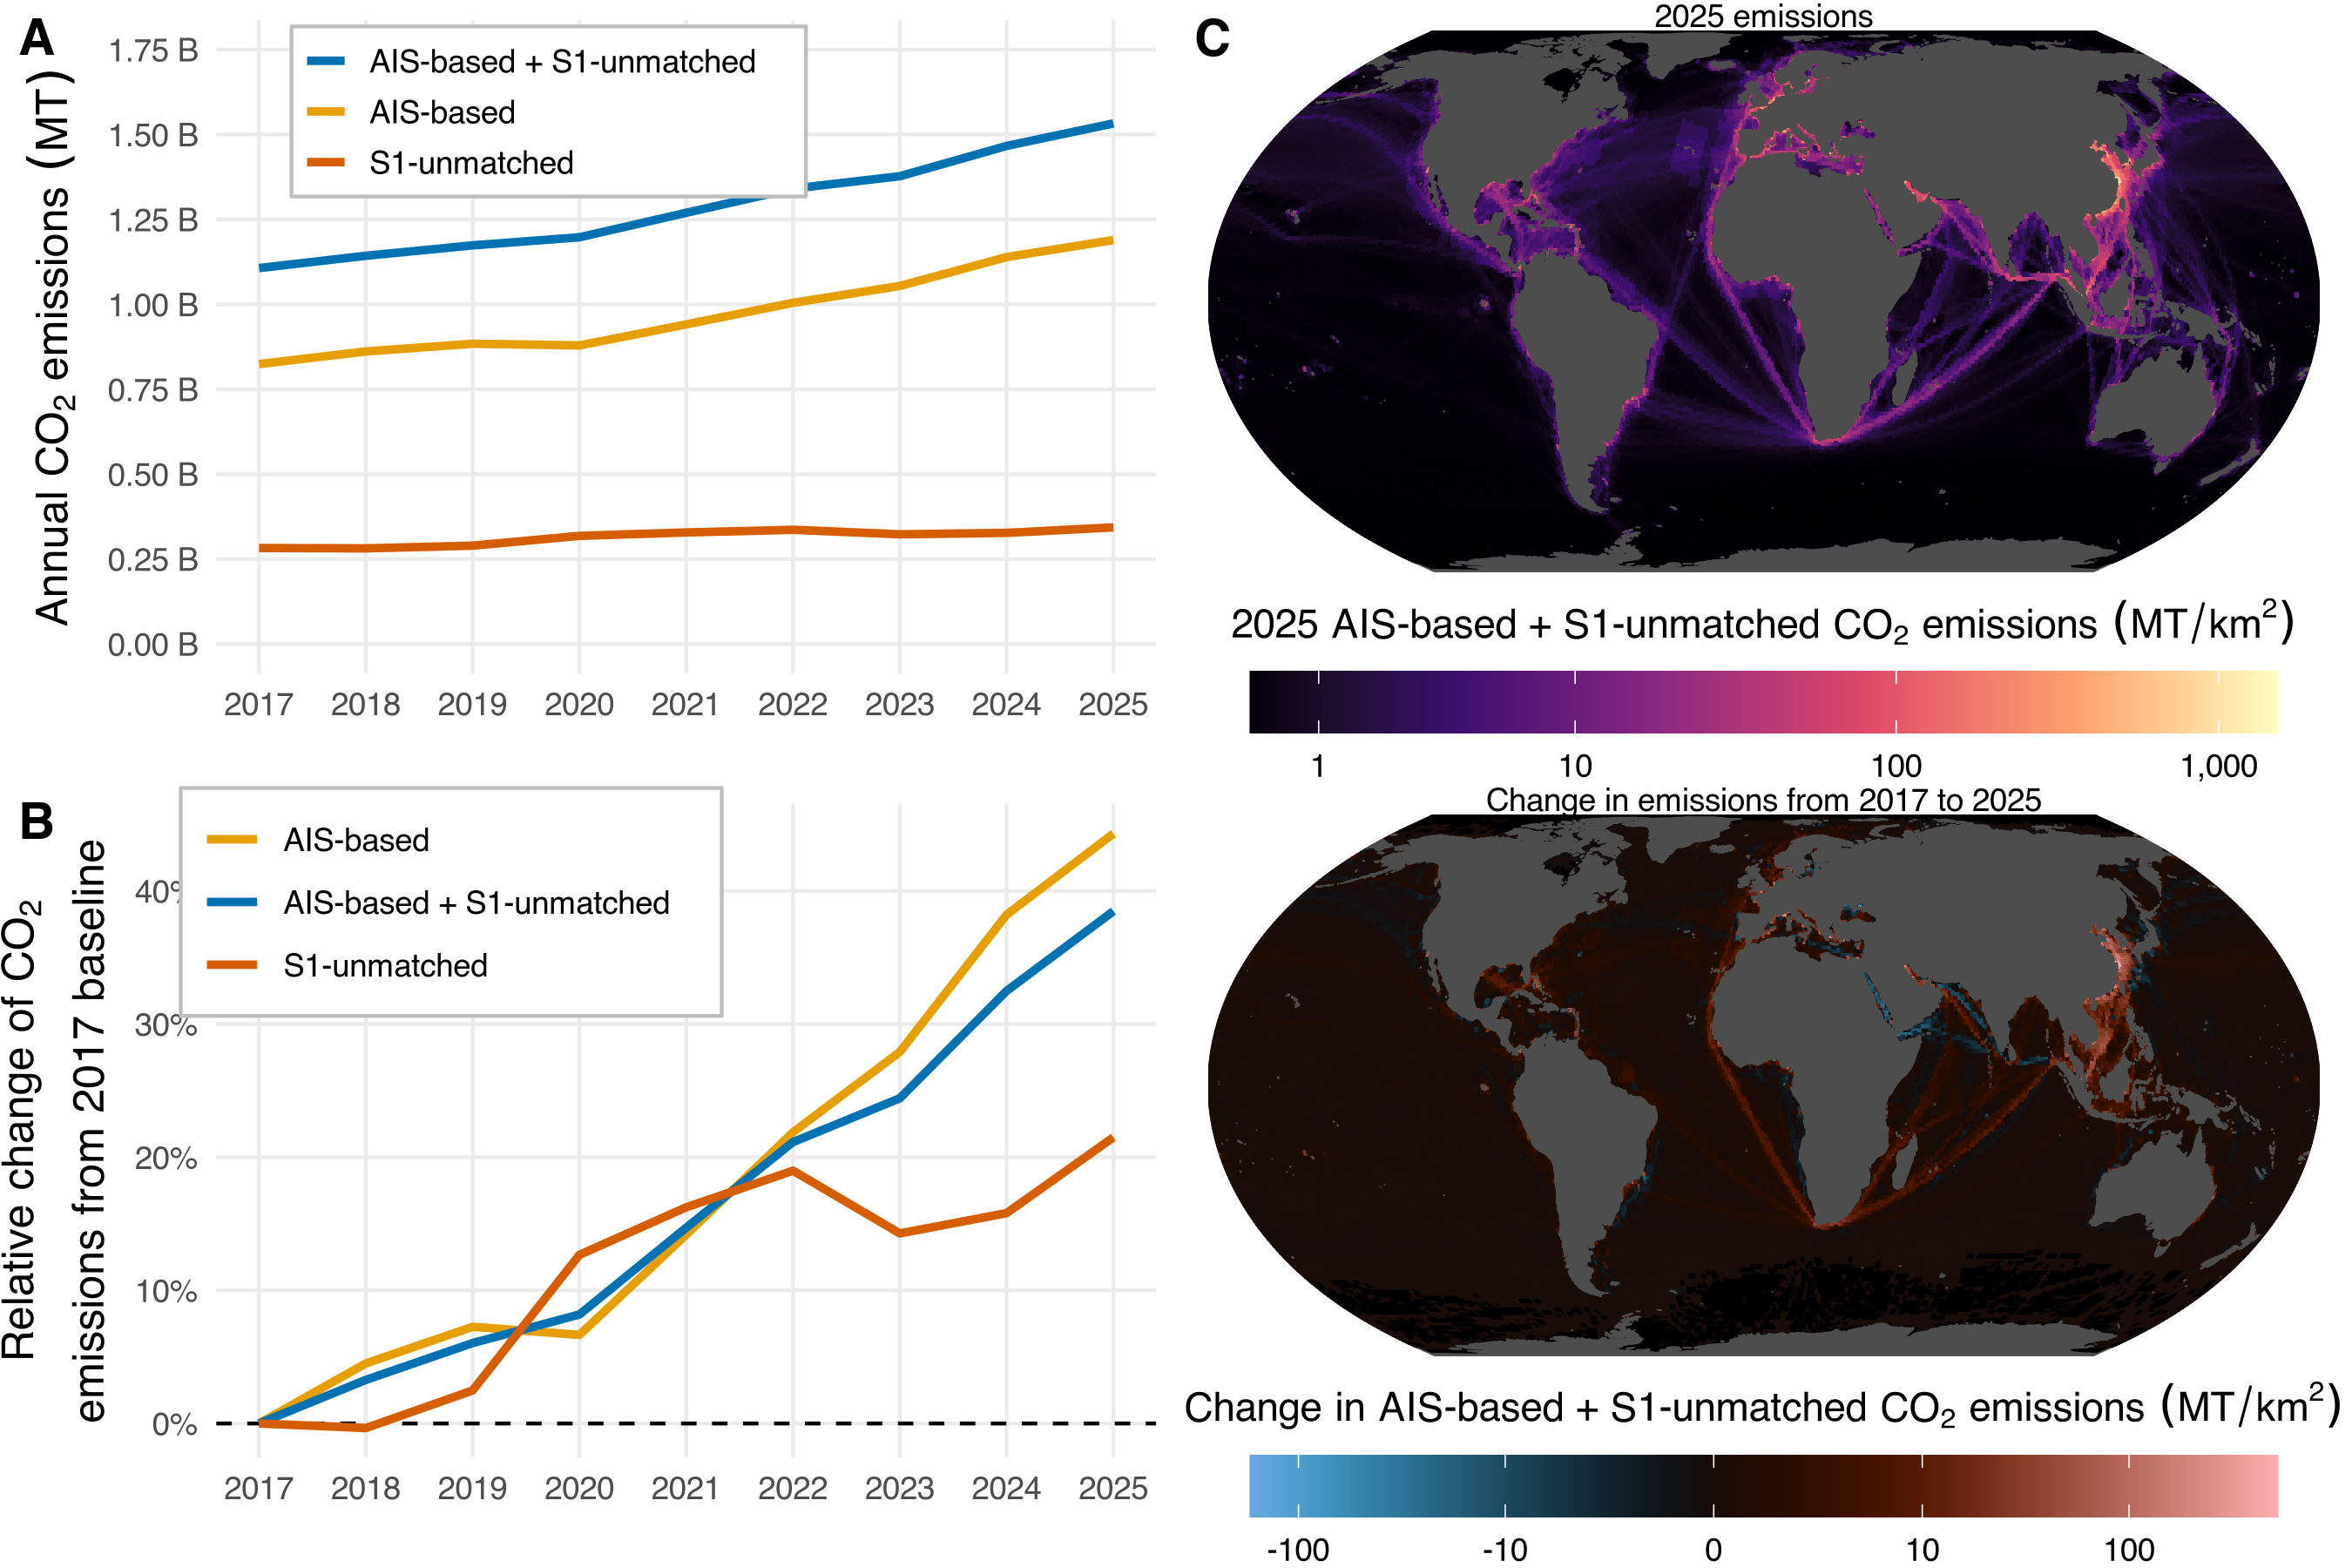
\includegraphics[width=\columnwidth]{figures/fig-emissions-by-data-source-and-maps-1.png}
    \caption{(a) Annual marine vessel CO$_{2}$ emissions, with each line colored based on the data source: `AIS-based' (emissions from AIS-broadcasting vessels whose AIS signal was received, estimated ping-by-ping from the observed activity of those vessels); `S1-unmatched' (emissions from vessels detected by S1 that could not be matched to an AIS-broadcasting vessel, either because the vessel is completely non-broadcasting or because its AIS signal was not received --- that is, vessels observed by radar but absent from the AIS record); and `AIS-based + S1-unmatched' (the aggregation of these `AIS-based' and `S1-unmatched' emissions, our fused total). (b) Relative change in annual marine vessel CO$_{2}$ emissions from a 2017 baseline, with each line colored based on the data source. (c) Spatial map of CO$_{2}$ emissions in 2025 (top) and change in CO$_{2}$ emissions between 2017 and 2025 (bottom), aggregated across AIS-based and S1-unmatched emissions, and shown at a 1x1 degree spatial resolution; emissions are area-normalized for each pixel (metric tonnes per square kilometer, shown on a pseudolog-10 scale).}
    \label{fig:fig-emissions-by-data-source-and-maps}
\end{figure}

Estimating S1-unmatched emissions offers new insights into the temporal trends and spatial patterns of global emissions (Fig. \ref{fig:fig-emissions-time-series-and-maps}). Although total emissions has generally been increasing (Fig. \ref{fig:fig-emissions-time-series-and-maps}a), the S1-unmatched share of emissions has generally been declining since 2021 (Fig. \ref{fig:fig-emissions-time-series-and-maps}b), consistent with a steady increase in AIS monitoring over the period. The time series data reveal strong seasonal trends and event-driven variations in marine GHG emissions. We see consistent dips during major holidays including Christmas, New Year’s Day, and Chinese New Year, as well as during the COVID-19 pandemic (Fig. \ref{fig:fig-emissions-time-series-and-maps}a and Supplementary Fig. \ref{fig:fig-pollutant-time-series}). Being able to spatially quantify S1-unmatched emissions fills important gaps in our current understanding of where marine vessel emissions take place, particularly in southeast Asia, China, the Caribbean, and the Mediterranean (Fig. \ref{fig:fig-emissions-time-series-and-maps}c), crucial for targeting policy or private sector interventions. Expressed as a share of each pixel's total emissions rather than as a magnitude, the pattern is sharper still (Fig. \ref{fig:fig-emissions-time-series-and-maps}c, bottom): the S1-unmatched contribution is concentrated over continental shelves and in coastal waters --- southeast Asia, west Africa, the Arctic, and southern South America --- while the major open-ocean shipping lanes, where large AIS-broadcasting vessels dominate, are close to zero. The brightest pixels are not, however, where the emissions are: pixels in which more than half of 2025 CO$_{2}$ is S1-unmatched make up 7.4\% of ocean pixels but only 4.7\% of emissions, while 77.1\% of emissions occur in pixels where the S1-unmatched share falls between 5\% and 50\%. Emissions monitoring based on AIS alone is therefore least complete precisely in the coastal waters where national jurisdiction, and the scope for intervention, is greatest. Our dataset also provides this sort of nuanced spatiotemporal information disaggregated by fishing and non-fishing vessels (Supplementary Fig. \ref{fig:fig-spatial-temporal-richness-by-fleet-total-pseudolog}). In 2025, 35\% of CO$_{2}$ emissions from fishing vessels were from S1-unmatched detections, and 20\% of CO$_{2}$ emissions from non-fishing vessels were from S1-unmatched detections.

\begin{figure}[H]
    \centering
    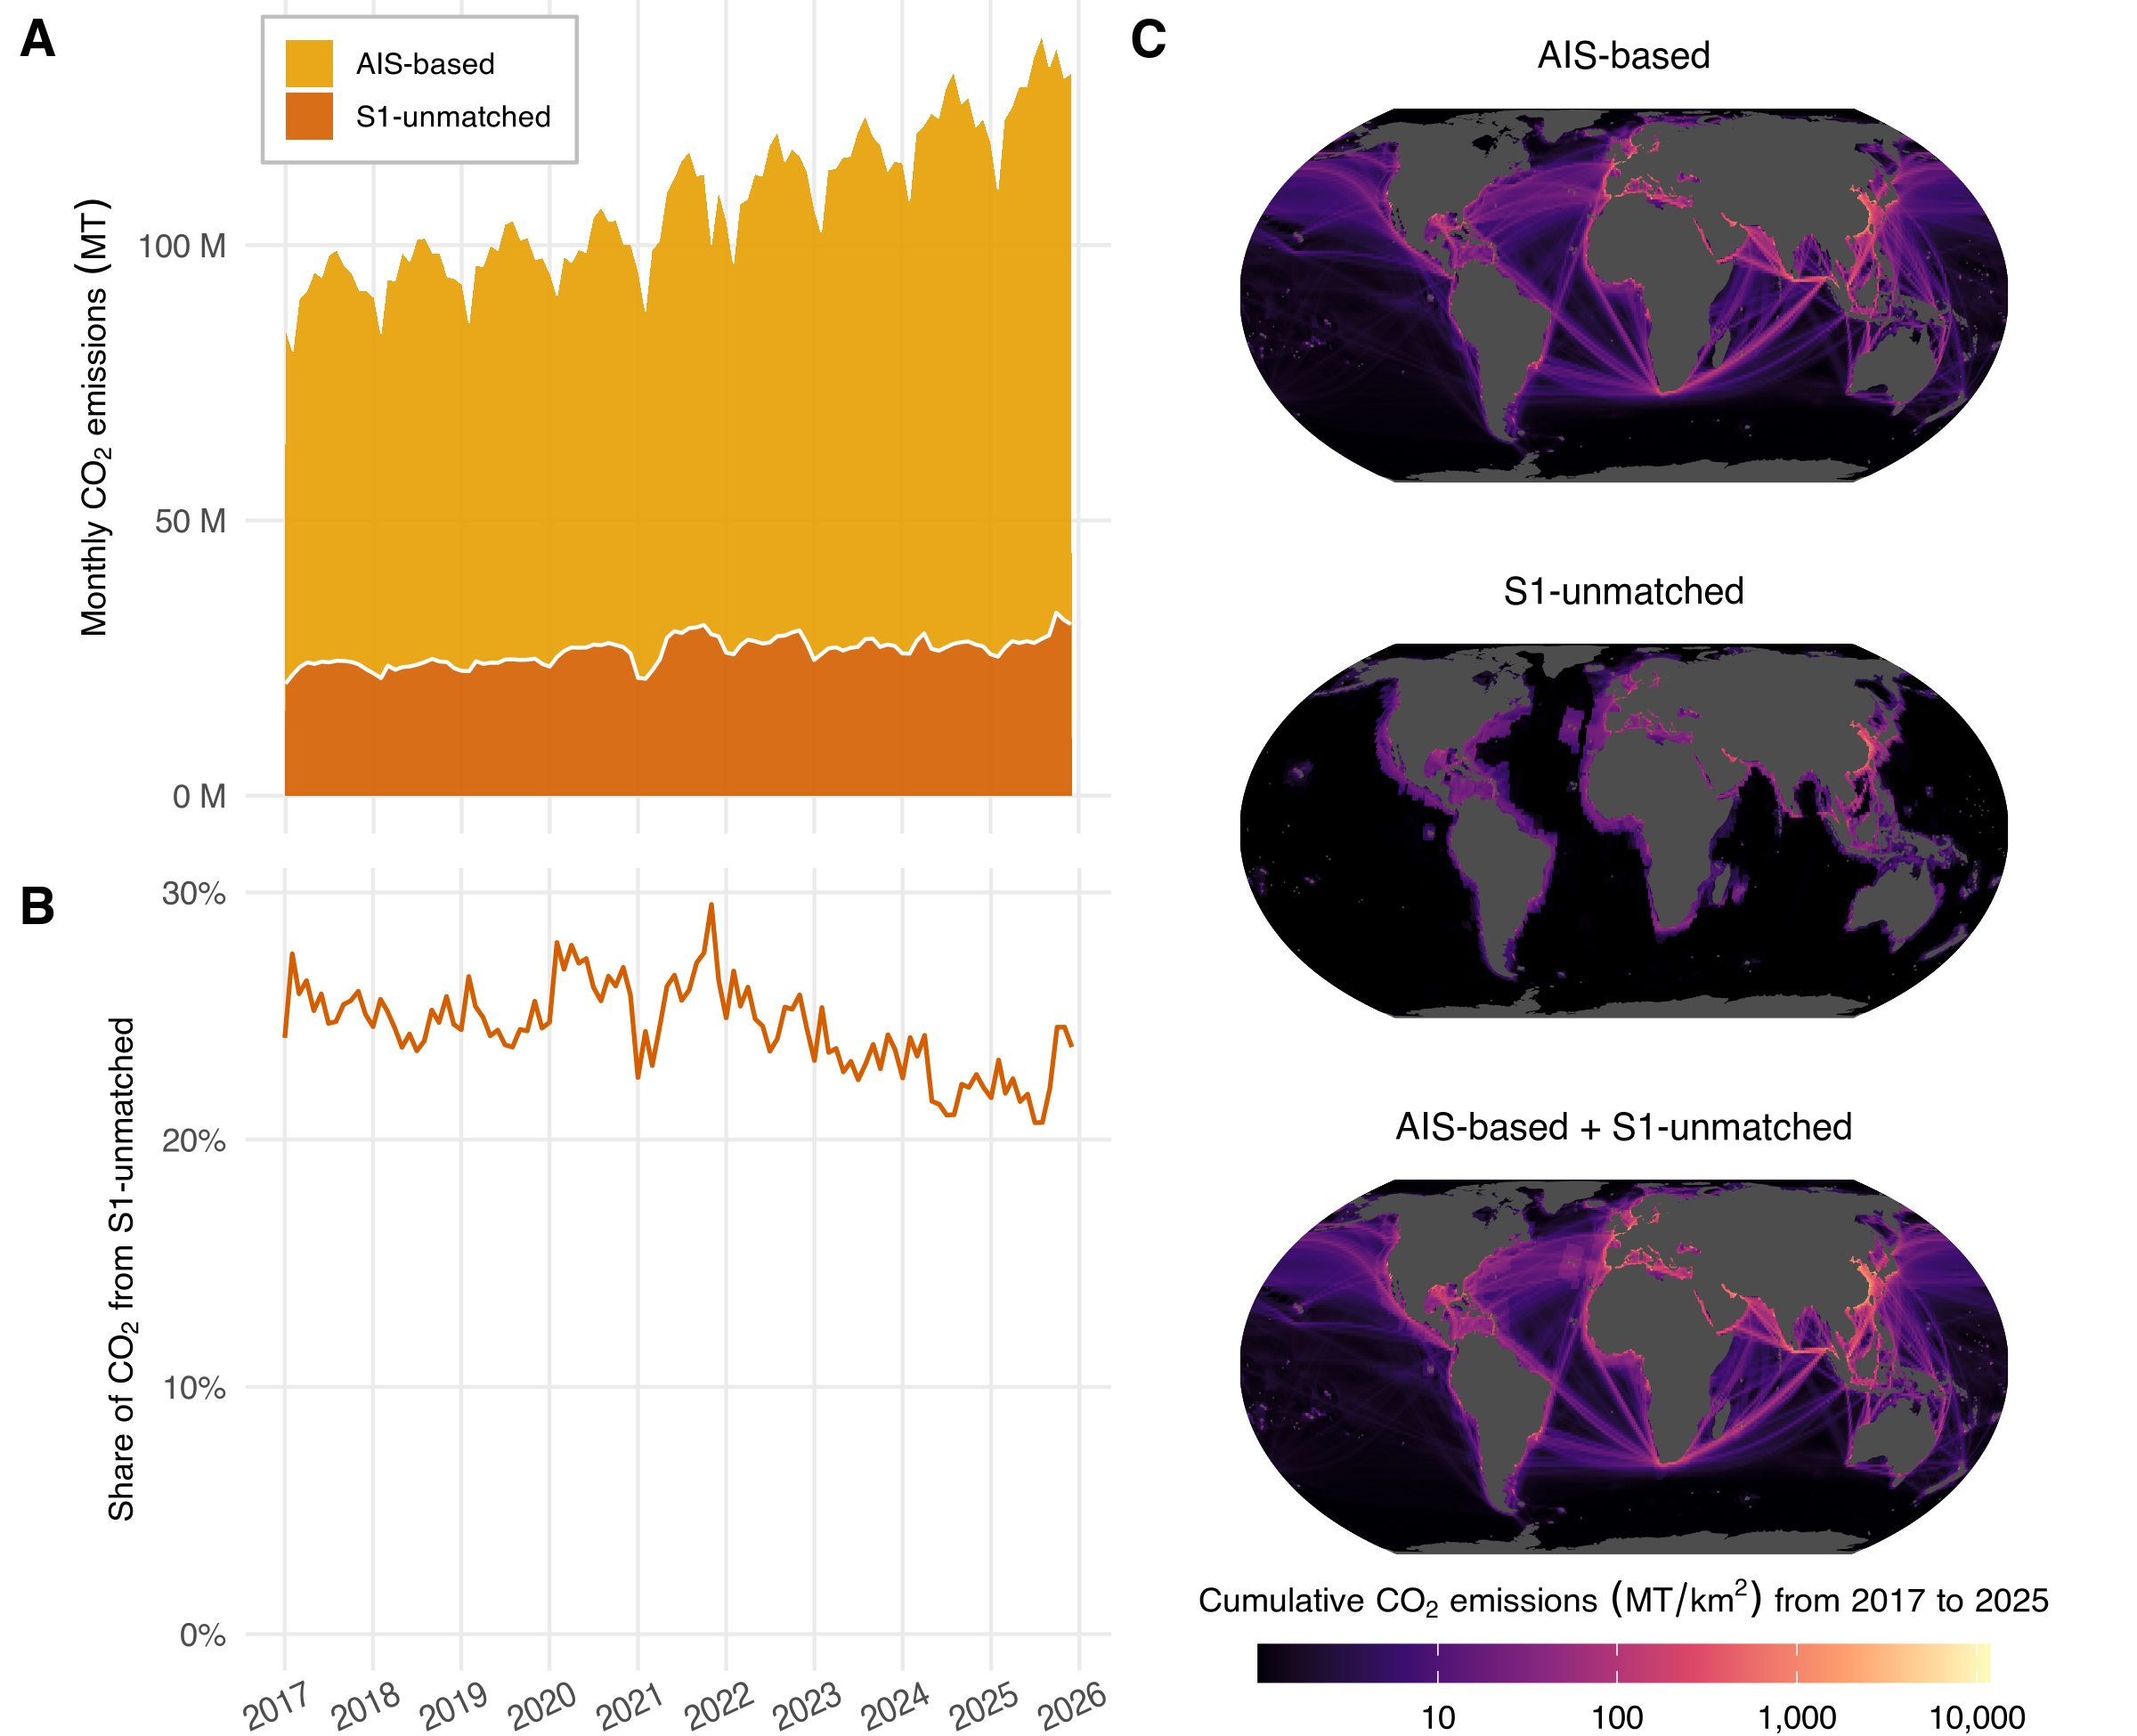
\includegraphics[width=\columnwidth]{figures/fig-emissions-time-series-and-maps-1.png}
    \caption{(a) Time series of monthly global CO$_2$ emissions, with each line colored based on the data source: `AIS-based' (emissions from AIS-broadcasting vessels whose AIS signal was received, estimated ping-by-ping from the observed activity of those vessels); `S1-unmatched' (emissions from vessels detected by S1 that could not be matched to an AIS-broadcasting vessel, either because the vessel is completely non-broadcasting or because its AIS signal was not received --- that is, vessels observed by radar but absent from the AIS record); and `AIS-based + S1-unmatched' (the aggregation of these `AIS-based' and `S1-unmatched' emissions, our fused total). (b) Time series of the monthly share of global CO$_{2}$ emissions attributable to S1-detected unmatched vessels. (c) Spatial distribution of 2025 CO$_{2}$ emissions from AIS-broadcasting vessels (top) and S1-detected unmatched vessels (middle), shown at a 1x1 degree spatial resolution; emissions are area-normalized for each pixel (metric tonnes per square kilometer, shown on a pseudolog-10 scale). The bottom map shows, for each pixel, the share of its 2025 CO$_{2}$ emissions that is S1-unmatched. Because this is a bounded percentage rather than a magnitude, it carries its own color scale, distinct from the one shared by the two maps above it. Every pixel carries a modeled value, so a pixel reading 0\% is one with no S1-unmatched emissions rather than one with no data. Note that panel b and the bottom map of panel c show the same quantity, in time and in space respectively, and that panel b's vertical axis does not start at zero.}
    \label{fig:fig-emissions-time-series-and-maps}
\end{figure}

Across the entire 2017 to 2025 time series, almost all S1-unmatched emissions (96.5\%) occurred inside the S1 footprint and in pixel-months that were imaged by S1 (Fig. \ref{fig:fig-spatial-coverage-footprint}). This makes sense because part of the Copernicus system's observation strategy for S1 is specifically focused on imaging coastal and shipping areas, where ship density is highest \cite{ESA2013S1Handbook}. Our machine learning model for predicting these emissions directly from observed S1 detection density achieves a high out-of-sample predictive performance (traditional R$^{2}$ = 0.94 and total percent error of -7.8\% for CO$_2$, Table \ref{tab:all_performance_metrics_table}). Only 3.4\% of S1-unmatched emissions occurred inside the S1 footprint but in pixel-months that weren't imaged by S1, requiring us to use a two-stage hurdle framework using both a classification model (F1 Score = 0.72) and a regression model (traditional R$^{2}$ = 0.69) to predict S1 detection density before predicting emissions (traditional R$^{2}$ = 0.94). Only 0.056\% of S1-unmatched emissions occurred outside the S1 footprint entirely, since most vessels operating in these open ocean areas use AIS.

Our vessel-level AIS-based emissions data provide a detailed understanding of marine vessel emissions across vessel classes and activity types (Fig. \ref{fig:fig-ais-data-richness}). We are able to distinguish activity between 37 classes of vessels, including 14 classes of fishing vessels; this makes our inventory the first to our knowledge that provides this level of emissions detail for fishing vessels. Container and bulk carriers, which transport much of the world's goods by sea, are the highest-emitting cargo classes (Fig. \ref{fig:fig-ais-data-richness}a-b). Oil tankers, which themselves transport fossil fuels, are the highest-emitting tanker type. These vessel classes are ranked similarly in other inventories \cite{johanssonGlobalAssessmentShipping2017, kramelGlobalShippingEmissions2021, yiHighresolutionGlobalShipping2025, mao2025greenhouse}, with the notable exception of the passenger category. Passenger vessels have a highly aggregated definition in our model, composed of several diverse vessel subclasses including ferries, cruise, Ro-Pax and yachts, which makes it the most numerous class in our fleet and consequently the largest emitting group in 2025 (Supplementary Fig. \ref{fig:figS-fleet-sankey-with-series-2025}). This and any further departure from other studies reflects our broader vessel coverage, which includes classes and sizes that are absent or underrepresented elsewhere—vessels below 25 m account for most passenger emissions in our inventory (Supplementary Fig. \ref{fig:figS-passenger-size-panels}, panel b), and fishing vessels are our second-largest class by vessel count (Supplementary Fig. \ref{fig:figS-fleet-sankey-with-series-2025}). Trawlers, which use an energy-intensive fishing technique in which nets are dragged through the water \cite{coello2015ais}, are the highest-emitting type of fishing vessel. Emissions from AIS-broadcasting vessels can also be assigned to port stays in particular countries and port-to-port voyages within- and between-countries by analyzing the movement tracks of each individual vessel (Fig. \ref{fig:fig-ais-data-richness}c and Supplementary Fig. \ref{fig:fig-emissions-by-country-and-activity-type}). Most emissions for cargo and tanker vessels occur during international trips, while most service and passenger vessel emissions occur within ports (Fig. \ref{fig:fig-ais-data-richness}c). China, Japan, and United States had the most CO$_{2}$ emissions during within-country domestic trips in 2025. China, Malaysia, and United States had the most CO$_{2}$ emissions during international trips that started or ended in these countries in 2025 (where the emissions from each trip are partitioned equally to its departure and arrival country). China, United States, and Indonesia had the most CO$_{2}$ emissions during port stays. Country totals for every activity type are summarized in Supplementary Fig. \ref{fig:fig-emissions-by-country-and-activity-type} and listed in Supplementary Table \ref{tab:top_countries_by_activity_type}. We note that roughly 5\% of AIS-enabled signals are actually attributable to AIS transponders that are not on vessels, but are rather on buoys, fish aggregating devices (FADs), navigation aids, offshore structures, fishing gear, and other objects. These non-vessel AIS signals are completely excluded from our analysis.


 \begin{figure}[H]
    \centering
    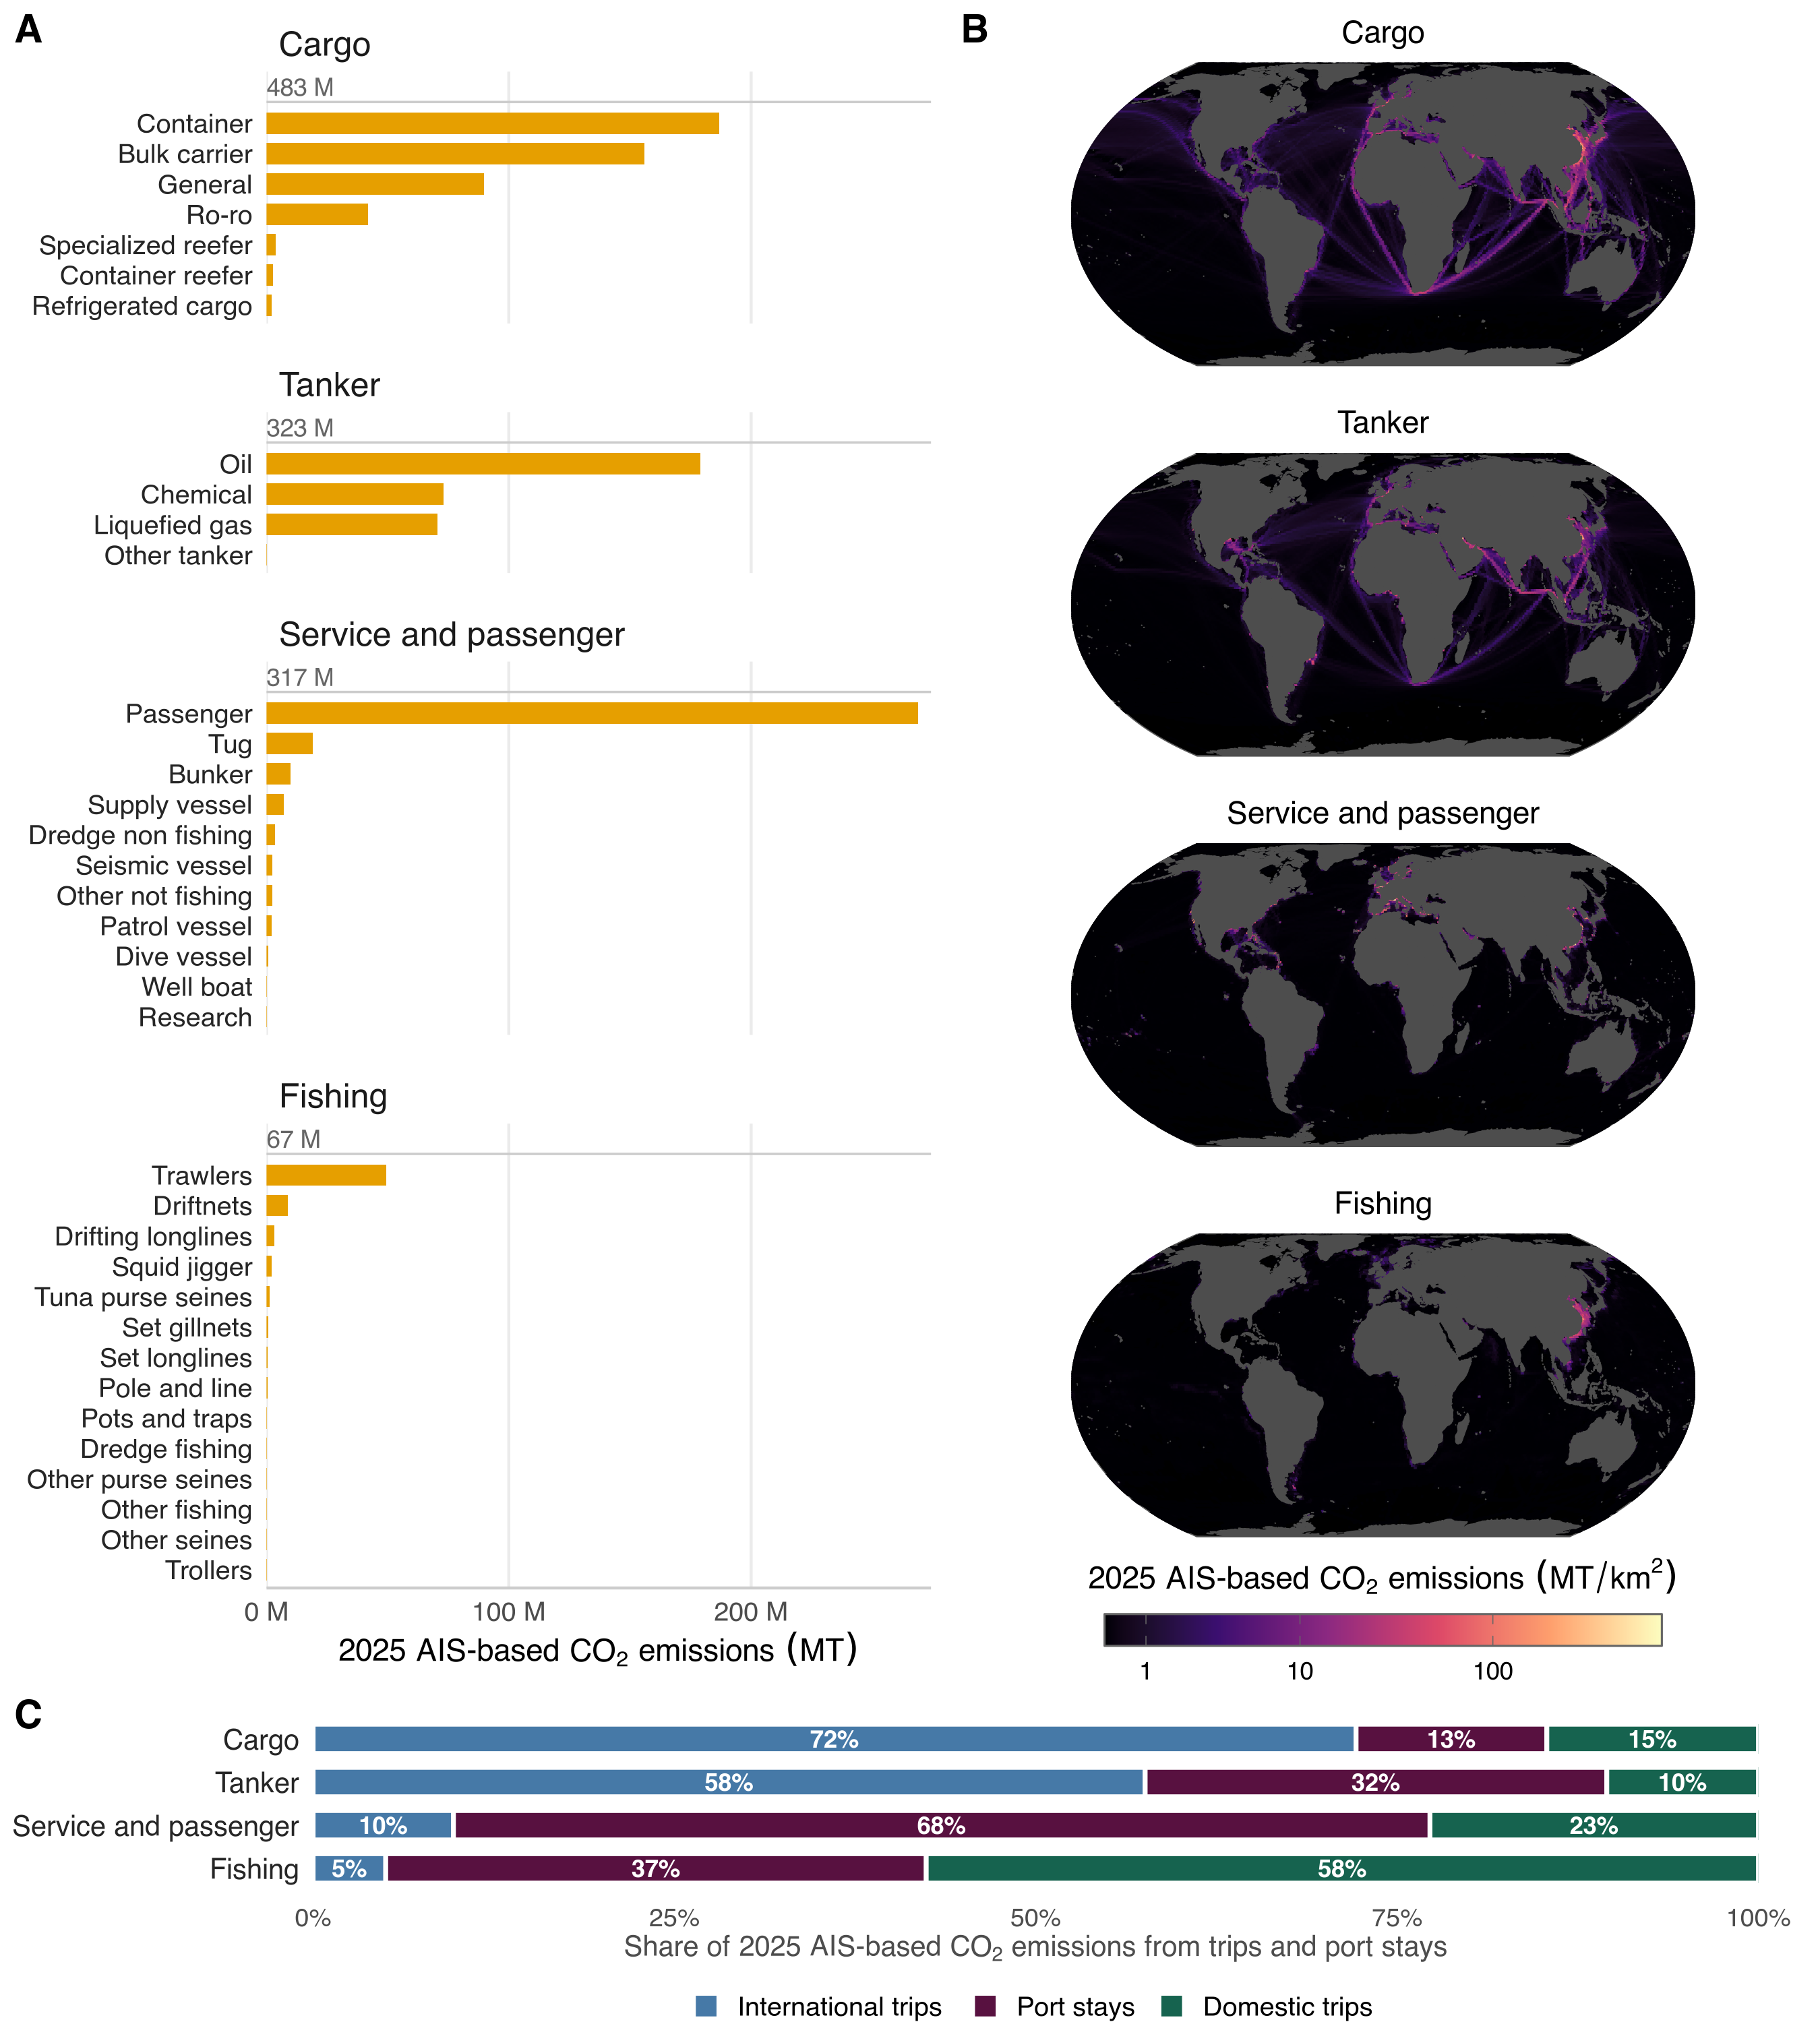
\includegraphics[width=\columnwidth]{figures/fig-ais-data-richness-1.png}
    \caption{Richness of AIS-broadcasting vessel emissions data, showing: (a) Total 2025 CO$_{2}$ emissions by vessel class for AIS-broadcasting vessels. Vessel classes are grouped into four families, with the total for each family shown above its bars; every class in a family is shown as its own bar, so panel heights differ with the number of classes. These totals are aggregated from the same gridded emissions shown in panel b, so the two panels describe exactly the same emissions and the bars sum to the mapped total. (b) Spatial distribution of 2025 CO$_{2}$ emissions from AIS-broadcasting vessels for each of those same vessel class families, shown at a 1x1 degree spatial resolution; emissions are area-normalized for each pixel (metric tonnes per square kilometer, shown on a pseudolog-10 scale). Families appear in the same order in both panels. (c) For each family, the share of CO$_{2}$ emissions attributable to international trips, port stays, and domestic trips (note that Panel c is not a decomposition of panel a: it covers only emissions that could be assigned to a trip or port visit that ended in 2025; each family sums to 100\% of its own assigned emissions).}
    \label{fig:fig-ais-data-richness}
\end{figure}

By developing new methods for inferring key missing vessel characteristics that are necessary for AIS-based emissions modeling, we can accurately estimate vessel-level emissions for a huge swath of the world's fleet that does not otherwise have the necessary vessel characteristic information in public registries. Of the roughly 775,000 AIS-broadcasting vessels in our analysis, we matched 139,000 (18\%) to public registries or proprietary databases, the majority of which (93,400) were IMO-registered. This allowed us to leverage vessel characteristics provided for these vessels from these databases. However, the vast majority of AIS-broadcasting vessels were not present in these registries, meaning that we needed to use model-derived vessel characteristics for between 83\% and 92\% of vessels, depending on the characteristic (Table \ref{tab:characteristic-availability}).  Because many large vessels are already listed with the IMO, the majority of our total CO$_{2}$ emissions come from these vessels (39\%); 19\% come from vessels listed on other registries; and 42\% come from vessels with no public registry information and which rely entirely on modeled vessel characteristics.

Using the vessel characteristic values that are derived from our machine learning models, we achieve an out-of-sample model performance of 0.85 traditional R$^{2}$ when comparing our daily vessel-specific CO$_{2}$ emissions estimates against those derived from a proprietary vessel registry dataset of over 15,000 vessel-specific fuel consumption values that were measured during at-sea trials (Fig. \ref{fig:fig-registered-data-performance}). If we were to instead estimate emissions with our model using only currently available public vessel characteristic data (i.e., the IMO provides lookup tables for average main engine power and design speed for different vessel types and sizes \cite{fourth2020greenhouse}), we would only achieve a predictive performance value of 0.73 traditional R$^{2}$. We also measured the performance of our model's ability to estimate annual vessel-level CO$_{2}$ emissions estimates by comparing our estimates to those available in the publicly available European Maritime Safety Agency’s Monitoring, Reporting, and Verification (MRV) database \cite{mrv_emissions}. Using a set of over 27,000 matched vessel-specific annual emissions estimates, we found a performance value of 0.84 traditional R$^{2}$ (Table \ref{tab:tab-performance-tolerance-table}).

The dataset also allows us to examine large-scale trends in marine vessel emissions for different parts of the ocean, and for different sectors of the global economy. Although vessel activity in the Southern Ocean represents a very small fractions of the world's marine vessel emissions (0.04\%), it represents the part of the world experiencing the highest growth rate of marine vessel emissions (267\%) (Supplementary Fig. \ref{fig:fig-emissions-marine-ocean-other}, Supplementary Table \ref{tab:emissions_by_ocean_summary_tbl}). These polar estimates are primarily driven by AIS-broadcasting vessels, with only a small fraction S1-unmatched (0.88\% in the Southern Ocean; Supplementary Table \ref{tab:emissions_by_ocean_summary_tbl}, Supplementary Fig. \ref{fig:fig-annual-emissions-by-ocean-and-data-source}). Polar regions have extremely limited S1 coverage (only 0.06\%  of pixel-months in the Southern Ocean were imaged by S1), meaning that trends there may be more susceptible to AIS adoption biases. This reflects the growing importance of monitoring marine vessel activity in the world's extreme latitudes. 

Our AIS-based series agrees with other bottom-up inventories early in the study period but exceeds them in later years (Fig. \ref{fig:fig-emissions-inventory-comparison}, panel a). The fused total (AIS-based + S1-unmatched) sits above every other inventory across the whole time period, and we see a similar gap in magnitude when comparing against the top-down EDGAR and CEDS inventories (Fig. \ref{fig:fig-emissions-inventory-comparison}, panel b). Looked at more broadly, our total fused marine vessel emissions accounted for roughly 3.4-3.5\% of all emissions globally in 2022 (according to CEDS and EDGAR global inventories, respectfully \cite{hoeslyHistorical17502014Anthropogenic2018,JRC143227}), and 15.5-15.7\% of all transportation-related CO$_{2}$ emissions (a share consistent with the 14.2\% of EU transportation emissions attributed to the maritime sector by the European Maritime Safety Agency in 2022 \cite{emsa2025}).  In terms of trends, our fused total emissions estimate grew at a compound annual growth rate of 3.86\%, more than twice the rate of any other AIS-based marine vessel emissions inventory, about four times the rate of global emissions across all sectors (0.91\%/yr in CEDS, 0.98\%/yr in EDGAR), and about seven to eight times the rate of  other transportation sectors (0.54\%/yr in CEDS, 0.47\%/yr in EDGAR) (Supplementary Fig. \ref{fig:figS-inventory-comparison-all-sources}, Supplementary Table \ref{tab:inventory_growth_comparison}). 


\begin{figure}[H]
    \centering
    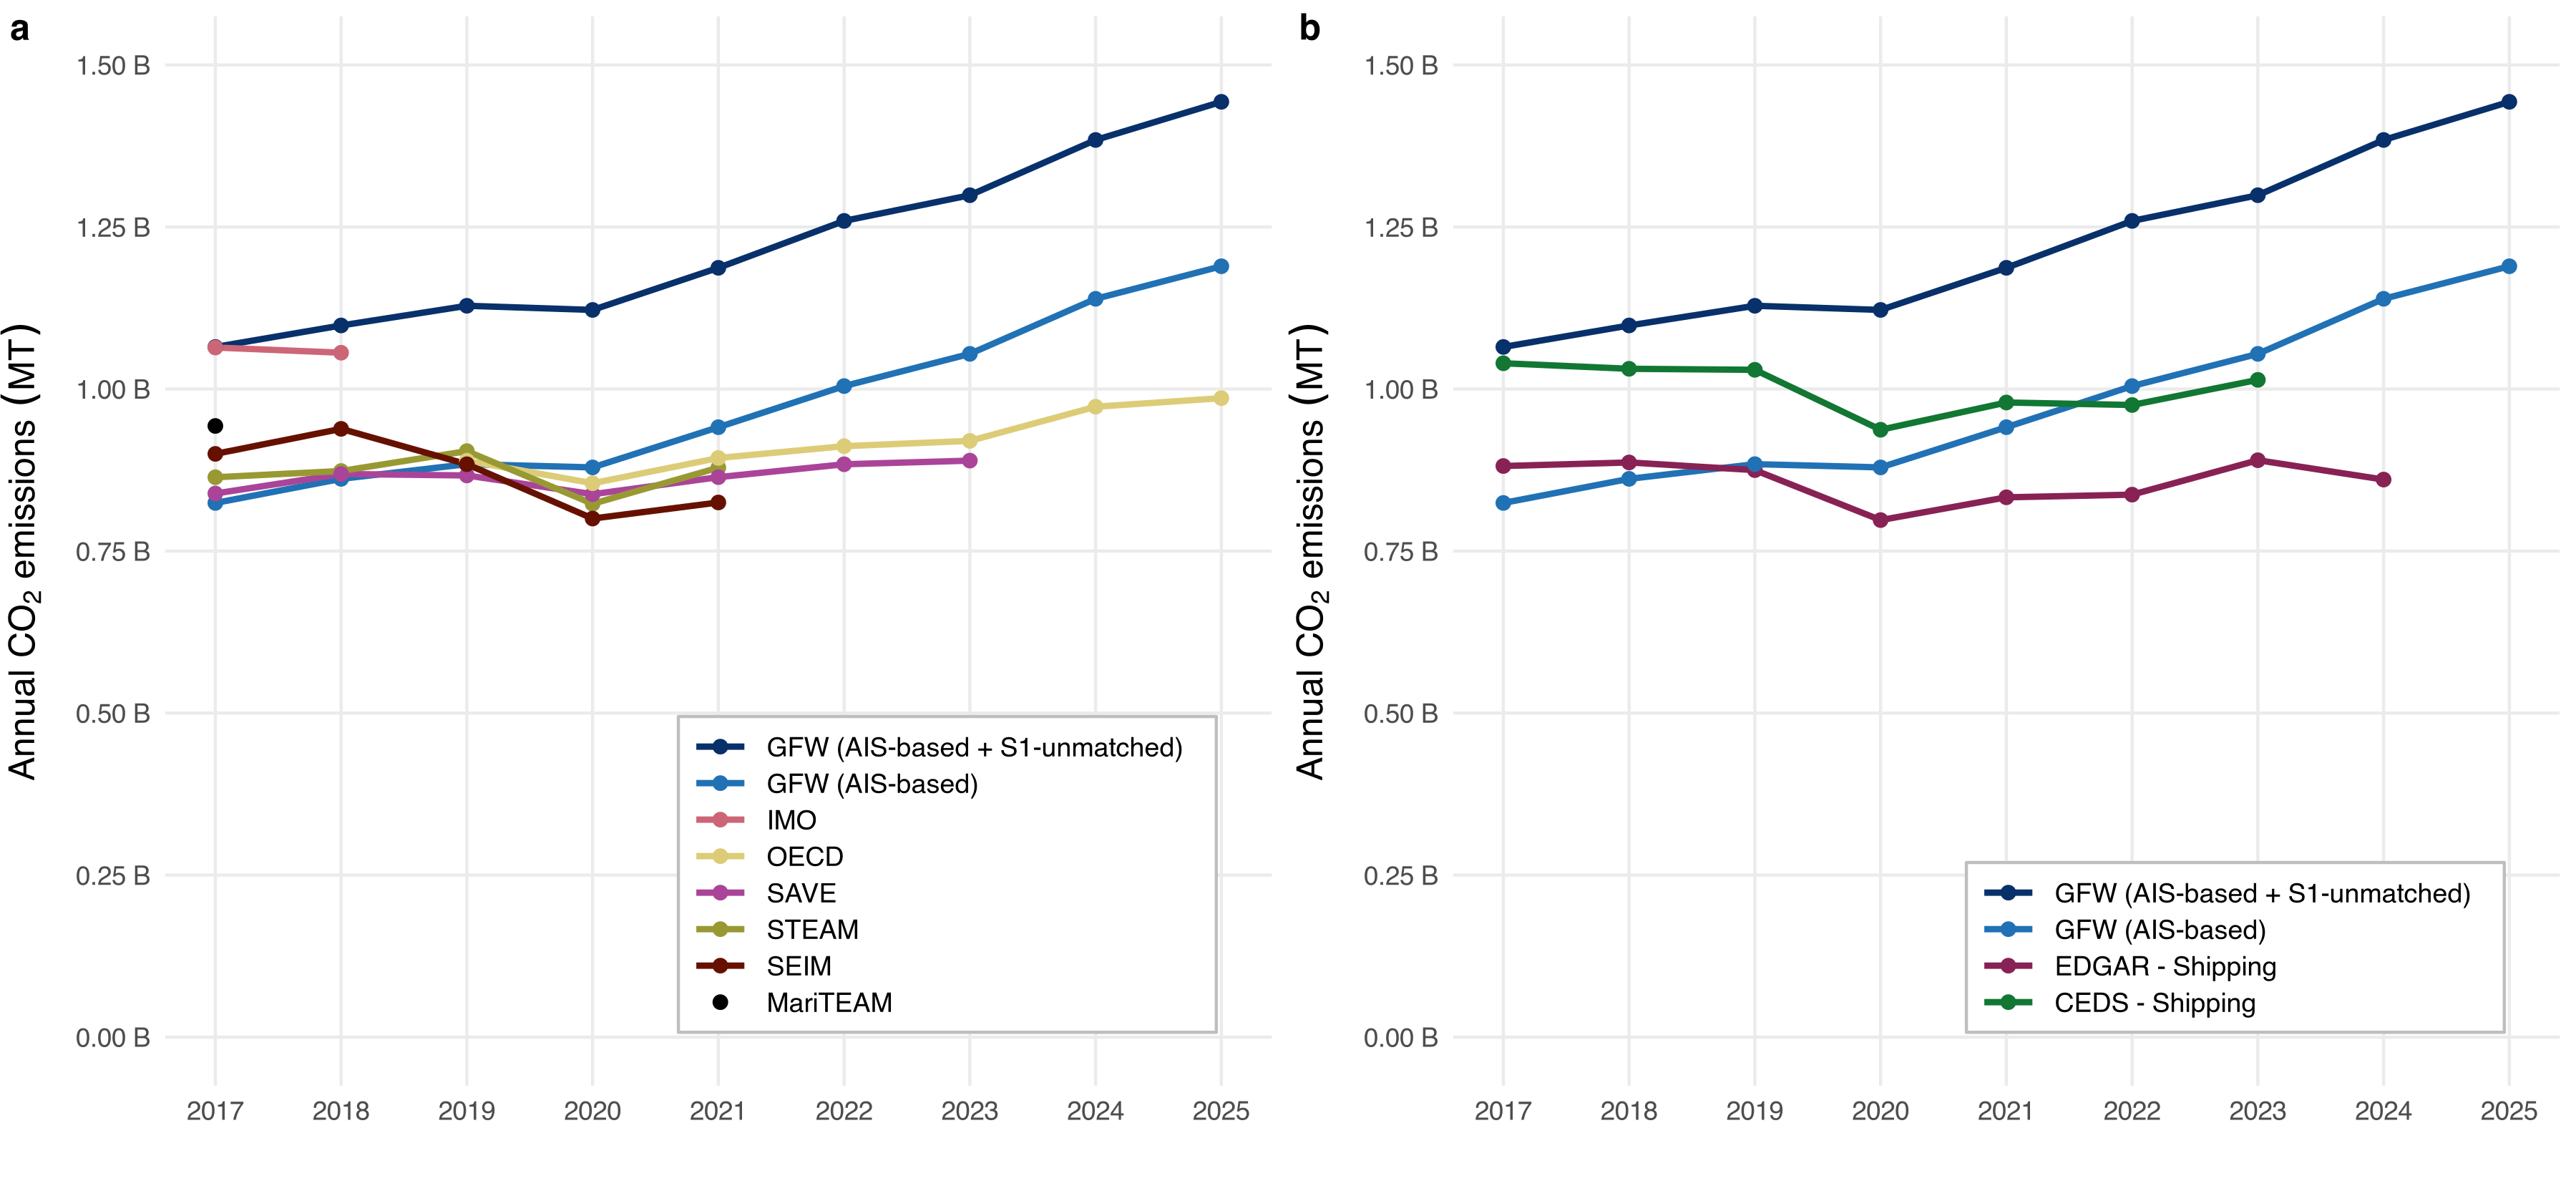
\includegraphics[width=\columnwidth]{figures/fig-emissions-inventory-comparison-1.png}
    \caption{ (a) Annual CO$_{2}$ emissions from our AIS-based and fused (AIS-based + S1-unmatched) estimates against the other major bottom-up, AIS-based marine vessel emissions inventories (STEAM, SEIM, MariTEAM, OECD, SAVE, and the Fourth IMO GHG Study). (b) The same two series against the top-down EDGAR and CEDS shipping emissions inventories, which are derived from fuel statistics rather than from individual vessel activity.}
    \label{fig:fig-emissions-inventory-comparison}
\end{figure}

\section{Discussion}

High-resolution emissions data for marine vessels are essential for designing, implementing, and evaluating policies aimed at reducing them. However, incomplete vessel tracking data and technical data processing challenges have previously hindered progress \cite{chen2024analysis}. Our new data and methodology overcome these challenges by providing the spatiotemporal data necessary for analyzing interventions that could mitigate the GHG emissions that drive climate change, as well as other air pollutants that impact ambient air quality and health. Our data could also be used to quantify the spatial health impacts of air pollution related to shipping and fishing activity \cite{zhang2021global}, along with the associated environmental justice implications.

There are three main implications of the results: First, the spatial and temporal detail of our dataset makes it directly relevant for climate change and air quality policy. Carbon pricing, fuel standards, emissions control areas, port queuing reforms, and vessel speed reduction programs all require credible baselines and measurable outcomes. Our estimates provide such a baseline for both broadcasting and non-broadcasting activity, including vessels that would be missed by AIS-only inventories. This is especially relevant for the IMO's effort to move international shipping toward net-zero greenhouse gas emissions by 2050 by implementing a carbon market for international shipping emissions by vessels over 5,000 gross tonnage \cite{imo_carbon_price, IMO2025NetZero, kang2026maritime}. Further, the European Union Emissions Trading System has been expanded to include marine transportation under the EU emissions cap, and to subject vessel activity to and from European Economic Area ports to a carbon price \cite{kotzampasakis2025maritime}. Implementing a carbon market based on limiting emissions intensity (the amount of emissions per unit of activity or production) could also be an effective strategy for mitigating marine vessel emissions, even with a growing number of vessels. Carbon markets based on emissions-intensity standards rather than absolute emissions caps, such as India's emerging carbon market \cite{gupta2023assessing}, allow economic growth while continuing to incentivize improvements in emissions efficiency. This policy design is consistent with a review paper on current marine vessel emissions datasets, which concluded that measures aimed at increasing technical efficiency of ships could be an effective way to decouple emissions growth from global trade demand \cite{dengreview}.

Second, our data can be used to calculate the climate externality social cost (SC) associated with marine vessel activity, which can be compared against the economic value of the activities; we conduct a simple version of that calculation here. We first focus on non-fishing vessels (e.g., cargo ships and tankers) and compare their climate externalities with the value of goods transported by sea. Multiplying our estimated emissions of carbon dioxide, methane, and nitrous oxide from non-fishing vessels by the corresponding social costs of carbon (283 USD/MT \cite{moore2024synthesis}), methane (2,900 USD/MT \cite{wang2023damage}), and nitrous oxide (49,600 USD/MT \cite{wang2023damage}) yields an estimated annual global climate externality of 338 billion USD in 2021 (Supplementary Table \ref{tab:social_cost_summary_tbl}). This amounts to about 5\% of the total value of goods transported by maritime trade, based on an estimated 6.63 trillion USD in global seaborne trade in 2021 \cite{hoffmeister2022developing}. Repeating this calculation for fishing vessels yields an estimated annual global climate externality of 23 billion USD in 2022 (Supplementary Table \ref{tab:social_cost_summary_tbl}). This amounts to about 15\% of the global first-sale value of capture fisheries, which totaled 159 billion USD in 2022 \cite{fisheries2024state}. Our voyage-level emissions dataset can be used to estimate the climate externalities associated with country-to-country trade flows, enabling the construction of metrics such as the social cost per dollar of traded goods or the social cost per metric tonne of cargo transported. For vessels tracked with AIS, these externality costs can also be assigned to individual port-to-port voyages. Beyond their contribution to climate change, marine vessels emit air pollutants that impose substantial human health costs that have yet to be fully understood. \cite{zhang2021global}.

Third, our methodology and data can help address a broader challenge in environmental monitoring: temporal trends in environmental variables are often confounded by changes in monitoring effort. For marine vessel emissions, this challenge arises because the adoption of AIS and the number of vessels being tracked have increased over time, causing existing methods to overestimate the growth of at-sea emissions by 15.9\%. Similar biases may arise for other environmental variables when monitoring expands over time, such as the discovery of invasive species \cite{costello2003pattern}. By combining two independent data sources, our approach is more robust to changes in monitoring effort than methods that rely on a single source and therefore produces more accurate estimates of environmental change. The same framework could be applied in other settings where changes in monitoring complicate the measurement of long-run environmental trends.

Our approach is complementary to, rather than a replacement for, efforts to improve AIS data quality. Any AIS-derived inventory faces two distinct gaps: vessels that never broadcast, and broadcasting vessels whose signals are not received. Trajectory reconstruction addresses the second but cannot address the first. Reconstruction also cannot resolve the confound between monitoring and activity: because reconstruction methods are calibrated on observed AIS, discrete shifts in coverage — such as the 2022 adoption of D-AIS or the 2021 loss of terrestrial reception in Chinese waters (Supplementary Note \ref{sec:ais-receiver-types}) — propagate into reconstructed trajectories. S1 observation effort is independent of AIS coverage, which is what allows our estimates of the emissions trend to be robust to it. The value of our framework is therefore that it tolerates incomplete AIS: unmatched detections absorb emissions from both never-broadcasting vessels and broadcasting vessels with unreceived signals, so comprehensive emissions can be recovered without first achieving a "perfect" AIS reconstruction.

Several methodological limitations remain. One key assumption is that S1-unmatched emissions can be inferred from the relationship between S1 detections and AIS-based emissions for matched vessels. We believe this is a reasonable assumption for several reasons.  First, many unmatched S1 detections likely correspond to AIS-broadcasting vessels that are not observed in the AIS data because of transmission gaps or poor reception quality. In these cases, the relationship between S1 vessel detections and emissions would hold perfectly since these unmatched vessels are in fact just AIS-broadcasting vessels that happen to not be observed by AIS at a given point in time. Second, our model accounts for vessel length, a proxy for main engine power that is one of the primary determinants of emissions in AIS-based models and is applicable to virtually all vessels powered by internal combustion engines. Third, since fishing and non-fishing vessels are known to have different emissions factors \cite{coello2015ais}, we account for this by differentiating detections between fishing and non-fishing vessels. Finally, our model incorporates spatiotemporal features that allow the relationship between detections and emissions to vary across space and time. Consequently, if AIS-broadcasting and S1-unmatched vessels operating in a given place and time have similar characteristics, the relationship between detections and emissions is expected to be similar as well. 

Another limitation is that the relationship between detections and emissions may fail to hold for non-broadcasting vessels if their emissions factors differ substantially from the IMO values we use to convert energy use into emissions \cite{fourth2020greenhouse}. This could arise, for example, if non-broadcasting vessels disproportionately use newer and more efficient engine or fuel technologies that were not widely represented when the IMO emissions factors were developed in 2020; this would have the impact of biasing our S1-unmatched emissions estimates too high. Conversely, if non-broadcasting vessels instead use severely outdated and inefficient engine technologies, this this would have the impact of biasing our S1-unmatched emissions estimates too low. This highlights one of the primary limitations of the AIS model our methodology builds upon. Since information on the fuel type used by individual vessels is generally not publicly available, we rely on weighted average emissions factors from the IMO \cite{fourth2020greenhouse}. Vessel-level emissions estimates based on average emission factors may be biased if a particular vessel's engine or fuel type is not well represented in the global fleet. This could be an important consideration when using the model to explore policies aimed at technological engine changes and fuel switching. However, when this type of vessel-level information becomes publicly available, our modeling framework could easily be adapted to incorporate it. Despite the fact that we do not currently explicitly account for vessel-level fuel type, our vessel-level emissions model still achieves high performance when validated against two fully independent vessel-level datasets (Figs. \ref{fig:fig-registered-data-performance} - \ref{fig:fig-mrv-performance}). 

The difference between our AIS-based emissions and other bottom-up inventories is primarily one of fleet scope rather than of the emissions modeling itself (Supplementary Note \ref{sec:methods-comparison}). Global AIS-based emissions are likely understated whenever heavy reliance on registry-defined fleets leaves low-information vessels out of scope. The vessels in our analysis are not limited to only those that are registered, but rather includes all vessels that carry AIS; the fleet thus expands with increasing uptake of AIS among vessels, with our estimated emissions growth mostly carried by low-information vessels. This indicates that the other bottom-up inventories, and our own early years, likely miss part of the global fleet (Supplementary Note \ref{sec:inventory-comparison}). Our data fusion approach extends on this even further, expanding our estimates to include large vessels that appear in neither registries nor AIS, which also explains the magnitude gap with the top-down EDGAR and CEDS inventories. 

Our estimated growth rate indicates that marine vessel emissions are growing significantly faster than other inventories indicate, which requires more careful inspection. For our AIS-based results, this is largely driven by smaller vessels and certain vessel classes (e.g., passenger and fishing vessels) that: a) our inventory uniquely captures compared to other inventories; and b) also happen to be growing the fastest, both in terms of number of vessels and amount of emissions (Supplementary Figs. \ref{fig:figS-fleet-growth-by-year} - \ref{fig:figS-fleet-sankey-with-series-2025}). That only tells part of the story though -- these AIS-based emissions are increasing due to a combination of true increased activity, increasing AIS reception quality over time due to dynamic-AIS, as well as increased use of AIS among these vessels. Our data fusion approach allows us to at least partially disentangle these conflating effects. Looking at our S1 detection data, we see that the fraction of vessel detections matched to AIS is generally increasing over time, particularly for small vessels (Supplementary Fig. \ref{fig:figS-ais-carriage-saturation-by-size}). This tells us that indeed some of the increasing trend in AIS emissions is due to increased use of AIS. So within our data fusion framework, the emissions from these vessels is simply transferred from our S1-unmatched component to our AIS-based component as soon as they begin carrying AIS. However, even increasing adoption of AIS does not fully explain the scale of increasing emissions: although unmatched detections of small vessels are going down slightly over time --consistent with vessels adopting AIS -- matched detections are going up much more significantly -- indicating that there is simply more vessel activity. This provides new evidence supporting the concept of the `blue acceleration' and the expansion of human activity in the oceans \cite{jouffray2020blue}. However, we acknowledge that even when using data fusion, our approach is limited by the observational capacity of both AIS and S1. Neither AIS nor S1 have good coverage for very small vessels (i.e., $<$15m), and S1 is completely unable to capture wood and fiberglass vessels. This means that the magnitude of our fused approach is likely an underestimate of true global marine vessel emissions writ large. There also may be many small and coastal vessels that could not be detected by S1 in early years of our dataset due to detection limitations with S1, but which eventually adopt AIS. This could bias our increasing trend upwards compared to the true trend in activity, even when looking at our fused estimates. Further research could help further disentangle the magnitude and trends of small and coastal vessels. An exciting area of future work would be to incorporate new satellite sensors into our data fusion framework to better capture activity from small vessels (e.g., optical imagery from Sentinel-2 or PlanetScope \cite{wei2026satellite}).

% Still, even confined to non-fishing vessels of 150m and above---the segment of the fleet where AIS use was already widespread at the start of our series , and thus where measured growth reflects activity at sea and AIS quality rather than expanding AIS use---our AIS-based emissions grew at a compound annual rate of 3.20\%, nearly twice that of the fastest-growing bottom-up inventories, more than three times that of global emissions across all sectors, and about six to seven times that of all other transportation modes combined (Supplementary Fig. \ref{fig:figS-inventory-comparison-all-sources}, Supplementary Table \ref{tab:inventory_growth_comparison}).

Accurately measuring emissions is a necessary step towards reducing them. To date, quantifying emissions from vessels in the ocean has suffered from incomplete monitoring at-sea and the opaque nature of vessel characteristics. We fuse two satellite-based data sources and by doing so, are are able to track emissions from both broadcasting and non-broadcasting activity. Furthermore, by estimating key emissions modeling vessel characteristics for hundreds of thousands of vessels, we now have a comprehensive and high resolution picture of emissions from large marine vessels. This can serve as the foundation for interventions aimed at decarbonizing the marine sector and reducing the health impacts of marine air pollution.

\section*{Methods}

Our use of a large language model as a programming and editing assistant in preparing this work, and the limits placed on it, are documented under `Use of generative AI' below.

This work relies on multiple sources of spatial and tabular data to assess marine vessel emissions globally. We use AIS data, vessel registry information and Sentinel-1 (S1) derived data to construct our AIS-based emission model and the S1-unmatched emissions model (Fig. \ref{fig:gfw_emissions_framework_flowchart}).

\begin{figure}[H]
    \centering
    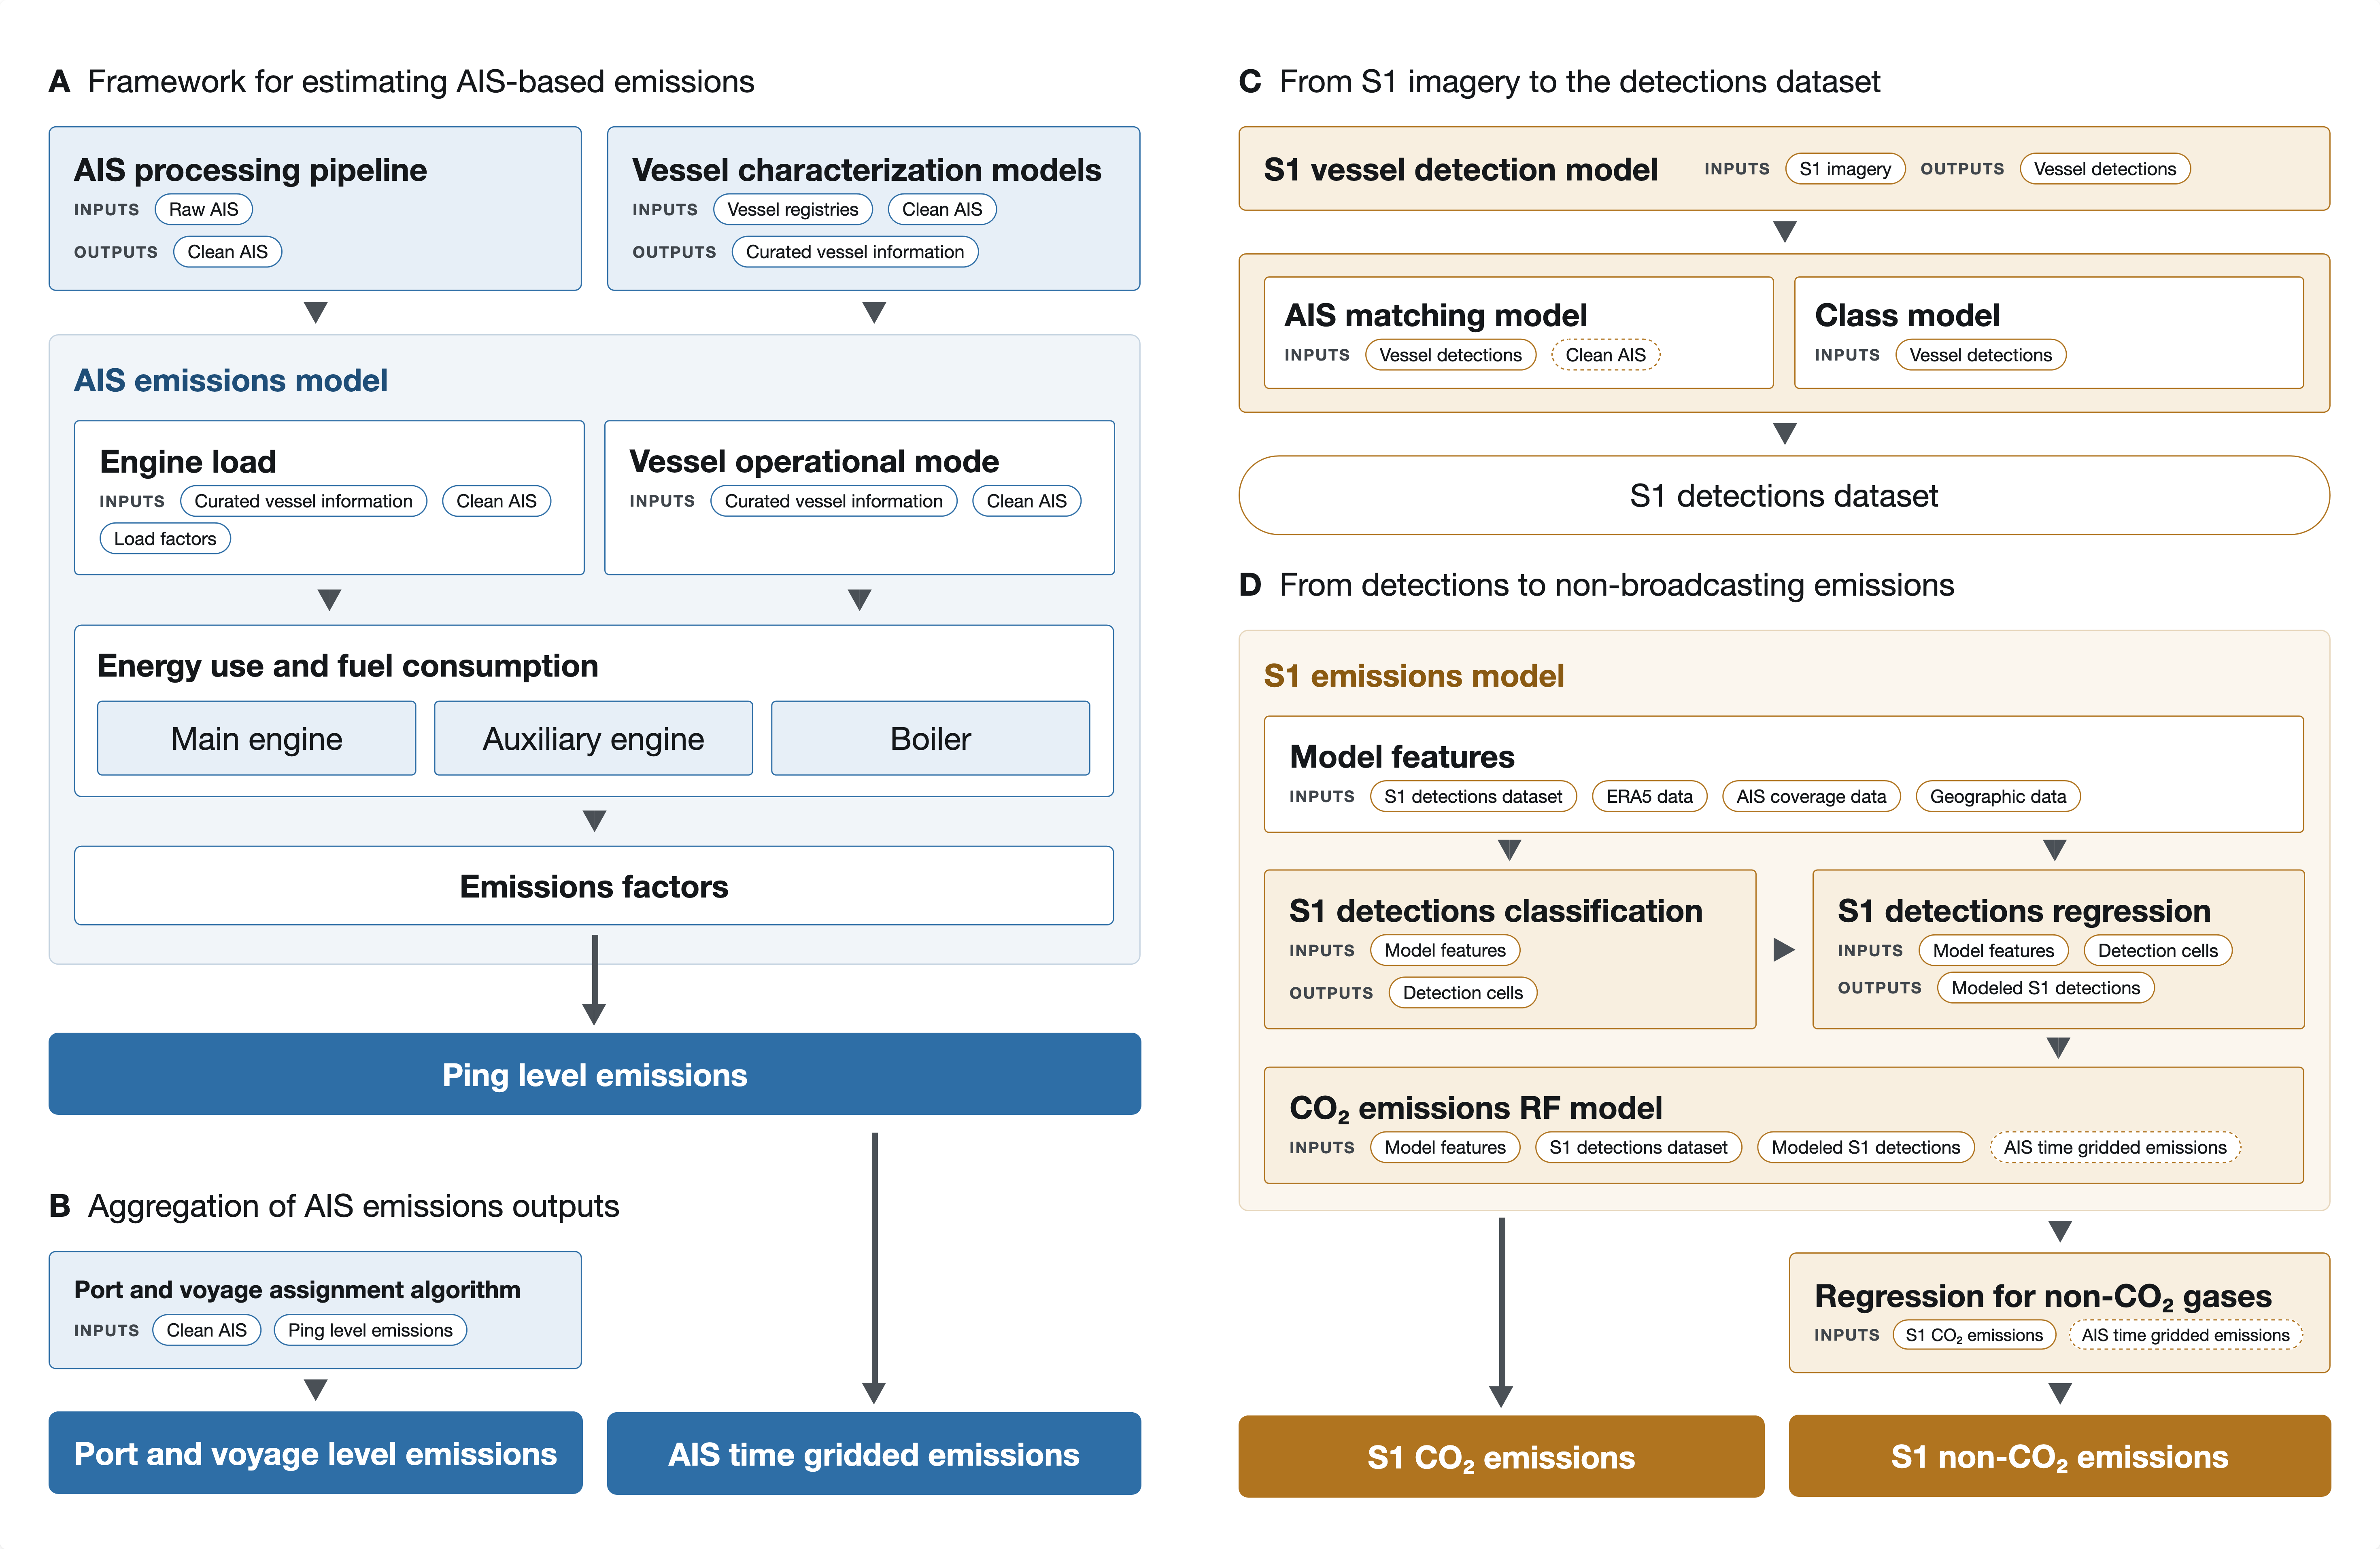
\includegraphics[width=\columnwidth]{figures/fig-framework-flowchart-simpler.png}
    \caption{Conceptual flowchart for estimating emissions using the AIS-based emissions model and the S1-unmatched emissions model.}
    \label{fig:gfw_emissions_framework_flowchart}
\end{figure}

The following sections describe our approaches for AIS-broadcasting vessels and non-broadcasting vessels.

\subsection{AIS-broadcasting vessels}

\subsubsection{AIS data description}

\paragraph{AIS messages, port visits, and voyages}

We use individual AIS messages (pings) from the latest version of GFW’s AIS pipeline (`Version 4'), which parses, cleans, and augments raw AIS data \cite{kroodsma2018tracking}. GFW sources raw AIS from commercial providers of terrestrial, satellite and, from 2022, dynamic AIS (Spire Global), covering both Class A and Class B transponders. Raw broadcasts are parsed and decoded from their encoded format into position messages, carrying location, speed and course, and static and voyage messages, carrying the identifiers and attributes a vessel reports about itself. Positions that are invalid, duplicated, or physically implausible are removed before any downstream processing.

Since pings are grouped into segments using a segmenter \cite{kroodsma2018tracking}, the time for a single ping represents the time since the previous ping in that segment; this value is typically small (the mean value is 0.088 hours and the median value is 0.045 hours, or about 5 minutes and 3 minutes respectively), with virtually all pings representing $<$ 24 hours of activity. Because emissions are estimated over the interval each ping represents, what matters for our estimates is not how many pings have long intervals but how much of the emissions total they carry: 80.7\% of our AIS-based CO$_{2}$ emissions come from pings representing one hour or less of activity, 95.0\% from pings representing 12 hours or less, and effectively all from pings representing less than 24 hours (Fig. \ref{fig:fig-emissions-by-message-hour-threshold}, Table \ref{tab:emissions_by_message_hour_threshold}). The activity associated with individual pings form the basis of our ping-level AIS-based emissions estimates, described below. These AIS messages come from a combination of satellite, terrestrial, and dynamic receivers (described in more detail under the section below `Trends in AIS receiver types' and Supplementary Fig. \ref{fig:fig-annual-emissions-by-ais-receiver-type}, Supplementary Fig. \ref{fig:fig-annual-emissions-by-ais-receiver-type-top-flags}, Supplementary Fig. \ref{fig:fig-co2-emissions-change-map-by-receiver-type})

This dataset also classifies whether a fishing vessel is actively engaged in fishing activities at the ping level \cite{kroodsma2018tracking}. Finally, we leverage GFW's algorithm for detecting port visits \cite{gfw_anchorages_website}, allowing us to aggregate ping-level emissions to the vessel-specific port stays, as well as to vessel-specific port-to-port trips (both international and domestic). 

In all, we analyze AIS data for over 775,000 AIS-broadcasting vessels, across 119 billion individual timestamped AIS messages which are assigned to 14.4 million international trips, 112 million domestic trips, and 96.4 million port visits that occurred between 2017 and 2025.

\begin{figure}[H]
    \centering
    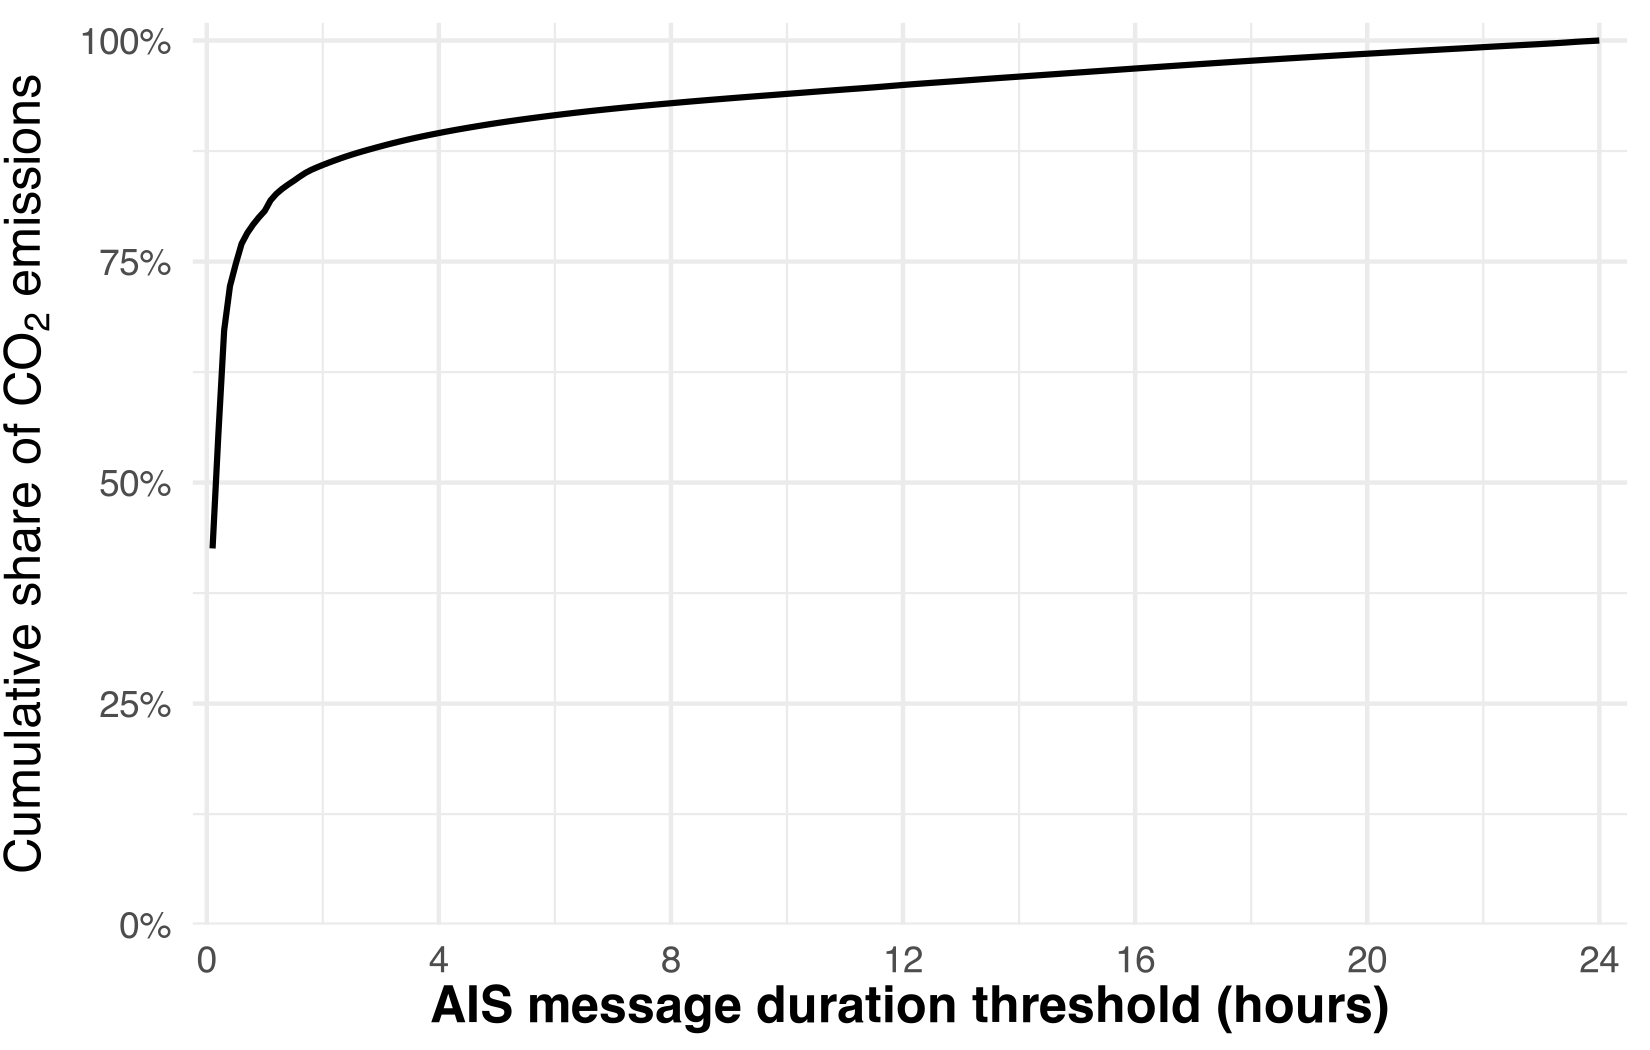
\includegraphics[width=\columnwidth]{figures/fig-emissions-by-message-hour-threshold-1.png}
    \caption{Cumulative share of AIS-based CO$_{2}$ emissions attributable to pings whose assigned interval falls at or below a given threshold (using the full 2017 to 2025 time series of data). Each ping is assigned the time elapsed since the previous ping in its segment, and emissions are estimated over that interval, so long intervals are those over which activity is interpolated across a gap in the message stream rather than observed directly. Values at whole-hour thresholds are given in Table \ref{tab:emissions_by_message_hour_threshold}.}
    \label{fig:fig-emissions-by-message-hour-threshold}
\end{figure}

\begin{table}[!h]
\centering
\caption{\label{tab:emissions_by_message_hour_threshold}Cumulative AIS-based CO$_2$ emissions from messages whose assigned duration falls at or below each whole-hour threshold, 2017 to 2025. Shares are of all AIS-based CO$_2$ emissions, including that from messages with durations longer than 24 hours, so the at-or-below column need not reach 100\%. The above-threshold column is its complement: the share of emissions interpolated across gaps longer than the threshold. Figure \ref{fig:fig-emissions-by-message-hour-threshold} shows the full curve at 0.1-hour resolution.}
\centering
\fontsize{8}{10}\selectfont
\begin{tabular}[t]{rrrr}
\toprule
Threshold (hours) & Cumulative CO$_2$ (million tonnes) & Share at or below & Share above\\
\midrule
1 & 7,086 & 80.73\% & 19.27\%\\
2 & 7,542 & 85.92\% & 14.08\%\\
3 & 7,727 & 88.04\% & 11.96\%\\
4 & 7,859 & 89.53\% & 10.47\%\\
5 & 7,958 & 90.66\% & 9.34\%\\
\addlinespace
6 & 8,036 & 91.55\% & 8.45\%\\
7 & 8,100 & 92.29\% & 7.71\%\\
8 & 8,155 & 92.91\% & 7.09\%\\
9 & 8,203 & 93.46\% & 6.54\%\\
10 & 8,247 & 93.96\% & 6.04\%\\
\addlinespace
11 & 8,291 & 94.46\% & 5.54\%\\
12 & 8,336 & 94.97\% & 5.03\%\\
13 & 8,378 & 95.45\% & 4.55\%\\
14 & 8,419 & 95.92\% & 4.08\%\\
15 & 8,459 & 96.37\% & 3.63\%\\
\addlinespace
16 & 8,499 & 96.83\% & 3.17\%\\
17 & 8,539 & 97.28\% & 2.72\%\\
18 & 8,576 & 97.71\% & 2.29\%\\
19 & 8,612 & 98.12\% & 1.88\%\\
20 & 8,646 & 98.51\% & 1.49\%\\
\addlinespace
21 & 8,679 & 98.88\% & 1.12\%\\
22 & 8,711 & 99.25\% & 0.75\%\\
23 & 8,743 & 99.61\% & 0.39\%\\
24 & 8,777 & 100.00\% & 0.00\%\\
\bottomrule
\end{tabular}
\end{table}

\FloatBarrier

\paragraph{Vessel characteristics data}

Translating AIS vessel activity data into emissions estimates requires information on numerous vessel-specific characteristics including vessel class, main engine power (kW), engine type, gross tonnage, maximum design speed (knots), vessel construction year, and engine operating speed (RPM). A key contribution of this work was therefore to refine and expand GFW's vessel characteristics database to include accurate estimates of these attributes for all 775,000 AIS-broadcasting vessels included in our analysis. For each vessel, this information comes from: (1) official registry information when available \cite{park2023tracking}, or (2) when registry data are unavailable, machine learning vessel characteristics models. We briefly define these models here, and provide full details on training data, features, model performance, and known limitations in the Sections \ref{sec:vessel-characteristics-models} and \ref{sec:vessel-characteristics-numeric-models}.

Leveraging work pioneered by \cite{kroodsma2018tracking}, GFW uses a primary vessel classification model to assign each AIS-broadcasting vessel into one of 32 vessel classes (Section \ref{sec:primary-vessel-class-model}). For vessels classified as `cargo' or `tankers' by GFW's primary vessel classification model, we developed new gradient boosting sub-models that refine the general vessel classification into sub-categories aligned with the Fourth IMO Greenhouse Gas Study vessel class types: five cargo categories (bulk carrier, container, general, refrigerated, and ro-ro) and four tanker categories (oil, chemical, liquefied gas, and other liquids) (Section \ref{sec:cargo-submodel} and \ref{sec:tanker-submodel}). The sub-models are trained on port visit history and vessel activity features, using labels derived from over 26,000 vessels with known IMO vessel class types (S\&P Maritime StatCode5 categories), and achieve weighted F1 scores of 0.91 (cargo) and 0.87 (tanker). These refined cargo and tanker vessel class categories allows us to more accurately assign auxiliary engine power and boiler power to each vessel, which are based on lookup tables according to vessel class and size \cite{fourth2020greenhouse}. 

For the main engine power, gross tonnage, maximum design speed estimates, vessel construction year, and engine operating speed, we develop separate random forest regression models (Section \ref{sec:vessel-characteristics-numeric-models}). All models are trained using the same features: inferred vessel classification scores, AIS self-reported shiptype messages, activity and location features derived from AIS usage, and values inferred from prior regression models. All models were trained on datasets of around 360,000 labeled registry samples, with a holdout test set of 90,000 for an 80/20 train-test split. The main engine power, gross tonnage, maximum design speed, engine RPM, and construction year regression models achieved traditional R$^{2}$ values exceeding 0.92, 0.94, 0.86, 0.53, and 0.45 respectively.

The resulting vessel characteristics dataset contains the necessary metadata for estimating emissions using an AIS-based methodology for over 775,000 active AIS-broadcasting vessels.

It should be noted that even when registries exist, vessel characteristics can be unrepresentative, particularly for fishing vessels. For instance, evidence from the European fishing sector suggests that vessels often use engines larger than those officially registered \cite{EC_EnginePower_2019}, while fraud also extends to reported vessel length and other characteristics \cite{ECA_FisheriesControl_2017}. Underreported main engine power would lead to an underestimation of AIS-based emissions from these vessels; and if underreported main engine power data are used for training models to infer main engine power, this may lead to a systematic underestimation of AIS-based emissions for vessels using inferred main engine power.

\subsubsection{Vessel class and characteristics models}\label{sec:vessel-characteristics-models}

Two families of machine learning models are used to estimate vessel classes and properties. Vessel class is determined by a combination of a broad, primary vessel class model and focused cargo and tanker sub-type models. Vessel properties are determined by six separate models used to estimate the following vessel characteristics: gross tonnage (GT), main engine power (kW), design speed (kn), year-of-build (year), and engine type (class). Random forest classifiers are used for the primary vessel class and the engine subtype, random forest regression models are used to estimate gross tonnage, engine power, design speed, and year of build. Finally, gradient boosting classifiers are used for the cargo and tanker sub-type models. Details about each model can be found in the relevant subsections below.

All models are trained on three categories of features derived from AIS information: inferred features (37), identity features (14), and activity features (13). The cargo and tanker sub-type models are trained on an additional 50 features derived from port visits. These features were built with Word2Vec (50 dimensions, window 10, minimum count 5) over each vessel's sequence of anchorage visits, from high-confidence port visits in the 365 days to 2025-06-01; a vessel's vector is the visit-weighted mean of the anchorages it used. Inferred features consist of vessel class neural network scores and neural network estimates for vessel length, tonnage, engine power, and crew size \cite{kroodsma2018tracking}. Identity features include identification data broadcast through a vessel's AIS, such as the first digit and the broadcast vessel class. Activity features describe patterns in a vessel's AIS activity over time, such as fraction of active hours, average speed, distance from shore, etc.

Training/test data for all models has an 80/20 split, and is stratified by vessel class and the first digit of each MMSI to mitigate bias by vessel type or region. The number of training samples varied for each model as labeled data was available, with the primary GFW vessel class model having the maximum 500,000 total samples. Test sample sizes available for all models are provided in the metrics Table \ref{tab:model-summary}. For each vessel characteristic model, Table \ref{tab:characteristic-availability} summarizes the percentage of vessels that had information already available from public sources, private sources, or for which inferred values from our models were used. 

\begin{table}[htbp]
  \centering
  \small
  \caption{Performance for every model.
  Held-out values use the metric named in the \emph{Metric} column, so rows are comparable within a family but not across families.}
  \label{tab:model-summary}
  \begin{tabular}{@{}llrrcc@{}}
    \toprule
    Model & Target & $n$ train & $n$ test & Metric & Held-out \\
    \midrule
    \multicolumn{6}{@{}l}{\textit{Classification models}} \\
    Vessel class        & 32 classes  & 510\,486  & 127\,645  & macro-F1 & 0.878 \\
    Engine type         & 4 classes  & 46\,108  & 11\,527  & macro-F1 & 0.550 \\
    Cargo sub-type      & 5 classes     & 11\,744 & 2\,939  & macro-F1 & 0.855     \\
    Tanker sub-type     & 4 classes     & 5\,903  & 1\,477  & macro-F1 & 0.712     \\
    \midrule
    \multicolumn{6}{@{}l}{\textit{Regression models}} \\
    Main engine power   & kW            & 13\,842  & 3\,542  & $R^2$    & 0.929 \\
    Gross tonnage       & GT            & 62\,636  & 15\,687  & $R^2$    & 0.944 \\
    Design speed        & knots         & 8\,808  & 2\,241  & $R^2$    & 0.861 \\
    Engine RPM          & rev$/$min     & 45\,868 & 11\,467  & $R^2$   & 0.533 \\
    Construction year   & year          & 45\,868  & 11\,467  & $R^2$    & 0.447 \\
    \bottomrule
  \end{tabular}
\end{table}


\begin{table}[htbp]
  \centering
  \small
  \caption{Availability of vessel characteristics used in emissions modeling, by source.
  ``Inferred'' is the percentage of vessels for which the characteristic were not matched to any registry and was therefore inferred by our machine-learning models. ``Public Sources'' is the percentage sourced from any publicly available registry, including that maintained by IMO's GISIS (Global Integrated Shipping Information System). ``Private Sources'' is the percentage sourced from proprietary vessel databases, chiefly S\&P Global Market Intelligence Ships Dataset and to a smaller extent non publicly available lists maintained by Global Fishing Watch.}\label{tab:characteristic-availability}
  \begin{tabular}{@{}lrrr@{}}
    \toprule
    Characteristic & Inferred (\%) & Public Sources (\%) & Private Sources (\%) \\
    \midrule
    Vessel Class      & 82.5 & 17.5 & 0.0 \\
    Gross Tonnage     & 85.4 & 14.3 & 0.2 \\
    Length            & 89.8 & 6.9  & 3.3 \\
    Main Engine Power & 92.5 & 3.1  & 4.4 \\
    Engine Type       & 93.9 & 0.0  & 6.1 \\
    Year of Build     & 94.0 & 0.0  & 6.0 \\
    Engine RPM        & 95.1 & 0.0  & 4.9 \\
    Design Speed      & 98.2 & 0.0  & 1.8 \\
    \bottomrule
  \end{tabular}
\end{table}
\FloatBarrier

The primary GFW vessel class model, used to predict broad classes such as cargo, tanker, trawler, and gear, identifies the cargo and tanker vessels used in this analysis. Based on those classifications, the cargo and tanker sub-type models further refine those predictions into the more granular classes. Note that roughly 5\% of AIS signals are likely associated with non-vessel objects (such as buoys, offshore structures, FADs, etc). These objects are identified as their own vessel class `gear' by the primary GFW vessel class model, and are excluded from the emissions estimates in this paper. Cargo and tanker sub-type labels are drawn from S\&P Global Maritime records, with StatCode5 levels 2--5 mapped to align with the fourth IMO Greenhouse Gas Study vessel class types, keeping only records that report a single MMSI so each label attaches to one vessel identity.


\subsubsection{Primary GFW vessel class model}\label{sec:primary-vessel-class-model}

\paragraph{Target} 
The primary GFW vessel class model made vessel class predictions at the MMSI level for 1.8M active, AIS-broadcasting vessels. Vessels are assigned a unique class, separated into fishing, non-fishing, and gear, where gear refers to non-vessel AIS-enabled objects.
The final assigned vessel class follows a hierarchy determined by the model’s score for that class, where low-scoring classes get a final assignment at a coarser level. For example, a low-scoring “tanker” might be assigned a final vessel class “non-fishing”.


\paragraph{Training data}
The primary GFW vessel class model makes use of all inferred, identity, and activity features described above. Labels are drawn from clean, aggregated registry data, ensuring that re-used MMSIs and MMSIs with conflicting classes by registry are dropped from training. 
500,000 vessels with aggregated registry information were used to train the model, with a holdout set of 130,000 for testing.


\paragraph{Performance}
The model achieves an accuracy of 98.57\%, with weighted precision, recall, and F1 all at 98.7\%. Macro-averaged precision, recall, and F1 are 87.8\%, 64.8\%, and 71.6\%, respectively. The gap between weighted and macro reflects a class imbalance, with rare classes performing worst.
Cargo and tanker vessels are well-represented in the training data and perform well individually. Cargo achieves an F1 score of 97.0\%, and tanker reaches an F1 score of 95.6\%.

\paragraph{Key predictive features}
The top features are determined using the Gini index, an imperfect but useful measure. Transmitted shiptype unavailable: 0.10, median speed: 0.09, most common AIS class: 0.08, transmitted shiptype cargo: 0.07, neural net passenger vessel score: 0.06, neural net gear score: 0.06, neural net cargo score: 0.05.

\paragraph{Interpretability}
The feature importances are relatively spread out across different training features, with the most indicative feature whether or not the vessel broadcasts a shiptype. This makes sense, as vessel class is gear-dominated, and gear typically does not broadcast a shiptype. Other features, such as median speed, AIS class, and cargo shiptype, indicate a combination of vessel behavior and AIS information itself, while the neural net scores for specific classes show the propagation of one model's predictions into the next.


\paragraph{Overfitting controls and known weaknesses}
The model uses regularized hyperparameters ($n_estimators=300$, $max_depth=35$, $min_samples_leaf=10$, $min_samples_split=20$) rather than an unconstrained forest to balance accuracy against model size. In order to mitigate overfitting or regional bias, the 80/20 slit in the train/test data is stratified by MMSI and MMSI region, and the label-exclusion rules reduce noisy or duplicated MMSI from training. The tight cross-validation variance ($±$0.05\% accuracy across folds) suggests the model isn’t overfit to a particular split.

Despite the training data stratification, high-volume classes such as gear and cargo perform very well, while rarer classes where limited data is available struggle significantly. Larger classes, particularly gear, may be over-classified. Since the model score threshold to mitigate low-scoring, incorrect classifications, some genuinely correctly classified vessels may end up assigned too broad of a label.

As the vessel sub-types models rely on the output of the primary vessel classification model predictions, biases and errors are propagated from this model to the next. This effect similarly happens between the neural net scores and the primary GFW vessel class model.


\subsubsection{Cargo sub-type model}
\label{sec:cargo-submodel}

\paragraph{Target}

One of five cargo sub-types (bulk carrier, container, general cargo, refrigerated cargo, ro-ro cargo), for 186\,689 vessels the primary vessel class model classified as cargo.

\paragraph{Training data}

11\,744 vessels with S\&P registry sub-types: bulk carrier 5\,201; general cargo 3\,200; container 2\,166; ro-ro 1\,100; refrigerated 77.

\paragraph{Performance}

Accuracy 90.5\%; macro-F1 85.5\%; weighted F1 90.5\%. Per-class F1: bulk carrier 94.3, container 93.9, general cargo 84.7, ro-ro 84.6, refrigerated 70.3.

\paragraph{Key predictive features}

Importance is the loss in held-out macro-F1 when a feature is permuted, used in place of the Gini index, which is undefined for the gradient boosting models used here. Anchorage embeddings, 50 dimensions permuted together: 0.220. Vessel class neural network scores, 33 permuted together: 0.157. Top speed (95th percentile): 0.029.

\paragraph{Interpretability}

Vessel class neural network scores form a substantial part of this model's classification skill, indicating it is potentially inherited from the primary model rather than learned from vessel behavior.

\paragraph{Overfitting controls and known weaknesses}

Gradient boosting classifiers with early stopping on a held-out internal validation split, rather than a fixed number of boosting iterations. Unlike the primary model, the train/test split here is stratified by sub-type only rather than by MMSI region, with the split fixed by an MMSI hash so it is stable as data is added.

Refrigerated cargo has 77 training vessels; its F1 of 70.3 is indicative only. Ro-ro and general cargo are the main confusion pair among the well-populated classes: 17\% of ro-ro vessels are predicted as general cargo. General cargo is 27\% of the training set but 66\% of predictions, so the model is likely extrapolating beyond its training mix.

As with the primary model, errors are inherited from it: a vessel it misclassifies is refined against the wrong sub-type vocabulary. Labels exist only for S\&P-registered, single-MMSI vessels, and 4.5\% of training vessels have no port visit features at all.

\subsubsection{Tanker sub-type model}
\label{sec:tanker-submodel}

\paragraph{Target}

One of four tanker sub-types (oil, chemical, liquefied gas, other liquids), for 43\,530 vessels the primary vessel class model classified as tanker.

\paragraph{Training data}

5\,903 vessels with S\&P registry sub-types: oil 2\,664; chemical 2\,015; liquefied gas 1\,188; other liquids 36.

\paragraph{Performance}

Accuracy 87.5\%; macro-F1 71.2\%; weighted F1 87.4\%. Per-class F1: liquefied gas 91.8, oil 88.6, chemical 84.3, other liquids 20.0.

\paragraph{Key predictive features}

Top speed (95th percentile): 0.169. Anchorage embeddings, 50 dimensions permuted together: 0.145. Vessel class neural network scores, 33 permuted together: 0.061. Average distance traveled per trip: 0.030.

\paragraph{Interpretability}

One feature, top speed, carries more importance than any other in either sub-type model. That makes the model easy to explain, but it also means it leans on a single behavioral signal that degrades wherever AIS coverage is patchy.

\paragraph{Overfitting controls and known weaknesses}

Gradient boosting classifiers with early stopping on a held-out internal validation split. As with the cargo model, the train/test split is stratified by sub-type only, and the same label-coverage limits and inheritance of errors from the primary model apply.

Performance for \emph{other liquids} is poor: recall 11.1\%, with 89\% of those vessels predicted as oil. With 45 labeled vessels in total the class does not have enough signal to be separated. Oil and chemical tankers are often confused with each other: 13\% of chemical vessels are called oil and 10\% the reverse. 5.6\% of training vessels have no port visit features at all.


\subsubsection{Other vessel characteristics models}\label{sec:vessel-characteristics-numeric-models}

\paragraph{Targets}

Continuous numeric vessel characteristics - main engine power, gross tonnage, design speed, and construction year - are estimated using random forest regression models, while the categorical engine type value is estimated using a random forest classifier. All models make predictions at the MMSI level for 1.8M active, AIS-broadcasting vessels.

\paragraph{Training data}

All models make use of the inferred, identity, and activity features described above. Labels are drawn from clean, aggregated registry data, ensuring that re-used MMSIs and MMSIs with conflating classes by registry are dropped from training.
The engine power model had a training set of 13,000 samples, the gross tonnage model had a training set of 63,000 samples, the design speed model had a training set of 8,808 samples, the construction year and engine RPM models had a training set of 45,868 samples, and the engine type model had a training set of 46,108 samples.

\paragraph{Performance}
\\
\textit{Engine power model}
\\
The engine power model achieved an R$^2$ of 0.929 with a mean absolute error of 548.71 kW and a mean absolute percentage error of 43.8\%.
\\
\\
\textit{Tonnage model}
\\
The tonnage model achieved an R$^2$ of 0.944 with a mean absolute error of 2,830.15 GT and a mean absolute percentage error of 209.6\%.
\\
\\
\textit{Design speed model}
\\
The design speed model achieved an R$^2$ of 0.861 with a mean absolute error of 0.82 kn and a mean absolute percentage error of 4.9\%.
\\
\\
\textit{Year-of-build model}
\\
The year-of-build model achieved an R$^2$ of 0.447 with a mean absolute error of 6.68 and a mean absolute percentage error of 0.3\%.
\\
\\
\textit{Engine RPM model}
\\
The engine RPM model achieved an R$^2$ of 0.533 with a mean absolute error of 360.56 and a mean absolute percentage error of 33.2\%.
\\
\\
\textit{Engine type model}
\\
Accuracy of 99.08\%; macro-F1 54.6\%; weighted F1 0.991\%. Per class F1: oil 99.5\%, gas 61.7\%, turbine 57.1\%, reciprocating 0.00.

\paragraph{Key predictive features}

\textit{Engine power model}
\\
Average engine power inferred by neural network: 0.535. Top speed (95th percentile): 0.149. Average tonnage inferred by neural network: 0.104.
\\
\\
\textit{Tonnage model}
\\
Average tonnage inferred by neural network: 0.626. Fraction of hours spent at port: 0.0968. Average distance traveled per trip: 0.041.
\\
\\
\textit{Design speed model}
\\
Top speed (95th percentile): 0.609. Median speed: 0.054. Neural network supply vessel score: 0.051.
\\
\\
\textit{Year-of-build model}
\\
Average engine power inferred by the neural network: 0.162. First digit of the MMSI code: 0.101. Average tonnage inferred by the neural network: 0.063.
\\
\\
\textit{Engine RPM model}
\\
Average gross tonnage inferred by the neural network: 0.310. Average length inferred by the neural network: 0.093. Average percentage of self-identified shiptype messages as fishing: 0.074.
\\
\\
\textit{Engine type model}
\\
Top speed (95th percentile): 0.096. Neural network patrol vessel score: 0.080. Average engine power inferred by the neural network: 0.062.

\paragraph{Interpretability}

Both the engine power and the tonnage predictions are largely driven by the neural network's inferred values, indicating that these models are refining existing predictions.
\\
The design speed predictions are most heavily reliant on the vessel's top speed and median speed, which makes intuitive sense as the two act as a proxy for design speed.
\\
The year-of-build predictions are less singularly reliant on one strong signal, but are driven the most by the neural network's inferred engine power and the first digit of the MMSI code. The latter likely acts as a proxy for build/registration era for each flag state.
\\
The engine RPM predictions are largely weighted by physical characteristics of the vessel, but similarly less reliant on a single feature. The physical characteristics describing a vessel likely act as a proxy for RPM, while the self-identified shiptype likely distinguishes fishing and non-fishing vessel properties.
\\
The top features for engine type predictions are much more diffuse, suggesting that no single feature strongly separates engine types and the model relies on combinations of weaker signals.

\paragraph{Overfitting controls and known weaknesses}
To mitigate overfitting, all models are trained with a fixed random seed and a train/test split stratified by vessel class and first-digit MMSI. The engine type model additionally used class-weight balancing to counteract severe class imbalance in the training labels. However, because the engine type labels are so heavily skewed towards oil engines, the model only performs reliably for that class, and semi-reliably for gas. As higher volume data becomes available for a greater diversity of engine types, future models will be more sophistication and better predictive of the less represented types. 

The year-of-build model has a 6-7 year mean error, suggesting that it is useful for predicting general build era up to around a decade, but not reliable for year-by-year predictions. The engine RPM model has mean error of 360 revolutions per minute, indicating that it can capture very broad patterns but with more relative error than the year-of-build model.
The engine power, tonnage, and design speed models all show the same pattern: performance is strongest in the mid-range of each variable and degrades substantially at the extremes, where training data is sparse.

\subsubsection{Emissions model for AIS-broadcasting vessels}

We adapted our AIS-based model from the methodologies described in the 2017 ICCT study on global shipping emissions \cite{olmer2017greenhouse} and the 2020 IMO Fourth Greenhouse Gas Study \cite{fourth2020greenhouse}, making modifications to better align with the structure and characteristics of our data sets. From a high-level, we: 

1. Determine the main engine energy use, auxiliary engine energy use, and boiler energy use for each individual AIS message based on dynamic vessel movement and static vessel characteristic data

2. Determine fuel consumption for each individual AIS message based on dynamic vessel movement and static vessel characteristic data.

3. For the seven pollutants whose emissions factors depend on energy use (CH$_{4}$, CO, N$_{2}$O, NO$_{x}$, VOCs, PM$_{2.5}$, and PM$_{10}$), multiply the engine and boiler energy use numbers by pollutant- and engine-type-specific emissions factors in order to determine the amount of emissions for each pollutant associated with the engines and boiler for each ping.

4. For the two pollutants whose emissions factors depend on fuel consumption (CO$_{2}$ and SO$_{x}$), for each ping multiply the fuel consumption by the appropriate pollutant- and engine-type-specific emissions factors in order to determine the amount of emissions for each pollutant and ping.

5. Add up the emissions for each of the nine pollutants, from across the engines and boiler, to obtain the total emissions for each ping and each of these nine pollutants. 

We focus our analysis purely on estimating emissions associated with fuel combustion in the main engine, auxiliary engine, and boiler; we do not include  methane slip on vessels that use liquefied natural gas, or other non-combustion fugitive emissions associated with refrigeration, cooling, or venting of VOCs from vessels that transport liquid cargo such as oil and chemicals.

Main engine energy use is estimated based on the time between each AIS ping (hours), the main engine power from the vessel characteristics dataset, and a load factor used to adjust the estimate. The load factor is the product of four coefficients: (1) a weather correction factor (represented by distance to shore, a proxy that can be observed from AIS data - vessel operating beyond 5 nautical miles from shore receive a value of 1.15; vessels operating within 5 nautical miles receive a value of 1.1 \cite{fourth2020greenhouse}); (2) a hull fouling correction factor, which causes resistance in the water (set at 1.07 according to \cite{olmer2017greenhouse}); and (3) a vessel draft correction factor (set at 0.85, the emissions-weighted average draft correction factor from \cite{fourth2020greenhouse}; and (4) a cubic term of vessel speed divided by  the vessel's maximum design speed. To determine the vessel speed associated with each AIS message, we use either: 1) the transmitted instantaneous speed associated with the AIS message if less than an hour has passed since the last message was transmitted; or 2) the implied speed for messages for which more than an hour has passed since the previous message (calculated as the distance traveled divided by the elapsed time between the two messages). We apply this hierarchy since implied speed can be imprecise for short time intervals between pings due to signal latency; meanwhile, instantaneous speed can be unrepresentative of longer time intervals between pings, in which case implied speed is more representative. Following \cite{coello2015ais, sala2018economics}, for fishing vessels we adjust the main engine load factor so that it falls between 0.2 and 0.9, and assign a main engine load factor of 0.75 to trawlers and dredge fishing vessels that are actively fishing due to the energy intensive nature of their fishing operations. 

In accordance with \cite{fourth2020greenhouse}, our model also accounts for differences in auxiliary engine power energy use and boiler energy use depending on the vessel type, as well as the vessel’s operational phase—whether it is at berth, at anchor, maneuvering, or at sea. These phases are identified using AIS speed, distance to port, and distance to the coast. Power outputs for auxiliary engines and boilers, based on vessel class and size, are extracted from \cite{fourth2020greenhouse} and are applied accordingly for each phase. 


Fuel consumption, for each of the main engine, auxiliary engine, and boiler engine, are next calculated as energy use multiplied by specific fuel consumption (SFC). The SFC for each of the main engine, auxiliary engine, and boiler engine are based on engine type and fuel type  \cite{fourth2020greenhouse}. Our vessel characteristics database includes broad categories of engine type (oil, gas, or turbine), as well as engine operating speed which allows us to differentiate between high speed diesel, medium speed diesel, and low speed diesel. Since our vessel characteristics database does not specify fuel type for each vessel, we use the average values from across fuel types for each type of engine. For the main engine, SFC is further modulated based on engine load: engines operating at low loads below 20\% operate inefficiently, and therefore consume more fuel for the same amount of energy output  \cite{olmer2017greenhouse, fourth2020greenhouse}. For the two pollutants whose emissions factors depend on fuel use (CO$_{2}$ and SO$_{x}$), these emissions are therefore directly adjusted during inefficient low load operation.


For the other seven pollutants whose emissions factors depend instead directly on energy use (CH$_{4}$, CO, N$_{2}$O, NO$_{x}$, VOCs, PM$_{2.5}$, and PM$_{10}$), we account for inefficient main engine operation during low load by using the low load correction factors provided by \cite{epa2020ports} (which were subsequently adopted by \cite{fourth2020greenhouse}). Low-load correction factors are provided in the EPA report as a table showing a range from $\le 2\%$ through $\ge 20\%$ in incremental steps of 1\%. To use these, we apply the following hierarchy: if our estimated main engine load is $\le 2\%$, we apply the correction factor corresponding to $\le 2\%$ if our estimated main engine load is greater than $\ge 20\%$, we apply a correction factor of 1; if our estimated main engine load corresponds perfectly to one of the incremental percentage steps in the table, we apply the corresponding  correction factor; finally, if if our estimated main engine load falls between two values in the table, we linearly interpolate between the correspond correction values. We are therefore able to determine and apply an appropriate low-load correction factor for all AIS messages and all pollutants.

After calculating energy use, we apply pollutant-specific emission factors to the main engine, auxiliary engine, and boiler for each of the three GHGs and six pollutants, following \cite{olmer2017greenhouse, fourth2020greenhouse}. CO$_{2}$ and SO$_{x}$ emissions factors are based on fuel use (e.g., are represented in units of grams of pollutant per gram of fuel); CH$_{4}$, CO, N$_{2}$O, NO$_{x}$, VOCs, PM$_{2.5}$, and PM$_{10}$ emissions factors are based on energy use (e.g., are represented in units of grams of pollutant per killowatt-hour). Again, since we have information for each vessel on engine type but not on fuel type, we take average values for the emissions factors for each engine type from across the appropriate fuel type options. NOx emissions factors additionally depend on the vessel’s IMO engine Tier, which is determined by year of build and engine RPM (both of which are included in our database of estimated vessel characteristics). To get total emissions for each AIS message (i.e., emissions from the previous ping in a segment to the current one), we sum emissions from both engines and boilers.

Starting January 1, 2020, the IMO mandated a low sulfur fuel switch, reducing the allowable sulfur content from 3.5\% to 0.5\% \cite{imo_sulphur_2020}. To account for this, we adjust the emissions factors for SO$_{x}$, as well as for PM$_{2.5}$ and PM$_{10}$ (which are partially produced by sulfur), using the sulfur content of fuel for each period \cite{fourth2020greenhouse}. The SO$_{x}$ fuel-based emissions factor is calculate using an equation that scales linearly with fuel sulfur percentage content \cite{fourth2020greenhouse}. For pre-2020 data, we estimate this emissions factor based on an assumed global average sulfur content of 2.5\% \cite{olmer2017greenhouse}. Assuming the sulfur content drops from 2.5\% to 0.5\% starting in 2020, we re-calculate the SO$_{x}$ emissions factor for post-2020 using this post-2020 sulfur content. Although these emissions factors do not explicitly account for non-compliance, scrubbers, or low sulfur areas, this 80\% drop of the estimated emissions factor between pre-2020 to post-2020 is consistent with several studies that looked at the impact this new requirement had on global sulfur emissions \cite{yuan2024abrupt, yoshioka2024warming}. PM energy-based emissions factors are based on an equation that uses sulfur fuel content and also depends on SFC \cite{fourth2020greenhouse}, and we again assume an 80\% drop in sulfur content in 2020. We apply these adjusted emissions factors for all SO$_{x}$, PM$_{2.5}$, and PM$_{10}$ emissions starting in January 1, 2020.

\subsubsection{Validating AIS-based emissions model}\label{sec:ais-model-performance}

We use two distinct emissions datasets for validation, one to assess the impact of updated vessel metadata from our random forest models on performance, and another to evaluate the model’s overall performance using emissions associated with actual vessel activity.

\paragraph{Registered data validation}

We have access to a confidential registered dataset of vessels' main engine fuel consumption measured during sea trials over a 24-hour period at a given speed, along with each vessel’s main engine power and design speed. Because these consumption values are not associated with specific trips that can be matched to our trip-level emissions estimates, direct comparison of derived emissions is not possible. However, this dataset allows us to validate the emissions generated by the main engine model module and assess the impact of updated metadata from our random forest models. Specifically, we compare the performance of the main engine model emissions estimates using main engine power and design speed values from the original IMO lookup table \cite{fourth2020greenhouse}  compared with those obtained when using our vessel-specific random forest model predictions of main engine power and design speed. Furthermore, we define the performance ceiling achievable through improved vessel metadata by testing the model with the actual engine power and design speed recorded in the registered dataset.

For a validation sample of 15,679 vessels, we ran the main engine model to calculate main engine energy use, incorporating the weather correction factor for offshore navigation along with the other default hull-fouling and draft correction factors from our main model, over a 24-hour period at the consumption speed provided in the registered dataset. We test three different sets of vessel metadata. For each set, main engine power and design speed were taken from either: (1) Table 81 lookup values from \cite{fourth2020greenhouse}; (2) our vessel-specific random forest model predictions; or (3) the registered dataset. Main engine energy use was then converted to emissions using the same CO$_{2}$ emission factor as in our main model. Since the registered dataset provides vessel-specific main fuel consumption values and not actual emissions values, we converted the registered fuel consumption to emissions by applying a fuel-to-CO$_{2}$ conversion factor of 3.12 (kg CO$_{2}$/tonne fuel), derived from the heavy fuel oil (HFO) and marine diesel oil (MDO) factors weighted by their contribution to global fuel consumption, as reported in \cite{fourth2020greenhouse}. This finally allows us to assess the performance of our model-estimated CO$_{2}$ emissions to those from the registered dataset.

This comparison shows that the updated vessel metadata using random forest models substantially improves model performance compared to that achieved using the original \cite{fourth2020greenhouse} vessel metadata, bringing the results closer to the model performance ceiling.

\begin{figure}[H]
    \centering
    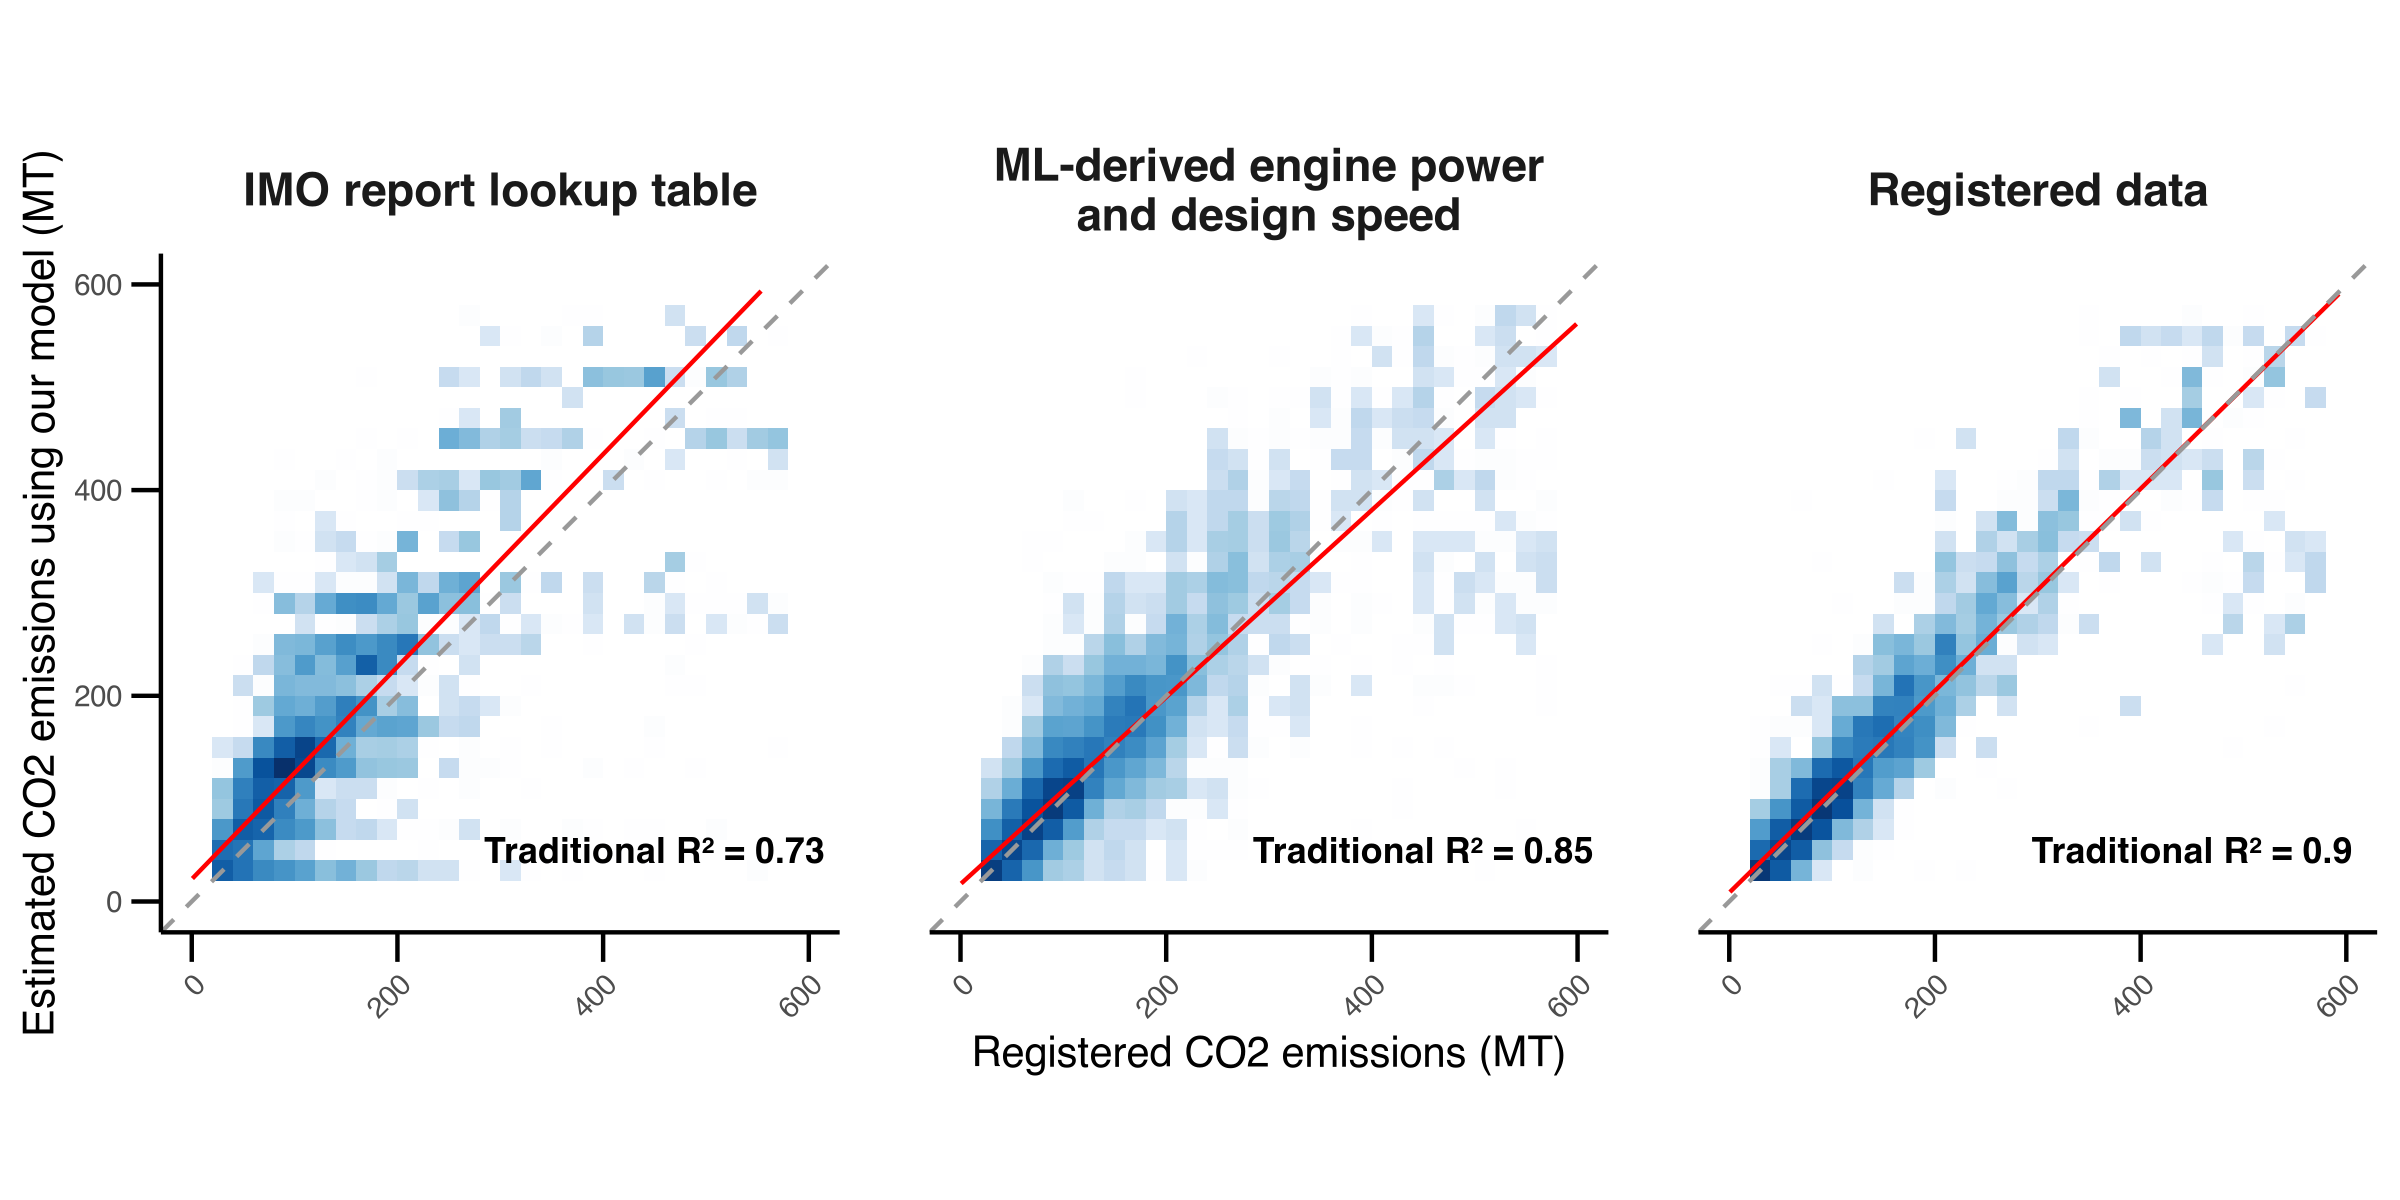
\includegraphics[width=\columnwidth]{figures/fig-registered-data-performance-1.png}
    \caption{Comparison of daily vessel-level CO$_{2}$ emissions estimated using our model with registered emissions from a proprietary vessel database (based on main engine fuel consumption over 24 hours). Estimates are shown using main engine power and design speed from IMO (left), our machine learning random forest models (center), and the same registered dataset (right). The dashed line represents the 1:1 line. Performance values for traditional R$^{2}$ are shown for each set of vessel characteristics. Over 15,000 vessels are represented in the figure, and blue shading indicates point density. All data are rule-of-three compliant, meaning each cell (20×20 mt) displayed contains at least three vessels.}
    \label{fig:fig-registered-data-performance}
\end{figure}

\paragraph{EU MRV data validation}

We also validate our CO$_{2}$ emissions model results against public emissions data from the European Maritime Safety Agency’s Monitoring, Reporting, and Verification (MRV) program  \cite{mrv_emissions}. The MRV dataset provides yearly aggregated emissions—including CO$_{2}$ from main engines, auxiliary engines, gas turbines, boilers, and inert gas generators—along with hours at sea, and distance traveled for each vessel, covering voyages within, from, or to European Economic Area (EEA) “ports of call,” during which cargo is loaded/unloaded or passengers embark/disembark. It excludes port calls for refueling, supplies, crew changes, and similar activities.

Our AIS-derived emissions dataset does not contain detailed information on vessel activity while in port (i.e., whether or not cargo is loaded/unloaded or passengers embark/disembark), making it difficult to determine the exact same trip start and end points as defined in the MRV data, as well as which trips are included in the MRV records for a given year and vessel. To align vessel yearly activity across datasets, we: (1) filter our trip-level emissions data to include only trips that begin and/or end in EEA countries; (2) aggregate these trip-level emissions to annual emissions for each vessel; (3) apply varying matching tolerance margins to the MRV-reported annual hours at sea and select vessels-year from our dataset within these limits, in order to ensure that the trips we use for comparison have a total hours at sea roughly equal to that reported in the MRV dataset; and (4) compare annual MRV emissions with the annual sum of our trip-level emissions for the same vessel and year to evaluate model performance.

\begin{table}[!h]
\centering
\caption{\label{tab:tab-performance-tolerance-table}Performance summary across different thresholds for the hours at sea tolerance between datasets. Results are shown using the R$^{2}$ (measuring linear association between observed and predicted values) and traditional R$^{2}$ (proportion of variance explained compared to the mean-only baseline).}
\centering
\fontsize{8}{10}\selectfont
\begin{tabular}[t]{r|l|r|r}
\hline
Tolerance & Number of vessels & R$^{2}$ & Traditional R$^{2}$\\
\hline
0.05 & 921 & 0.78 & 0.77\\
\hline
0.10 & 1,594 & 0.79 & 0.78\\
\hline
0.15 & 2,274 & 0.80 & 0.80\\
\hline
0.20 & 2,910 & 0.77 & 0.76\\
\hline
0.25 & 3,598 & 0.78 & 0.77\\
\hline
0.30 & 4,373 & 0.71 & 0.67\\
\hline
0.35 & 5,254 & 0.72 & 0.64\\
\hline
0.40 & 6,298 & 0.72 & 0.58\\
\hline
\end{tabular}
\end{table}

\FloatBarrier

In Table \ref{tab:tab-performance-tolerance-table}, performance peaks at a traditional R$^{2}$ of 0.84 for vessels whose times at sea in our dataset are within 15\% of the MRV-reported values (validation sample of 27,657 vessel-year observations, shown in Fig. \ref{fig:fig-mrv-performance}). Beyond this threshold, performance declines as discrepancies grow between our annual aggregated trip activity and that recorded in the MRV dataset.


\begin{figure}[H]
    \centering
    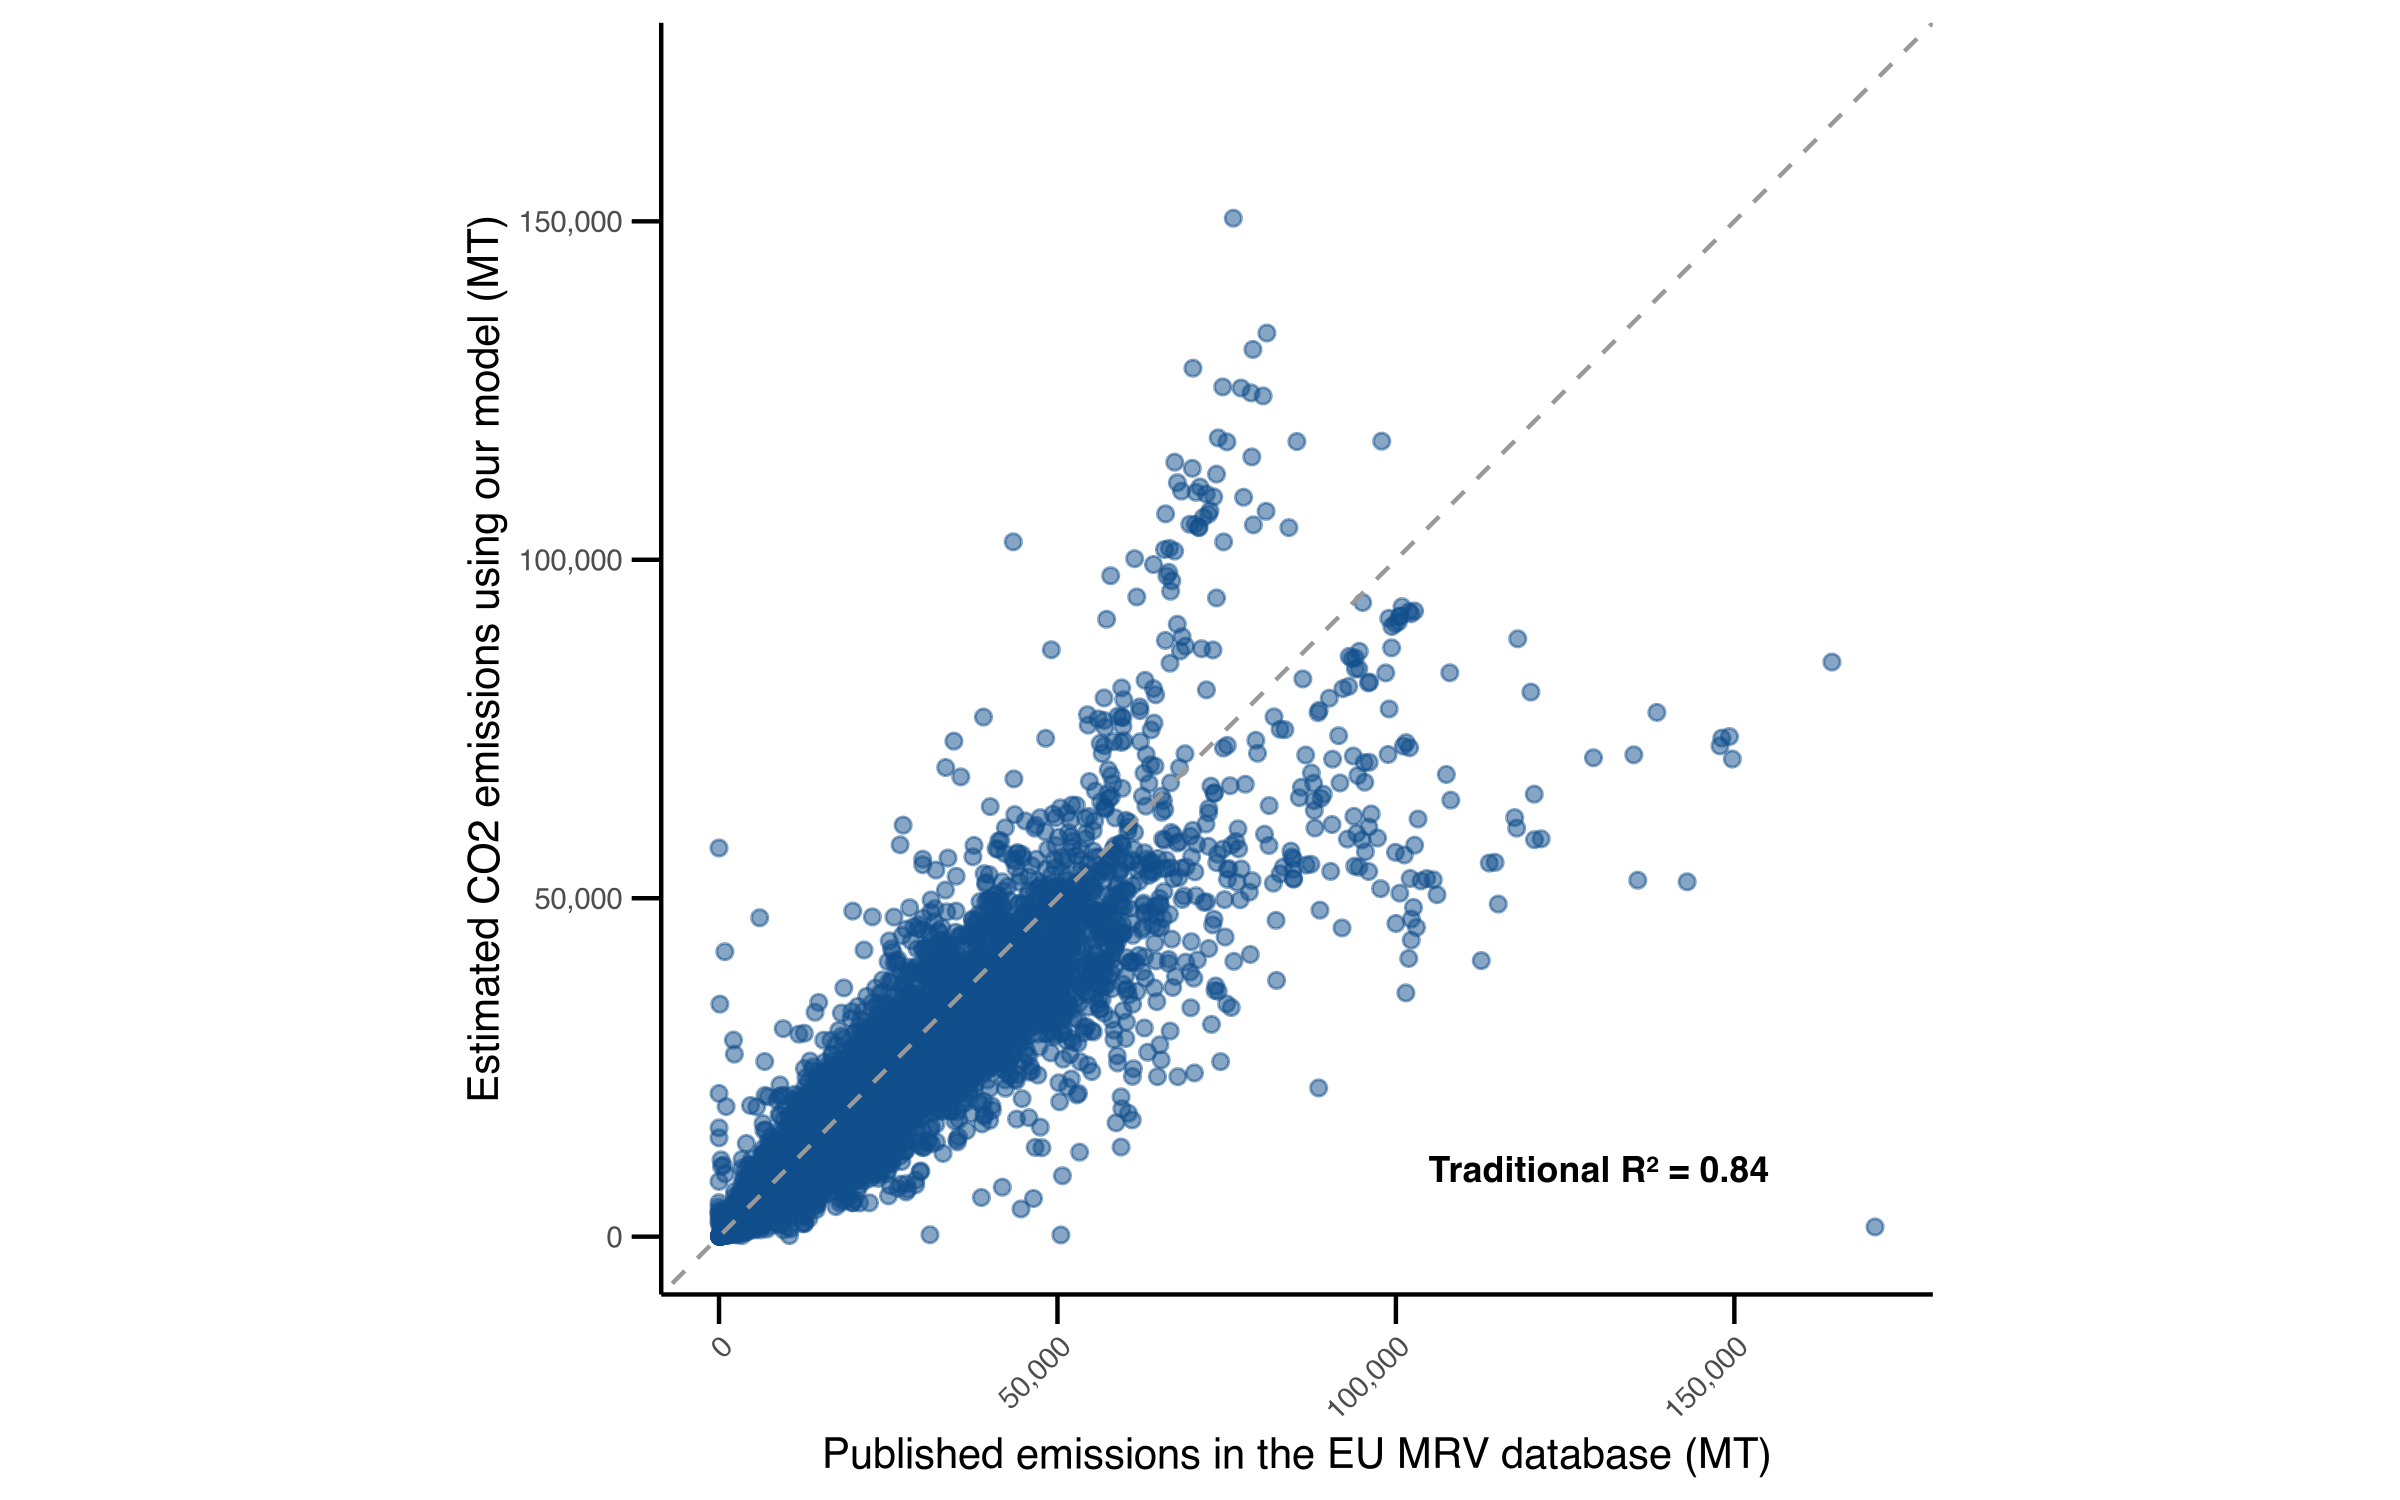
\includegraphics[width=\columnwidth]{figures/fig-mrv-performance-1.png}
    \caption{Comparison of annual vessel-level CO$_{2}$ emissions estimated using our model with published emissions from the EU MRV database. The sample includes 27,657 observations from yearly aggregated vessel trips where hours at sea differ by no more than 15\% between our data and the MRV dataset. The dashed line represents the 1:1 line.}
    \label{fig:fig-mrv-performance}
\end{figure}

\subsection{Non-broadcasting vessels}\label{sec:non-broadcasting-vessels}

\subsubsection{Sentinel-1 SAR data description}

For our S1-unmatched emission estimates, we leverage GFW vessel detections from S1 Synthetic Aperture Radar (SAR) imagery \cite{paolo2024satellite}. The data filtering involved in the GFW vessel detections include removing detections within a 1-km buffer from the shoreline to reduce false positives from land-based objects due to inaccurately defined and dynamic coastlines, repeated detections of potentially fixed objects such as offshore infrastructure, detections from icy areas, moving vehicles close to shore, and other radar ambiguities \cite{paolo2024satellite}. In addition, we also remove detections from known vessel anchorages \cite{gfw_anchorages_website}. Non-vessel fishing gears are too small to be detected from Sentinel-1 SAR imagery, and thus no special filtering is necessary to remove these from the dataset. Vessels detected at anchorage may or may not be active and actually emitting, so we limit our S1-unmatched emissions estimation to focus only on those vessels that are away from anchorage and actively operating in the open water. As a result, we used a dataset containing 31.9 million vessel detections from 2017 to 2025, of which 14.9 million detections were not matched to an AIS-broadcasting vessel (referred to as `S1-unmatched'; the matching process is described in next paragraph). These detections come from across more than 924,000 individual S1 scenes (Fig. \ref{fig:fig-map-fraction-months-imaged}, Fig. \ref{fig:fig-s1-coverage-time-series}).

\begin{figure}[H]
    \centering
    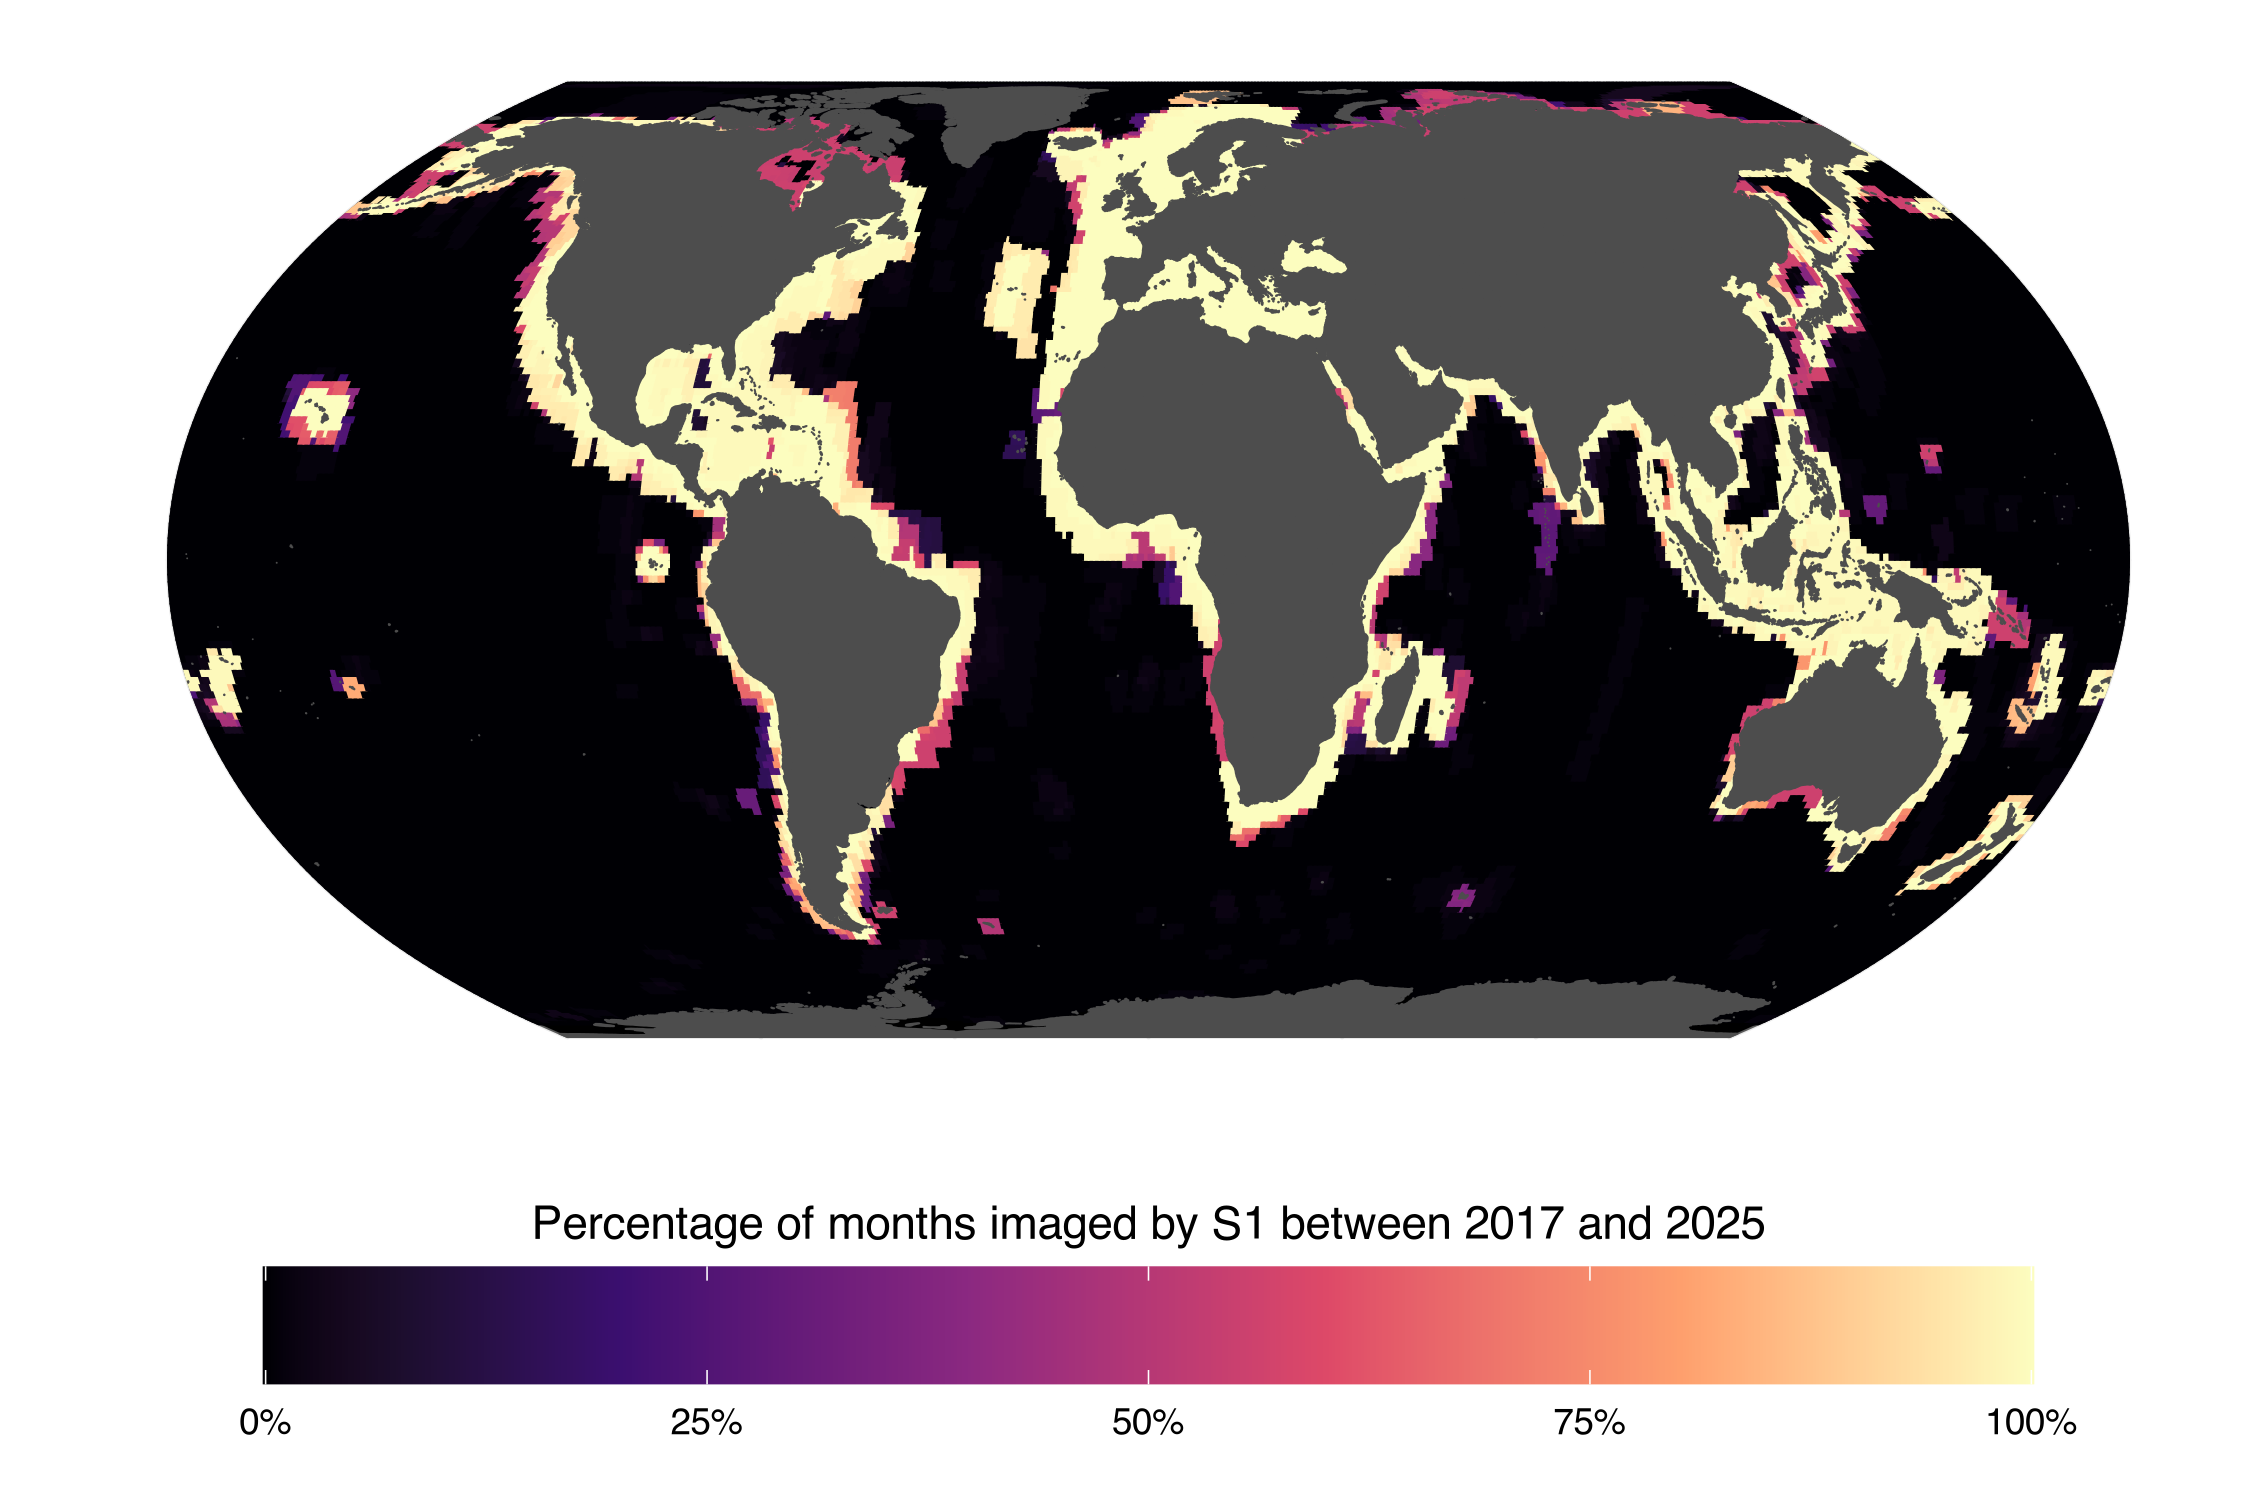
\includegraphics[width=\columnwidth]{figures/fig-map-fraction-months-imaged-1.png}
    \caption{Map showing the percentage of months from 2017 through 2025 that were imaged by S1 for each 1x1 degree pixel.}
    \label{fig:fig-map-fraction-months-imaged}
\end{figure}


\begin{figure}[H]
    \centering    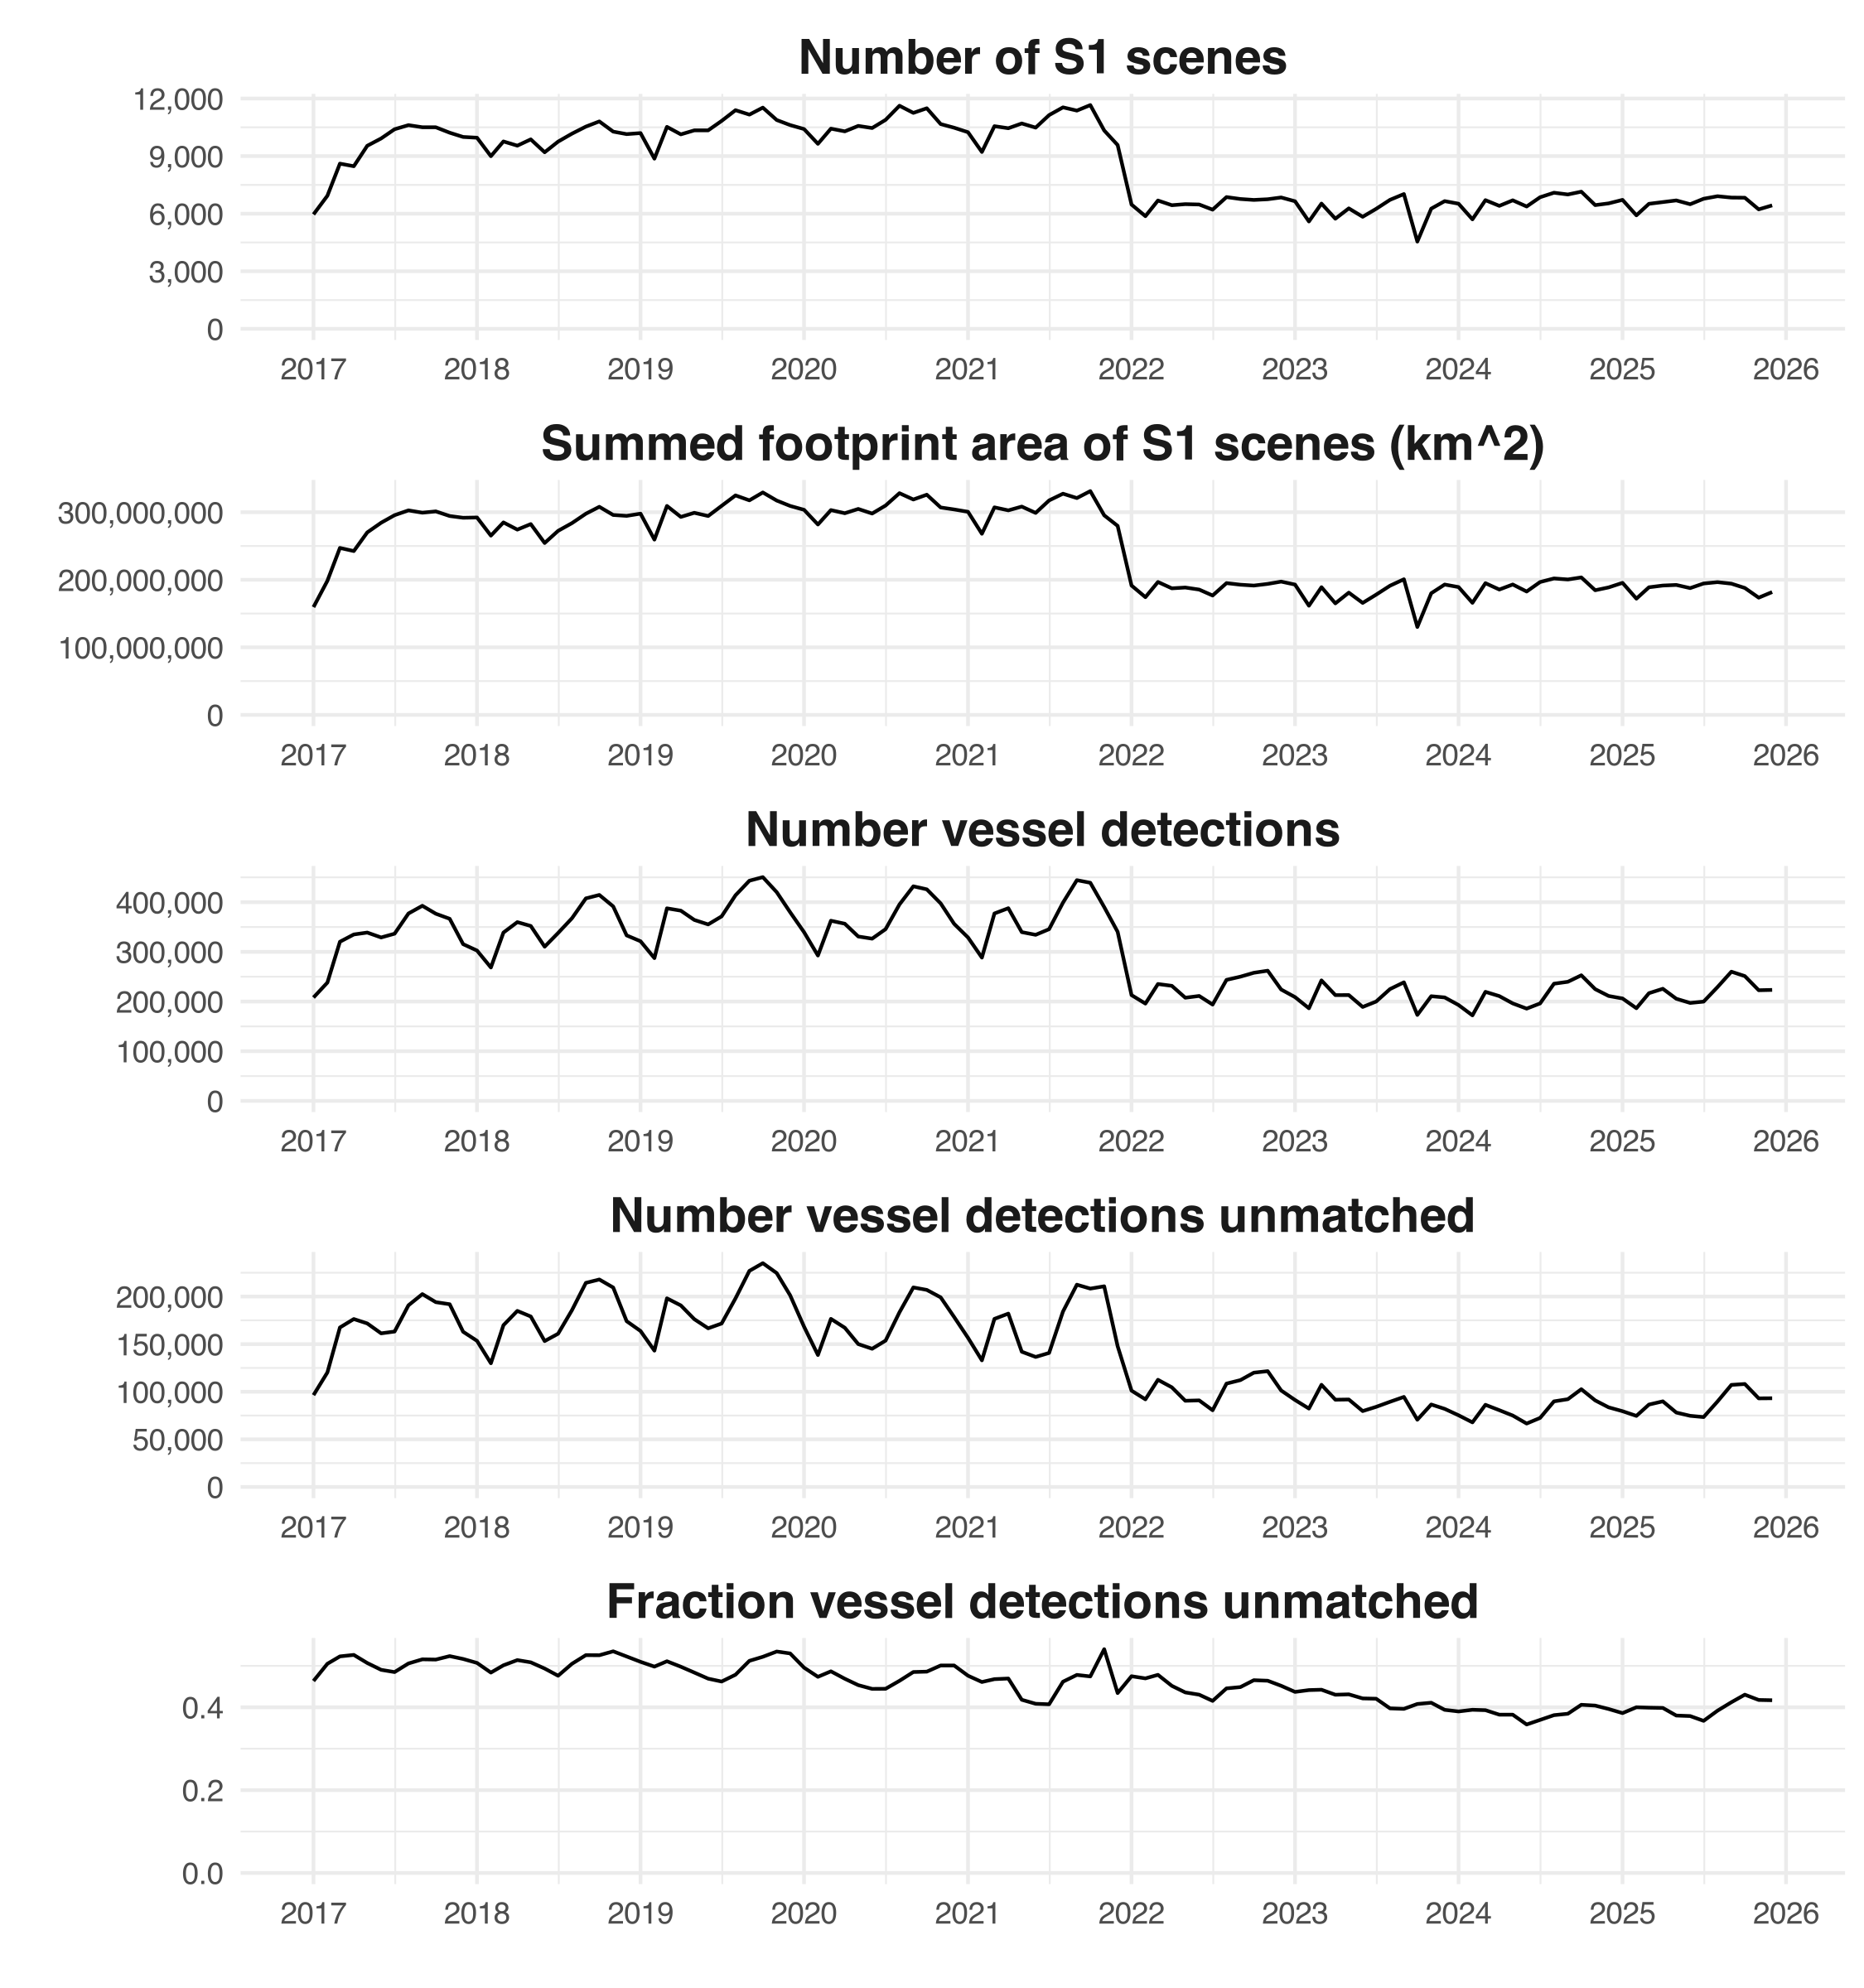
\includegraphics[width=\columnwidth]{figures/fig-s1-coverage-time-series-1.png}
    \caption{Monthly statistics of global S1 coverage including total number of S1 scenes, total imaged area summed across all S1 scenes (which counts each revisit to a given area separately), total number of vessel detections, total number of vessel detections that could not be matched to an AIS-broadcasting vessels, and fraction of the total number of vessel detections that could not be matched to an AIS-broadcasting vessels.}
    \label{fig:fig-s1-coverage-time-series}
\end{figure}

For each vessel detection, the dataset provides its inferred vessel length and likelihood of being classified as either a fishing vessel or non-fishing vessel. By spatiotemporally matching AIS-broadcasting vessels to S1 detections, the dataset also categorizes each vessel detection as either being matched to an AIS-broadcasting vessel (`matched'), or being unmatched to an  an AIS-broadcasting vessel (`unmatched') \cite{kroodsma2022revealing,paolo2024satellite}. Importantly, although `unmatched' detections may often correspond to vessels that does not use AIS at all, it does not necessarily mean the vessel does not carry AIS - it could still carry AIS, but its transmission may be experiencing a gap for a variety of transmission or reception reasons. The detection-AIS matching utilizes a probabilistic framework that produces matching scores representing the likelihood of detection-AIS pairs being correct, and global threshold of the matching score \cite{kroodsma2022revealing,paolo2024satellite}. The matching considers AIS positions before and after the detection timestamp up to 12 hours away, and larger AIS position gaps typically result in lower matching scores with candidate detections. Therefore, an unmatched detection in this study may correspond to either a vessel not equipped with AIS or a vessel equipped with AIS but experiencing a transmission gap. The transmission gap can be intentional or a result of poor AIS reception. A broadcasting vessel that goes unmatched in this way therefore erroneously has its emissions counted in both our `AIS-based' and `S1-unmatched' estimates, inflating our fused total. To estimate the extent of this double counting and its effect on our fused emissions estimates, we first use a hold-out experiment in which S1 detections with high-confidence AIS matches were re-matched using our matching algorithm but with AIS positions withheld within a window of the detection timestamp. This gives the probability that a detection of a broadcasting vessel is missed by the matching as a function of the AIS transmission gap; this rises gradually from 6.8\% at a 2-hour gap to 27.4\% at 8 hours and 45.4\% at 18 hours (Fig. \ref{fig:fig-s1-matching-double-counting}a). Second, because each AIS message represents the interval since the vessel's previous message, we know how much of our AIS-based CO$_{2}$ is emitted during gaps of each length (Fig. \ref{fig:fig-emissions-by-message-hour-threshold}, Fig. \ref{fig:fig-s1-matching-double-counting}b). Multiplying the two gives the share of AIS-based emissions emitted during gaps in which a detection of the vessel would have been missed, which we call the share at risk of double counting: 5.1\% (Fig. \ref{fig:fig-s1-matching-double-counting}c-d, Table \ref{tab:s1_matching_double_counting_by_gap}). Because S1 images a vessel at an arbitrary moment, this share is also the probability that any given detection of a broadcasting vessel is missed. Our 17.0 million matched detections are therefore the 94.9\% that were not missed, and the remaining 0.92 million detections of broadcasting vessels sit among our 14.9 million unmatched detections, where they make up 6.2\% of the total. Our S1-unmatched emissions are estimated from the density of unmatched detections, so a missed broadcasting vessel contributes to them like any other unmatched detection, and about 6.2\% of S1-unmatched emissions (171 million tonnes over 2017 to 2025, or 1.5\% of our combined total) therefore duplicate emissions already included in our AIS-based estimate. Finally, the missed detections are also absent from the matched detections used to train the emissions regression model, which raises the emissions it assigns to each detection by 5.4\%.  Upwards of 11.9\% of our S1-unmatched emissions may therefore be due to double-counting from missed matches during AIS transmission gaps; this translates to 2.8\% of our total fused emissions (Table \ref{tab:s1_matching_double_counting_summary}). 

\begin{figure}[H]
    \centering
    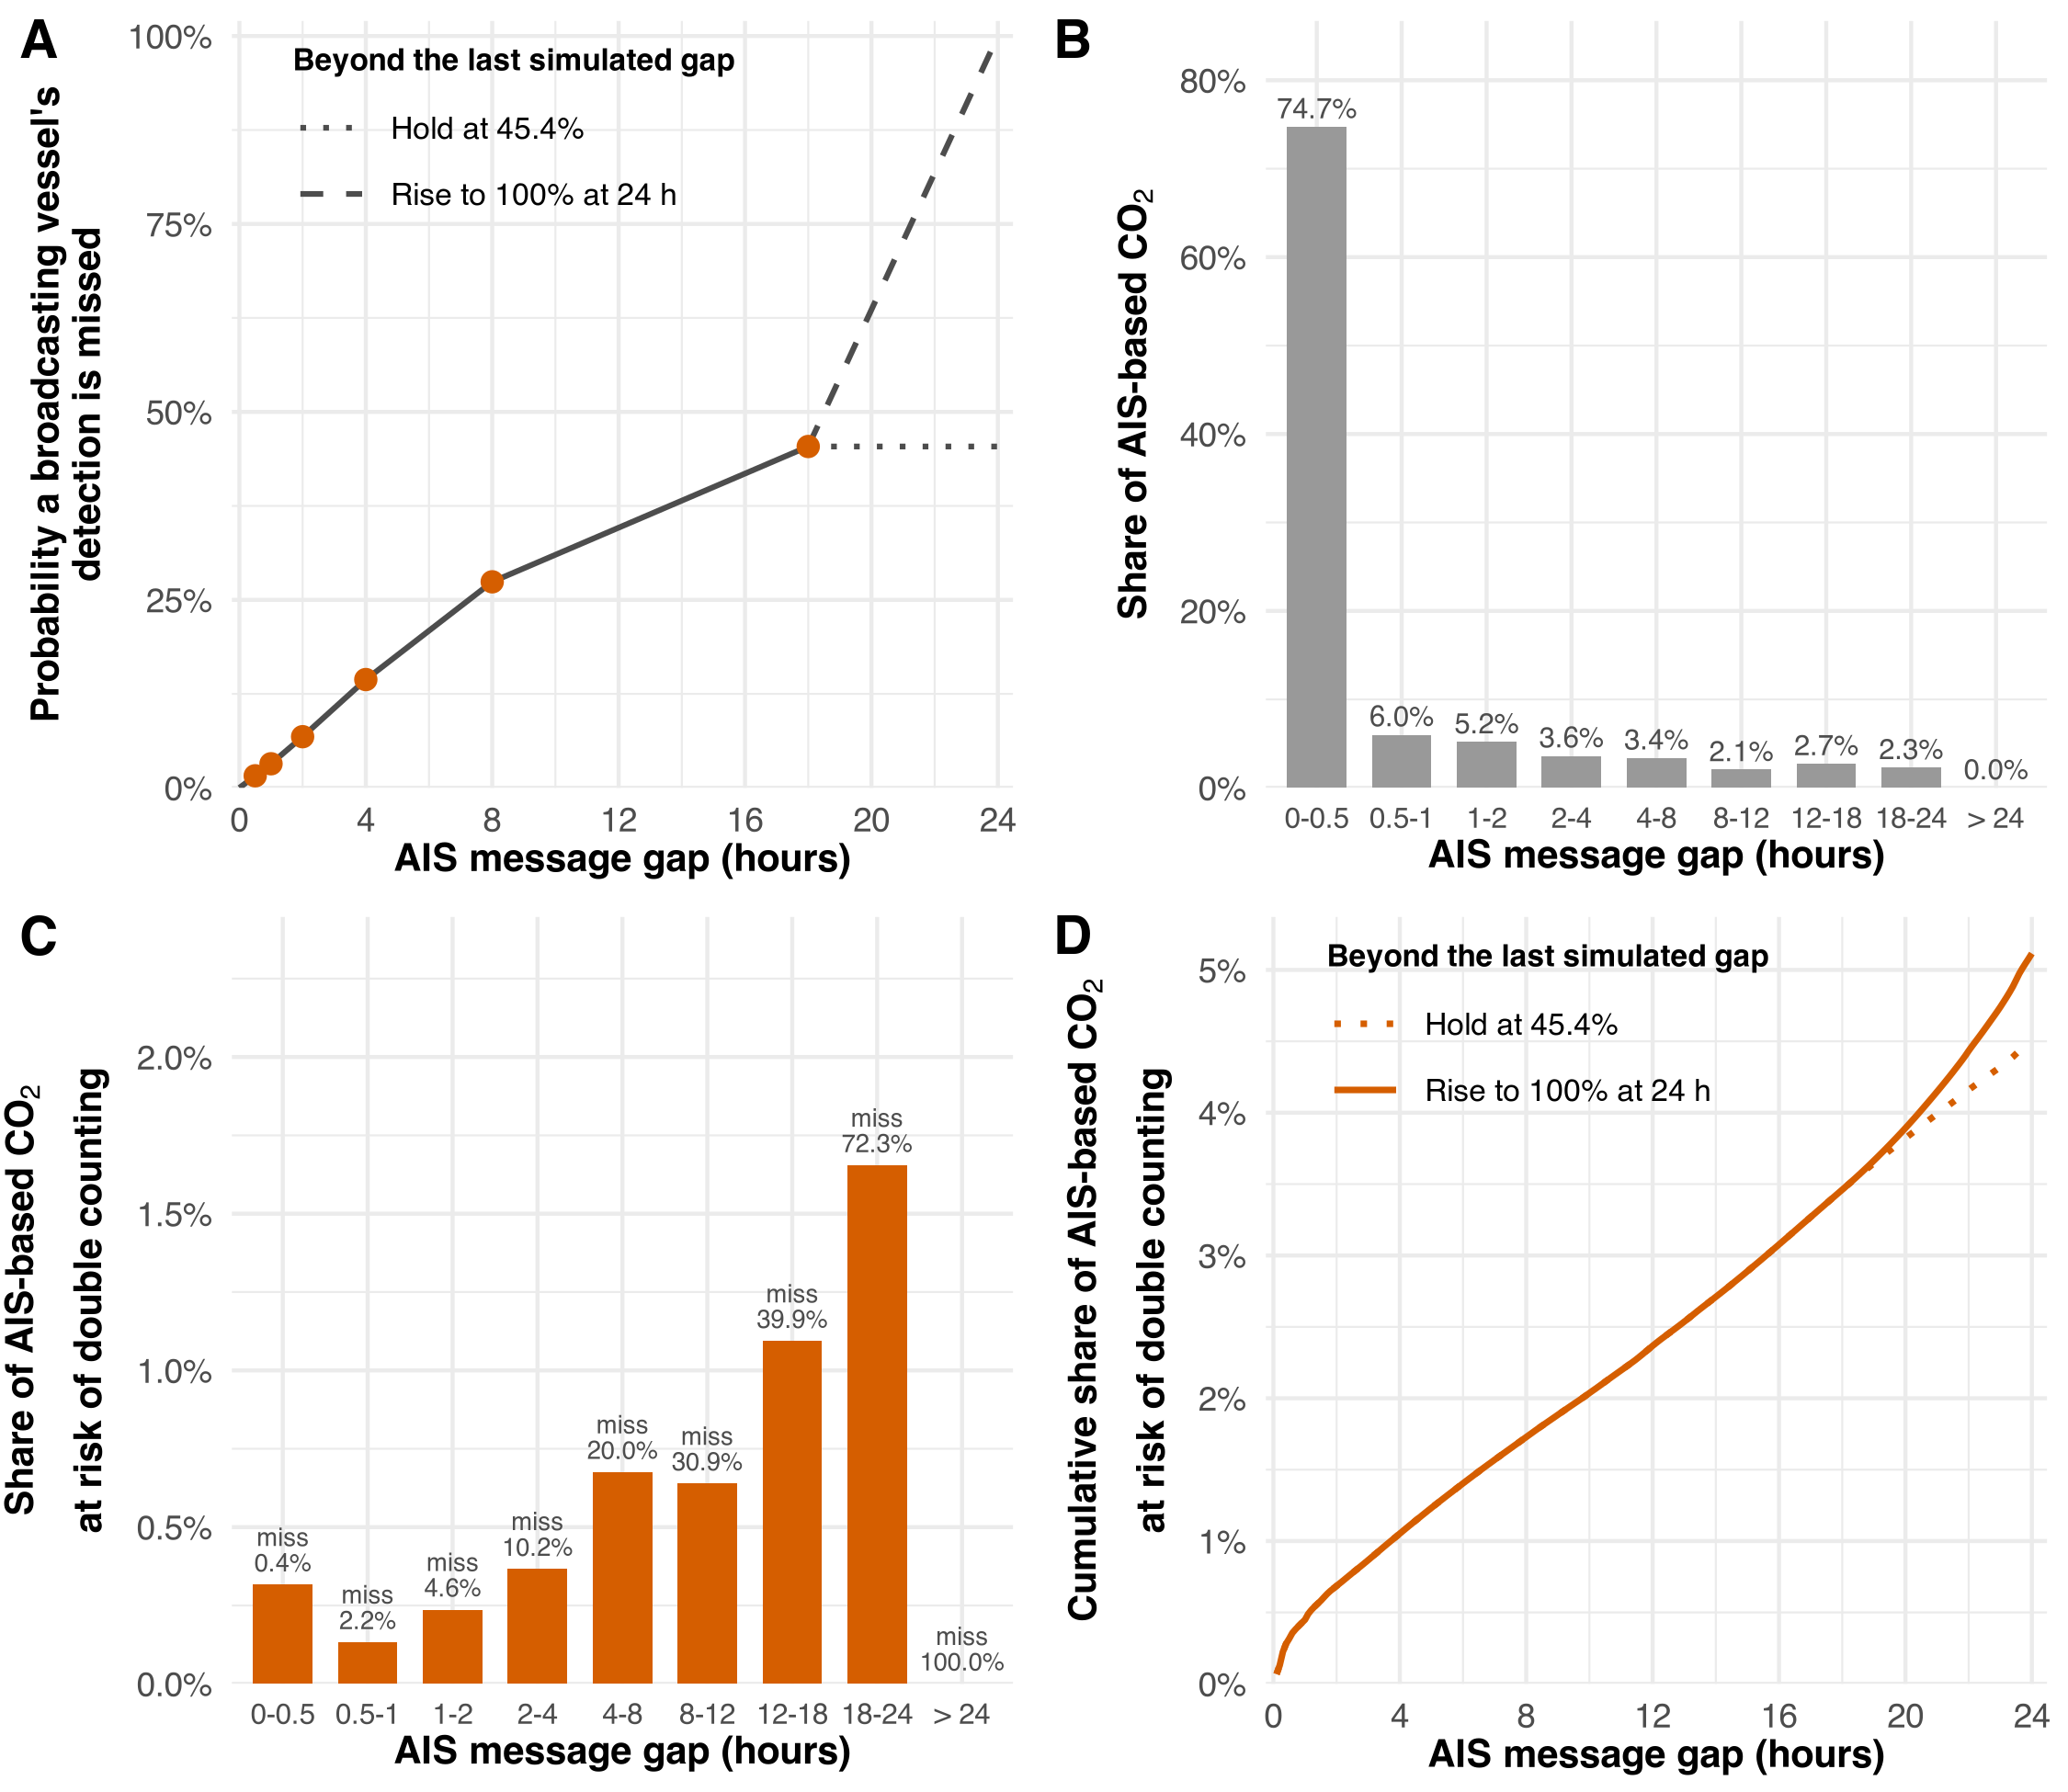
\includegraphics[width=\columnwidth]{figures/fig-s1-matching-double-counting-1.png}
    \caption{(a) Probability that a detection of an AIS-broadcasting vessel is missed by the matching, by the length of the gap in its AIS messages. Beyond the last simulated gap, we assume the line either reaches 100\% at the 24-hour matching window (dashed) or stays flat (dotted). (b) Share of AIS-based CO$_{2}$ emissions, 2017 to 2025, by the length of the AIS gap during which they were emitted. (c) B multiplied by A, the share of AIS-based emissions at risk of double counting: emitted during gaps in which a detection of the vessel would have been missed and counted as S1-unmatched. The miss probability for each bin is labeled above the bar. (d) Cumulative total of C; the end point is the 5.1\% in the text.}
    \label{fig:fig-s1-matching-double-counting}
\end{figure}

\begin{table}[!h]
\centering
\caption{\label{tab:s1_matching_double_counting_by_gap}AIS-based CO$_2$ emissions by the length of the AIS message gap they were emitted in, 2017 to 2025, and the share of each at risk of double counting: the emissions in the bin multiplied by the probability, from GFW's hold-out matching experiment, that an S1 detection made during a gap of that length fails to match and is counted as unmatched. The miss rate is interpolated between the simulated gaps and taken to rise to 100\% at 24 hours, the width of the matching window; messages representing more than 24 hours are treated as always missed. Figure \ref{fig:fig-s1-matching-double-counting} shows the inputs and the cumulative curve; Table \ref{tab:s1_matching_double_counting_summary} carries the totals through to emissions.}
\centering
\fontsize{8}{10}\selectfont
\begin{tabular}[t]{lrrrr}
\toprule
AIS message gap (hours) & Share of AIS-based CO$_2$ & Miss rate (emissions-weighted) & Share at risk of double counting & Cumulative share at risk\\
\midrule
0-0.5 & 74.73\% & 0.4\% & 0.32\% & 0.32\%\\
0.5-1 & 6.00\% & 2.2\% & 0.13\% & 0.45\%\\
1-2 & 5.19\% & 4.6\% & 0.24\% & 0.69\%\\
2-4 & 3.61\% & 10.2\% & 0.37\% & 1.05\%\\
4-8 & 3.37\% & 20.0\% & 0.68\% & 1.73\%\\
\addlinespace
8-12 & 2.07\% & 30.9\% & 0.64\% & 2.37\%\\
12-18 & 2.74\% & 39.9\% & 1.09\% & 3.46\%\\
18-24 & 2.29\% & 72.3\% & 1.65\% & 5.12\%\\
> 24 & 0.00\% & 100.0\% & 0.00\% & 5.12\%\\
\bottomrule
\end{tabular}
\end{table}

\begin{table}[!h]
\centering
\caption{\label{tab:s1_matching_double_counting_summary}Double counting between the AIS-based and non-broadcasting CO$_2$ estimates, 2017 to 2025, following the steps in the text. The share at risk is the total of Table \ref{tab:s1_matching_double_counting_by_gap}; because S1 images a vessel at an arbitrary moment, it is also the probability that a detection of a broadcasting vessel is missed by the matching. The matched detections are the ones that were not missed, which gives the number missed and their share of the unmatched detections. Non-broadcasting emissions are estimated from unmatched detections, so that share of them duplicates AIS-based emissions. The last two rows add the effect of the missed detections being absent from the matched detections the emissions regression model is trained on. The miss rate beyond 18 hours is taken to reach 100\% at 24 hours (Fig. \ref{fig:fig-s1-matching-double-counting}A, dashed).}
\centering
\fontsize{8}{10}\selectfont
\begin{tabular}[t]{>{\raggedright\arraybackslash}p{8cm}r}
\toprule
  & Value\\
\midrule
Share of AIS-based CO$_2$ at risk of double counting: emitted during AIS gaps in which a detection of the vessel would be missed & 5.1\%\\
Matched S1 detections & 17.0 million\\
Detections of broadcasting vessels missed by the matching & 0.92 million\\
Unmatched S1 detections & 14.9 million\\
Share of unmatched detections that are broadcasting vessels & 6.2\%\\
\addlinespace
Non-broadcasting CO$_2$ that duplicates AIS-based CO$_2$, 2017--2025 & 175 million tonnes (1.5\% of combined total)\\
Increase in the emissions per detection fitted by the emissions regression model, because the missed detections are absent from its training data & 5.4\%\\
Upper bound on non-broadcasting CO$_2$ that duplicates AIS-based CO$_2$, including that increase & 11.9\% of non-broadcasting CO$_2$ (2.9\% of combined total)\\
\bottomrule
\end{tabular}
\end{table}

\FloatBarrier

\subsubsection{Overview of S1-unmatched emissions modeling framework}

Here we describe our model for estimating S1-unmatched emissions at a 1x1-degree gridded resolution with global coverage, consistently each month from 2017 through 2025, and disaggregated by vessel type (fishing or non-fishing). A common limitation in SAR-derived inventories is the sparse temporal coverage of Low Earth Orbit satellites, where dynamic vessel movements are inadequately captured by discrete, fixed-time overpasses. To directly addresses this spatial-temporal mismatch, we avoid assuming a steady-state temporal vessel activities from snapshots of imagery. Instead, we estimate S1-unmatched emissions using a multi-model framework that uses a combination of AIS-derived emissions, S1 vessel detections, and additional spatiotemporal model features. Let's first consider the case of modeling S1-unmatched CO$_2$ emissions. For the first model, we build a regression random forest to predict AIS-based CO$_2$ emissions using matched S1 detection density and additional spatiotemporal model features (subsequently referred to as the 'emissions regression' model). We can then use this model to predict S1-unmatched CO$_2$ emissions using unmatched S1 detection density (i.e., detections not matched to an AIS-broadcasting vessel). Because this model requires data for both AIS-based emissions and S1 detections, it is trained using data from pixel-month observations that are imaged by S1 (Fig. \ref{fig:fig-map-fraction-months-imaged}). For pixel-month observations that are imaged by S1, we can use the directly observed unmatched S1 detection density for this prediction. 

Not all pixel-month observations are imaged by S1, either because there were simply no S1 overpasses in a given area and month, or because a given area is completely outside the S1 footprint (Fig. \ref{fig:fig-map-fraction-months-imaged}). For these observations without S1 imaging, we interpolate unmatched detection density using a two-stage hurdle framework which is composed of two models: (1) a classification random forest that predicts the presence or absence of unmatched detections (subsequently referred to as the 'detection classification' model); and (2) a regression random forest regression to estimate the density of unmatched detections, conditional on there being any detections present  (subsequently referred to as the 'detection regression' model). Therefore, for pixel-months not imaged by S1, we can use the predicted density of unmatched detections from the 'detection regression' model as an input to the 'emissions regression' model in order to predict the amount of S1-unmatched CO$_2$ emissions in these areas.


To reduce overall model complexity, we use a more simplified approach for estimating S1-unmatched emissions for the other eight gases (the other two GHGs and six pollutants). With our AIS-based emissions model, emissions of all gases are calculated using gas-specific emissions factors that linearly convert either fuel consumption or engine energy use (killowatt-hours) to emissions (with energy use being closely correlated to fuel consumption). Emissions of all non-CO$_2$ gases are therefore highly correlated with CO$_2$ emissions (although there are some non-linearities: for example ,different vessel types and sizes have different emissions factors for auxillary engine and boiler energy use; we apply correction factors for some pollutants when engines are operating at very low loads; the 2020 IMO low sulfur policy affects emissions factors of some pollutants but not others). Therefore, rather than training nine separate random forest models to predict emissions for each of the nine gases, we simplify the overall modeling framework by building a single random forest to predict CO$_2$ emissions and then eight linear regression models to predict emissions of each gas from the emissions of CO$_2$. Each of these linear models is composed of five coefficients. To account for the temporal discontinuity that occurs when the 2020 IMO low sulfur policy was implemented, we include a post-2020 dummy variable. To account for the fact that fishing and non-fishing vessels have slightly different emissions profiles, we interact the post-2020 dummy variable with a dummy variable for fishing/non-fishing  such that regression coefficients are estimated separately for pre- and post-2020 periods for both fishing and non-fishing vessels (yielding four separate coefficients). Finally, to account for the fact that there are spatial patterns in terms of where vessels of different sizes are located, and that different size vessels have different emissions profiles, we include a coefficient for $log(distance to shore + 1)$. 

\begin{align*}
\text{emissions}_{\text{gas},i} = {} 
  & \beta_1 \times \text{emissions}_{\text{CO}_2,i} \times \text{post2020}_{\text{FALSE}} \times \text{fishing}_{\text{FALSE}} \\
  & + \beta_2 \times \text{emissions}_{\text{CO}_2,i} \times \text{post2020}_{\text{TRUE}} \times \text{fishing}_{\text{FALSE}} \\
  & + \beta_3 \times \text{emissions}_{\text{CO}_2,i} \times \text{post2020}_{\text{TRUE}} \times \text{fishing}_{\text{TRUE}} \\
  & + \beta_4 \times \text{emissions}_{\text{CO}_2,i} \times \text{post2020}_{\text{TRUE}} \times \text{fishing}_{\text{TRUE}} \\
  & + \beta_5 \times \text{emissions}_{\text{CO}_2,i} \times \log(\text{distance\_to\_shore} + 1) + \epsilon_i
\end{align*}

Therefore, for all non-CO$_2$ gases, we first predict S1-unmatched CO$_2$ emissions using the framework above, and then convert these emissions to non-CO$_2$ S1-unmatched emissions using these eight linear models. Pollutant-to-CO$_2$ ratios were evaluated with distance to shore winsorized at the 0.1st percentile of the fitting distribution (442 m), to avoid extrapolating the log-linear ratio below the support of the data, where it can become negative.

In the sections below, we detail: 1) the unit of observation and outcome variable for each of the three models; 2) the features used in each of the three models; 3) the data pre-processing steps used for each model; 4) the performance testing procedures and results for each model; 5) the feature importance results for each model; and 6) the final prediction procedure for obtaining our global spatiotemporal S1-unmatched emissions estimates.

\subsubsection{Units of observation and outcome variables}

\paragraph{Emissions regression} The observation unit for predicting emissions is the total emissions (of a given GHG or pollutant) in a given 1x1 degree ocean pixel, in a given month, for a given type of vessel (either non-fishing or fishing). For model training, we used the emissions estimated from the AIS-based model, extracting ping-level emissions from broadcasting vessels that occurred in ocean water beyond a 1 km buffer from shore, which corresponds to the spatial coverage of S1 detections processed by GFW and therefore excludes inland waterways, lakes, rivers, and ports. These ping-level emissions were aggregated to our unit of observation (by 1x1 degree pixel, month, and fishing/non-fishing vessel types), and observations with zero AIS-based emissions were excluded. Emissions for each observation are aggregated across all vessel sizes. 

For the random forest to predict CO$_2$ emissions, in order to capture the vessel length distribution of S1 detections across different vessel sizes, for each observation we include several model features that represent the number of S1 detections in each of several vessel length bins. For non-fishing vessels, we use 10 length bins: 0-25m, 25-50m, ..., 200-225m, and 225+ m;  for fishing vessels, which are typically smaller, we use five length bins: 0-25m, 25-50m, 50-75m, 75-100m, and 100+ m (Fig. \ref{fig:fig-length-bin-distributions}). We use length bins because length is representative of main engine power (Fig. \ref{fig:fig-ais-length-power-relationship}), which is directly related to emissions in our AIS-based model. We stratify by vessel type (fishing or non-fishing) because they have significantly different length size distributions (Fig. \ref{fig:fig-length-bin-distributions}), and also because some fishing vessel types have fundamentally different emissions profiles than non-fishing vessels (i.e., trawlers and dredgers emit more at low speeds due to the nature of their energy-intensive gear deployment, which is reflected in their gear-specific main engine load factor adjustment.) Additionally, because emissions are highly right-skewed, we log-normalize the CO$_2$ emissions as the dependent variable. 

\begin{figure}[H]
    \centering
    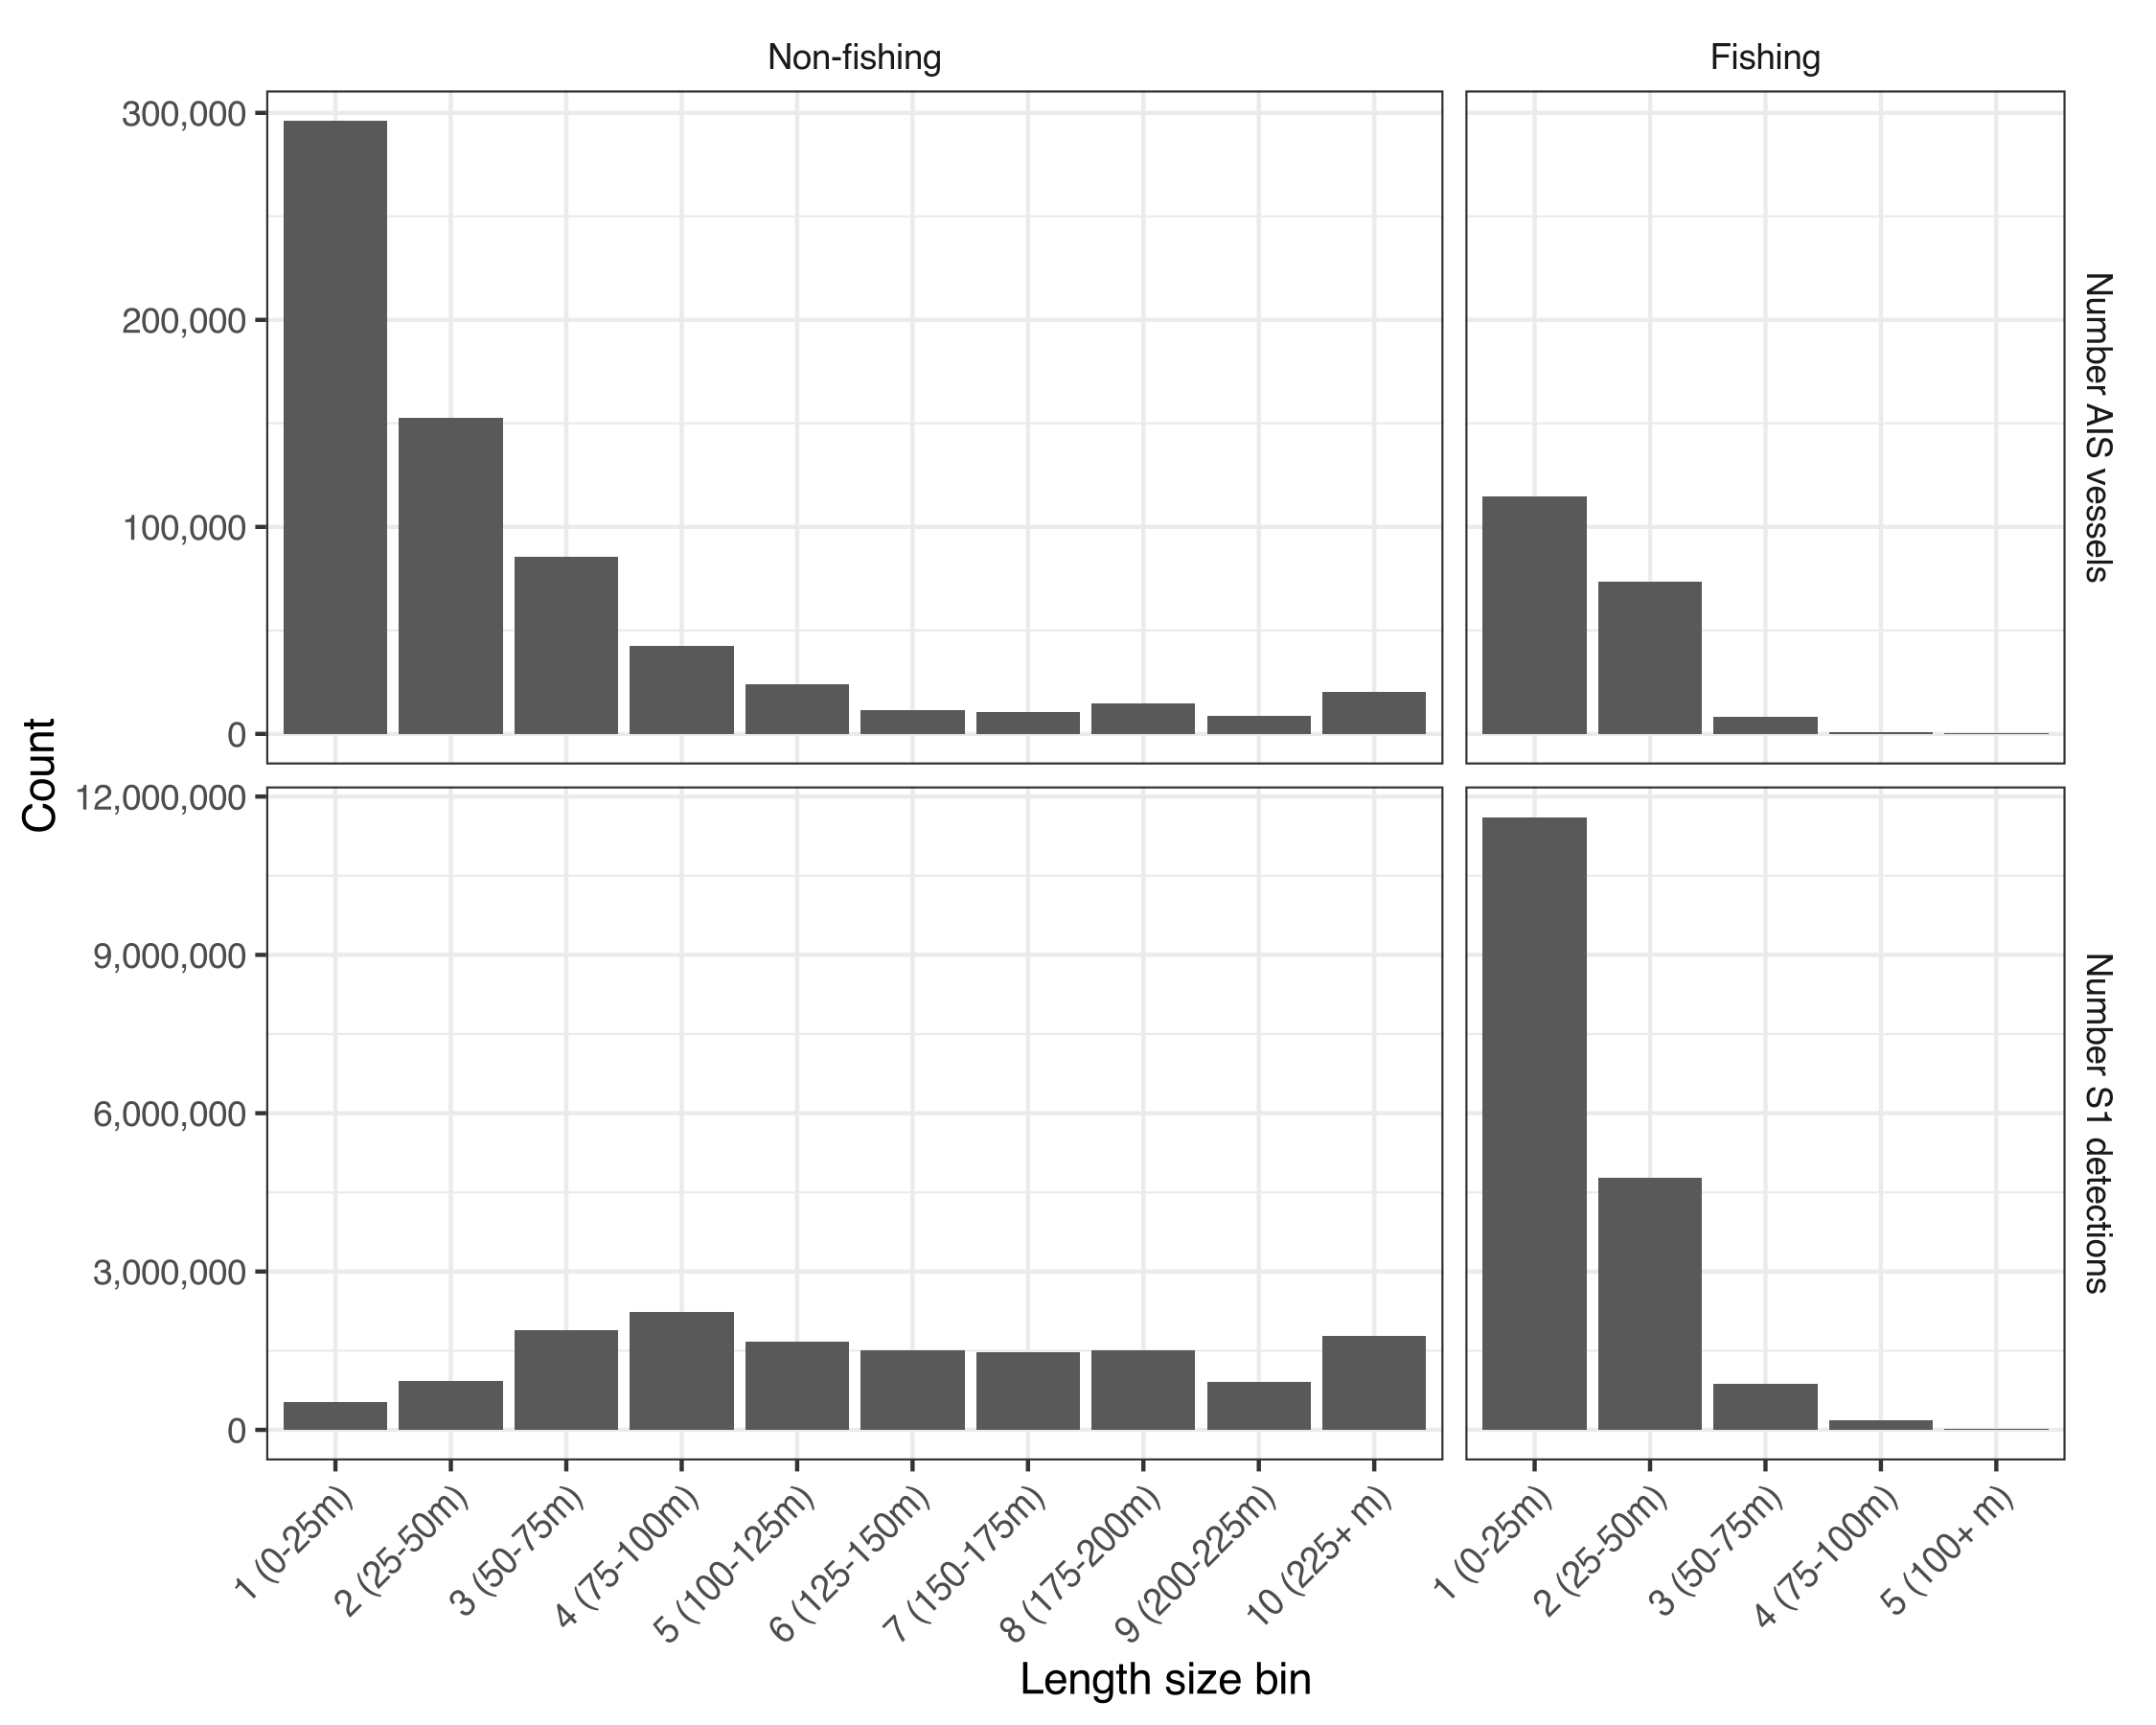
\includegraphics[width=\columnwidth]{figures/fig-length-bin-distributions-1.png}
    \caption{Distributions showing the number of unique AIS vessels and number of S1 detections for each length size bin, disaggregted by non-fishing and fishing vessels.}
    \label{fig:fig-length-bin-distributions}
\end{figure}

\begin{figure}[H]
    \centering
    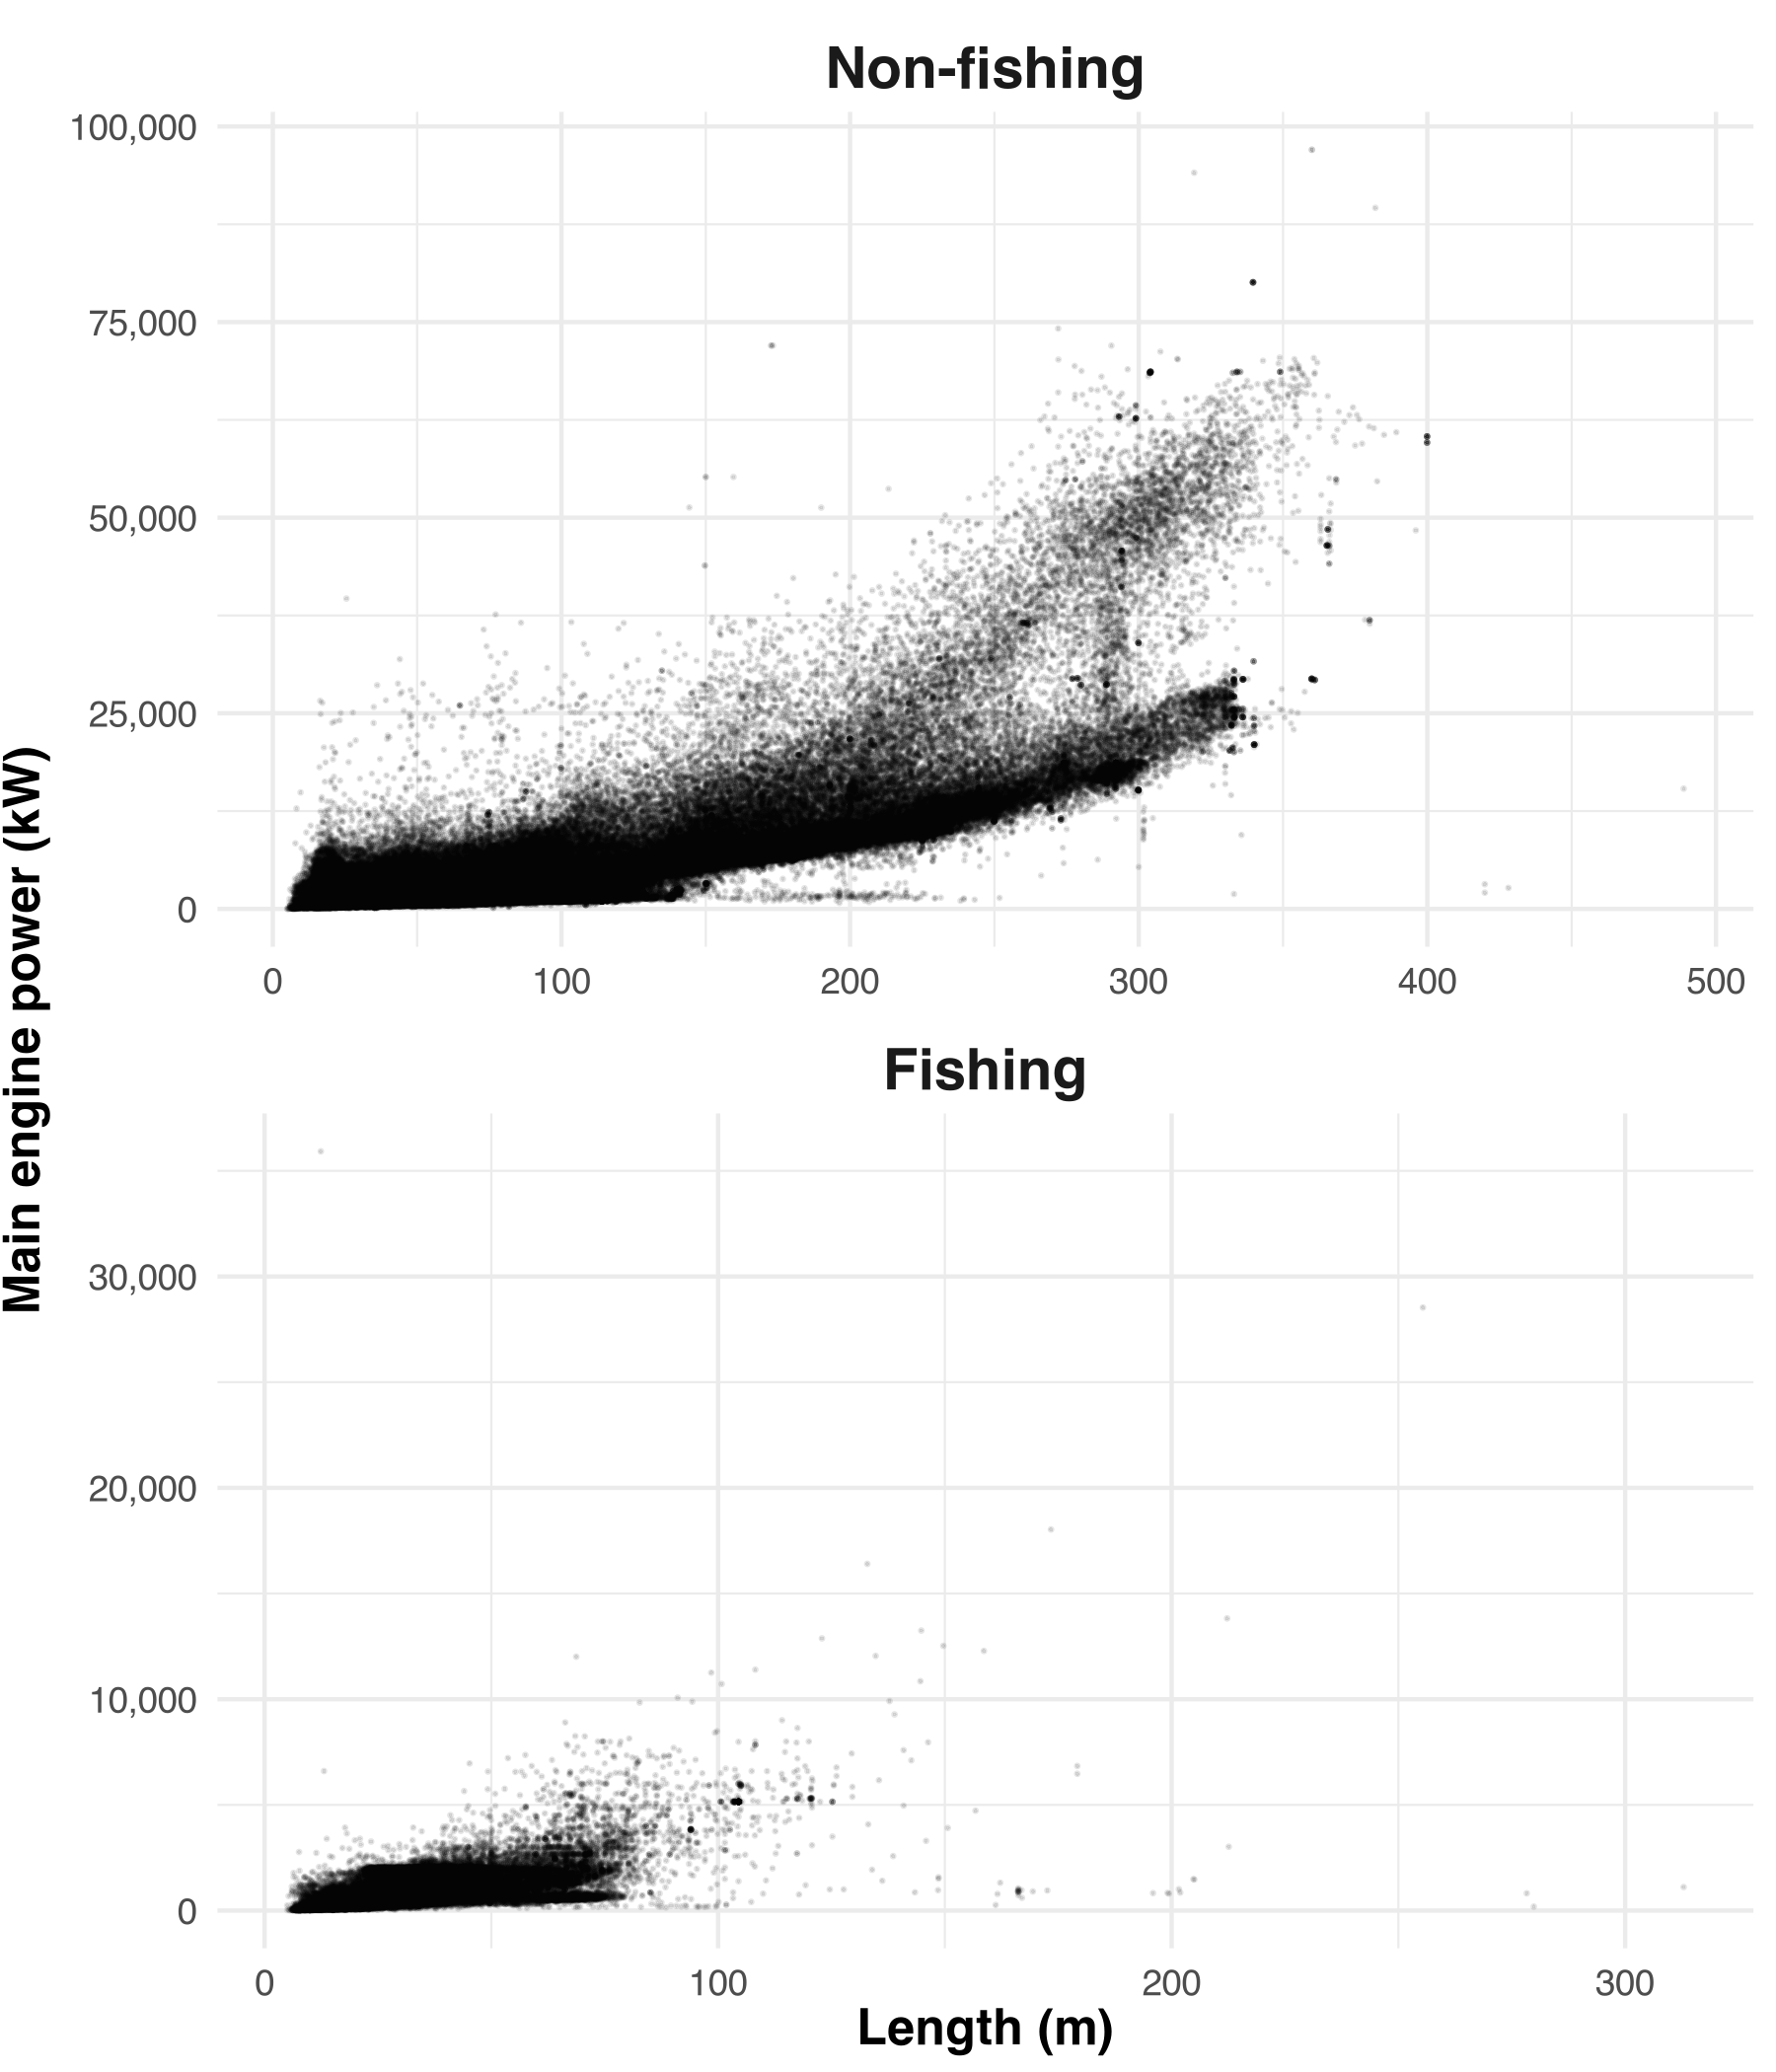
\includegraphics[width=\columnwidth]{figures/fig-ais-length-power-relationship-1.png}
    \caption{Relationship between main engine power (killowatts) and length (meters) for all AIS-broadcasting vessels, disaggregated by non-fishing and fishing vessels.}
    \label{fig:fig-ais-length-power-relationship}
\end{figure}

\paragraph{Detection classification}  Each observation unit is the boolean presence/absence of unmatched S1 detections in a given 1x1 degree ocean pixel, in a given month, for a given type of vessel (either non-fishing or fishing), for a given length bin.

\paragraph{Detection regression}  Each observation unit is the detection density of unmatched S1 detections in a given 1x1 degree ocean pixel, in a given month, for a given type of vessel (either non-fishing or fishing), for a given length bin. To calculate the detection density, we normalize detections by S1 sampling effort within each pixel and month, defined as the imaged area of each individual S1 scene overlapping that pixel, summed across scenes. Because a pixel that is imaged on several passes contributes its imaged area once per pass, this quantity is not simply the area imaged: it is equivalent to the area imaged at least once multiplied by the effective number of passes over it, and therefore carries units of km² × passes rather than km². Normalizing by it, rather than by area alone, is what makes detection counts comparable across pixels and months, because S1 detections are anonymous and recorded per pass: a vessel that never moves is detected twice in a pixel imaged twice, and only dividing by an effort measure that counts both passes recovers the same density in each case.

\subsubsection{Model features}

We define a global spatial resolution of 1x1-degree which is used for all spatial model features, and use a monthly temporal units for all temporal model features. All models features used across the three models are summarized in Table \ref{tab:data_sources} and described below.

\clearpage

\begin{table}[!h]
\centering
\caption{\label{tab:data_sources}Data sources for all included model features, including which random forest model uses the features (M1: detections classification; M2: detections regression; and/or M3: emissions regression), the units, feature type, whether it varies spatially, whether it varies temporally, and the source name and reference citation.}
\centering
\fontsize{4}{6}\selectfont
\begin{tabular}[t]{lllllllllll}
\toprule
Model feature & Category & M1 & M2 & M3 & Units & Type & Spatial & Temporal & Source & Ref.\\
\midrule
Presence/absence of unmatched S1 detections & Dependent variable & Yes & No & No & - & Boolean & Yes & Yes & GFW & \cite{paolo2024satellite}\\
Unmatched S1 detections per km2 imaged & Dependent variable & No & Yes & No & detects/km2 & Numeric & Yes & Yes & GFW & \cite{paolo2024satellite}\\
Log(AIS emissions) & Dependent variable & No & No & Yes & log(MT) & Numeric & Yes & Yes & GFW & -\\
Vessel type (fishing or non-fishing) & Dependent variable & Yes & Yes & Yes & - & Boolean & Yes & Yes & GFW & \cite{paolo2024satellite}\\
Lower threshold of vessel length bin & S1 detection features & Yes & Yes & No & m & Numeric & No & No & GFW & \cite{paolo2024satellite}\\
\addlinespace
Vessel length bin category & S1 detection features & Yes & Yes & No & - & Factor & Yes & Yes & GFW & \cite{paolo2024satellite}\\
S1 detections per km$^2$ of area for each length bin & S1 detection features & No & No & Yes & detects/km2 & Numeric & Yes & Yes & GFW & \cite{paolo2024satellite}\\
Total pixel area imaged by S1 across all time & S1 detection features & Yes & Yes & No & km2 & Numeric & Yes & No & GFW & \cite{paolo2024satellite}\\
Unique AIS-broadcasting vessels in pixel-month & AIS reception quality & Yes & Yes & No & - & Numeric & Yes & Yes & GFW & \cite{kroodsma2018tracking}\\
Unique AIS-broadcasting vessels globally & AIS reception quality & Yes & Yes & No & - & Numeric & No & Yes & GFW & \cite{kroodsma2018tracking}\\
\addlinespace
Positions reported by AIS type A & AIS reception quality & Yes & Yes & Yes & - & Numeric & Yes & No & GFW & \cite{kroodsma2018tracking}\\
Positions reported by AIS type B & AIS reception quality & Yes & Yes & Yes & - & Numeric & Yes & No & GFW & \cite{kroodsma2018tracking}\\
Proportion of messages, dynamic AIS receivers & AIS reception quality & Yes & Yes & Yes & - & Numeric & Yes & Yes & GFW & \cite{kroodsma2018tracking}\\
Proportion of messages, terrestrial AIS receivers & AIS reception quality & Yes & Yes & Yes & - & Numeric & Yes & Yes & GFW & \cite{kroodsma2018tracking}\\
Proportion of messages, satellite AIS receivers & AIS reception quality & Yes & Yes & Yes & - & Numeric & Yes & Yes & GFW & \cite{kroodsma2018tracking}\\
\addlinespace
Month of year & Temporal features & Yes & Yes & Yes & - & Factor & No & Yes & GFW & -\\
Post-2020 IMO Sulphur policy & Temporal features & No & No & Yes & - & Boolean & No & Yes & IMO & \cite{imo_sulphur_2020}\\
Ocean basin & Geographic features  & Yes & Yes & Yes & - & Factor & Yes & No & GFW & \cite{kroodsma2018tracking}\\
Pixel water area & Geographic features  & Yes & Yes & Yes & km2 & Numeric & Yes & No & GFW & \cite{paolo2024satellite}\\
Pixel water fraction & Geographic features & No & No & Yes & - & Numeric & Yes & No & GFW & \cite{paolo2024satellite}\\
\addlinespace
Mean ocean depth & Geographic features  & Yes & Yes & Yes & m & Numeric & Yes & No & GFW & \cite{kroodsma2018tracking}\\
Mean distance from shore & Geographic features  & Yes & Yes & Yes & m & Numeric & Yes & No & GFW & \cite{kroodsma2018tracking}\\
Mean distance from nearest port & Geographic features  & Yes & Yes & Yes & m & Numeric & Yes & No & GFW & \cite{kroodsma2018tracking}\\
Minimum distance to top 20 port & Geographic features  & Yes & Yes & Yes & m & Numeric & Yes & No & Lloyd’s List & \cite{LloydsListTopPorts2024}\\
Mean wind speed & Weather features & No & Yes & No & m/s & Numeric & Yes & Yes & ERA5 & \cite{era5cds2023}\\
\addlinespace
Mean significant wave and swell height & Weather features & No & Yes & No & m & Numeric & Yes & Yes & ERA5 & \cite{era5cds2023}\\
Mean wave period & Weather features & No & Yes & No & s & Numeric & Yes & Yes & ERA5 & \cite{era5cds2023}\\
Mean sea surface temperature & Weather features & No & Yes & No & K & Numeric & Yes & Yes & ERA5 & \cite{era5cds2023}\\
Mean sea level pressure & Weather features & No & Yes & No & Pa & Numeric & Yes & Yes & ERA5 & \cite{era5cds2023}\\
Total precipitation & Weather features & No & Yes & No & m & Numeric & Yes & Yes & ERA5 & \cite{era5cds2023}\\
\bottomrule
\end{tabular}
\end{table}

\FloatBarrier

\clearpage

\paragraph{S1 vessel detection features}

For the emissions regression model, we include several model features that capture the vessel length frequency distribution of S1 detections that occurred in any given pixel-month for each vessel type (fishing or non-fishing).This prevents assigning emissions to vessels for which no emission estimates are available. S1 detections smaller than the minimum vessel size represented in the AIS-broadcasting dataset are excluded to avoid assigning emissions to vessel sizes not characterized by the AIS emissions model. We normalize the detections by the same measure of S1 sampling effort described above — per-scene imaged area summed across all S1 scenes within each pixel-month, in km² × passes — to account for spatiotemporal variation in S1 sampling effort and therefore create a measure of detection density (Fig. \ref{fig:fig-map-fraction-months-imaged} shows spatial variation of sampling effort; Fig. \ref{fig:fig-s1-coverage-time-series} shows temporal variation). The emissions regression model is trained with these features corresponding to matched detection density in order to predict AIS-based emissions; when it comes time for using the model to predict S1-unmatched emissions, the unmatched detection density is used for these features instead.

For the detection classification and detection regression models, each unit of observation represents one of the vessel length bins for each pixel-month and vessel type. We also include two model features describing the length bin for each observation: the numeric lower threshold for the vessel length bin, and a categorical factor representing which of the length bins the observation belongs to. We finally include for each pixel the total S1 sampling effort accumulated across the entire 2017-2025 time period, again summed across scenes, in order to account for the general amount each pixel is imaged. 


\paragraph{Spatial features}

For each pixel we extract spatial information, including depth, distance to shore, and distance to the nearest port, from a high-resolution GFW subproduct (0.01x0.01-degree) and aggregate it to our 1x1-degree grid resolution by computing the minimum value in each pixel. In addition to the distance from the nearest port (which can be of any size port), we also include the distance from each pixel centroid to the nearest of the top 20 container ports according to the Lloyd's list of 2024 \cite{LloydsListTopPorts2024}. We include this since traffic density, loitering practices, and navigation behavior in major ports differ from those in regular ports. Additional geographic features include the total area covered by water within each pixel, the fraction of area within each pixel covered by water, and a categorical variable indicating which of the five major ocean basins each pixel falls within.

\paragraph{Weather features}

Weather influences both vessel activity as well as the ability for SAR to detect vessels. Storms or rough sea conditions may cause vessels, particularly smaller vessels, to stay in port during storms or avoid certain areas \cite{majamaki2025improving}. Sea surface temperature (SST) impacts the distribution of fish species, therefore impacting the spatiotemporal distribution of fishing vessels \cite{xing2026underestimated}. Weather and sea surface state also influences S1's ability to detect vessels. Sea surface waves generated by wind modify SAR background signal, directly affecting the ability of the S1 detection model to accurately identify vessels \cite{huo2018ship}. Heavy rain can also affect sea surface scatter and background cluttering \cite{greidanus2017sumo}, as can swell and wave height \cite{ryu2025environment}, affecting the ability of SAR to detect vessels. To account for these effects, we extracted weather data from ECMWF Reanalysis v5 (ERA5), the fifth-generation atmospheric reanalysis of the global climate, produced by the Copernicus Climate Change Service \cite{era5cds2023}. We used Google Earth Engine to extract hourly ERA5 data and aggregate it to monthly average or total values for the ocean area in each of our 1x1 degree pixels. As our final model features that were used in the detection regression model, we used mean wind speed (which may influence vessel activity and S1 detection), total precipitation (which may influence vessel activity), mean sea surface temperature (which may influence vessel activity, particularly for fishing vessels), mean sea level surface pressure (which may influence vessel activity), mean wave and swell height which may influence vessel activity), and mean wave period (which may influence vessel activity).

\paragraph{AIS reception quality features}

We included several model features related to AIS reception quality and signal type. To account for reception quality, we used two features: messages per day for AIS Type A and Type B transponders, capturing regional variation in AIS reception. Additionally, because AIS signals are received via different systems (terrestrial receivers, satellite receivers, and more recently dynamic receivers) we identified the associated receiver type for each ping and calculated the proportion of each type per pixel and month, summing to one. These features describing AIS coverage and the predominance of receiver types influence the fraction of broadcasting versus non-broadcasting vessels, and thus the associated emissions and detections.

\paragraph{Temporal features}

To account for temporal variability in each of the three models, we include a factor feature representing the month of the year. We also include a boolean feature for whether or not the observation occurs on or after January 2020, to coincide with the start of the IMO low sulfur fuel policy. To account for temporal trends of general vessel activity in the detection classification and regression models, we include features characterizing the total number of unique AIS-broadcasting vessels globally each month, as well as the number of unique AIS-broadcasting vessels in each pixel-month. Accounting for temporal variation is particularly important given both the variation in S1 coverage over time, as well as the variation in global fleet composition over time (Fig. \ref{fig:fig-s1-coverage-time-series}).

\subsubsection{Data pre-processing}

We perform the following data pre-processing steps, in this order, each time a model is trained or predictions are inferred. In order to avoid data leakage during performance testing, data pre-processing that performs calculations that directly use the data (i.e., imputation of missing values) is always performed  on the training data. To do so, we leverage the recipes package in R \cite{recipes}.

1. We treat several features as categorical (fishing or non-fishing; the post-2020 temporal boolean; ocean; and for the detection classification and regression models that are disaggregated by vessel length bin, we treat the length bin as categorical)

2. For any missing values of numeric model features, we impute their value using the median of that feature's non-missing values.

3. We remove any numeric model features that are highly correlated with other features (i.e., that have a Pearson's correlation coefficient of $>$ 0.9).

\subsubsection{Model training}

We defined three independent Random Forest models using the tidymodels framework in R \cite{tidymodels}. Model fitting was done using the ranger engine \cite{ranger} in parsnip \cite{parsnip}. We  use 500 trees for each forest, and otherwise use default hyperparameter settings for ranger. We perform several out-of-sample performance tests for each model using independent training and testing data splits to assess how well it does for predictions inside the S1 footprint, as well as a simulation of how well it would do for predictions outside the footprint. We train each of the three final models using the entire dataset.

For the detection presence/absence classification model, we use an additional validation dataset to optimize the classification cutoff threshold to maximize the F1 score (the harmonic mean of precision and recall). So for performance tests, we train the model on a training dataset, calibrate the classification threshold on the validation dataset, and then test performance on the testing dataset using the optimized threshold. For the final model, we train the model using a training dataset, calibrate the classification threshold on a validation dataset, and then train a final model using the entire dataset and the optimized threshold.

For the eight linear regression models to convert CO$_2$ emissions to emissions of other GHGs and pollutants, we use the lm function from the base R stats package \cite{r}.

\subsubsection{Model testing}

We assessed model performance for each of the three models using two different evaluation approaches designed to test: 1) predictive power for areas within the S1 footprint but that don't have overpasses in a given month (subsequently referred to as our 'inside footprint' test); and 2) the models' ability to generalize to locations completely outside the S1 footprint (subsequently referred to as our 'simulated outside footprint' test).

\paragraph{Inside S1 footprint testing}

Because both emissions and detection predictions inside the S1 footprint are made for locations where emissions and detections data is available for training, (i.e., inside the footprint we are not generalizing to regions with unknown emissions and detections), we first evaluated performance inside the footprint using a stratified random $80\%$/$20\%$ training/testing split. For each of the three models, we stratify the random split by the dependent variable (presence/absence of unmatched detections for the detections classification model; density of unmatched detections for the detections regression model; and log-transformed emissions for the emissions regression model). 

For the detection presence/absence classification model, we use an additional validation dataset to optimize the classification cutoff threshold. In this case, we use a $60\%$/$20\%$/$20\%$ training/ validation/ testing split.

\paragraph{Simulated outside S1 footprint testing}

Then, to assess spatial transferability when predicting emissions in areas completely outside the S1 footprint (i.e., areas far from shore), we implement a spatially structured split, training on nearshore pixels ($<=$ 100km from the nearest port) and testing on offshore pixels ($>$ 100km from the nearest port) (Fig. \ref{fig:fig-offshore-outside-footprint-training-testing-map}). 

For the detection presence/absence classification model, we again use an additional validation dataset to optimize the classification cutoff threshold. We therefore use data from nearshore pixels to create a stratified random $80\%$/$20\%$ training/validation split, and then test using the offshore pixels.


\begin{figure}[H]
    \centering    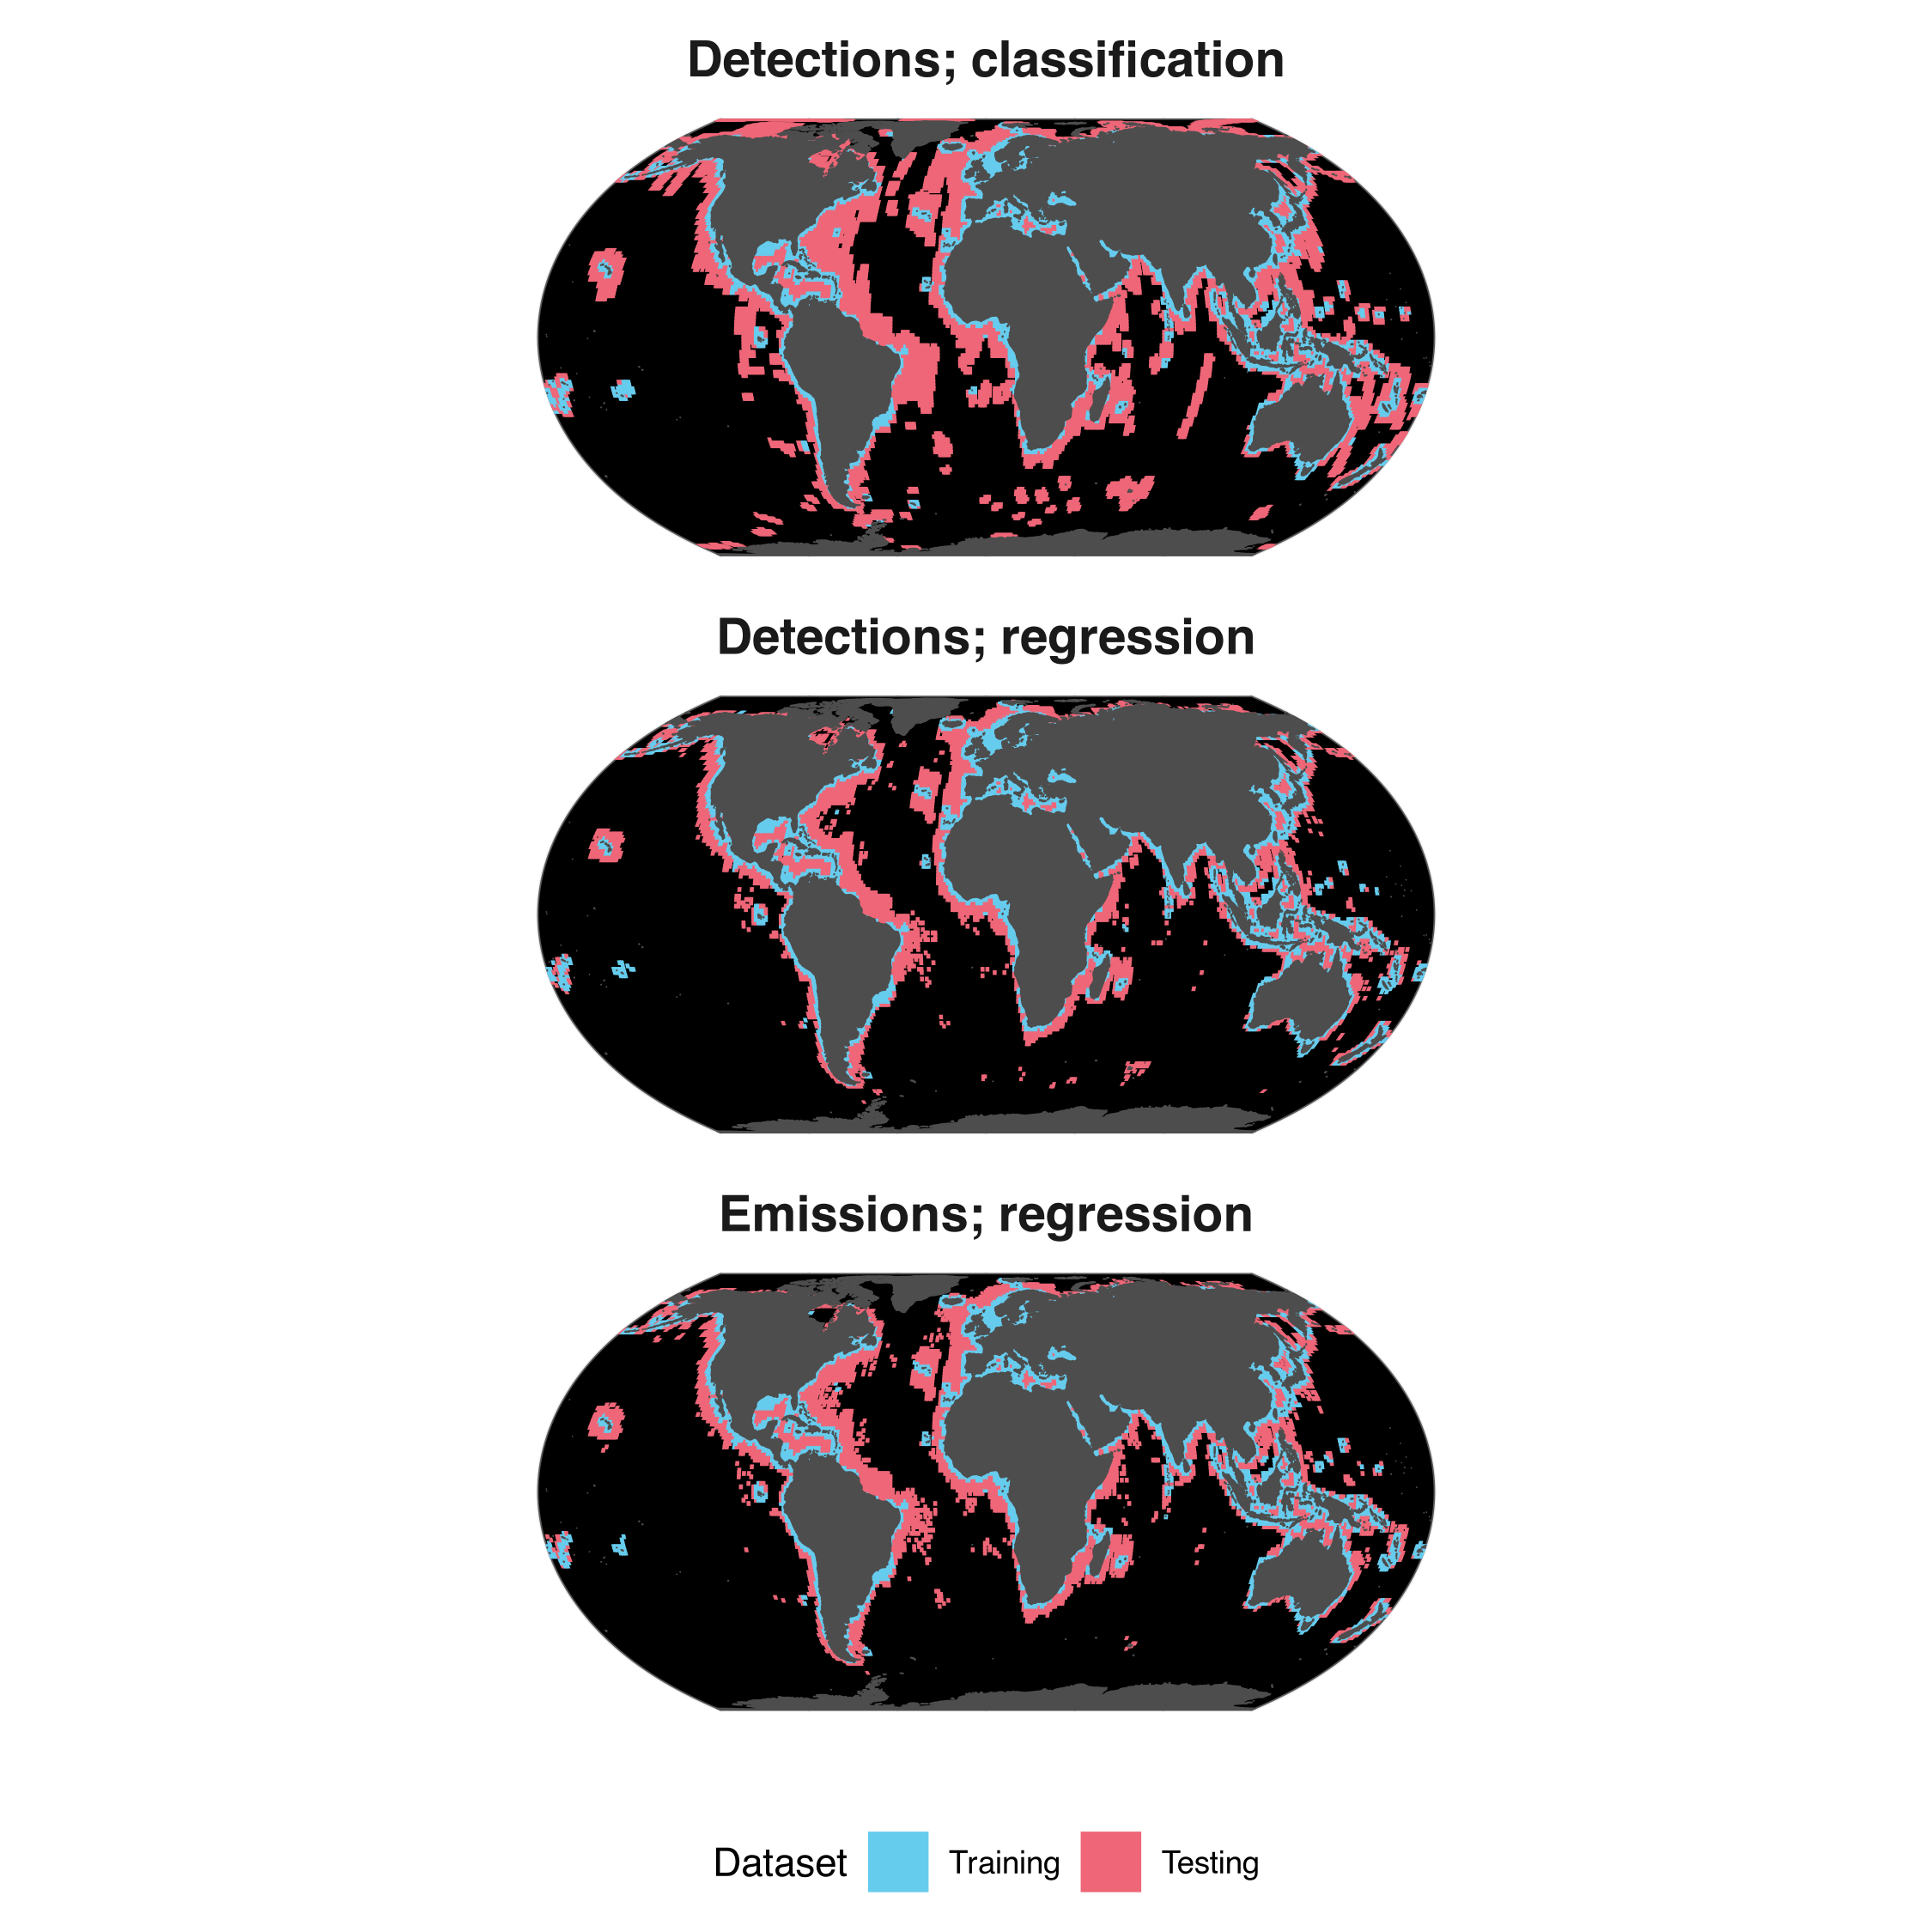
\includegraphics[width=\columnwidth]{figures/fig-offshore-outside-footprint-training-testing-map-1.png}
    \caption{Maps of pixels that were used in the training and testing datasets for the simulated outside S1 footprint performance tests for each model. Pixels $<=$ 100km from the shore were used for training; pixels $>$ 100km from shore were used for testing.}
    \label{fig:fig-offshore-outside-footprint-training-testing-map}
\end{figure}

Classifier performance is reported using precision-recall curves (Fig. \ref{fig:fig-pr-curves}), receiver operating characteristic (ROC) curves (Fig. \ref{fig:fig-roc-curves}), and confusion matrices (Fig. \ref{fig:fig-conf-mat}). Table \ref{tab:all_performance_metrics_table} also summarizes regression performance for detections, both inside and outside the footprint, alongside the emissions model performance. To assess the performance of the emissions model, predicted log emissions were back-transformed using Duan’s smearing coefficient, calculated from the residuals of the training data \cite{duan1983smearing}. The same transformation was applied to the final model prediction.

For the CO$_2$ emissions regression random forest, we simply train the model on the training data and test the model on the testing data (using the two sets of splits described above for inside and outside the S1 footprint tests). For the other eight gases, we: 1) train the linear regression using the training data (to convert CO$_2$ emissions to emissions of each gas); 2) use the CO$_2$ emissions regression random forest to predict emissions for the testing data; and then 3) use the predicted CO$_2$ emissions for the testing data and then convert this to emissions for each of the other eight gases using the eight linear regressions built in step 2; and then 4) compare the predicted emissions of each of the eight gases against the observed emissions of each of the eight gases in the training data. In this way, we are able to measure fully out-of-sample performance for predicting not only CO$_2$, but also all of the other two GHGs and six pollutants.


\begin{figure}[H]
    \centering
    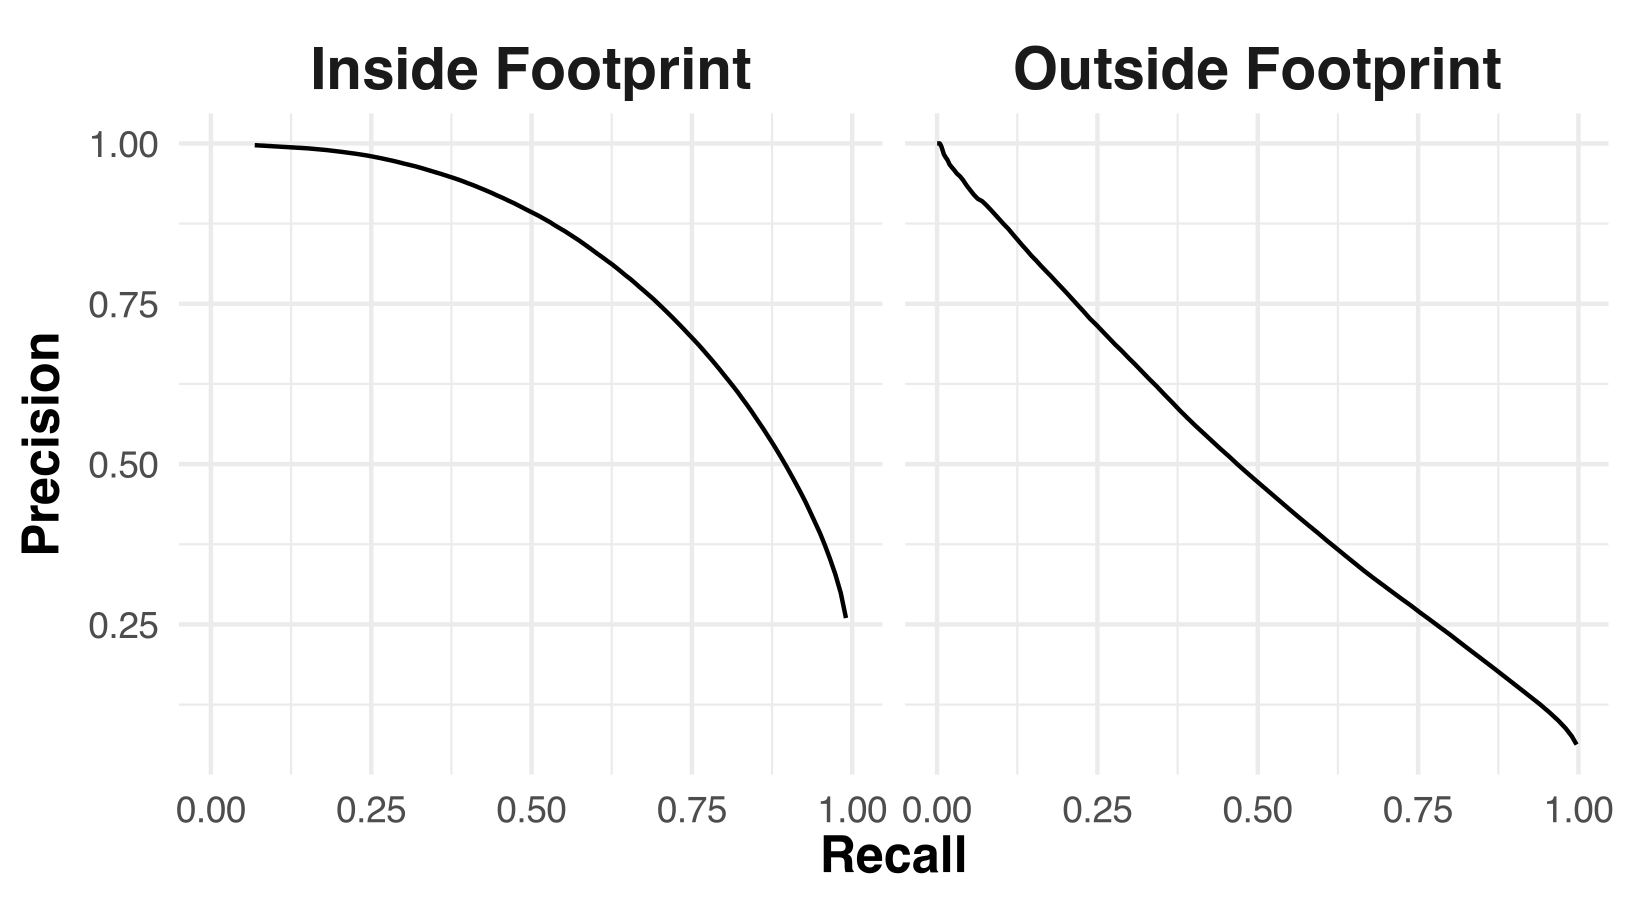
\includegraphics[width=\columnwidth]{figures/fig-pr-curves-1.png}
    \caption{Precision-recall curves of the detection presence/absence classification model, shown for both the inside S1 footprint test and simulated outside S1 footprint test.}
    \label{fig:fig-pr-curves}
\end{figure}

\begin{figure}[H]
    \centering
    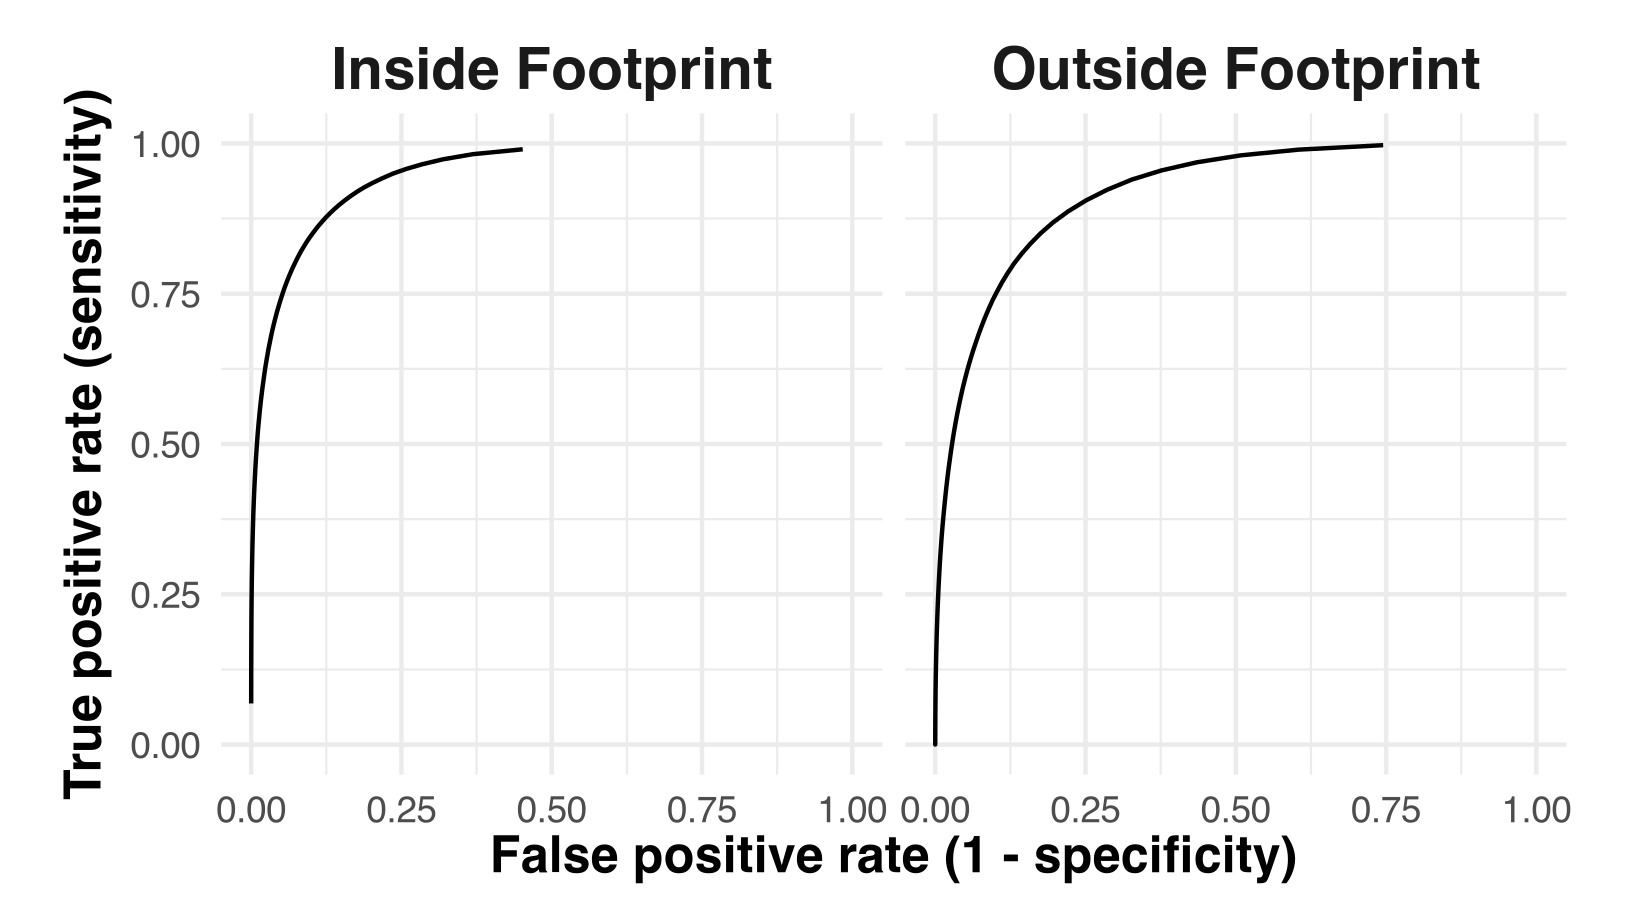
\includegraphics[width=\columnwidth]{figures/fig-roc-curves-1.png}
    \caption{Receiver Operating Characteristic (ROC) curves of the detection classification model, shown for both the inside S1 footprint test and simulated outside S1 footprint test.}
    \label{fig:fig-roc-curves}
\end{figure}

\begin{figure}[H]
    \centering
    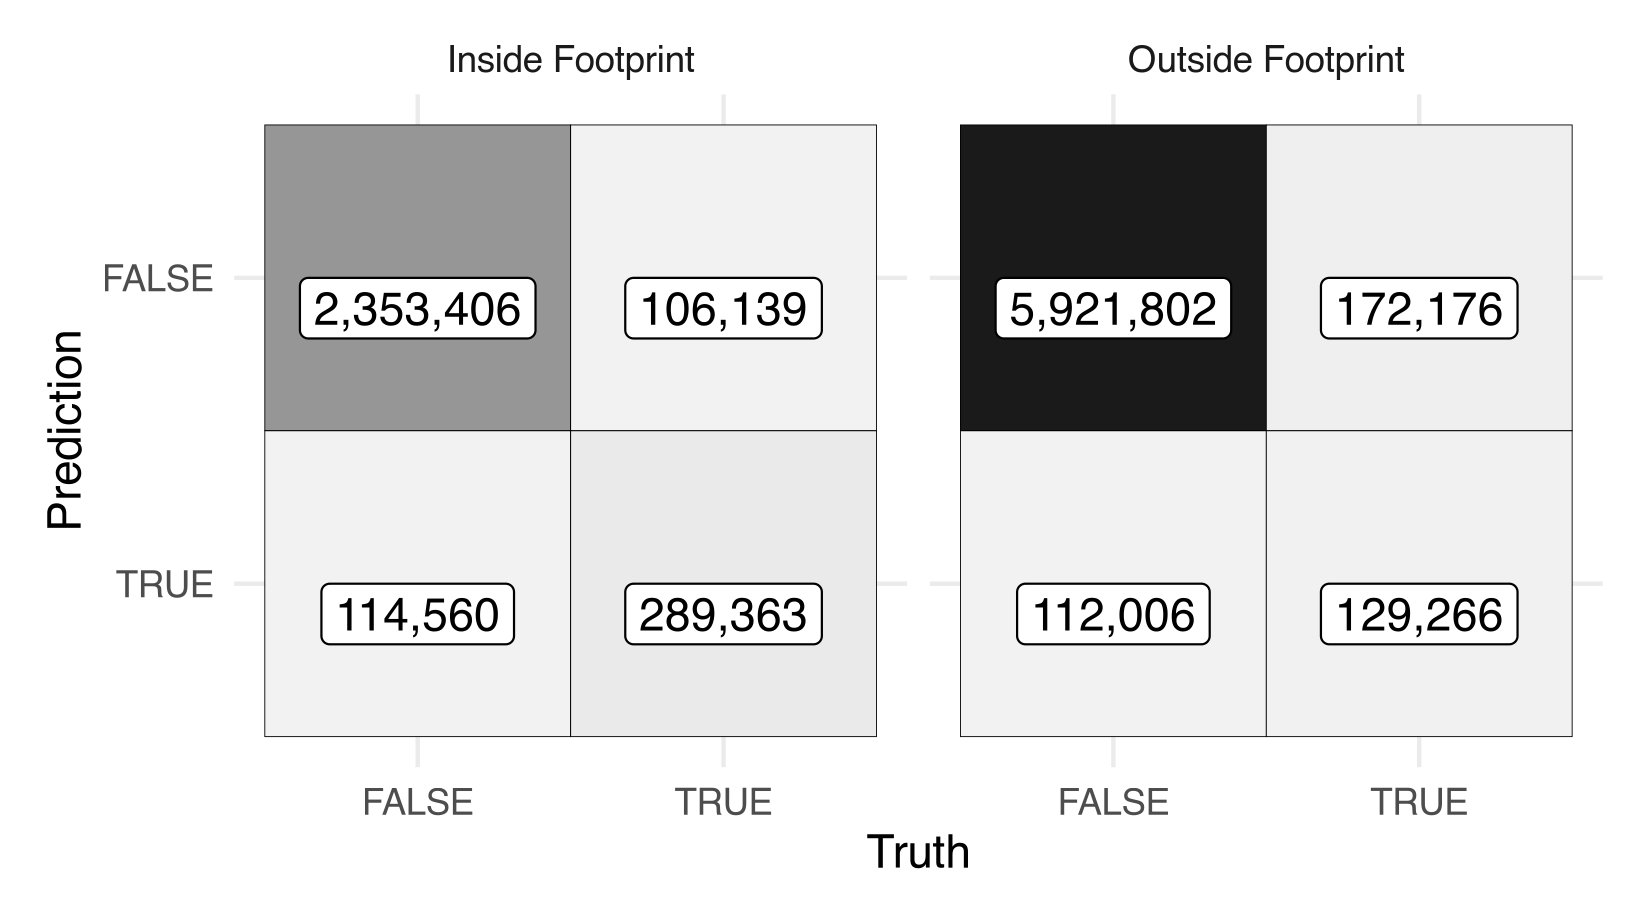
\includegraphics[width=\columnwidth]{figures/fig-conf-mat-1.png}
    \caption{Confusion matrices of the detection classification model, shown for both the inside S1 footprint test and simulated outside S1 footprint test.}
    \label{fig:fig-conf-mat}
\end{figure}


\begin{table}[!h]
\centering
\caption{\label{tab:all_performance_metrics_table}Summary of dark fleet model performance metrics for the: 1) emissions regression model; 2) detections classification mode; and 3) detections regression model. Performance estimates for each metric are shown for both the inside S1 footprint and outside S1 footprint tests. All metrics are calculated at the unit of observation except for 'Total percent error', which is the percentage error in the total sum of all predictions relative to the total sum of all truth values.}
\centering
\fontsize{7}{9}\selectfont
\begin{tabular}[t]{l|l|l|r|r}
\hline
Model & Pollutant & Metric & Inside footprint & Outside footprint\\
\hline
Emissions regression & CO2 & Traditional R² & 0.94 & 0.74\\
\hline
Emissions regression & CH4 & Traditional R² & 0.91 & 0.64\\
\hline
Emissions regression & N2O & Traditional R² & 0.95 & 0.72\\
\hline
Emissions regression & CO & Traditional R² & 0.92 & 0.64\\
\hline
Emissions regression & NOX & Traditional R² & 0.87 & 0.59\\
\hline
Emissions regression & SOX & Traditional R² & 0.96 & 0.74\\
\hline
Emissions regression & PM2.5 & Traditional R² & 0.94 & 0.66\\
\hline
Emissions regression & PM10 & Traditional R² & 0.94 & 0.66\\
\hline
Emissions regression & VOCs & Traditional R² & 0.88 & 0.61\\
\hline
Emissions regression & CO2 & Total percent error & -7.76 & -9.97\\
\hline
Emissions regression & CH4 & Total percent error & -19.21 & -29.90\\
\hline
Emissions regression & N2O & Total percent error & -9.82 & -15.41\\
\hline
Emissions regression & CO & Total percent error & -18.06 & -29.18\\
\hline
Emissions regression & NOX & Total percent error & -22.54 & -36.33\\
\hline
Emissions regression & SOX & Total percent error & -5.51 & -8.02\\
\hline
Emissions regression & PM2.5 & Total percent error & -14.53 & -25.16\\
\hline
Emissions regression & PM10 & Total percent error & -14.53 & -25.16\\
\hline
Emissions regression & VOCs & Total percent error & -21.12 & -32.35\\
\hline
Detections classification & - & Accuracy & 0.92 & 0.96\\
\hline
Detections classification & - & F1 score & 0.72 & 0.48\\
\hline
Detections classification & - & Precision & 0.72 & 0.54\\
\hline
Detections classification & - & Precision-recall AUC & 0.81 & 0.50\\
\hline
Detections classification & - & Recall & 0.73 & 0.43\\
\hline
Detections classification & - & ROC AUC & 0.95 & 0.92\\
\hline
Detections classification & - & Sensitivity & 0.73 & 0.43\\
\hline
Detections classification & - & Specificity & 0.95 & 0.98\\
\hline
Detections regression & - & Traditional R² & 0.69 & 0.36\\
\hline
Detections regression & - & Total percent error & 1.09 & 20.46\\
\hline
\end{tabular}
\end{table}

\FloatBarrier

\subsubsection{Feature importance}

After assessing model performance, we perform a final fit using the entire dataset to assess feature importance for the three S1-unmatched emissions random forest models (Fig \ref{fig:fig-feature-importance}). Feature importance was quantified using the bias-corrected Gini index \cite{nembrini2018revival}, as implemented for random forests in the ranger R package \cite{ranger}. This metric quantifies how much each model feature reduces node impurity when it is used to make splits in the random forest's decision trees.

\begin{figure}[!p]
    \centering
    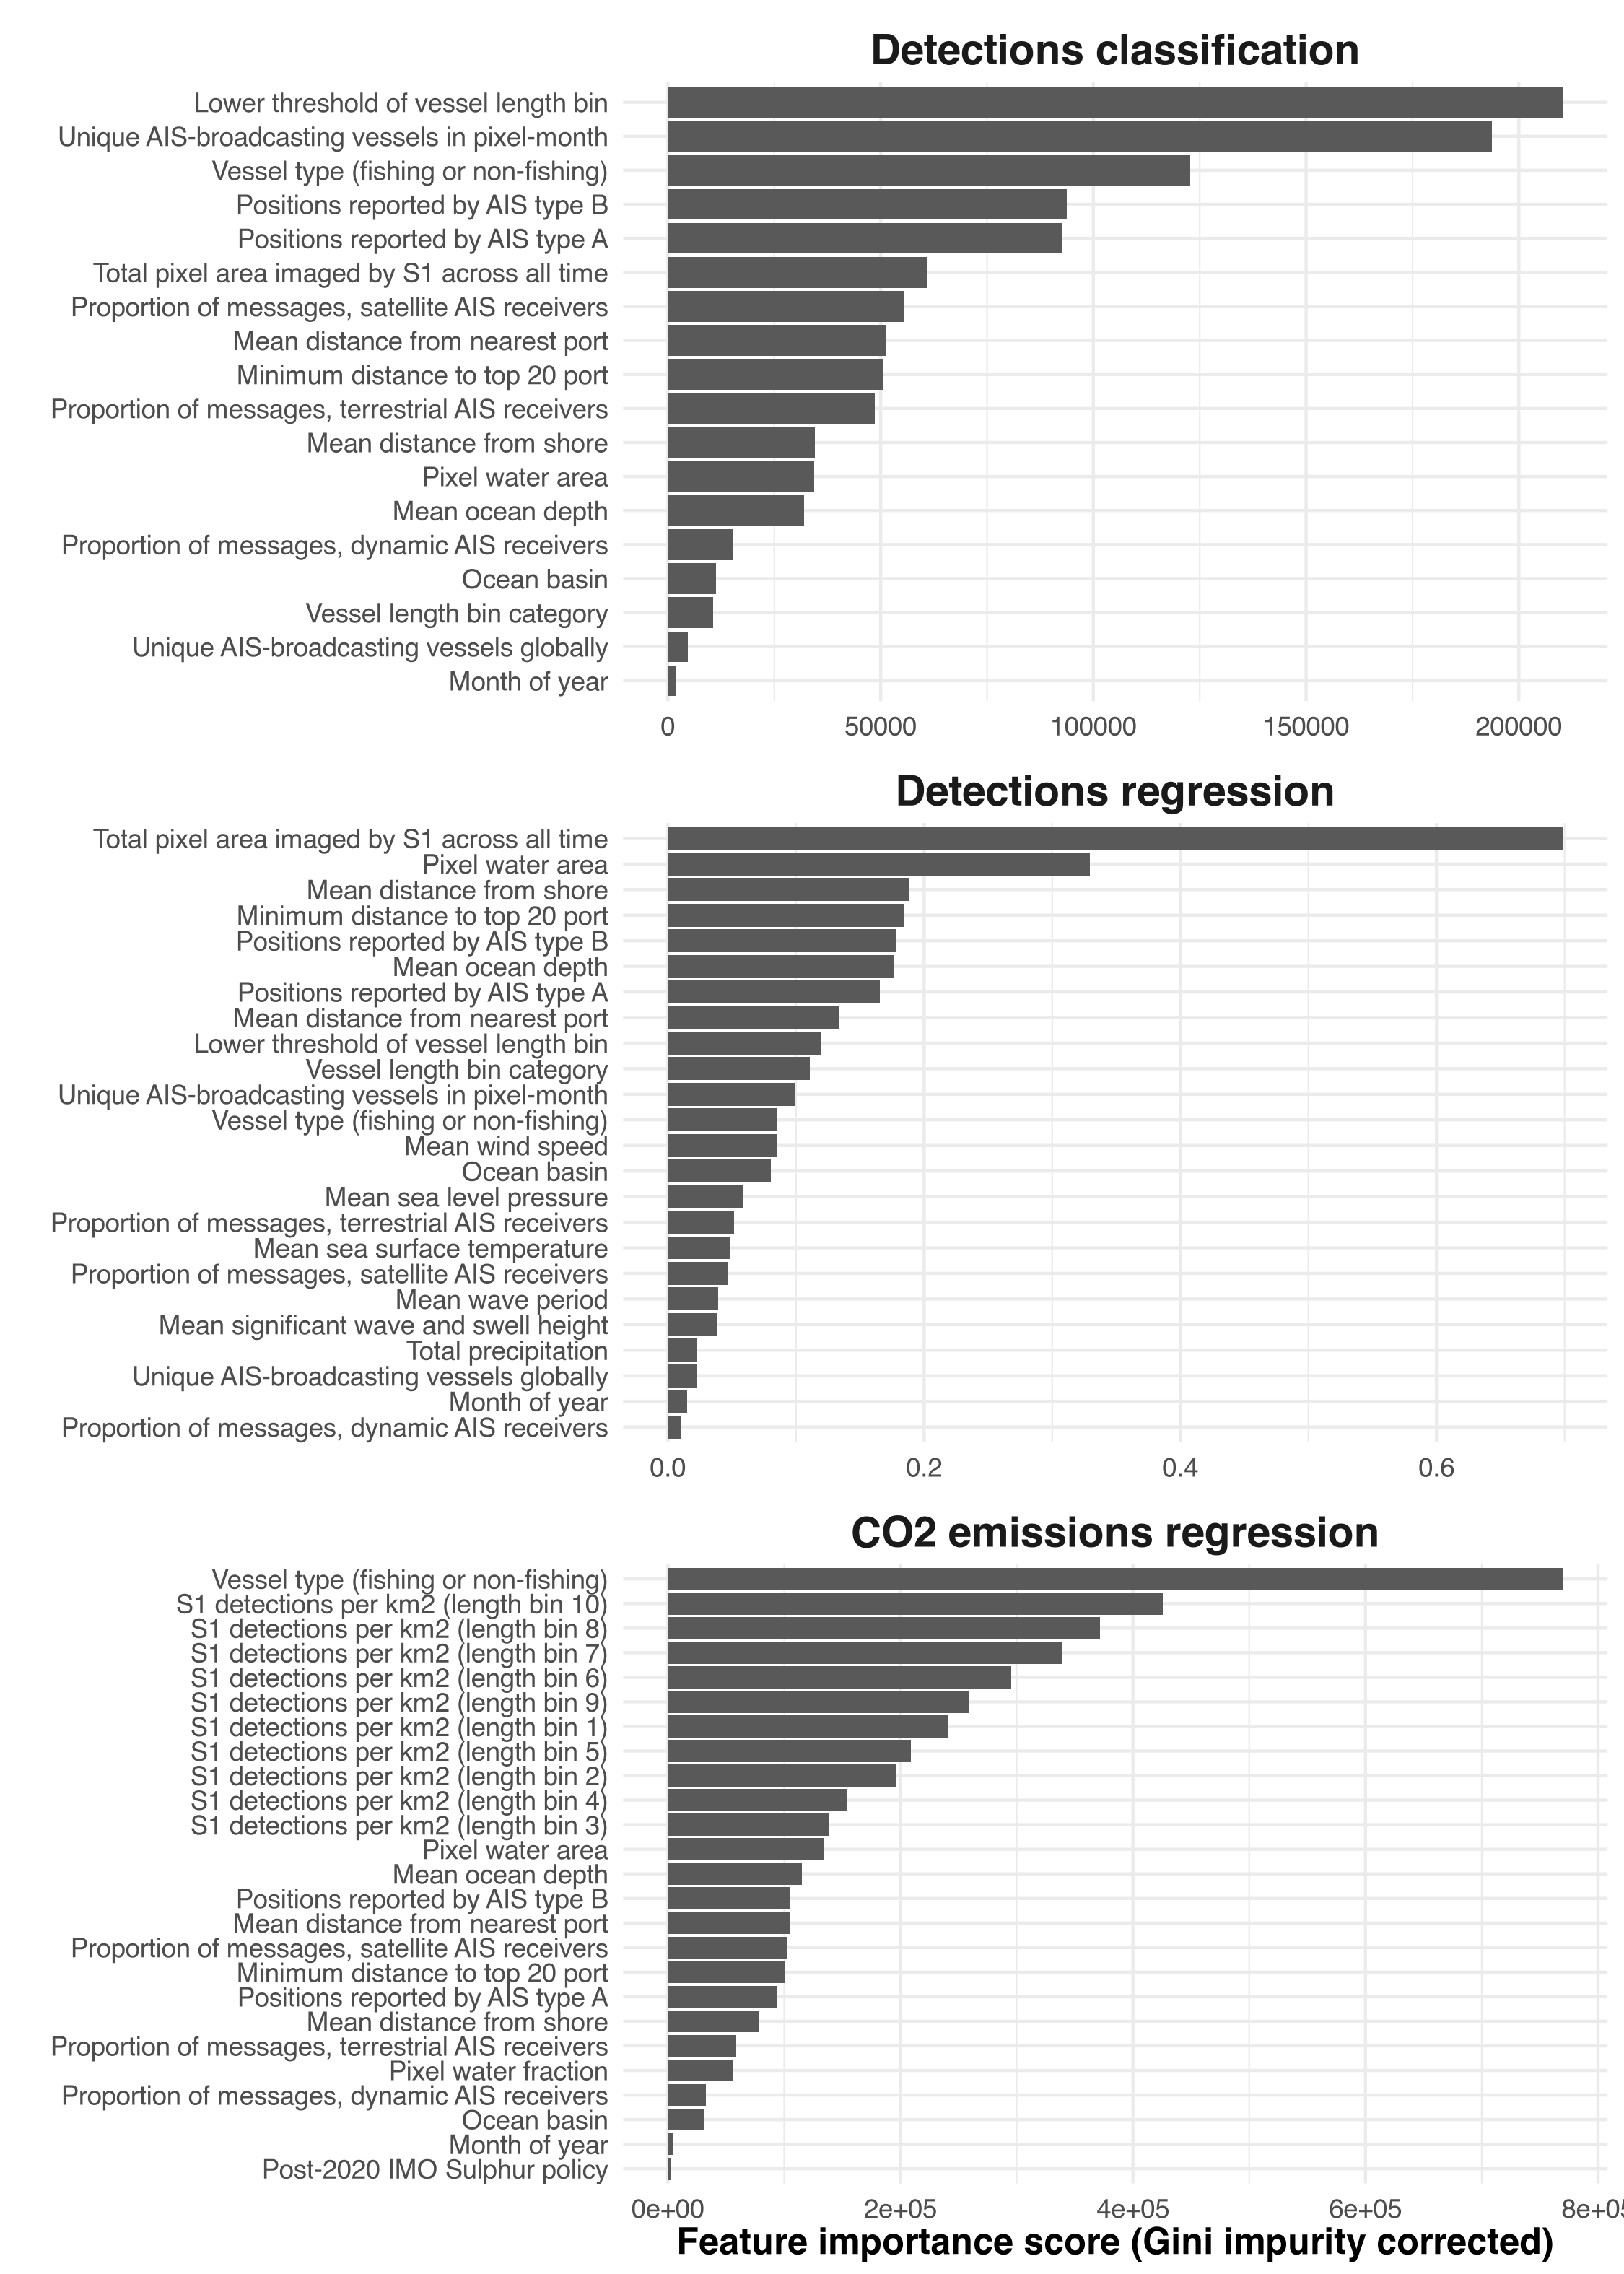
\includegraphics[width=\columnwidth]{figures/fig-feature-importance-1.png}
    \caption{Feature importance plots for the: 1) detections (presence/absence) classification model;
2) detections regression model; and 3) CO$_2$ emissions regression model.}
    \label{fig:fig-feature-importance}
\end{figure}

\subsubsection{Linear regression fit statistics for non-gas models}

Here we look at the linear regression fit statistics for the final models to convert CO$_2$ emissions to emissions of non-CO$_2$ gases (other GHGs and non-GHG pollutants), trained using the full dataset (Table \ref{tab:lm_other_gases_tidy_fit_stats}).

\begin{table}[!h]
\centering
\caption{\label{tab:lm_other_gases_tidy_fit_stats}Linear regression fit statistics for the final models trained to estimate emissions of non-CO$_2$ gases from CO$_2$ emissions. The model for each gas is a zero-intercept linear regression with 5 terms: CO$_2$ emissions interacted with each combination of period (pre/post-2020 IMO sulphur policy) and vessel type (fishing/non-fishing), plus CO$_2$ emissions interacted with the log of mean distance from shore.}
\centering
\fontsize{7}{9}\selectfont
\begin{tabular}[t]{l|l|l|l|r|l}
\hline
Pollutant & Term & Estimate & SE & T-stat. & p-value\\
\hline
CH4 & CO2 : log(distance from shore + 1) & 1.25e-06 & 3.29e-09 & 380.0 & $<$0.001\\
\hline
CH4 & CO2 : pre-2020 : non-fishing & -1.21e-06 & 3.17e-08 & -38.1 & $<$0.001\\
\hline
CH4 & CO2 : pre-2020 : fishing & 3.69e-06 & 8.41e-08 & 43.9 & $<$0.001\\
\hline
CH4 & CO2 : post-2020 : non-fishing & -1.92e-06 & 3.14e-08 & -61.4 & $<$0.001\\
\hline
CH4 & CO2 : post-2020 : fishing & 3.73e-06 & 4.52e-08 & 82.7 & $<$0.001\\
\hline
N2O & CO2 : log(distance from shore + 1) & 7.13e-07 & 2.32e-09 & 308.1 & $<$0.001\\
\hline
N2O & CO2 : pre-2020 : non-fishing & 4.17e-05 & 2.23e-08 & 1870.0 & $<$0.001\\
\hline
N2O & CO2 : pre-2020 : fishing & 4.30e-05 & 5.92e-08 & 727.2 & $<$0.001\\
\hline
N2O & CO2 : post-2020 : non-fishing & 4.12e-05 & 2.20e-08 & 1866.4 & $<$0.001\\
\hline
N2O & CO2 : post-2020 : fishing & 4.39e-05 & 3.18e-08 & 1380.3 & $<$0.001\\
\hline
CO & CO2 : log(distance from shore + 1) & 6.02e-05 & 1.57e-07 & 382.4 & $<$0.001\\
\hline
CO & CO2 : pre-2020 : non-fishing & 2.91e-05 & 1.51e-06 & 19.2 & $<$0.001\\
\hline
CO & CO2 : pre-2020 : fishing & 2.73e-04 & 4.02e-06 & 67.9 & $<$0.001\\
\hline
CO & CO2 : post-2020 : non-fishing & -5.48e-06 & 1.50e-06 & -3.7 & $<$0.001\\
\hline
CO & CO2 : post-2020 : fishing & 2.76e-04 & 2.16e-06 & 128.1 & $<$0.001\\
\hline
NOX & CO2 : log(distance from shore + 1) & 2.02e-03 & 4.33e-06 & 466.8 & $<$0.001\\
\hline
NOX & CO2 : pre-2020 : non-fishing & -7.34e-03 & 4.16e-05 & -176.3 & $<$0.001\\
\hline
NOX & CO2 : pre-2020 : fishing & -9.75e-04 & 1.10e-04 & -8.8 & $<$0.001\\
\hline
NOX & CO2 : post-2020 : non-fishing & -8.45e-03 & 4.12e-05 & -205.3 & $<$0.001\\
\hline
NOX & CO2 : post-2020 : fishing & -2.14e-03 & 5.93e-05 & -36.1 & $<$0.001\\
\hline
SOX & CO2 : log(distance from shore + 1) & -1.24e-05 & 7.15e-08 & -173.1 & $<$0.001\\
\hline
SOX & CO2 : pre-2020 : non-fishing & 6.30e-03 & 6.88e-07 & 9167.7 & $<$0.001\\
\hline
SOX & CO2 : pre-2020 : fishing & 6.37e-03 & 1.83e-06 & 3487.2 & $<$0.001\\
\hline
SOX & CO2 : post-2020 : non-fishing & 1.66e-03 & 6.81e-07 & 2442.1 & $<$0.001\\
\hline
SOX & CO2 : post-2020 : fishing & 1.67e-03 & 9.81e-07 & 1706.2 & $<$0.001\\
\hline
PM2.5 & CO2 : log(distance from shore + 1) & 3.65e-05 & 9.11e-08 & 401.1 & $<$0.001\\
\hline
PM2.5 & CO2 : pre-2020 : non-fishing & 4.14e-04 & 8.76e-07 & 472.7 & $<$0.001\\
\hline
PM2.5 & CO2 : pre-2020 : fishing & 5.33e-04 & 2.33e-06 & 229.0 & $<$0.001\\
\hline
PM2.5 & CO2 : post-2020 : non-fishing & 5.04e-05 & 8.67e-07 & 58.2 & $<$0.001\\
\hline
PM2.5 & CO2 : post-2020 : fishing & 2.10e-04 & 1.25e-06 & 168.4 & $<$0.001\\
\hline
PM10 & CO2 : log(distance from shore + 1) & 3.97e-05 & 9.90e-08 & 401.1 & $<$0.001\\
\hline
PM10 & CO2 : pre-2020 : non-fishing & 4.50e-04 & 9.52e-07 & 472.7 & $<$0.001\\
\hline
PM10 & CO2 : pre-2020 : fishing & 5.79e-04 & 2.53e-06 & 229.0 & $<$0.001\\
\hline
PM10 & CO2 : post-2020 : non-fishing & 5.48e-05 & 9.42e-07 & 58.2 & $<$0.001\\
\hline
PM10 & CO2 : post-2020 : fishing & 2.29e-04 & 1.36e-06 & 168.4 & $<$0.001\\
\hline
VOCs & CO2 : log(distance from shore + 1) & 1.00e-04 & 2.02e-07 & 495.8 & $<$0.001\\
\hline
VOCs & CO2 : pre-2020 : non-fishing & -3.94e-04 & 1.94e-06 & -203.1 & $<$0.001\\
\hline
VOCs & CO2 : pre-2020 : fishing & -2.01e-04 & 5.15e-06 & -39.1 & $<$0.001\\
\hline
VOCs & CO2 : post-2020 : non-fishing & -4.38e-04 & 1.92e-06 & -228.1 & $<$0.001\\
\hline
VOCs & CO2 : post-2020 : fishing & -2.10e-04 & 2.77e-06 & -75.7 & $<$0.001\\
\hline
\end{tabular}
\end{table}

\FloatBarrier

\subsubsection{Predicting S1-unmatched emissions}

To generate the final global estimates of S1-unmatched emissions, we: 1) train all models (the three random forests and eight linear regressions) using the entire dataset of observations that have both S1 detections and AIS emissions (Fig \ref{fig:fig-feature-importance}, Table \ref{tab:lm_other_gases_tidy_fit_stats}; noting that again for the presence/absence detection classification model, we use a random stratified training/validation split to first calibrate the classification threshold before fitting the final model on all the data); 2) then applied the final trained models across all ocean pixels on a monthly basis for the entire 2017-2025 study period. The prediction workflow followed a hierarchical logic based on the availability of S1 detections:

1. Direct estimation: If unmatched S1 detections are available for a given pixel-month, we use the unmatched detection density to directly predict S1-unmatched CO$_2$ emissions using the emissions regression model. We then use the other eight gas-specific linear regression models to convert CO$_2$ emissions to emissions of each of the other eight gases.
2. Indirect estimation: If unmatched S1 detections are not available for a given pixel-month, we: a) predict whether or not unmatched detections are present using the classification first stage of the hurdle model; then b) if unmatched detections are predicted to be present, we predict the density of unmatched detections using the regression second stage of the hurdle model; then c) we use the predicted density of unmatched detections in the emissions regression model to predict CO$_2$ emissions; and finally d) we then use the other eight gas-specific linear regression models to convert CO$_2$ emissions to emissions of each of the other eight gases. 

The final output provides a continuous global dataset of monthly S1-unmatched emissions, for all three GHGs and six pollutants, from 2017 to 2025 at 1×1-degree resolution, disaggregated by fishing and non-fishing vessel types.

\paragraph{Direct estimation}

For this prediction, we replaced the matched S1 detection density features for each length bin used during model training with the observed unmatched S1 detection density for each of the length bin features and separately for non-fishing/fishing vessel types. We were able to use this direct estimation approach for 96.5\% of the total estimated S1-unmatched CO$_2$ emissions (Fig. \ref{fig:fig-spatial-coverage-footprint}). This approach predicts S1-unmatched emissions fully within the S1 footprint, and thus also represents the models with the highest predictive performance (Table \ref{tab:all_performance_metrics_table}).

\begin{figure}[H]
    \centering
    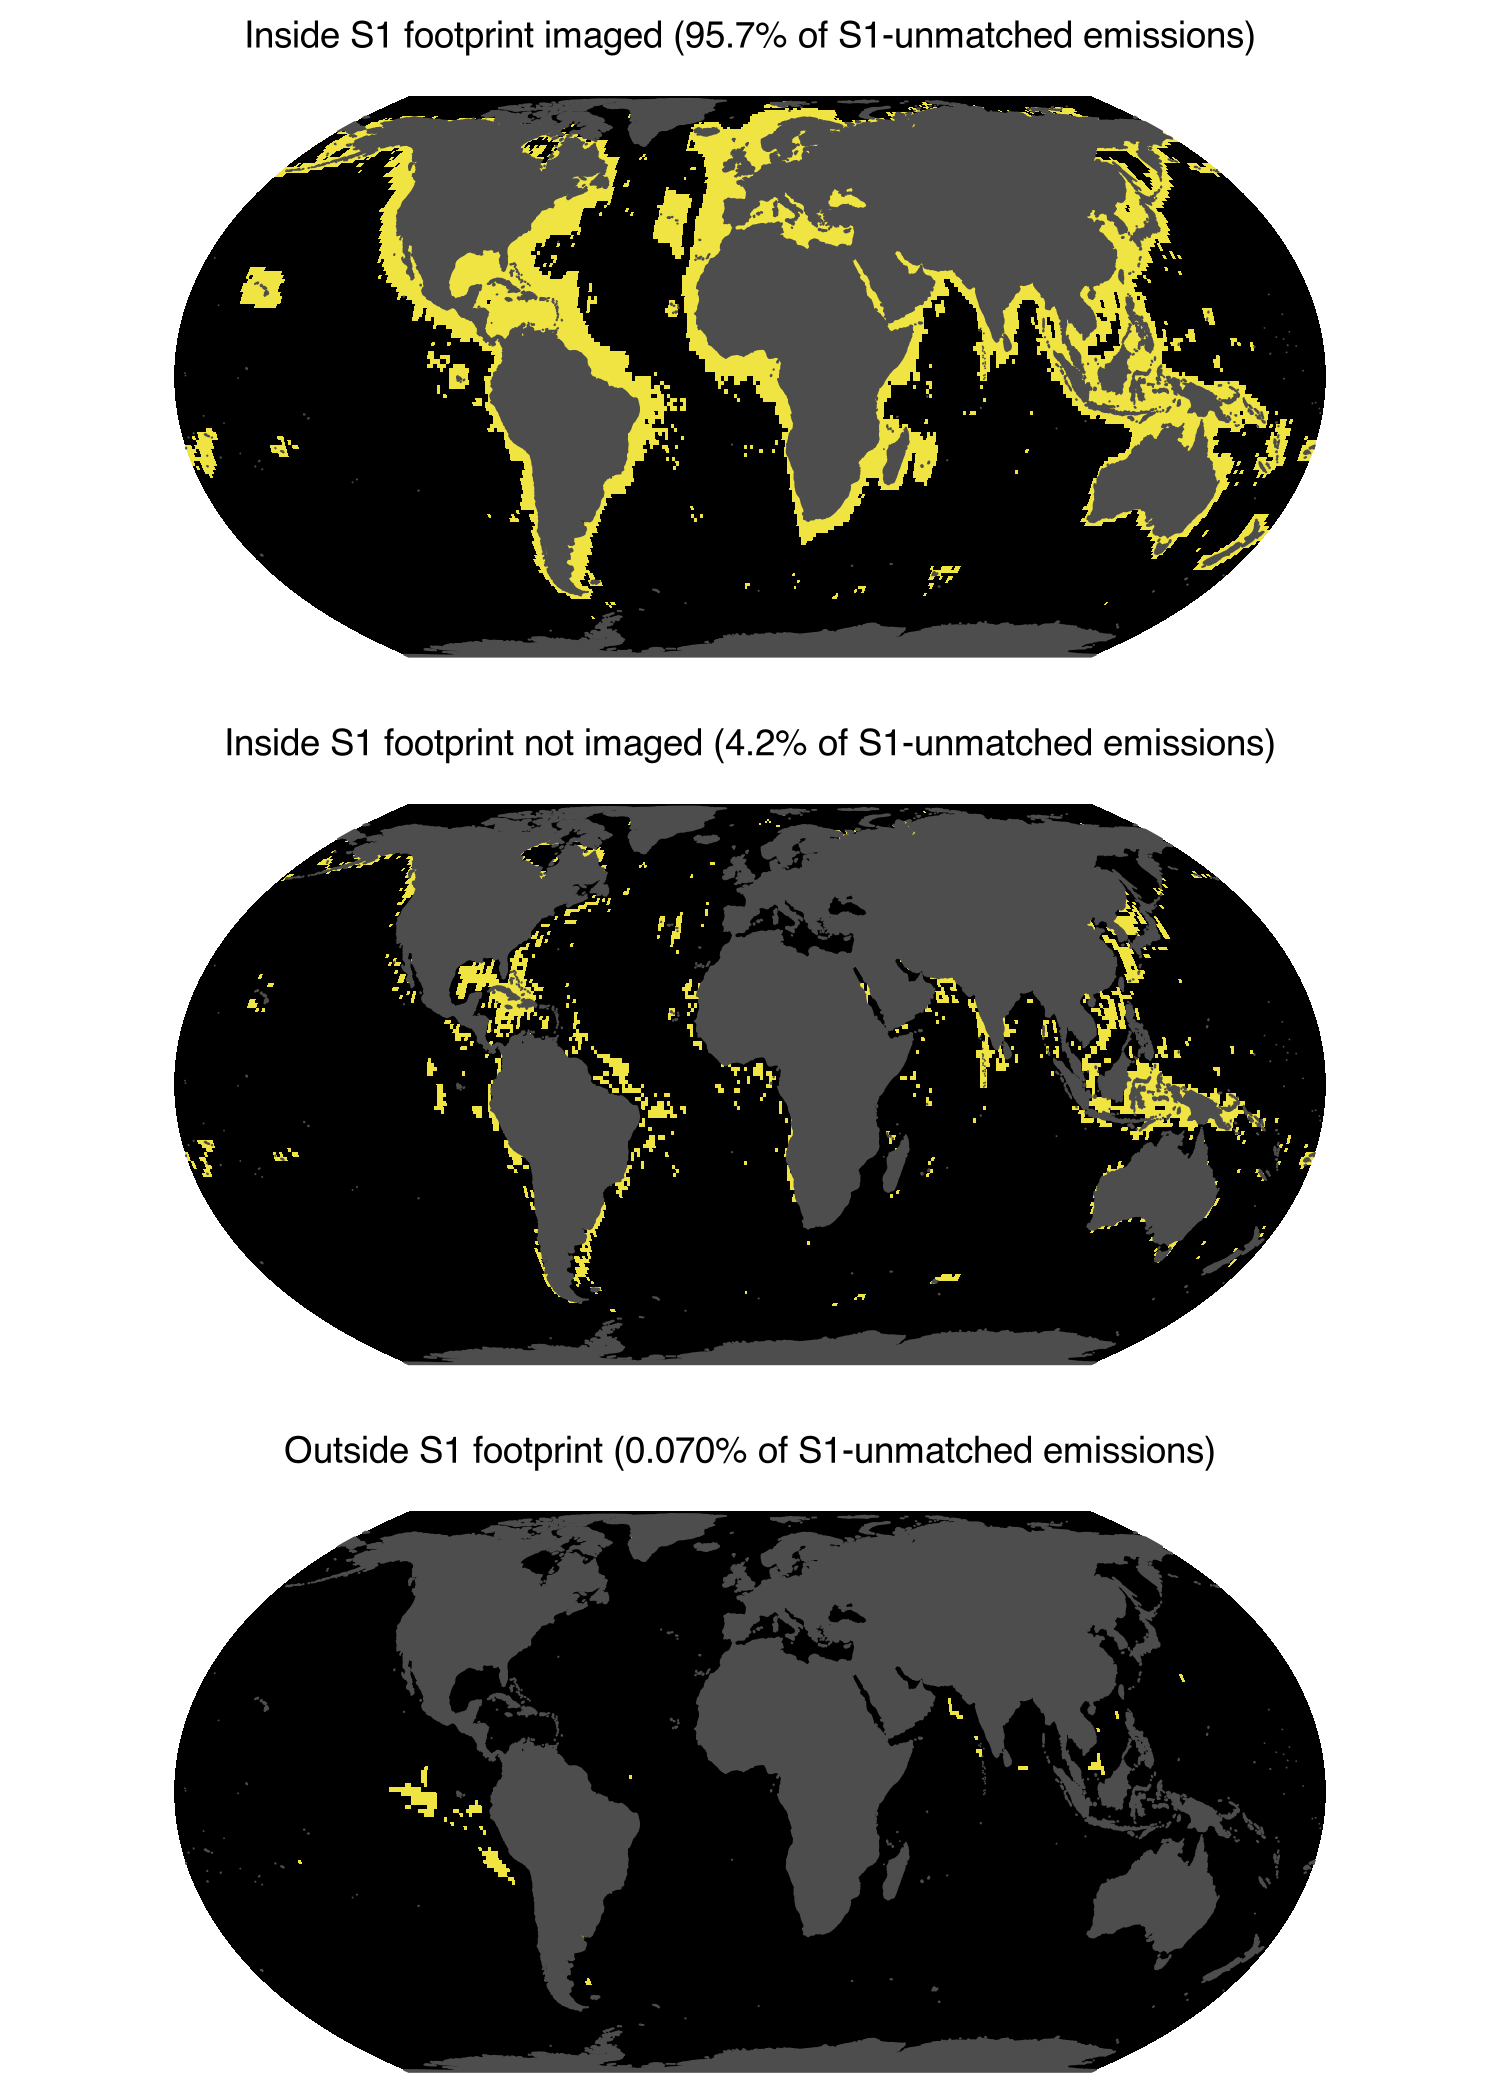
\includegraphics[width=0.8\columnwidth]{figures/fig-spatial-coverage-footprint-1.png}
    \caption{Spatial coverage of the S1-unmatched emissions model. Areas are categorized according to whether they fall inside or outside the S1 footprint and whether they have been imaged by S1 at any point in time. A given pixel may be imaged in some months but not in others. Pixels outside the footprint have never been imaged. The percentage of total S1-unmatched CO$_{2}$ emissions attributed to each category is shown.}
    \label{fig:fig-spatial-coverage-footprint}
\end{figure}

\paragraph{Indirect estimation}

For pixel-months where S1 detections were unavailable, either because they were not imaged due to spatiotemporal satellite heterogeneity or because they fall fully outside the S1 footprint, we first used the detections classification model to predict whether detections were present or absent for each of the length bins and fishing/non-fishing vessel types. If detections were predicted, the subsequent detection regression model was used to predict the density of unmatched S1 detections per unit of S1 sampling effort for each length bin and fishing/non-fishing vessel type. These predicted unmatched detection densities were then fed into the emissions regression model as the separate length-bin-related model features (for each fishing/non-fishing vessel type) to predict the resulting emissions. We do this for all nine emissions regression models corresponding to the three GHGs and six pollutants. Of the total predicted S1-unmatched CO$_2$ emissions, 3.4\% corresponded to indirect estimations within the S1 footprint, while only 0.056\% occurred entirely outside the footprint (Fig. \ref{fig:fig-spatial-coverage-footprint}).



%%%%%%%%%%%%%%%% DATA AND CODE AVAILABILITY %%%%%%%%%%%%%%%
% Nature Communications requires both sections immediately below Methods.

\section*{Data availability}

All data necessary for reproducing this figures and tables in this analysis will be made available in a public GitHub repository with an accompanying Zenodo repository and DOI. It will also be made available in a Code Ocean repository with an accompanying DOI. This section will be updated to include the hyperlinks and DOI upon manuscript acceptance.

\section*{Code availability}

All code necessary for reproducing this figures and tables in this analysis will be made available in a public GitHub repository with an accompanying Zenodo repository and DOI. It will also be made available in a Code Ocean repository with an accompanying DOI. This section will be updated to include the hyperlinks and DOI upon manuscript acceptance.

%%%%%%%%%%%%%%%% REFERENCES %%%%%%%%%%%%%%%

\clearpage 

\bibliography{bibliography}


%%%%%%%%%%%%%%%% BACK MATTER %%%%%%%%%%%%%%%

\section*{Acknowledgments}

We would like to thank the \textit{Nature Communications} editor Bing Xue, along with two anonymous referees, for their constructive feedback on various iterations of this manuscript. The final result was meaningfully shaped by your thought contributions. We would also like to thank the team at Global Fishing Watch, including Camila Vargas Poulsen and Rebecca Stubbs for their help in shepherding this work, and the entire GFW data engineering team for providing the data infrastructure on which so much of this research rests. We would also like to express gratitude to our colleagues at Climate TRACE for their continued support, motivation, and inspiration for developing these data, particularly Gavin McCormick, Lekha Sridhar, and Lauren Betz. We would finally like to thank UCSB's General Research IT (GRIT) team, particularly Michael Colee and Brian Emery, for always supporting our computational and data needs with creativity, deep expertise, speed, and patience.

\section*{Funding}

We gratefully thank Climate TRACE for financially supporting this research. This research also used computational resources provided by the General Research IT (GRIT) group at the University of California, Santa Barbara (primarily supported by the UCSB Office of Research).

\section*{Author contributions statement}
% TODO: Nature Communications asks for one paragraph of descriptive sentences
% rather than the CRediT-style list kept verbatim here.

Conceptualization: GM and DK; Methodology: GM, PCM, OD, EFC, AH, DK,MP, ZW, and CC; Software:  GM, PCM, EFC, AH, and ZW Validation: GM, PCM, DK,MP; Formal analysis: GM, PCM, OD, EFC, AH, DK,MP, ZW, and CC; Investigation: GM, PCM, OD, EFC, AH, DK,MP, ZW, and CC; Data curation:  GM, PCM, EFC, AH, DK,MP and ZW ; Writing - Original Draft: GM, PCM, OD, and CC; Writing -Review \& Editing: GM, PCM, OD, JB, EFC, AH, DK, FSP, MP, ZW, and CC; Visualization: GM and PCM; Supervision: OD, and CC; Project administration: JB; Funding acquisition: GM, PCM, JB, DK, and CC

\section*{Competing interests}

There are no competing interests to declare.

\section*{Use of generative AI}

The authors used a large language model (Anthropic's Claude, through the Claude Code command-line tool) as a programming and editing assistant while preparing this work. As a coding assistant under author direction, we used it to help develop and revise the code for the analysis, as well as the code used to generate figures, tables, and summary statistics. All code is available in the public repository accompanying this paper and is fully reproducible. As an editing assistant under author direction, we used it to draft and edit portions of the manuscript text, primarily in the Methods and Supplementary Information. It was not used to generate or modify any image, figure or map: every figure here is drawn directly from the underlying data by the code in the public repository. It was also not used to modify any table: all tables were generated directly from the underlying data by the code in the public repository. No large language model is listed as an author, and none was used to produce results, to interpret them, or to decide what this paper concludes. All code was reviewed and executed by the authors, and all reported values and statistics are computed from the underlying data by the deposited code. The authors take full responsibility for the content of this article, including any part prepared with the assistance of these tools.


%%%%%%%%%%%%%%%% SUPPLEMENT LIST %%%%%%%%%%%%%%%

% List the contents of your Supplementary Materials, including the numbers of any
% supplementary figures, tables, external data files etc. and any references that are
% cited only in the supplement. In this example, refs. 7-8 are cited only in the supplement.
% Fill out your numbers accordingly and delete any lines that aren't applicable.


%%%%%%%%%%%%%%%% END OF MAIN TEXT %%%%%%%%%%%%%%%

\newpage

%%%%%%%%%%%%%%%% START OF SUPPLEMENT %%%%%%%%%%%%%%%

% Nature Communications style: display items restart at 1 and are labelled
% "Supplementary Figure 1" / "Supplementary Table 1"; text sections are
% "Supplementary Note 1" etc. Cite them as Supplementary Fig. / Table / Note N.
% Equations and pages keep the S prefix.
\renewcommand{\thefigure}{\arabic{figure}}
\renewcommand{\thetable}{\arabic{table}}
\renewcommand{\figurename}{Supplementary Figure}
\renewcommand{\tablename}{Supplementary Table}
\newcounter{supnote}
\newcommand{\supnote}[2]{\refstepcounter{supnote}\label{#2}\subsection*{Supplementary Note \thesupnote: #1}}
\renewcommand{\theequation}{S\arabic{equation}}
\renewcommand{\thepage}{S\arabic{page}}
\setcounter{figure}{0}
\setcounter{table}{0}
\setcounter{equation}{0}
\setcounter{page}{1} % not 0 as \newpage already started a supplementary page
% References continue the numbering from the main text.

% Restarting the counters above also restarts the names hyperref builds its PDF
% anchors from: those come from \theH<counter>, not from \the<counter>, so the
% S prefix added above does not reach them. Without these lines Fig. S16 asks
% for the anchor "figure.16" that main-text Fig. 16 already claimed, pdfTeX
% drops the duplicate, and the supplementary link lands on the main-text float
% carrying the same number. Nothing here is printed; it only names the targets.
\providecommand{\theHfigure}{\arabic{figure}}
\providecommand{\theHtable}{\arabic{table}}
\providecommand{\theHequation}{\arabic{equation}}
\renewcommand{\theHfigure}{S\arabic{figure}}
\renewcommand{\theHtable}{S\arabic{table}}
\renewcommand{\theHequation}{S\arabic{equation}}


%%%%%%%%%%%%%%%% SUPPLEMENT TITLE PAGE %%%%%%%%%%%%%%%

\begin{center}
\section*{Supplementary Materials for\\ Quantifying comprehensive marine vessel emissions using satellite data fusion}

\author{
	% You can write out first names or use initials - either way is acceptable, but be consistent
	Gavin~McDonald$^\ast$,
    Pol~Carbó-Mestre,
    Olivier~Deschenes,
    Jennifer~Bone,
    E.~Fernando~Cagua,
    Anna~Hughes,
    David~Kroodsma,
    Fernando~S.~Paolo,
    Mark~Powell,
	Zihan~Wei,
    Christopher~Costello
	\small$^\ast$Corresponding author. Email: gmcdonald@bren.ucsb.edu}
\end{center}

\subsubsection*{This PDF file includes:}
\begin{itemize}
    \item Supplementary Figures 1 to 15
    \item Supplementary Tables 1 to 8
    \item Supplementary Notes 1 to 3
\end{itemize}

\subsubsection*{Other Supplementary Materials for this manuscript include the following:}
\begin{itemize}
    \item Supplementary Data 1 to 3 (CSV files; described below)
\end{itemize}

\subsubsection*{Supplementary Figures}
\begin{itemize}\setlength{\itemsep}{0pt}
    \item[1.] Fishing and non-fishing components of the global emissions time series and maps (p.~\pageref{fig:fig-spatial-temporal-richness-by-fleet-total-pseudolog})
    \item[2.] Spatial maps of 2025 emissions for each GHG and pollutant (p.~\pageref{fig:fig-pollutant-maps})
    \item[3.] Monthly global emissions time series for each GHG and pollutant (p.~\pageref{fig:fig-pollutant-time-series})
    \item[4.] CO$_{2}$ emissions by country and activity type for AIS-broadcasting vessels, 2025 (p.~\pageref{fig:fig-emissions-by-country-and-activity-type})
    \item[5.] Trend in CO$_{2}$ emissions by ocean, normalized to the 2017 baseline (p.~\pageref{fig:fig-emissions-marine-ocean-other})
    \item[6.] Annual CO$_{2}$ emissions by ocean and data source (p.~\pageref{fig:fig-annual-emissions-by-ocean-and-data-source})
    \item[7.] Passenger vessels by length bin, 2017 against 2025 (p.~\pageref{fig:figS-passenger-size-panels})
    \item[8.] Fleet composition in 2025: share of the fleet against share of CO$_{2}$ by vessel class (p.~\pageref{fig:figS-fleet-sankey-with-series-2025})
    \item[9.] Annual CO$_{2}$ emissions, AIS messages and vessel counts by AIS receiver type (p.~\pageref{fig:fig-annual-emissions-by-ais-receiver-type})
    \item[10.] Annual CO$_{2}$ emissions by AIS receiver type for the ten highest-emitting flags (p.~\pageref{fig:fig-annual-emissions-by-ais-receiver-type-top-flags})
    \item[11.] Spatial change in CO$_{2}$ emissions between 2017 and 2025 by AIS receiver type (p.~\pageref{fig:fig-co2-emissions-change-map-by-receiver-type})
    \item[12.] Trends in our AIS-based and fused estimates against other inventories (p.~\pageref{fig:figS-inventory-comparison-all-sources})
    \item[13.] AIS carriage saturation by vessel size (p.~\pageref{fig:figS-ais-carriage-saturation-by-size})
    \item[14.] S1 detection density by length bin and AIS match status (p.~\pageref{fig:figS-density-by-match-status})
\end{itemize}

\subsubsection*{Supplementary Tables}
\begin{itemize}\setlength{\itemsep}{0pt}
    \item[1.] 2017 and 2025 emissions by data source and pollutant (p.~\pageref{tab:total_percent_change_by_fleet})
    \item[2.] AIS-only underestimation of 2025 emissions and overestimation of the 2017 to 2025 trend, by pollutant (p.~\pageref{tab:pollutant_ais_underestimation_overestimation_summary})
    \item[3.] 2025 CO$_{2}$ emissions by ocean (p.~\pageref{tab:emissions_by_ocean_summary_tbl})
    \item[4.] Emissions and social cost of each GHG for fishing and non-fishing vessels (p.~\pageref{tab:social_cost_summary_tbl})
    \item[5.] Top 30 countries by 2025 CO$_{2}$ emissions from AIS-broadcasting vessels, by activity type (p.~\pageref{tab:top_countries_by_activity_type})
    \item[6.] Annual CO$_{2}$ emissions: our estimates against the published bottom-up inventories (p.~\pageref{tab:inventory_comparison_all_sources})
    \item[7.] Annual CO$_{2}$ emissions: our estimates against the shipping sector of EDGAR and CEDS (p.~\pageref{tab:multisector_shipping_comparison})
    \item[8.] Growth in CO$_{2}$ emissions, as total change and compound annual growth rate, for our estimates and every inventory compared (p.~\pageref{tab:inventory_growth_comparison})
\end{itemize}

\subsubsection*{Supplementary Notes}
\begin{itemize}\setlength{\itemsep}{0pt}
    \item[1.] Trends in AIS receiver types (p.~\pageref{sec:ais-receiver-types})
    \item[2.] Systematic comparison of our AIS-based emissions modeling methodology to other AIS-based inventories (p.~\pageref{sec:methods-comparison})
    \item[3.] Systematic comparison of our emissions magnitude and trend estimates to other inventories (p.~\pageref{sec:inventory-comparison})
\end{itemize}

\subsubsection*{Supplementary Data}
Comparison of our AIS-based emissions inventory with six published bottom-up, activity-based inventories (STEAM, SEIM, MariTEAM, OECD, SAVE and the Fourth IMO GHG Study), one column per inventory. Referenced in Supplementary Note 2.
\begin{itemize}\setlength{\itemsep}{0pt}
    \item[1.] \path{bottom-up_inventory_comparison_methods.csv}. Methodology: main engine power and engine types, fuel types, main engine correction factors, specific fuel oil consumption, low-load adjustment, auxiliary engine and boiler power, emission control areas, imputation for vessels without AIS data, and validation.
    \item[2.] \path{bottom-up_inventory_comparison_inputs.csv}. Input data: AIS receiver types, vessel-characteristics sources, spatial and temporal coverage, number of vessels, and number of AIS messages after processing.
    \item[3.] \path{bottom-up_inventory_comparison_outputs.csv}. Inventory outputs: pollutants and other outputs, spatial and temporal resolution, disaggregation dimensions, and data access.
\end{itemize}

\newpage
%%%%%%%%%%%%%%%% SUPPLEMENTARY FIGURES, TABLES AND NOTES %%%%%%%%%%%%%%%

\section*{Supplementary Figures}

\begin{figure}[H]
    \centering
    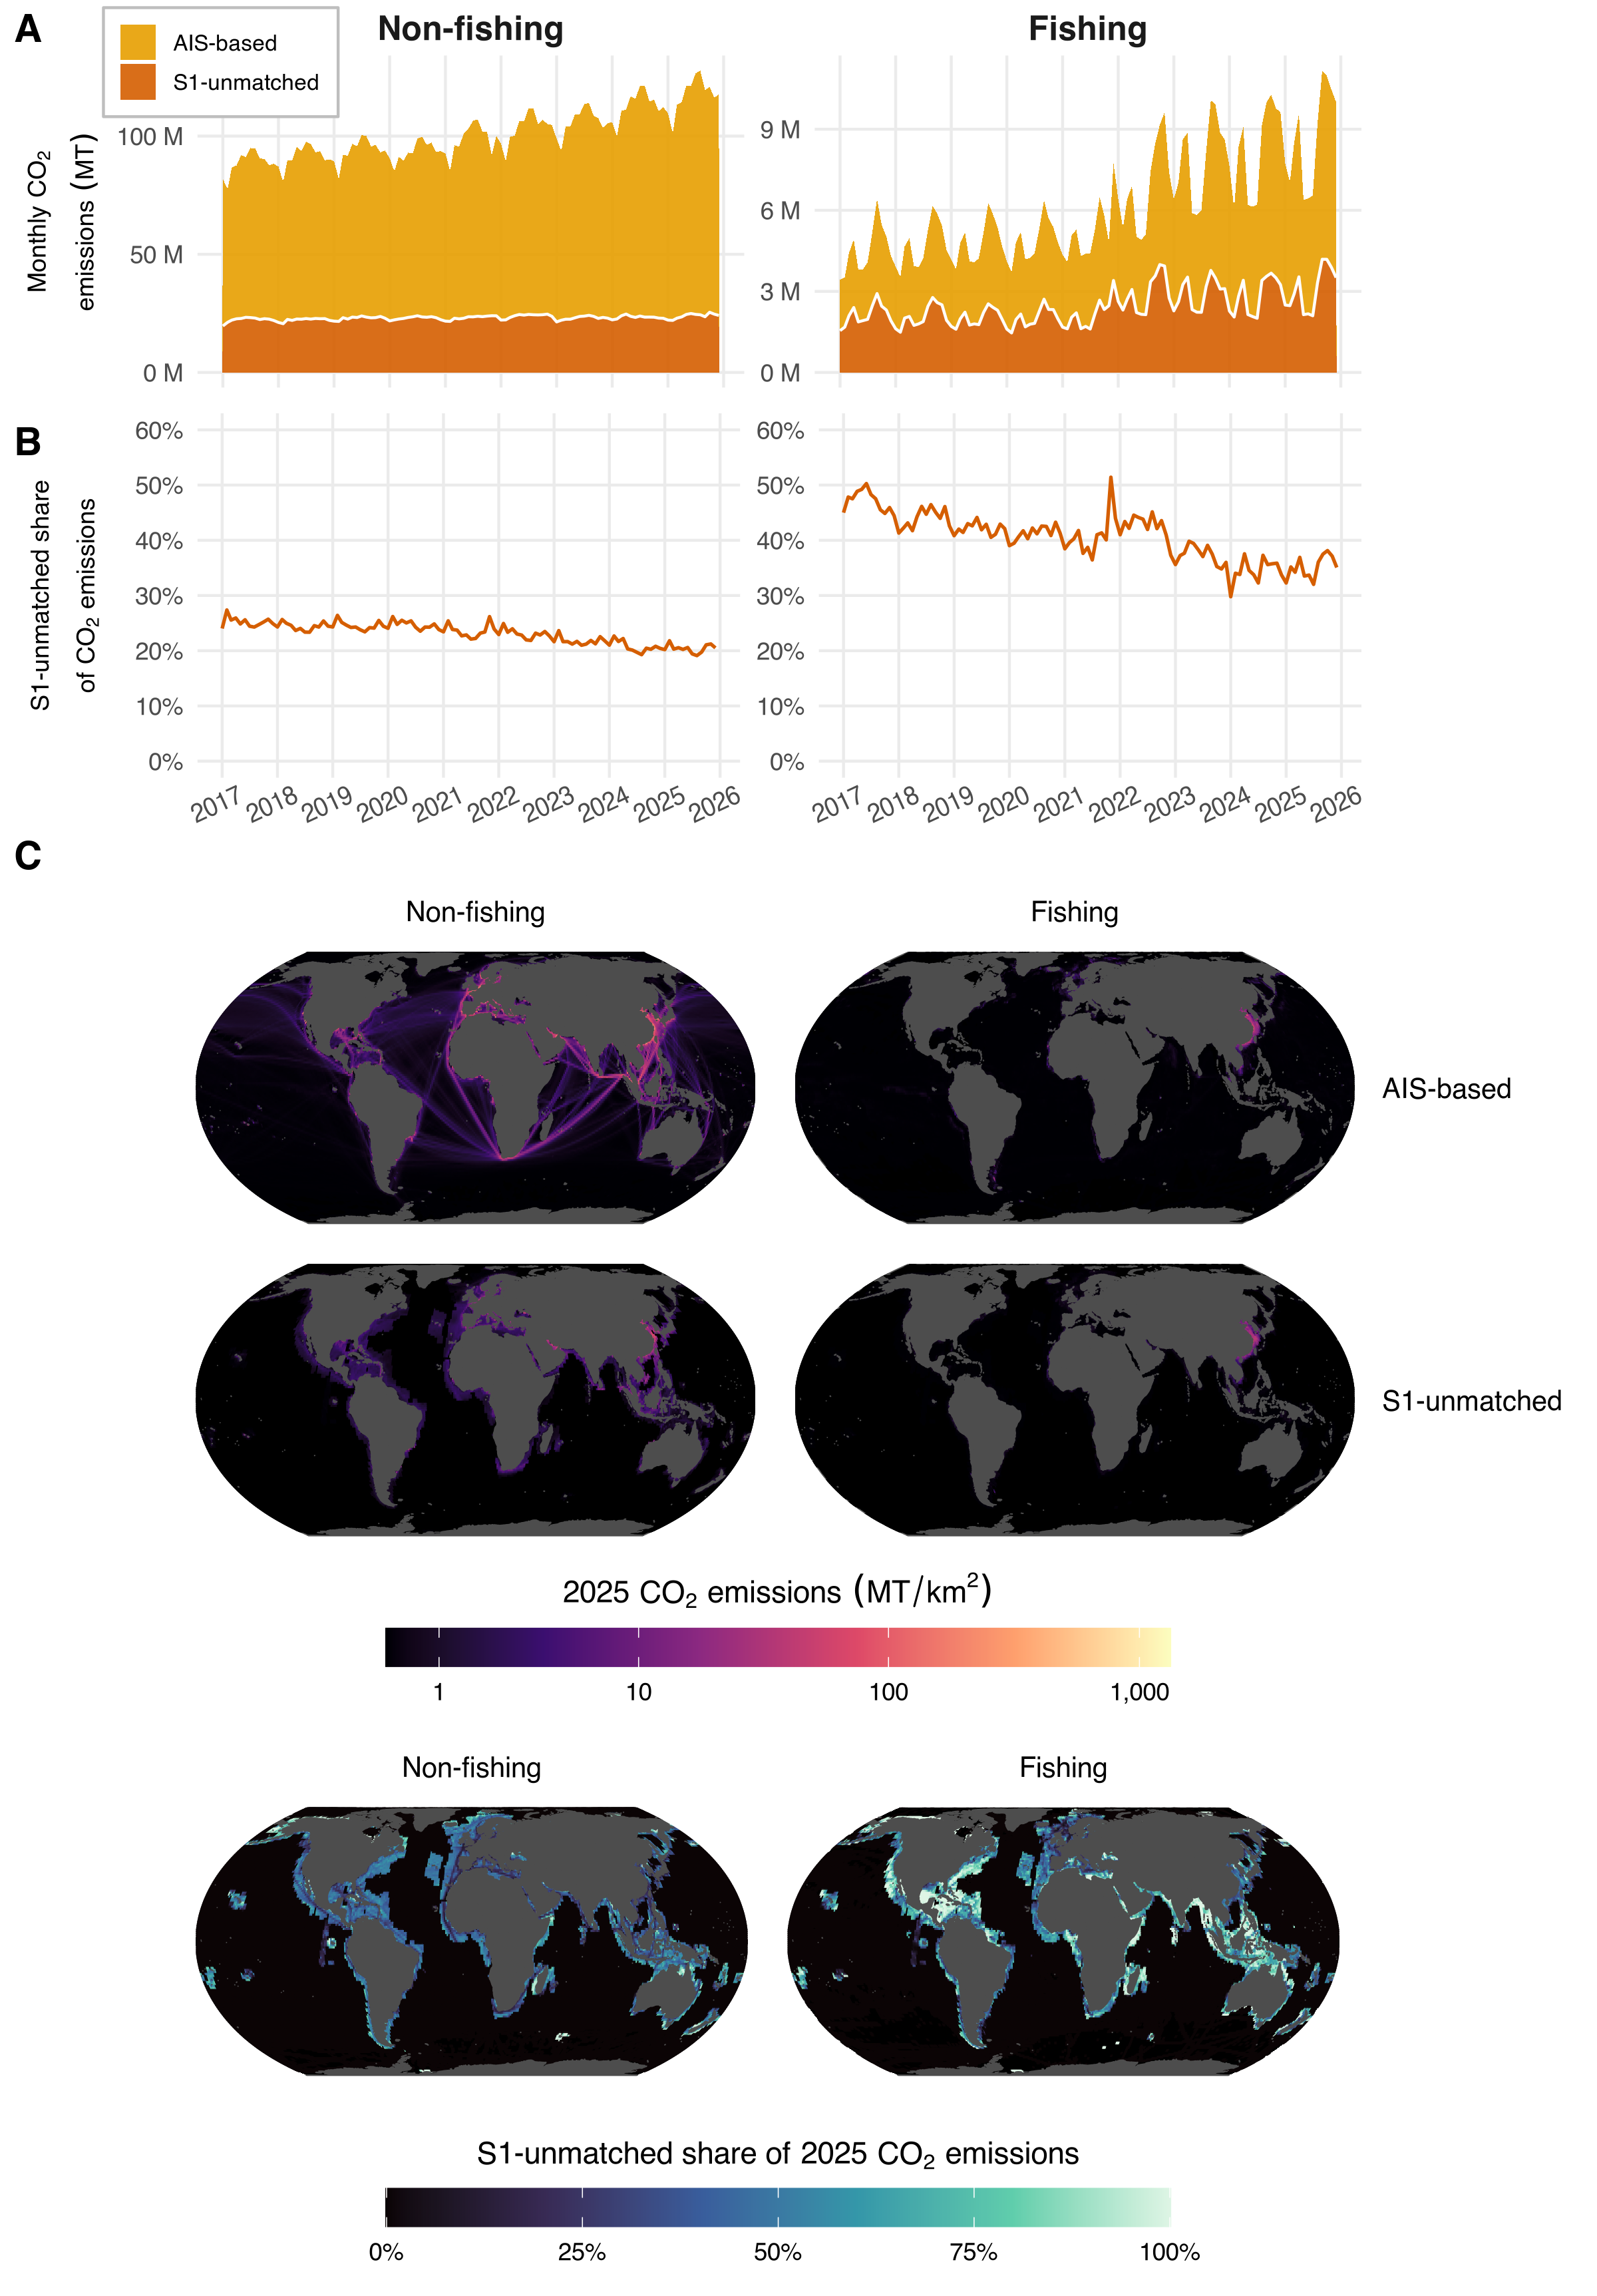
\includegraphics[width=\columnwidth]{figures/fig-spatial-temporal-richness-by-fleet-total-pseudolog-1.png}
    \caption{The fishing and non-fishing components of Figure \ref{fig:fig-emissions-time-series-and-maps}, panel for panel. (a) Time series of monthly global CO$_2$ emissions, shown for both AIS-based and S1-unmatched emissions, and for both fishing and non-fishing vessels. (b) Time series of the monthly share of global CO$_{2}$ emissions that is S1-unmatched, for both fishing and non-fishing vessels. (c) Spatial distribution of 2025 CO$_{2}$ emissions, AIS-based (top) and S1-unmatched (middle), for both fishing and non-fishing vessels (columns), shown at a 1x1 degree spatial resolution; emissions are area-normalized for each pixel (metric tonnes per square kilometer, shown on a pseudolog-10 scale). The bottom maps show, for each pixel, the share of its 2025 CO$_{2}$ emissions from that group of vessels that is S1-unmatched; unlike the maps above them this is a bounded percentage rather than a magnitude, so it carries its own color scale. Pixels with no 2025 emissions from the group in question have no share to show and are drawn in the background color, as are pixels with no emissions on the maps above.}
    \label{fig:fig-spatial-temporal-richness-by-fleet-total-pseudolog}
\end{figure}

\begin{figure}[H]
    \centering
    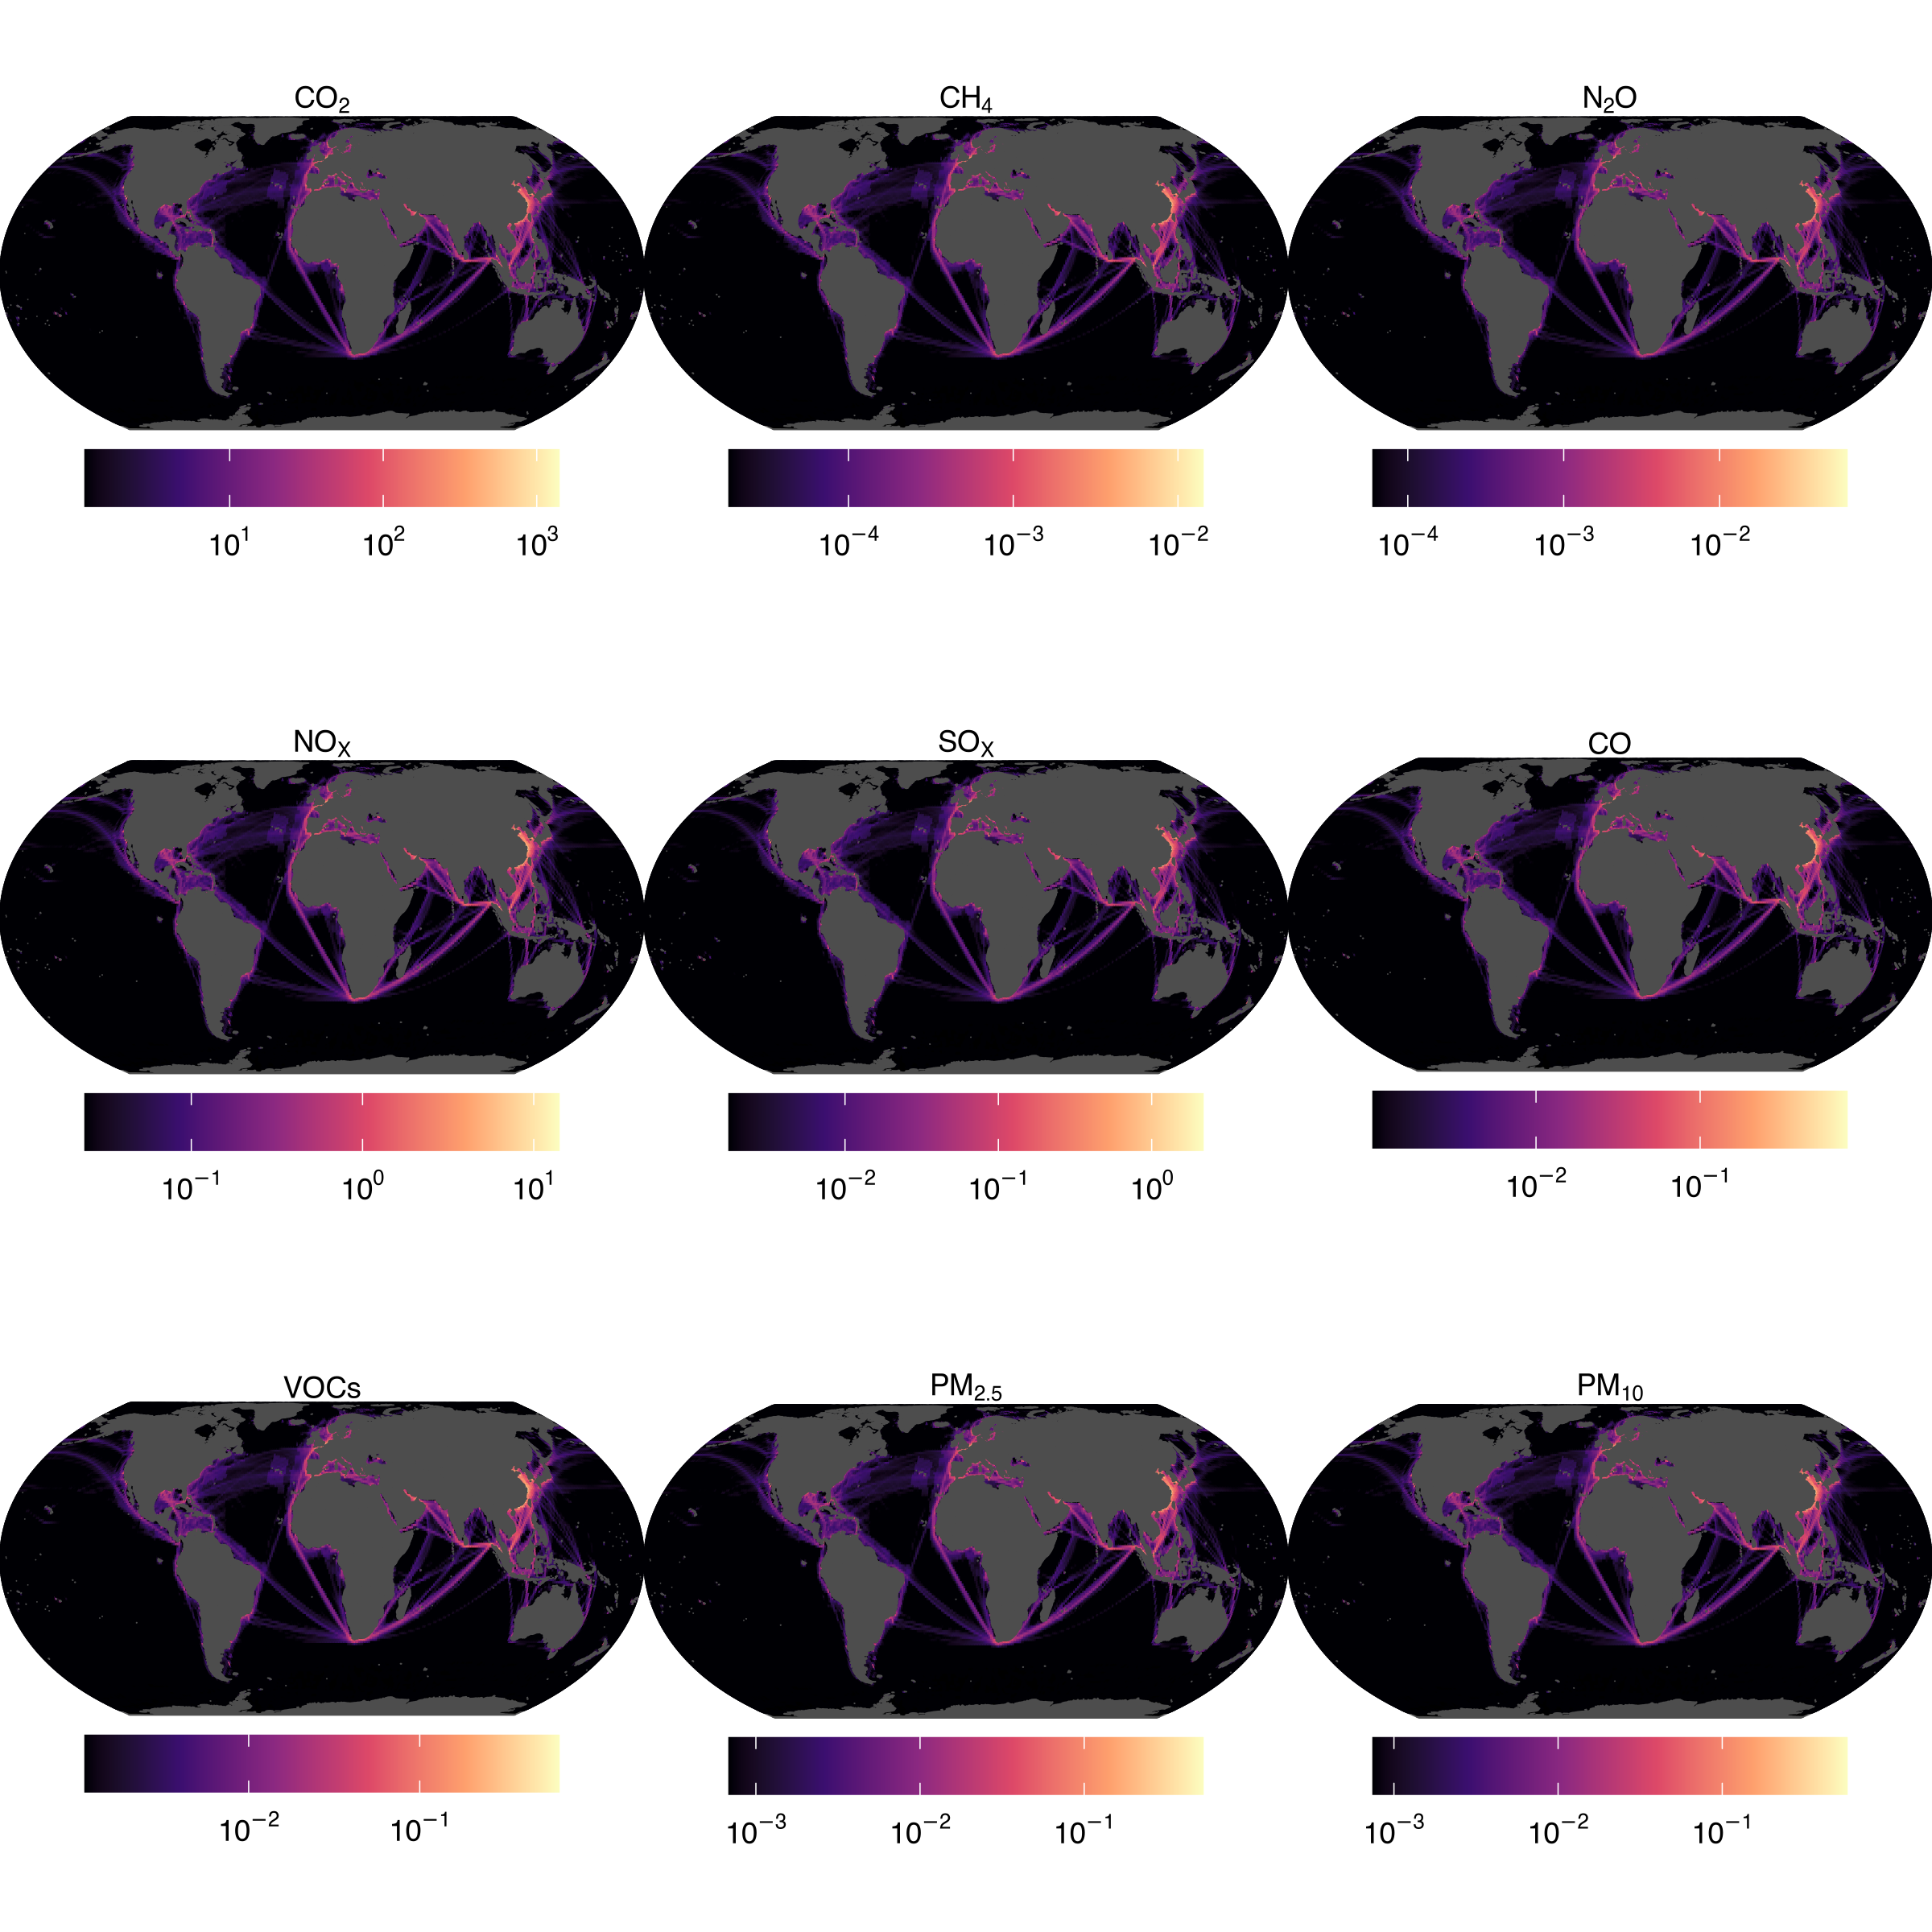
\includegraphics[width=\columnwidth]{figures/fig-pollutant-maps-qlog10-1.png}
    \caption{Spatial maps of 2025 emissions for each GHG and pollutant, aggregated across AIS-based and S1-unmatched emissions, and shown at a 1x1 degree spatial resolution. Emissions are area-normalized for each pixel (metric tonnes per square kilometer) and shown using a log-10 scale. Each panel is scaled independently, spanning the 75th percentile to the maximum of that pollutant, with lower values drawn in the darkest color; colors are therefore not comparable between panels.}
    \label{fig:fig-pollutant-maps}
\end{figure}

\begin{figure}[H]
    \centering
    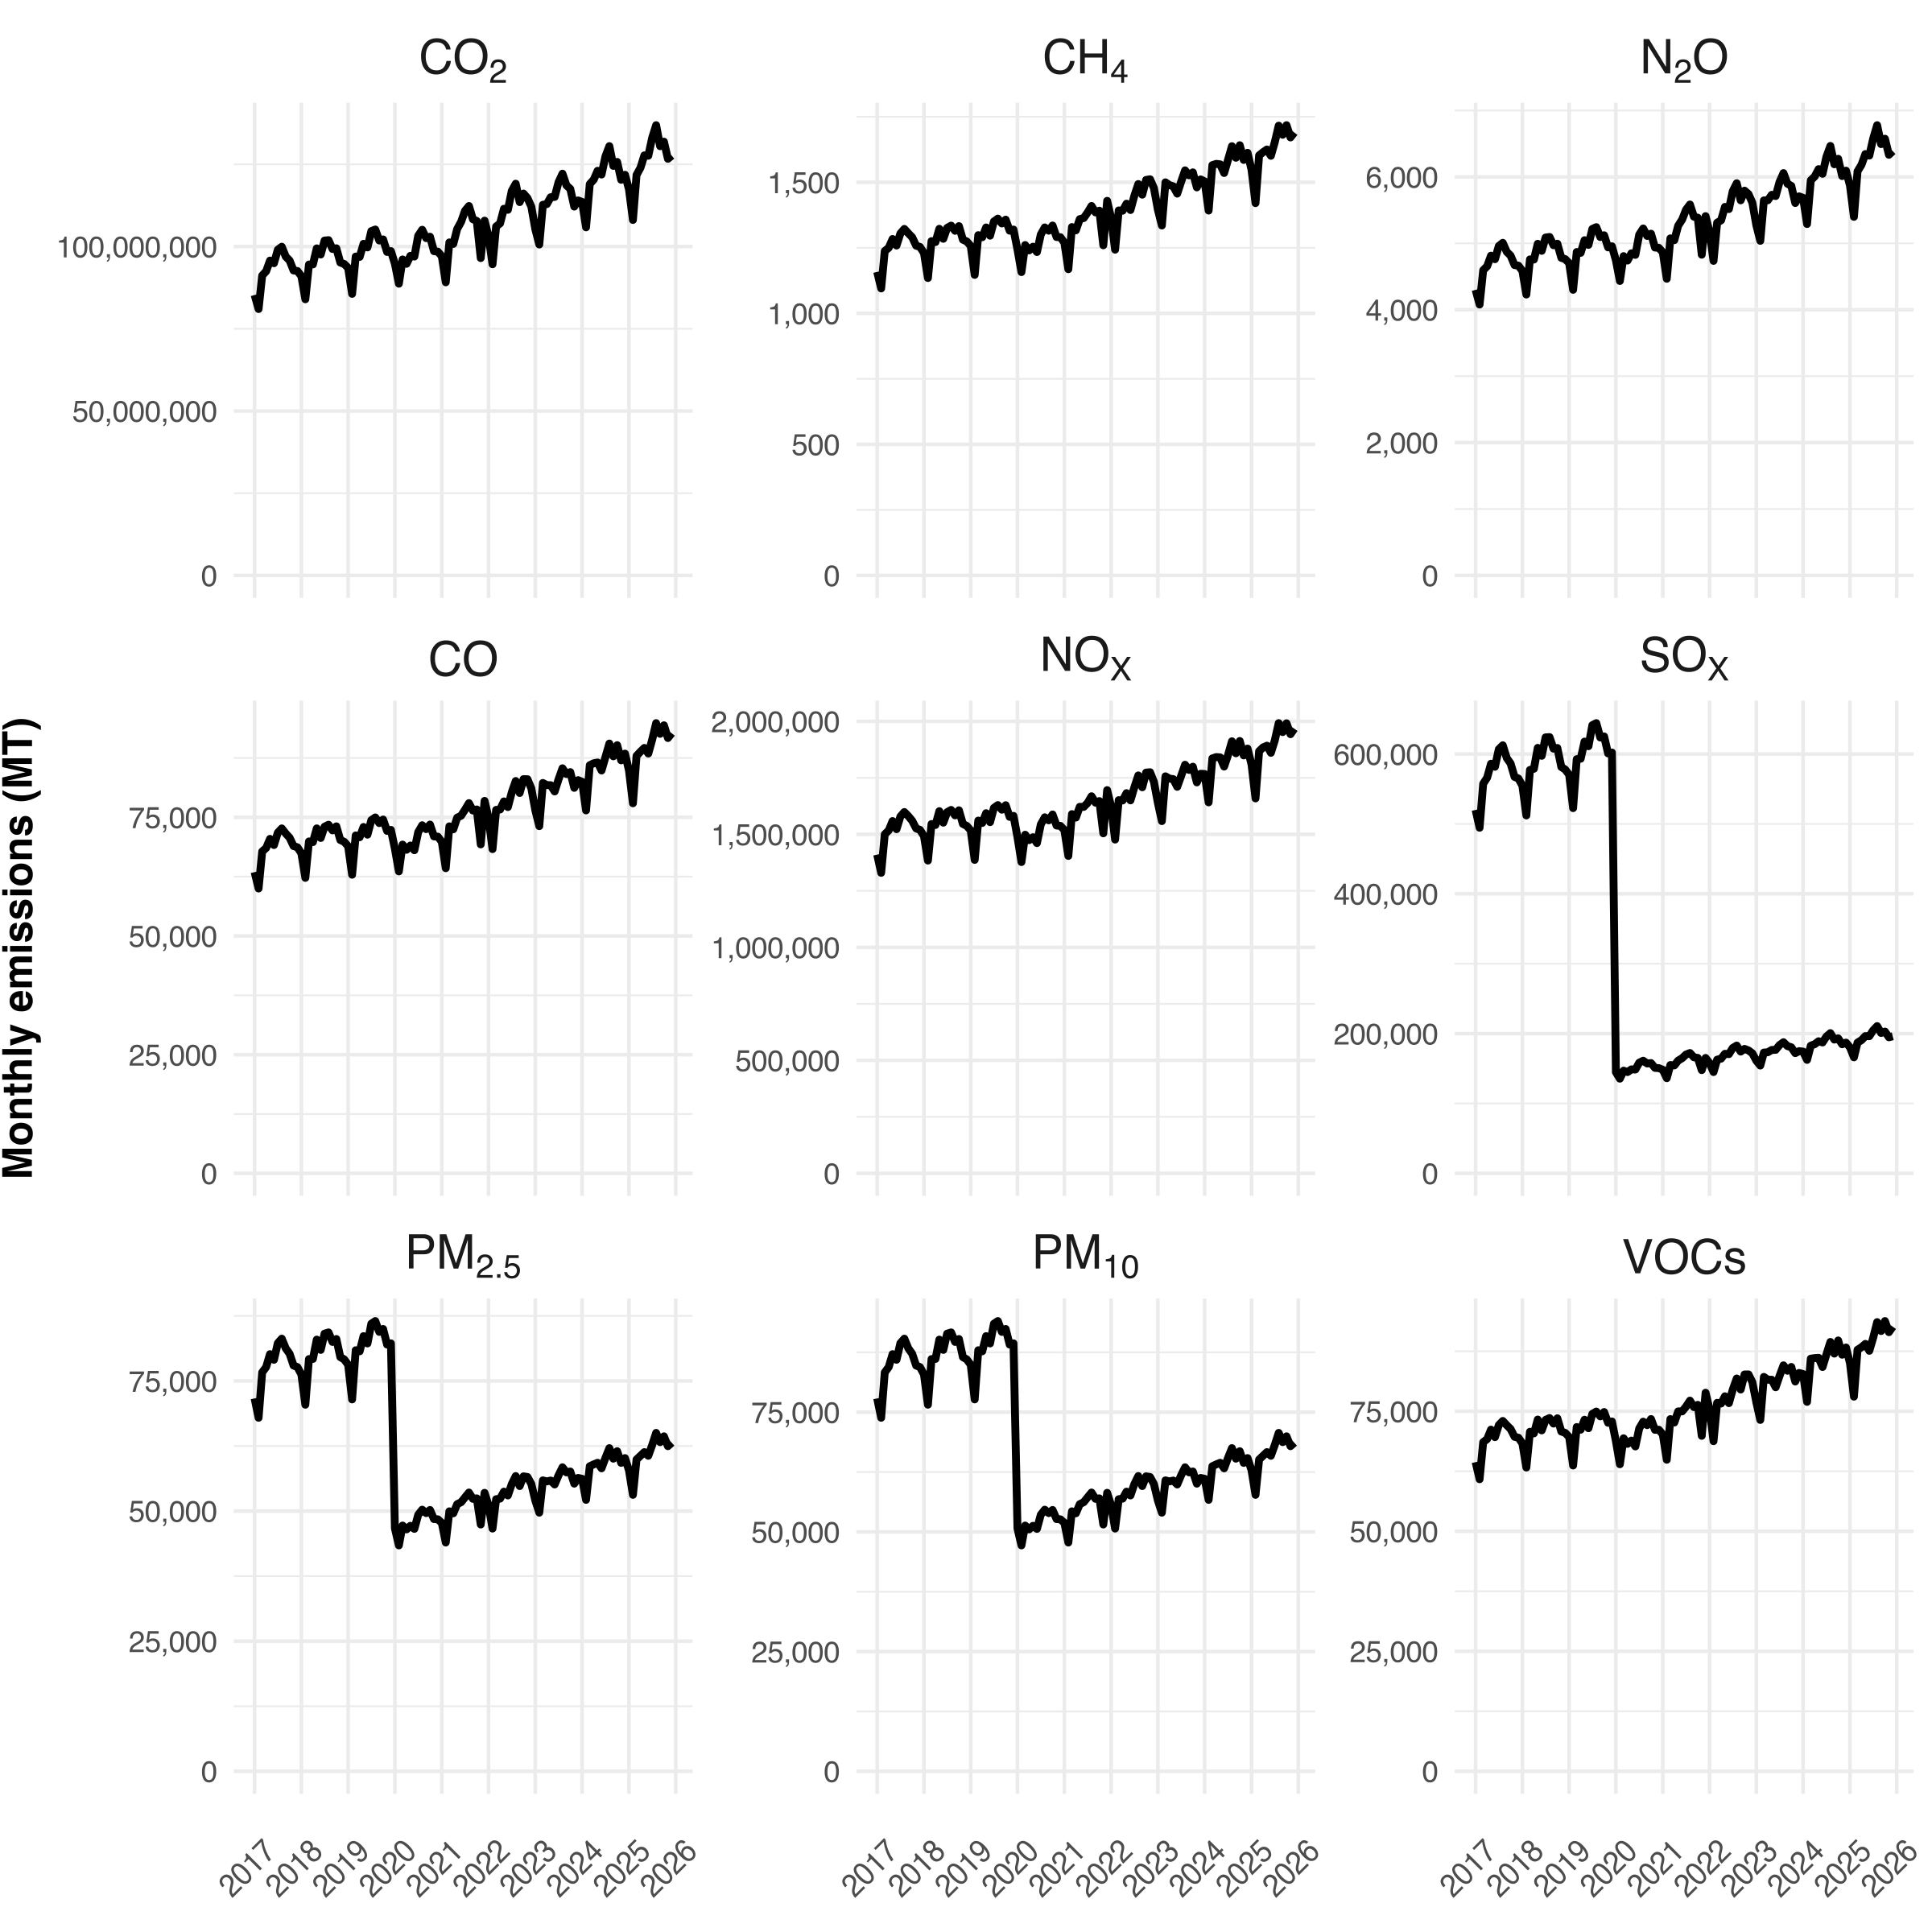
\includegraphics[width=\columnwidth]{figures/fig-pollutant-time-series-1.png}
    \caption{Time series of monthly global emissions for each GHG and pollutant, aggregated across AIS-based and S1-unmatched emissions.}
    \label{fig:fig-pollutant-time-series}
\end{figure}

\begin{figure}[H]
    \centering
    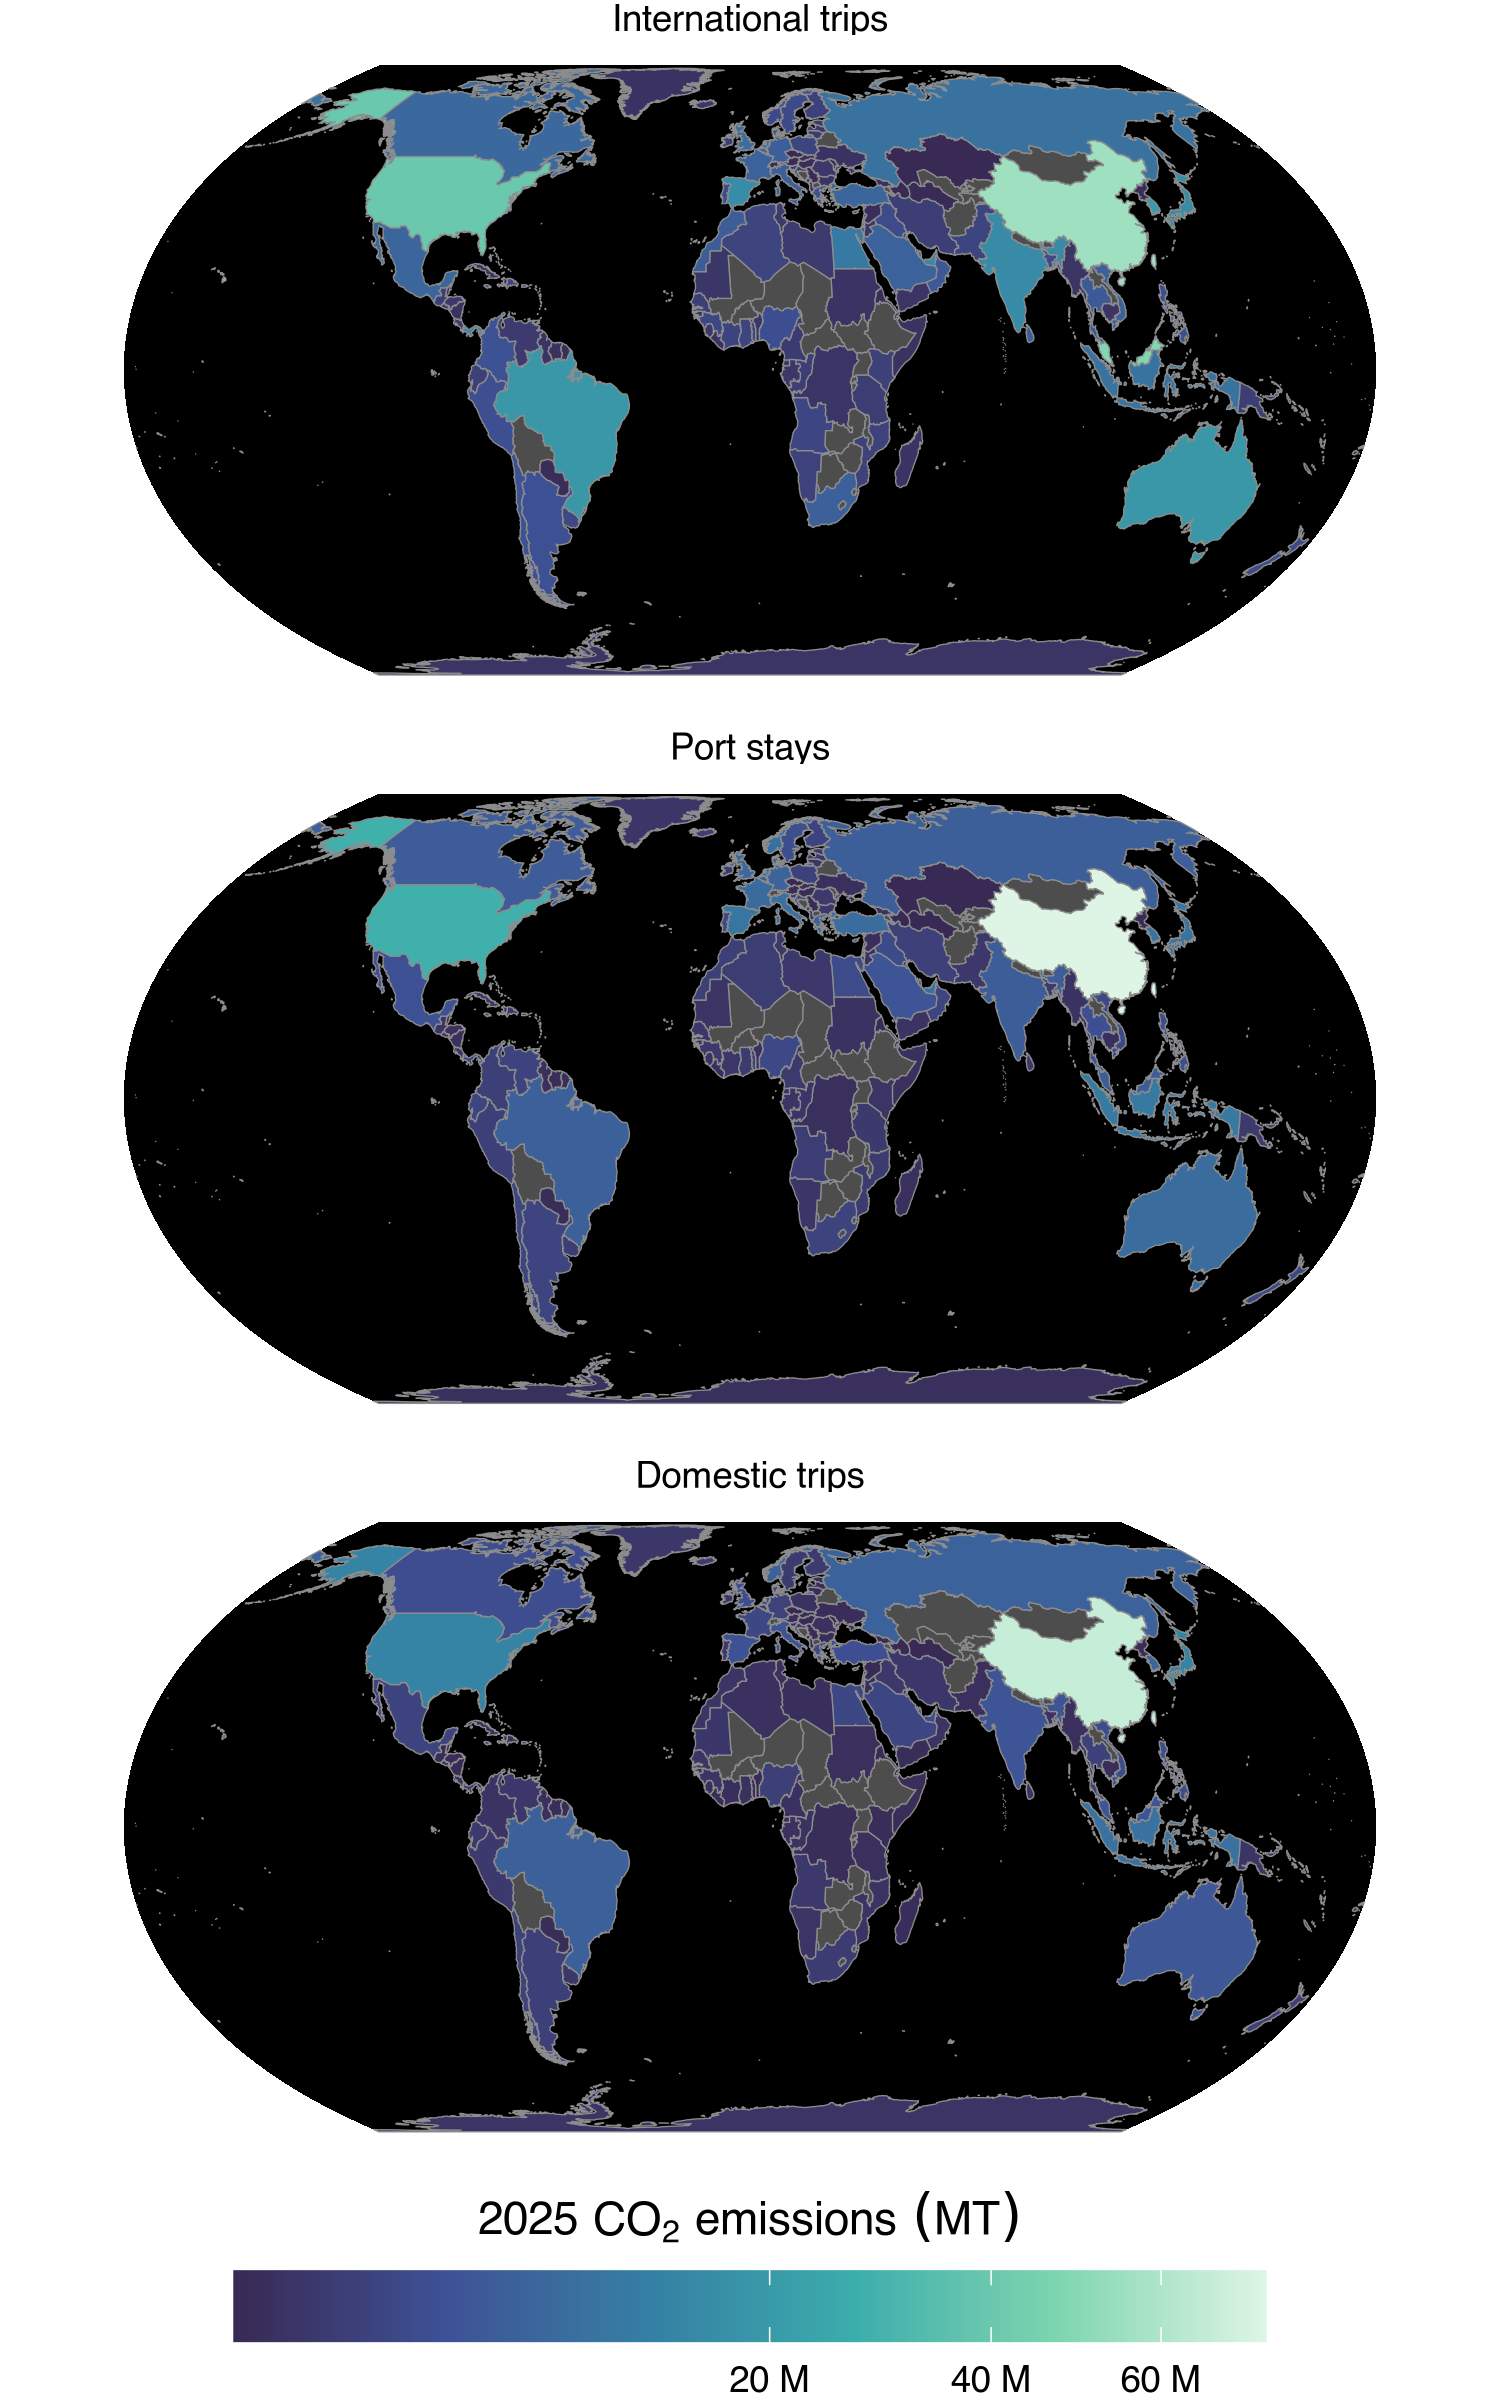
\includegraphics[width=0.85\columnwidth]{figures/fig-emissions-by-country-and-activity-type-1.png}
    \caption{CO$_{2}$ emissions by country for AIS-broadcasting vessels during different activity types (international trips, port stays, and domestic trips), aggregated for activities ending in 2025. Emissions for each international trip are partitioned equally to its departure and arrival country. The color scale is square-root transformed, so that lower-emitting countries remain distinguishable alongside the largest emitters. Countries with no values are shown in gray.}
    \label{fig:fig-emissions-by-country-and-activity-type}
\end{figure}

\begin{figure}[H]
    \centering
    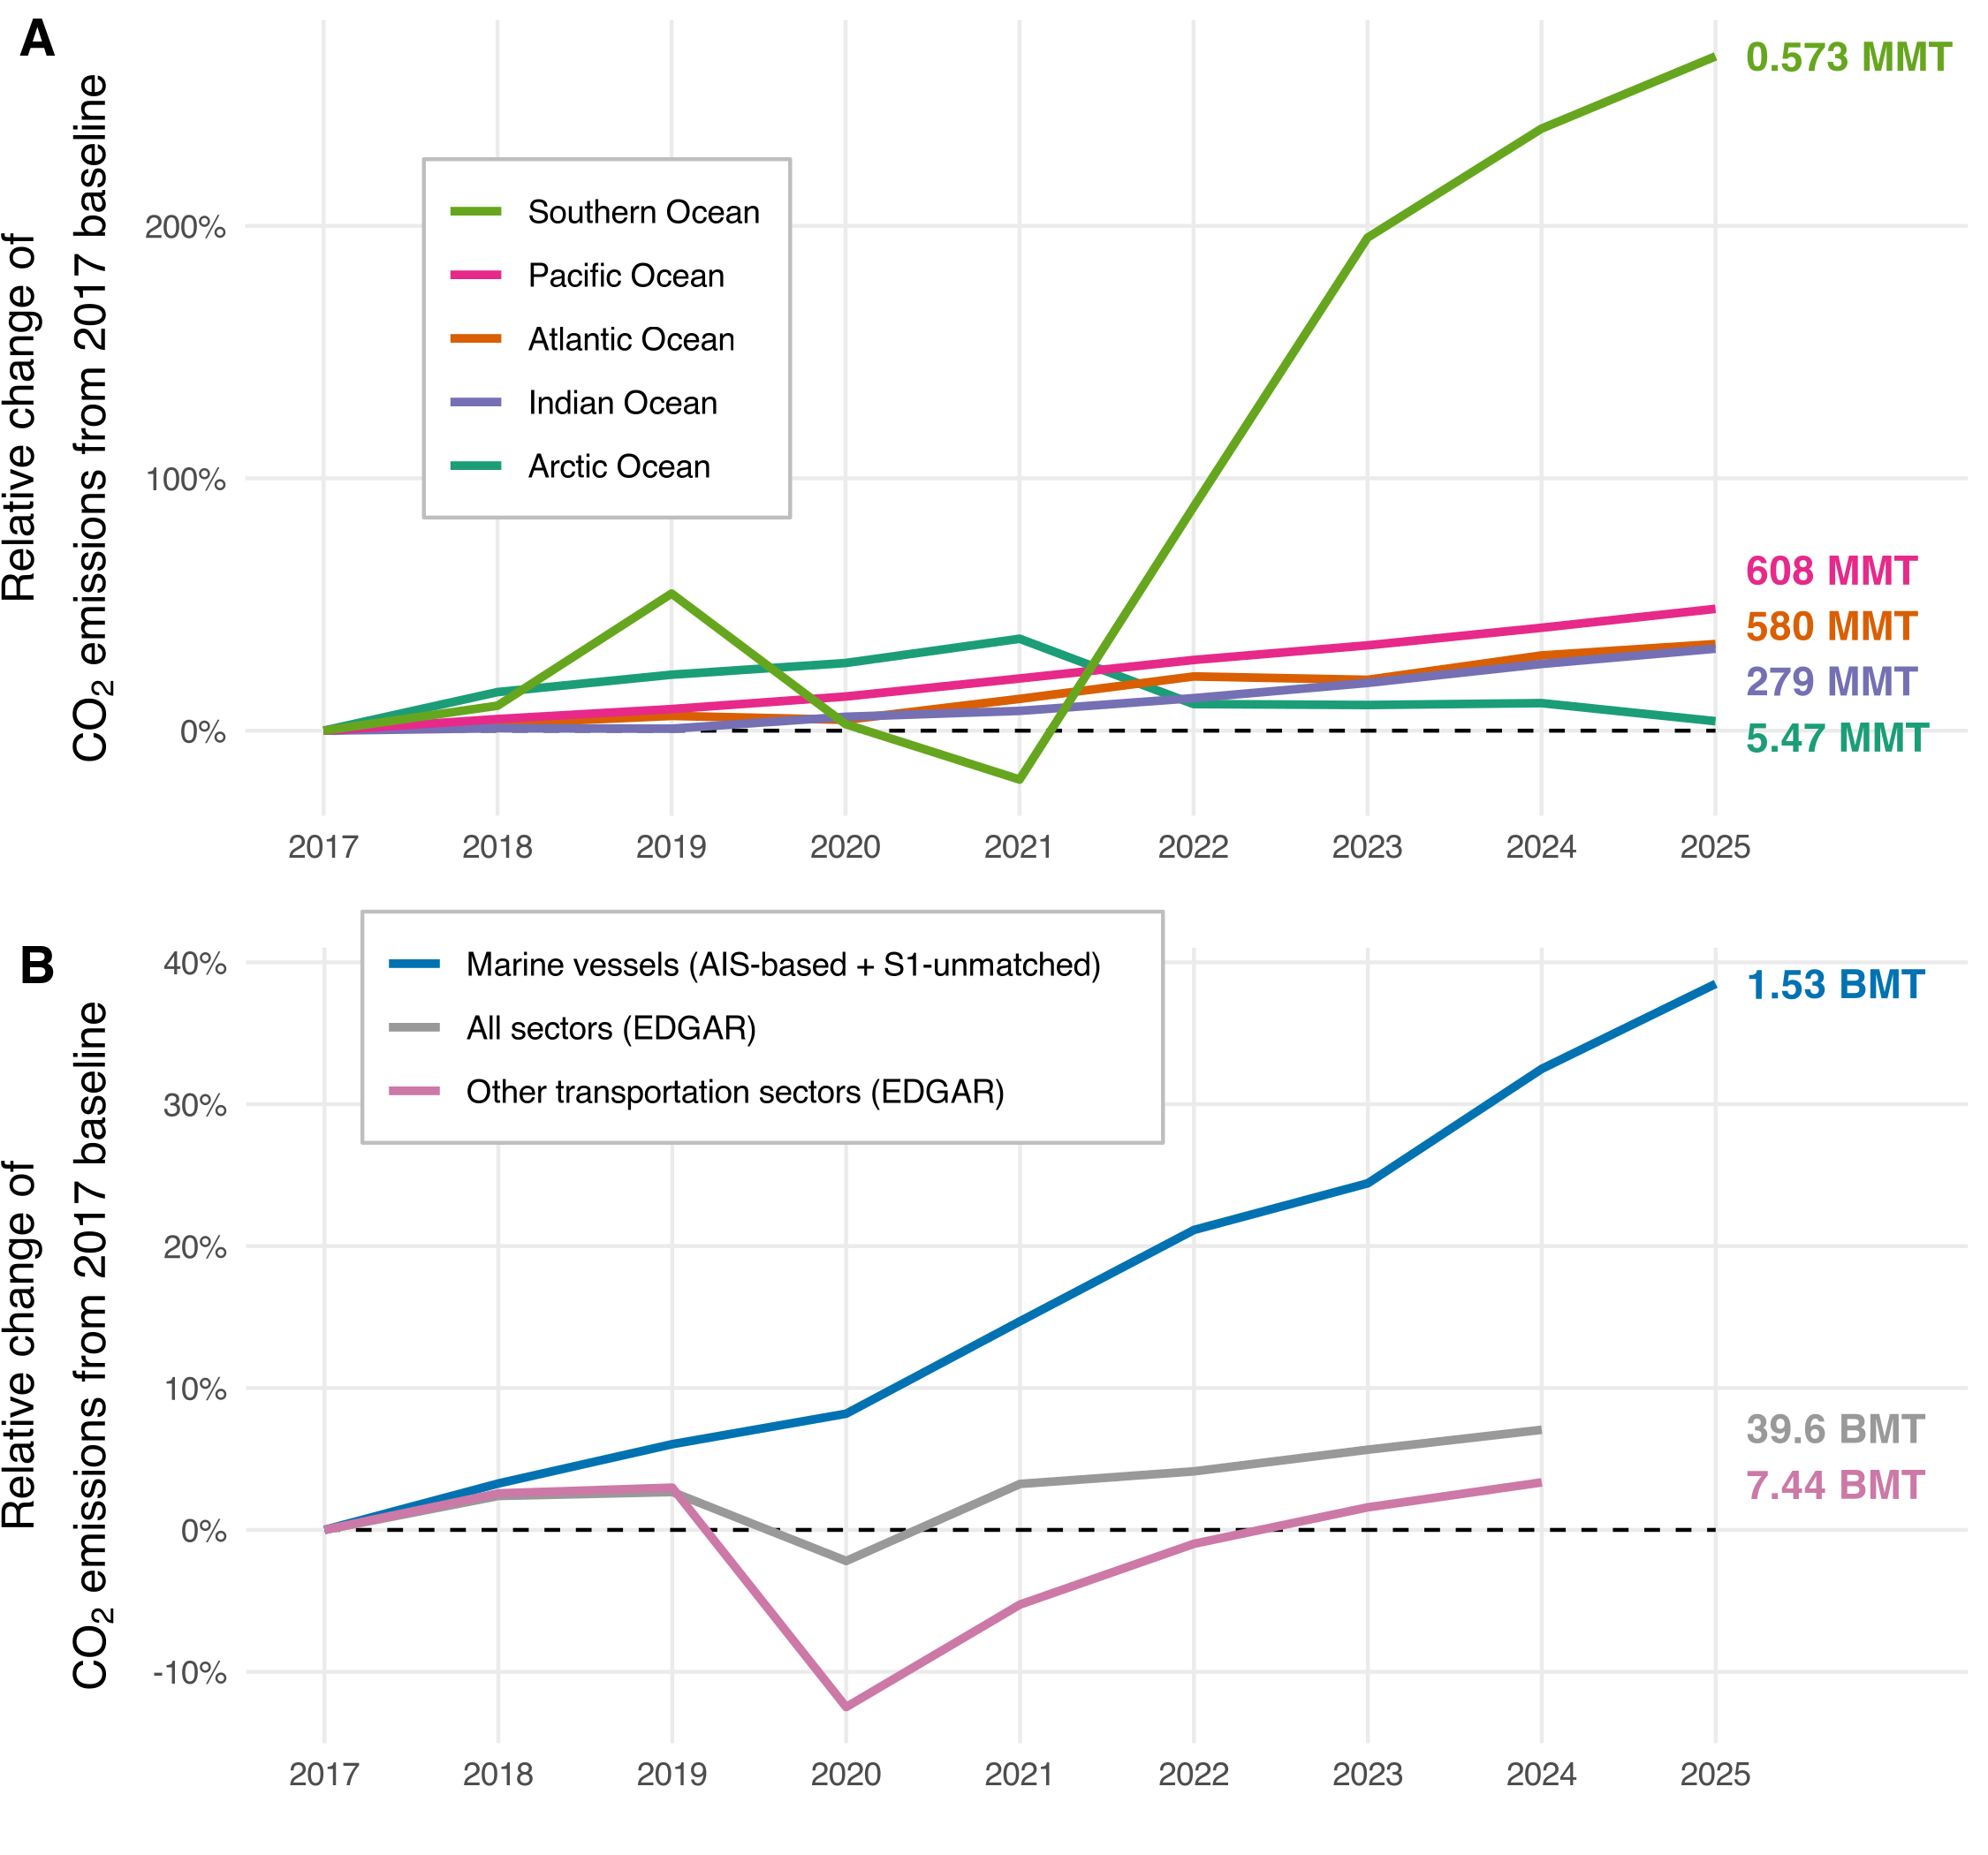
\includegraphics[width=\columnwidth]{figures/fig-emissions-marine-ocean-other-1.png}
    \caption{Trend in CO$_{2}$ emissions by ocean (normalized to 2017 baseline), using our fused AIS+S1 marine vessel data. On the right-hand side of the figure, absolute values for the last year of available data (2025) are shown as text and color-coded for each line.}
    \label{fig:fig-emissions-marine-ocean-other}
\end{figure}

\begin{figure}[H]
    \centering
    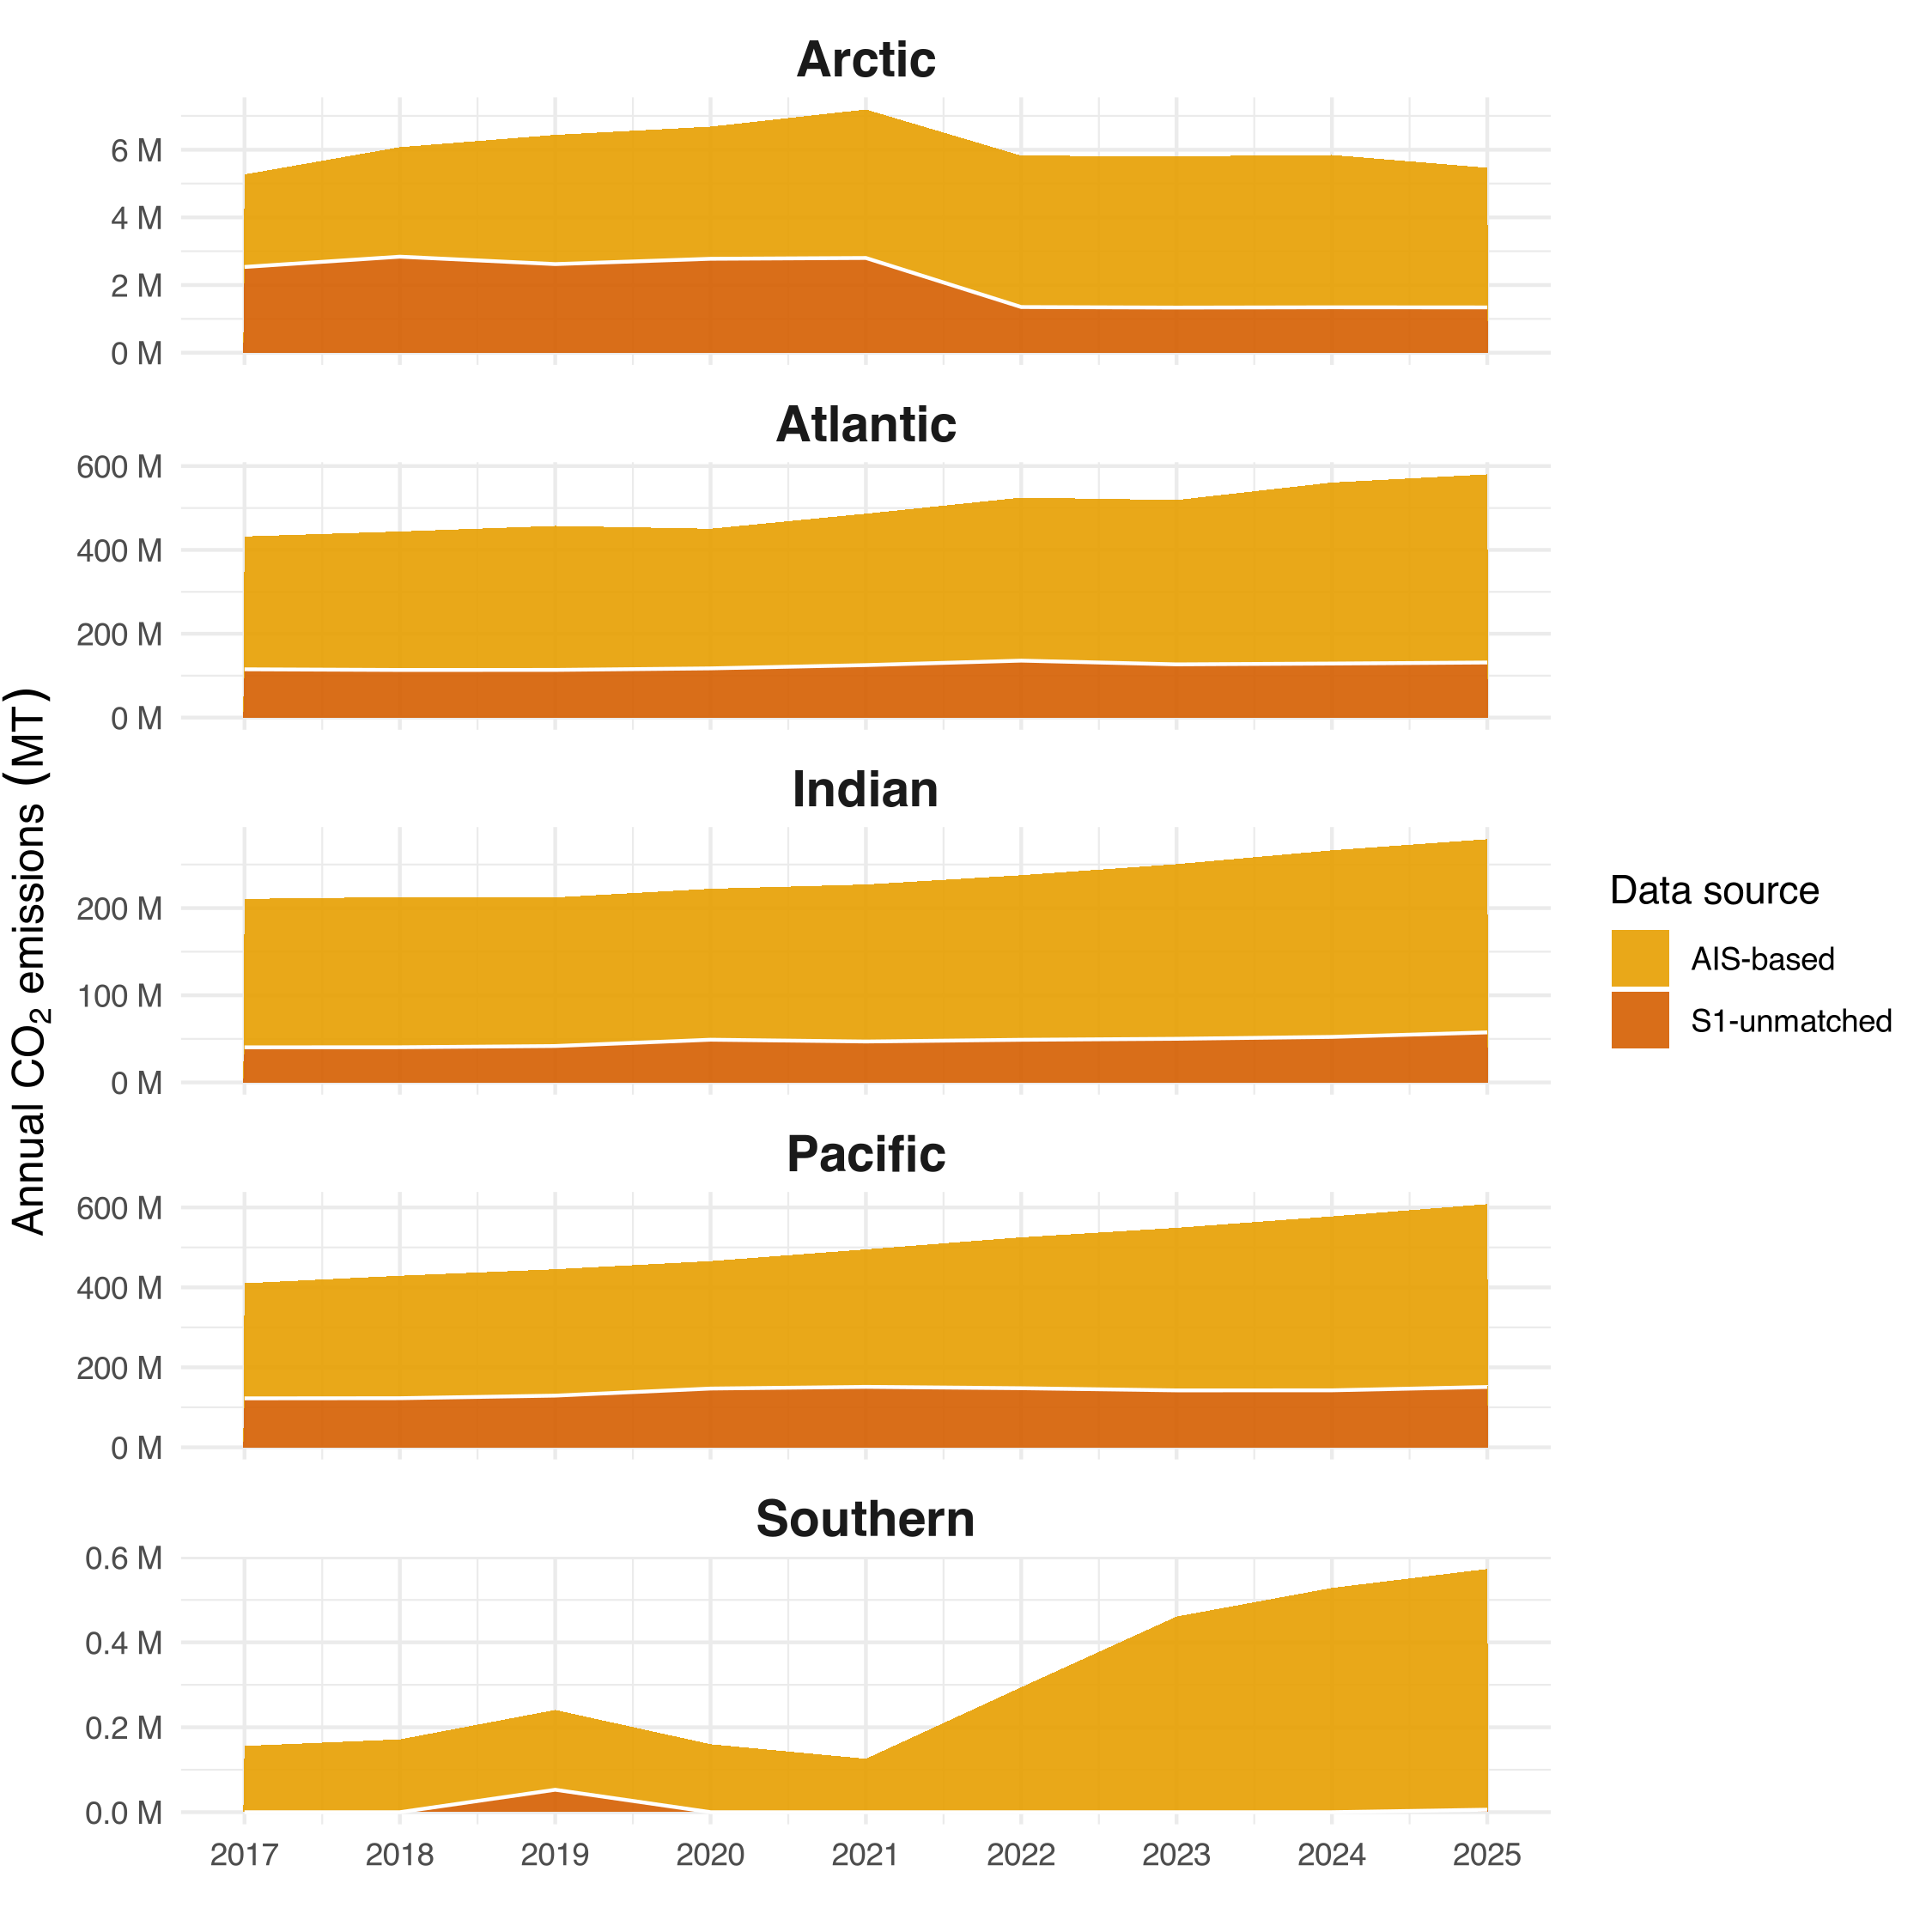
\includegraphics[width=\columnwidth]{figures/fig-annual-emissions-by-ocean-and-data-source-1.png}
    \caption{Annual total CO2 emissions by ocean, disaggregated by data source (AIS-based and S1-unmatched).}
    \label{fig:fig-annual-emissions-by-ocean-and-data-source}
\end{figure}

\begin{figure}[!p]
    \centering
    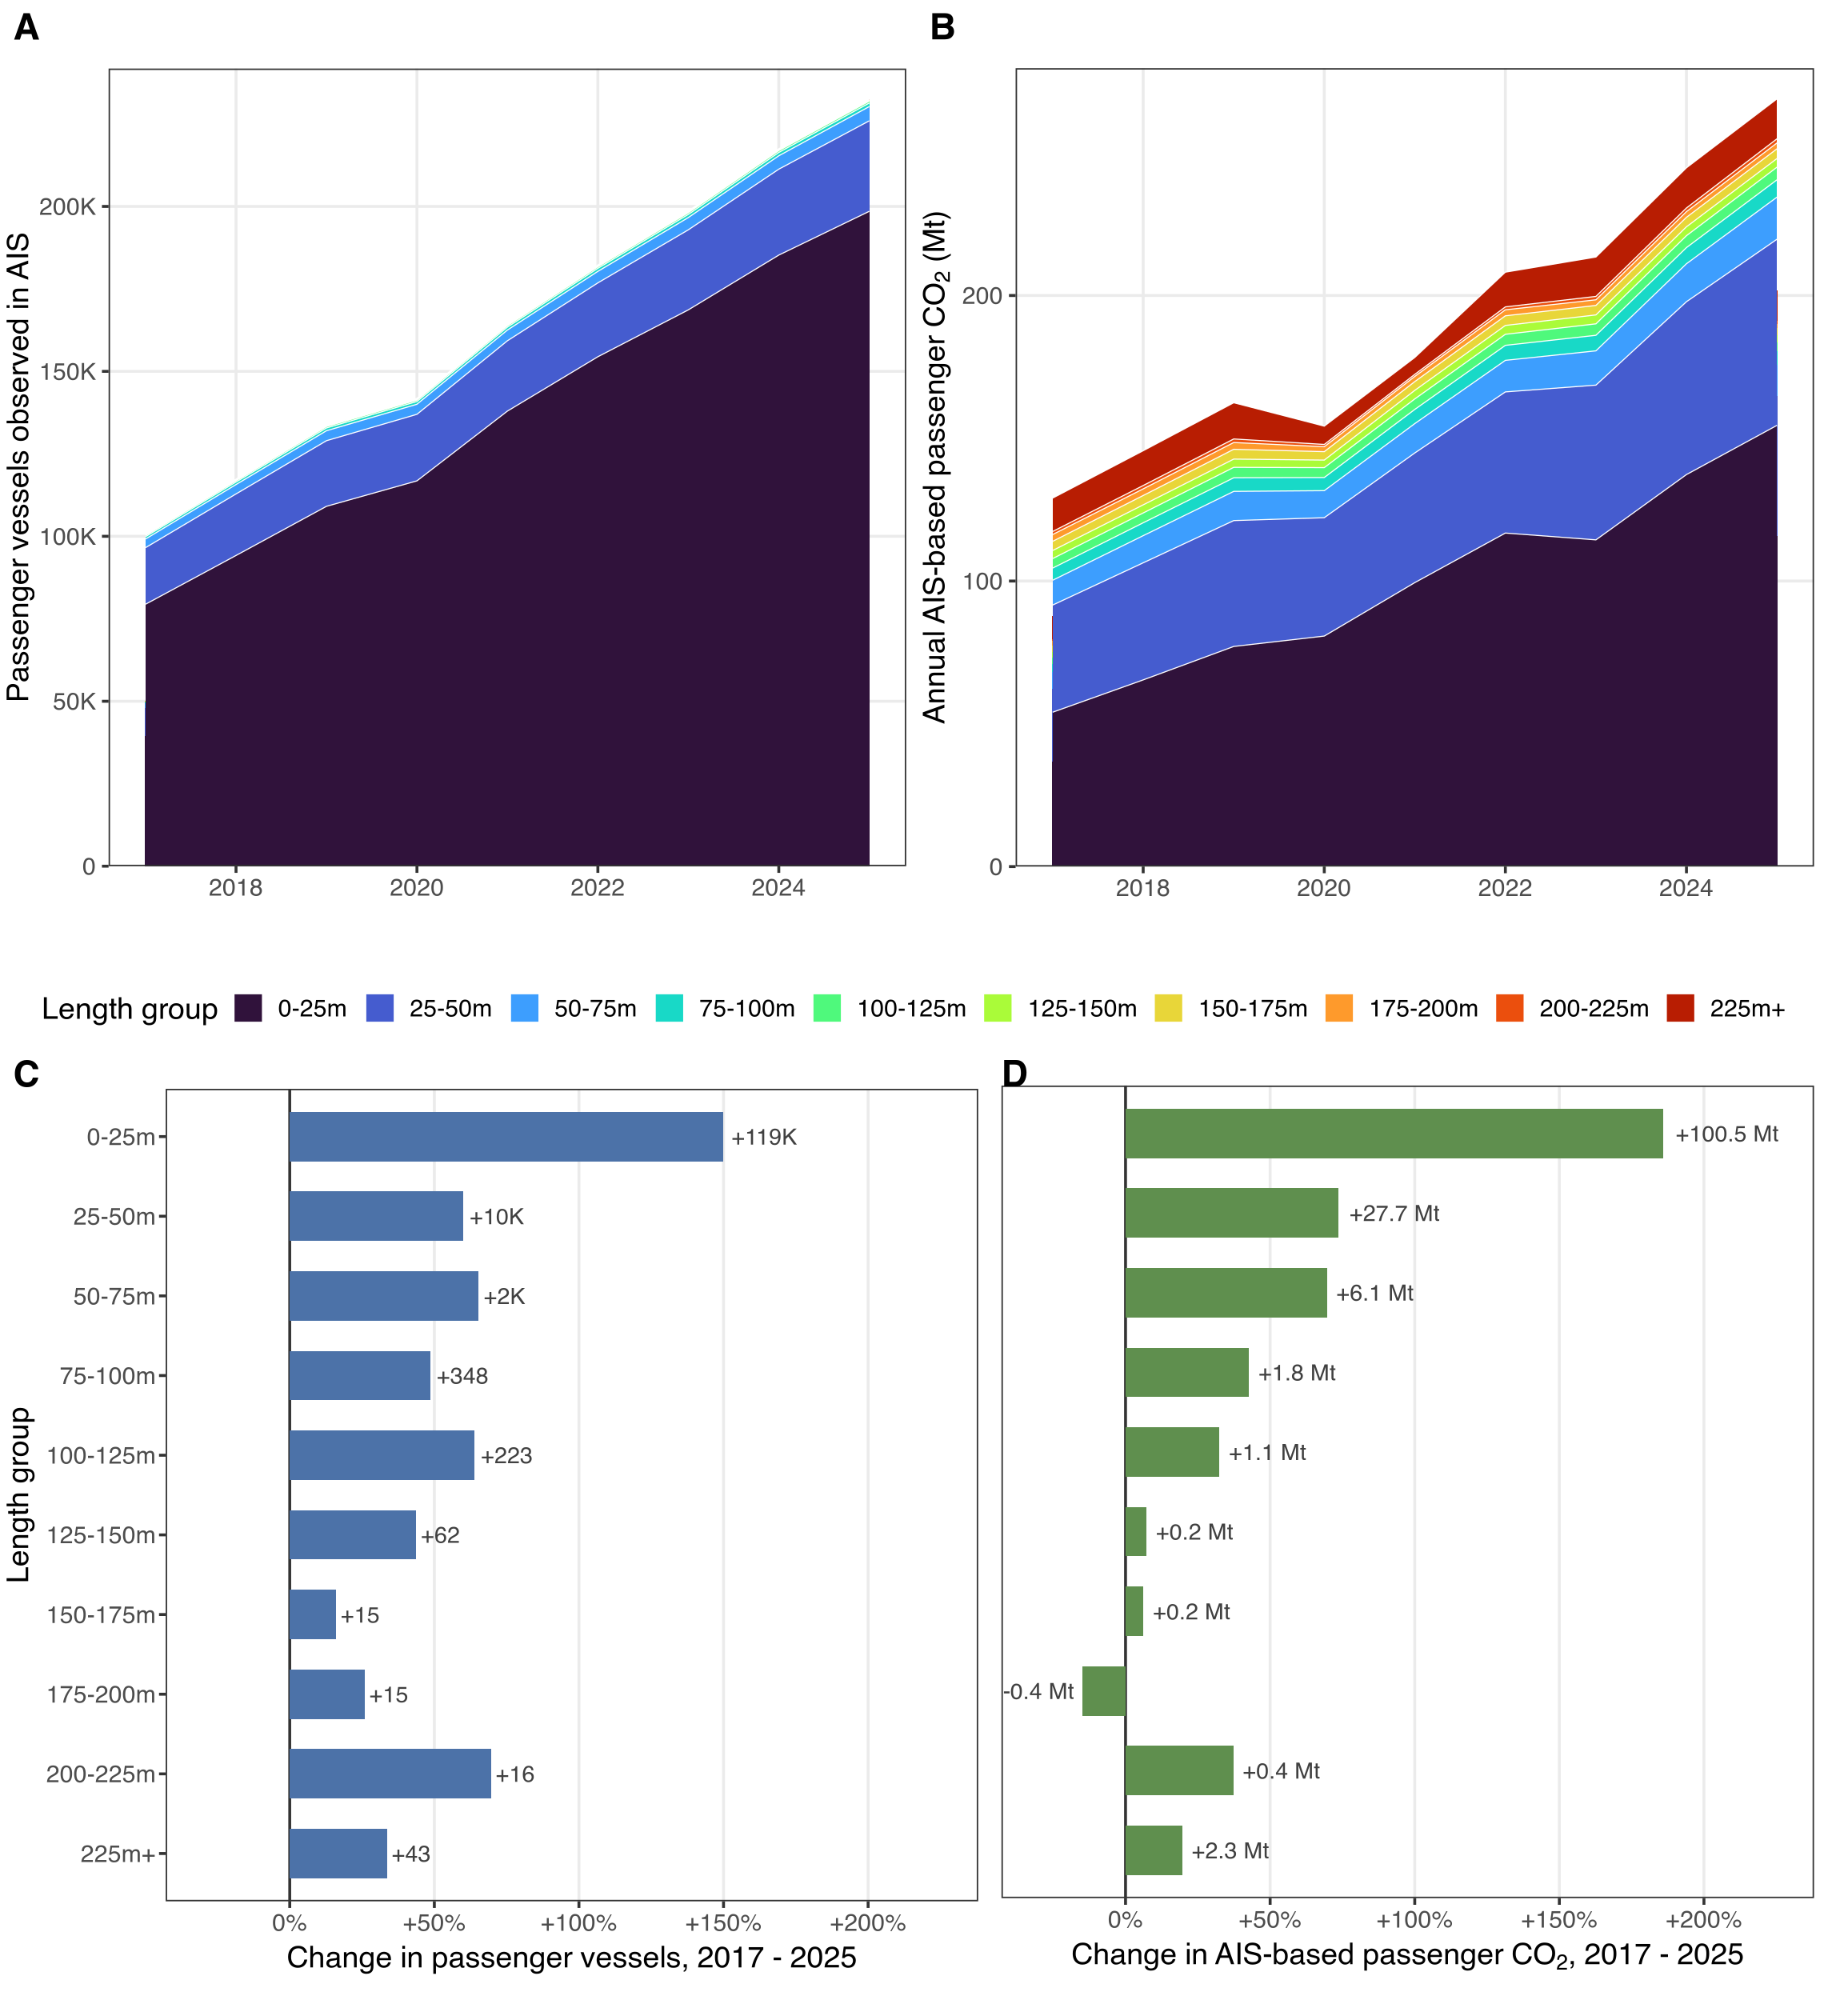
\includegraphics[width=\columnwidth,height=0.92\textheight,keepaspectratio]{figures/figS-passenger-size-panels-1.png}
    \caption{Passenger vessels by length bin, 2017 against 2025, showing growth concentrated in the smallest sizes.}
    \label{fig:figS-passenger-size-panels}
\end{figure}

\begin{figure}[H]
    \centering
    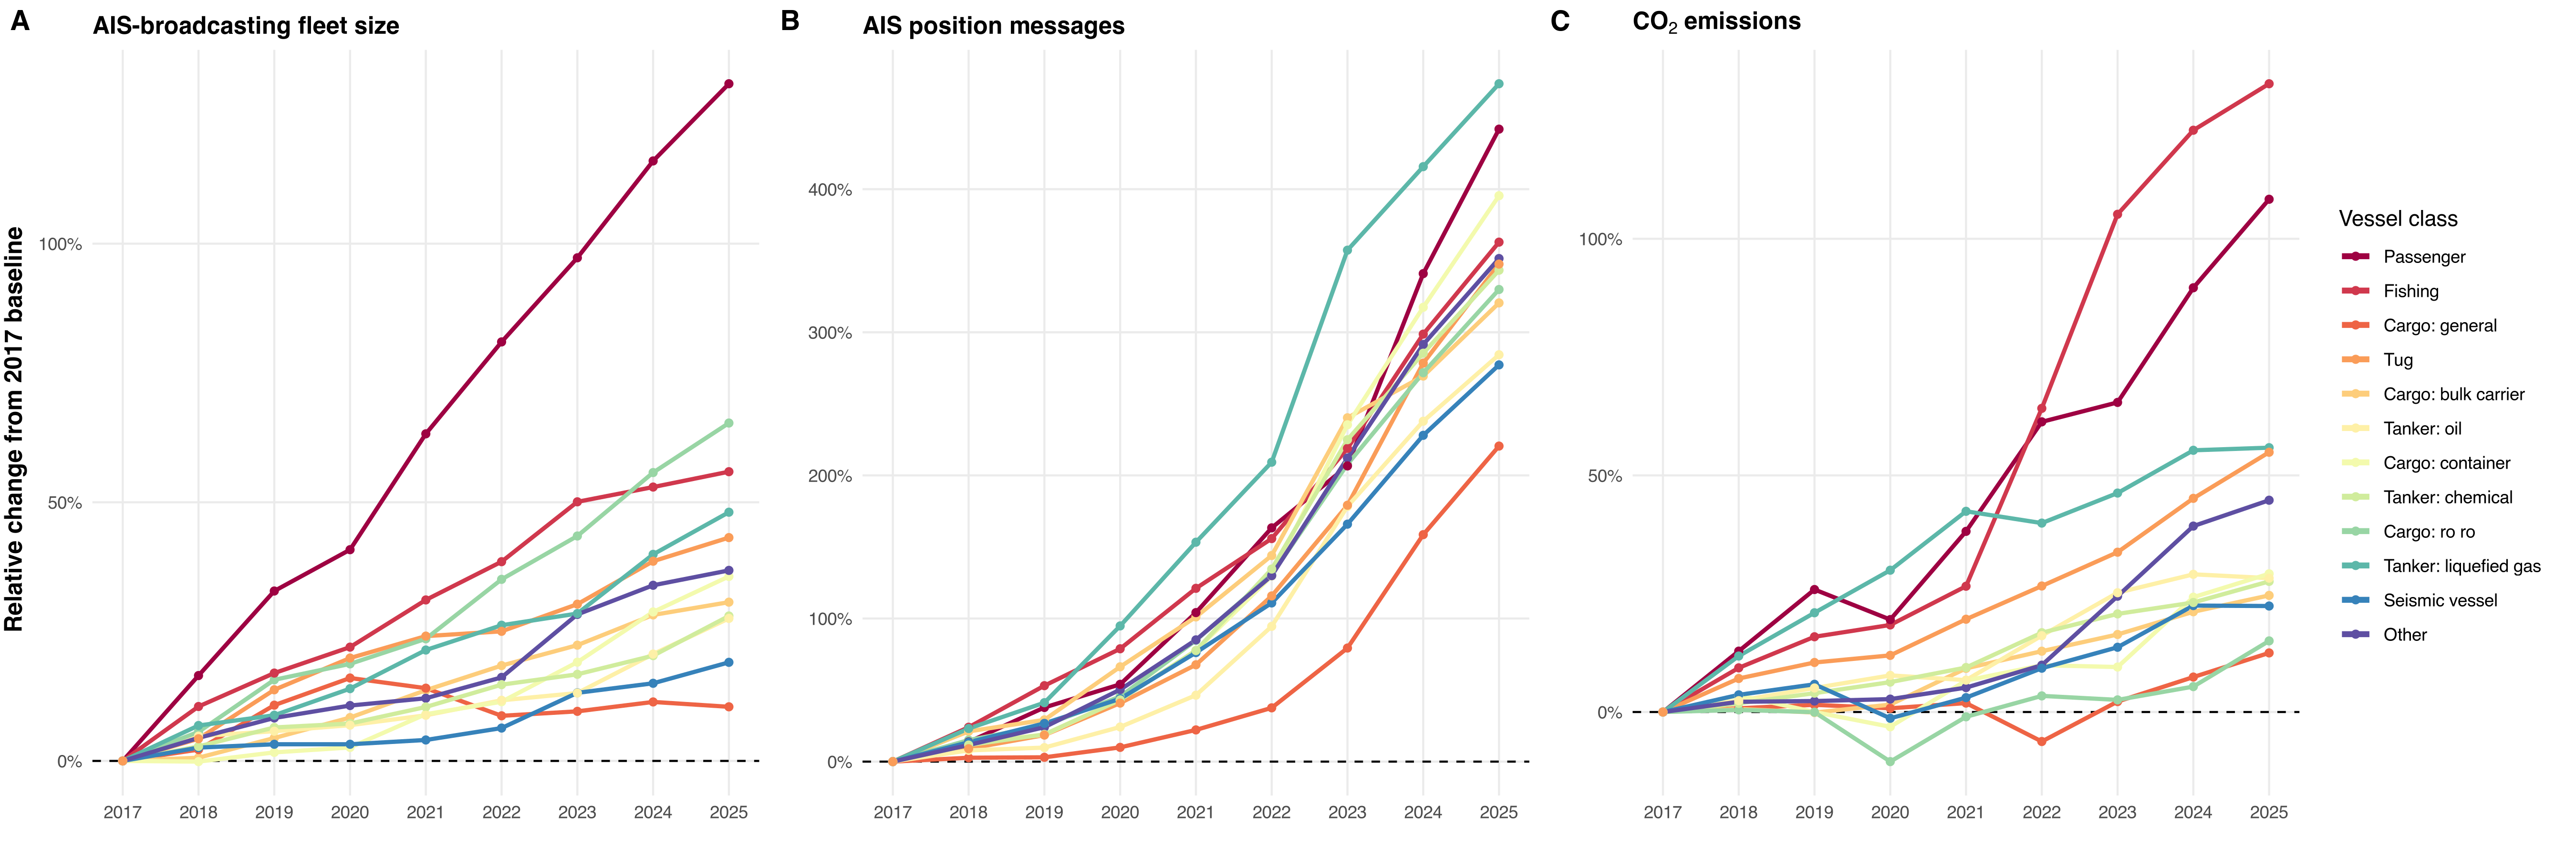
\includegraphics[width=\columnwidth]{figures/figS-fleet-growth-by-year-1.png}
    \caption{Relative change since 2017, by vessel class, in (a) the number of AIS-broadcasting vessels, (b) AIS position messages received, and (c) CO$_{2}$ emissions, for AIS-broadcasting vessels. Every panel is expressed as a change from that class's own 2017 value, so classes of very different absolute size can be read on a single scale. Growth in panels a and b reflects both genuine expansion of the fleet and its activity, and the increasing uptake and reception of AIS over the period. Passenger vessels grow fastest in fleet size and fishing vessels fastest in emissions, the two classes that other inventories are least likely to cover.}
    \label{fig:figS-fleet-growth-by-year}
\end{figure}

\begin{figure}[H]
    \centering
    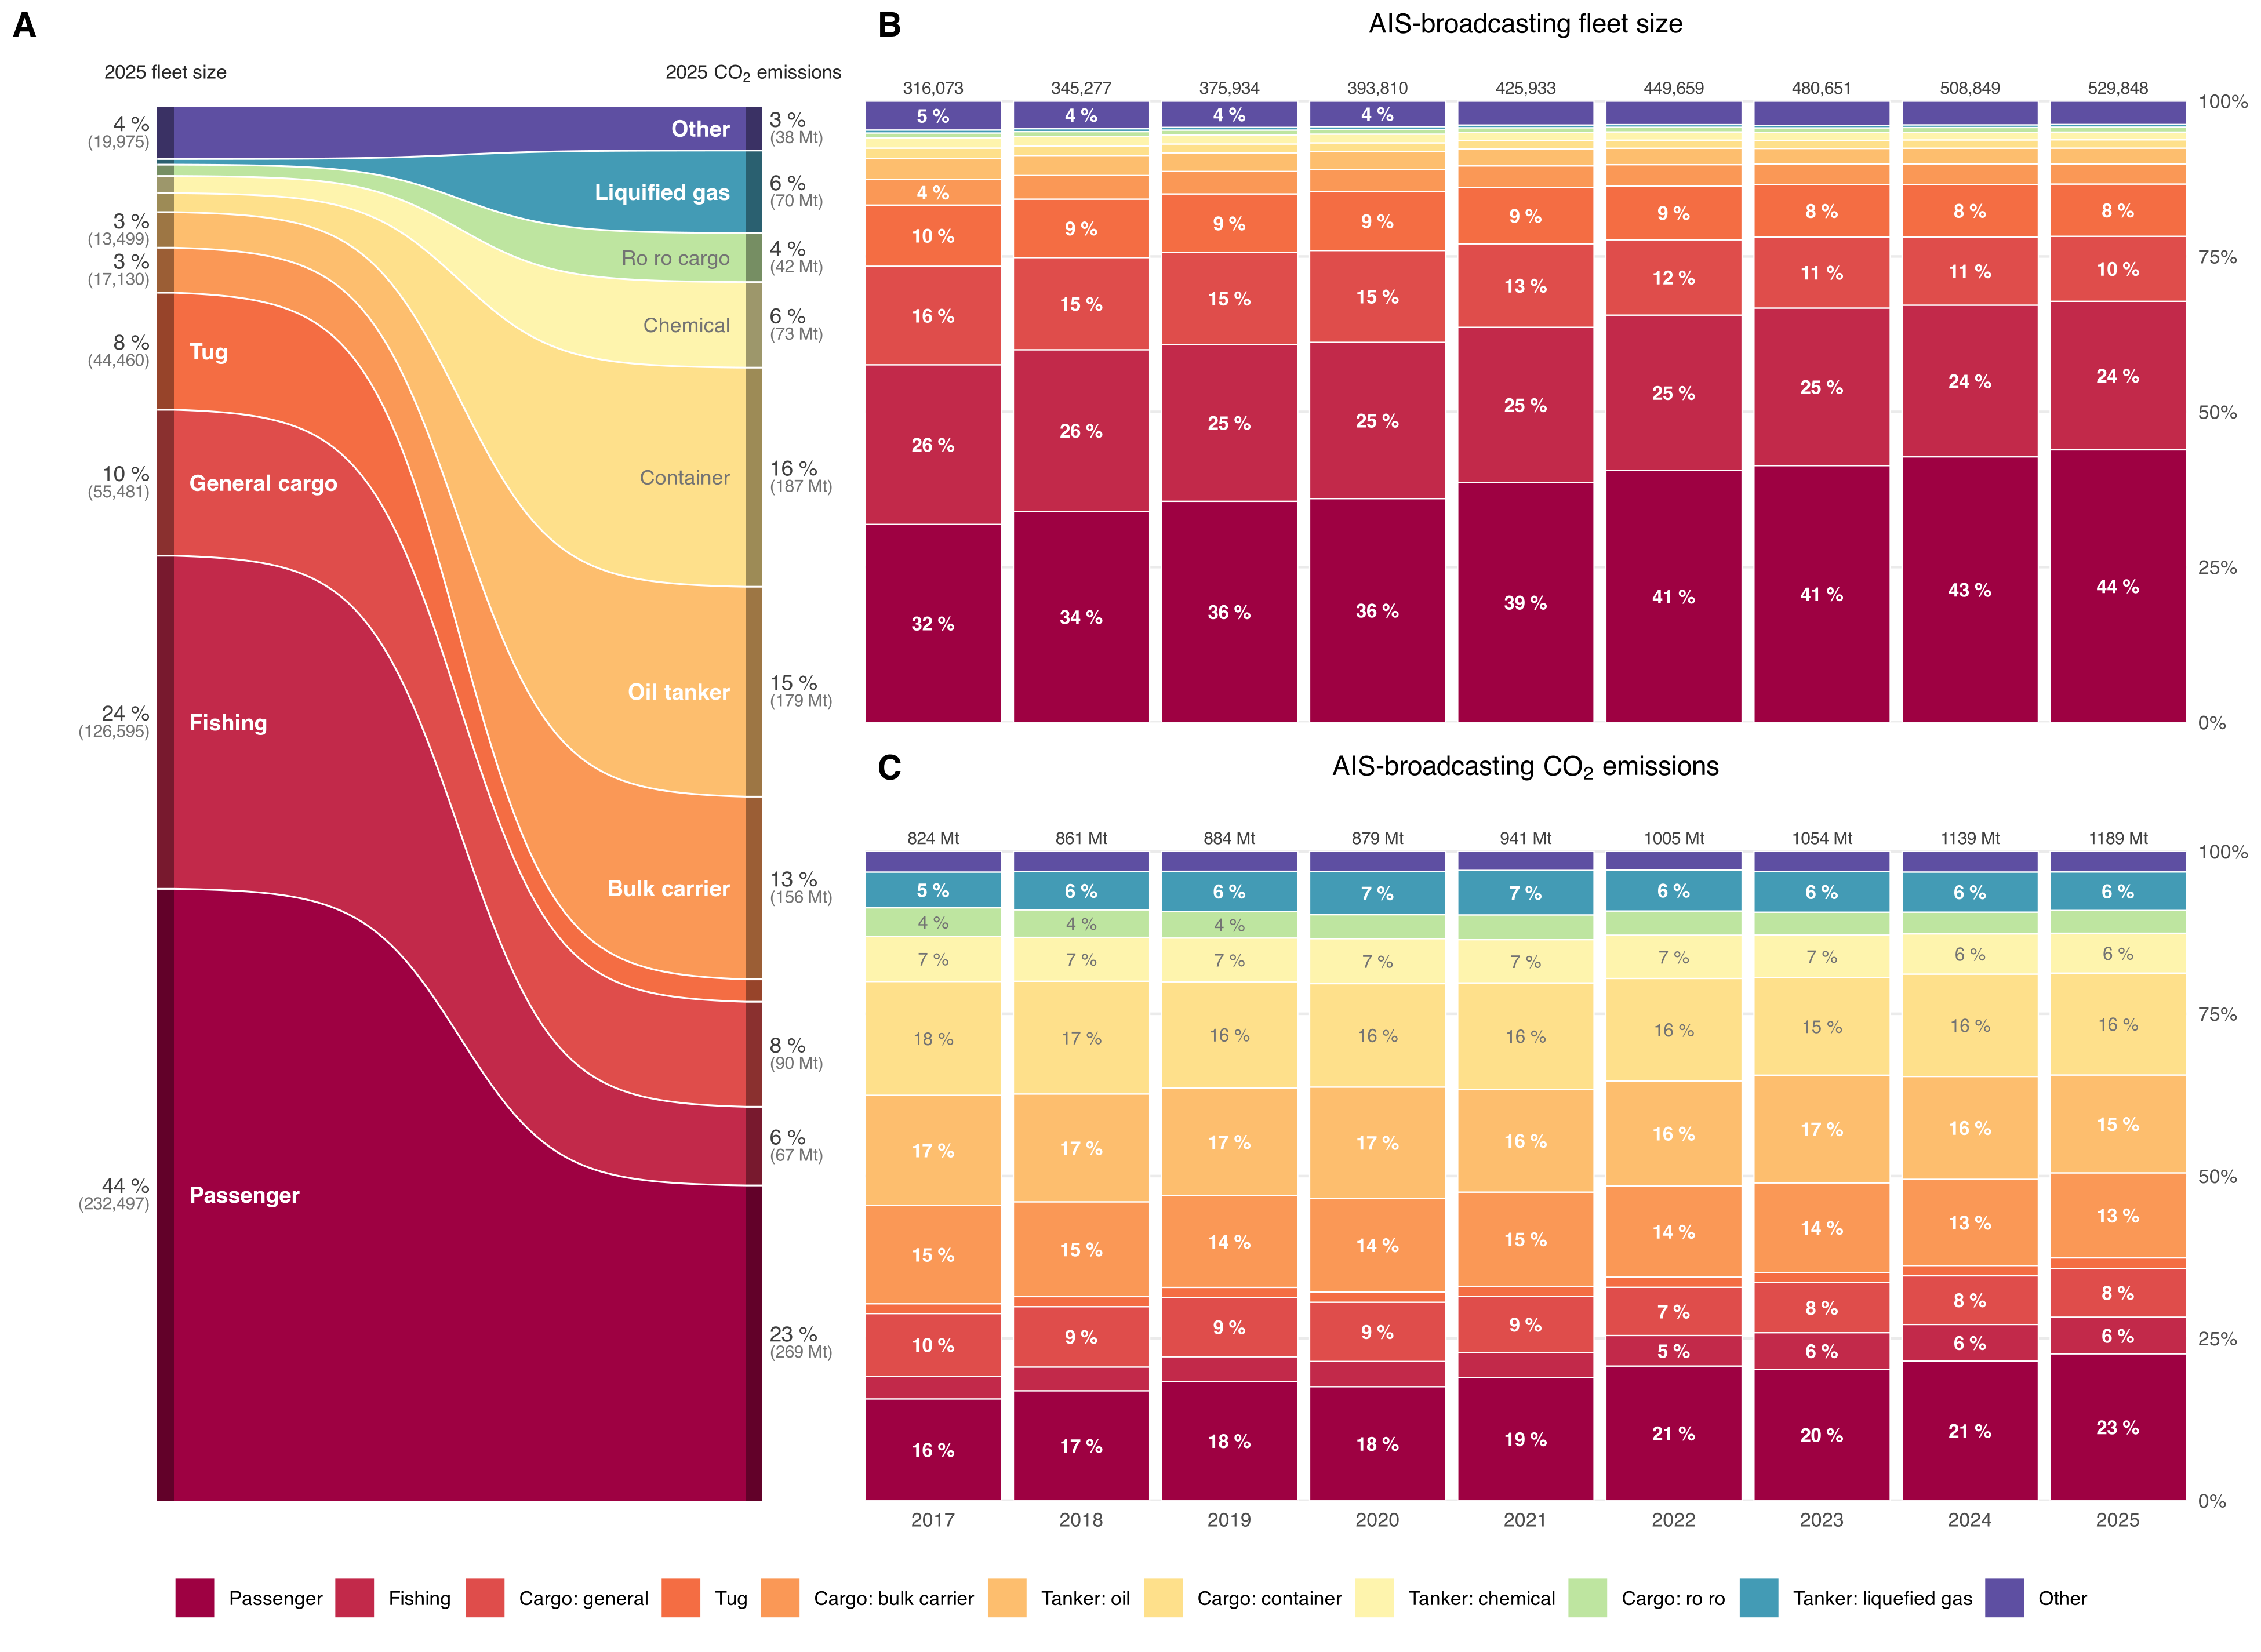
\includegraphics[width=\columnwidth]{figures/figS-fleet-sankey-with-series-2025-1.png}
    \caption{Fleet composition in 2025: each vessel class's share of the fleet against its share of CO$_{2}$, with the supporting series.}
    \label{fig:figS-fleet-sankey-with-series-2025}
\end{figure}

\section*{Supplementary Tables}

\begin{table}[!h]
\centering
\caption{\label{tab:total_percent_change_by_fleet}Summary of 2017 and 2025 emissions, data source and pollutant.}
\centering
\fontsize{6}{8}\selectfont
\setlength{\tabcolsep}{3pt}
\begin{tabular}[t]{l|l|l|l|l|l}
\hline
Source & Pollutant & \shortstack{2017\\emissions, MT} & \shortstack{2025\\emissions, MT} & \shortstack{Percent 2025\\total} & \shortstack{2017 to 2025\\change}\\
\hline
AIS-based & CO2 & 8.24e+08 & 1.19e+09 & 82\% & 44\%\\
\hline
S1-unmatched & CO2 & 2.41e+08 & 2.54e+08 & 18\% & 5\%\\
\hline
AIS-based + S1-unmatched & CO2 & 1.07e+09 & 1.44e+09 & 100\% & 35\%\\
\hline
AIS-based & CH4 & 11,500 & 15,800 & 84\% & 37\%\\
\hline
S1-unmatched & CH4 & 2,890 & 2,960 & 16\% & 3\%\\
\hline
AIS-based + S1-unmatched & CH4 & 14,400 & 18,700 & 100\% & 30\%\\
\hline
AIS-based & N2O & 41,800 & 59,500 & 83\% & 42\%\\
\hline
S1-unmatched & N2O & 11,800 & 12,400 & 17\% & 5\%\\
\hline
AIS-based + S1-unmatched & N2O & 53,600 & 71,900 & 100\% & 34\%\\
\hline
AIS-based & CO & 628,000 & 865,000 & 84\% & 38\%\\
\hline
S1-unmatched & CO & 160,000 & 165,000 & 16\% & 3\%\\
\hline
AIS-based + S1-unmatched & CO & 788,000 & 1,030,000 & 100\% & 31\%\\
\hline
AIS-based & NOX & 14,100,000 & 18,500,000 & 85\% & 31\%\\
\hline
S1-unmatched & NOX & 3,320,000 & 3,320,000 & 15\% & 0\%\\
\hline
AIS-based + S1-unmatched & NOX & 17,400,000 & 21,800,000 & 100\% & 25\%\\
\hline
AIS-based & SOX & 5,030,000 & 1,830,000 & 82\% & -64\%\\
\hline
S1-unmatched & SOX & 1,490,000 & 390,000 & 18\% & -74\%\\
\hline
AIS-based + S1-unmatched & SOX & 6,520,000 & 2,220,000 & 100\% & -66\%\\
\hline
AIS-based & PM2.5 & 701,000 & 590,000 & 84\% & -16\%\\
\hline
S1-unmatched & PM2.5 & 192,000 & 113,000 & 16\% & -41\%\\
\hline
AIS-based + S1-unmatched & PM2.5 & 893,000 & 703,000 & 100\% & -21\%\\
\hline
AIS-based & PM10 & 762,000 & 641,000 & 84\% & -16\%\\
\hline
S1-unmatched & PM10 & 209,000 & 123,000 & 16\% & -41\%\\
\hline
AIS-based + S1-unmatched & PM10 & 971,000 & 764,000 & 100\% & -21\%\\
\hline
AIS-based & VOCs & 641,000 & 868,000 & 85\% & 35\%\\
\hline
S1-unmatched & VOCs & 154,000 & 157,000 & 15\% & 2\%\\
\hline
AIS-based + S1-unmatched & VOCs & 795,000 & 1,020,000 & 100\% & 29\%\\
\hline
\end{tabular}
\end{table}

\FloatBarrier

\begin{table}[!h]
\centering
\caption{\label{tab:pollutant_ais_underestimation_overestimation_summary}Underestimation of 2025 emissions using only AIS data, and overestimation of 2017 to 2025 emissions trend using only AIS data, by pollutant.}
\centering
\fontsize{8}{10}\selectfont
\begin{tabular}[t]{l|l|l}
\hline
Pollutant & Underestimation of 2025 emissions & Overestimation of 2017-2025 emissions trend\\
\hline
CO2 & 18\% & 25\%\\
\hline
CH4 & 16\% & 23\%\\
\hline
N2O & 17\% & 24\%\\
\hline
CO & 16\% & 23\%\\
\hline
NOX & 15\% & 24\%\\
\hline
SOX & 18\% & -4\%\\
\hline
PM2.5 & 16\% & -25\%\\
\hline
PM10 & 16\% & -25\%\\
\hline
VOCs & 15\% & 23\%\\
\hline
\end{tabular}
\end{table}

\FloatBarrier

\begin{table}[!h]
\centering
\caption{\label{tab:emissions_by_ocean_summary_tbl}For each ocean, summary of: 2025 total (AIS+S1) CO$_2$ emissions (metric tonnes); percentage of global total (AIS+S1) 2025 CO$_2$ emissions from across all oceans; percent of 2025 total (AIS+S1) CO$_2$ emissions that are S1-unmatched; percent change in total (AIS+S1) CO$_2$ emissions from 2017 to 2025; and the percentage of all observations in the dataset (pixel-months) from 2017-2025 that were imaged by S1.}
\centering
\begin{tabular}[t]{l|l|l|l|l|l}
\hline
Summary statistic & Southern & Pacific & Indian & Arctic & Atlantic\\
\hline
2025 total CO2 emissions (million MT) & 0.567 & 457 & 222 & 4.13 & 449\\
\hline
Percent of total CO2 2025 emissions & 0.04\% & 41.11\% & 18.78\% & 0.38\% & 39.69\%\\
\hline
Percent of total CO2 emissions S1-unmatched & 0.88\% & 23.48\% & 18.85\% & 24.91\% & 22.24\%\\
\hline
Percent change in total CO2 emissions (2017 to 2025) & 266.65\% & 43.83\% & 28.52\% & 4.76\% & 32.51\%\\
\hline
Percent observations imaged by S1 (across 2017-2025) & 0.06\% & 17.74\% & 16.99\% & 13.55\% & 35.94\%\\
\hline
\end{tabular}
\end{table}

\FloatBarrier

\begin{table}[!h]
\centering
\caption{\label{tab:social_cost_summary_tbl}For both non-fishing vessels and fishing vessels, we summarize: the total emissions (metric tonnes) of each GHG gas; the social cost associated with each GHG (USD/metric tonne); the social cost of each (USD); the total social cost summed across all three gases (USD). We use 2021 for non-fishing vessels since it is the year for which we have the total value of all traded goods at sea. We use 2022 for fishing vessels since it is the year for which we have the total value of wild capture fisheries.}
\centering
\fontsize{8}{10}\selectfont
\begin{tabular}[t]{l|l|l|l|l|r}
\hline
Year & Vessel type & GHG & Emissions (MT) & SC (USD/MT) & SC (billion USD)\\
\hline
2021 & Non-fishing & CH4 & 14,397 & 2,900 & 0.042\\
\hline
2021 & Non-fishing & CO2 & 1,126,563,963 & 283 & 318.818\\
\hline
2021 & Non-fishing & N2O & 56,302 & 49,600 & 2.793\\
\hline
Total & Non-fishing & - & - & - & 321.652\\
\hline
2022 & Fishing & CH4 & 1,346 & 2,900 & 0.004\\
\hline
2022 & Fishing & CO2 & 81,011,499 & 283 & 22.926\\
\hline
2022 & Fishing & N2O & 4,127 & 49,600 & 0.205\\
\hline
Total & Fishing & - & - & - & 23.135\\
\hline
\end{tabular}
\end{table}

\FloatBarrier

\begin{table}[!h]
\centering
\caption{\label{tab:top_countries_by_activity_type}Top 30 countries by 2025 CO$_{2}$ emissions (millions of metric tonnes) from AIS-broadcasting vessels, shown separately for each activity type, with all remaining countries pooled into a single Other row. Emissions for each international trip are partitioned equally to its departure and arrival country. These are the totals mapped in Figure \ref{fig:fig-emissions-by-country-and-activity-type}.}
\centering
\resizebox{\ifdim\width>\linewidth\linewidth\else\width\fi}{!}{
\fontsize{7}{9}\selectfont
\begin{tabular}[t]{lrlrlr}
\toprule
\multicolumn{2}{c}{International trips} & \multicolumn{2}{c}{Port stays} & \multicolumn{2}{c}{Domestic trips} \\
\cmidrule(l{3pt}r{3pt}){1-2} \cmidrule(l{3pt}r{3pt}){3-4} \cmidrule(l{3pt}r{3pt}){5-6}
Country & CO$_{2}$ & Country & CO$_{2}$ & Country & CO$_{2}$\\
\midrule
China & 55.5 & China & 74.0 & China & 66.8\\
Malaysia & 48.1 & United States & 27.8 & Japan & 13.1\\
United States & 39.9 & Indonesia & 10.6 & United States & 13.1\\
South Korea & 20.2 & Spain & 9.8 & Indonesia & 8.8\\
Australia & 19.1 & South Korea & 9.0 & South Korea & 5.7\\
\addlinespace
Brazil & 18.9 & Netherlands & 9.0 & Russia & 5.6\\
Spain & 15.7 & Japan & 8.9 & Norway & 5.4\\
Japan & 15.5 & United Arab Emirates & 8.4 & Brazil & 5.2\\
India & 15.2 & Norway & 8.4 & Australia & 3.8\\
United Arab Emirates & 14.2 & Italy & 8.1 & Malaysia & 3.4\\
\addlinespace
Panama & 13.8 & Australia & 7.6 & India & 3.4\\
Singapore & 12.7 & Turkey & 7.4 & Italy & 3.2\\
Egypt & 10.4 & France & 7.2 & Spain & 3.1\\
Indonesia & 9.0 & United Kingdom & 6.7 & Turkey & 2.7\\
Russia & 8.5 & Germany & 6.0 & United Kingdom & 2.6\\
\addlinespace
United Kingdom & 7.7 & Greece & 5.8 & Canada & 2.5\\
Netherlands & 7.4 & Brazil & 5.3 & Vietnam & 2.3\\
Canada & 6.9 & Russia & 5.0 & United Arab Emirates & 2.2\\
Mexico & 6.4 & India & 4.8 & Philippines & 2.2\\
Turkey & 6.3 & Malaysia & 4.7 & Greece & 1.8\\
\addlinespace
Taiwan & 6.1 & Canada & 4.5 & Taiwan & 1.8\\
Belgium & 6.0 & Denmark & 4.4 & France & 1.7\\
France & 5.6 & Belgium & 3.9 & Egypt & 1.7\\
Saudi Arabia & 5.5 & Saudi Arabia & 3.3 & Saudi Arabia & 1.6\\
South Africa & 5.5 & Mexico & 2.8 & Mexico & 1.3\\
\addlinespace
Vietnam & 5.4 & Thailand & 2.8 & Germany & 1.1\\
Italy & 5.0 & Sweden & 2.5 & Chile & 1.1\\
Germany & 5.0 & Philippines & 2.3 & Thailand & 1.1\\
Sri Lanka & 4.9 & Taiwan & 2.2 & New Zealand & 1.0\\
Morocco & 4.7 & Egypt & 2.2 & Argentina & 1.0\\
\addlinespace
Other & 107.2 & Other & 59.3 & Other & 19.5\\
\bottomrule
\end{tabular}}
\end{table}

\FloatBarrier


\section*{Supplementary Notes}

\supnote{Trends in AIS receiver types}{sec:ais-receiver-types}

AIS messages are broadcast from vessels and then received through one of three technologies: satellite-based receivers, terrestrial receivers, and dynamic receivers. Satellite and terrestrial receivers are the oldest receiver types, while 2022 saw the widespread adoption of dynamic AIS (D-AIS) in several regions throughout the world. D-AIS is a technology that was first implemented by Spire, one of the major AIS data providers, in which satellite-enabled AIS receivers are installed on vessels that travel through some of the world's busiest shipping lanes, such as the South China Sea \cite{spire_documentation_2022}. Through GFW, we can determine the receiver type for every single AIS message in the dataset over time. In Supplementary Fig. \ref{fig:fig-annual-emissions-by-ais-receiver-type}, we summarize the amount of estimated emissions and the number of distinct vessels that were detected by the three different types of AIS receivers. In 2022, we can clearly see a sharp rise in the amount of emissions that were estimated from D-AIS, which intuitively coincides with a decrease in the emissions that are estimated from satellite and terrestrial receivers. On aggregate, this led to an increase in total estimated emissions. The number of distinct vessels detected by D-AIS also sharply rose in 2022, almost equaling the number of vessels detected by all receiver types.

\begin{figure}[H]
    \centering
    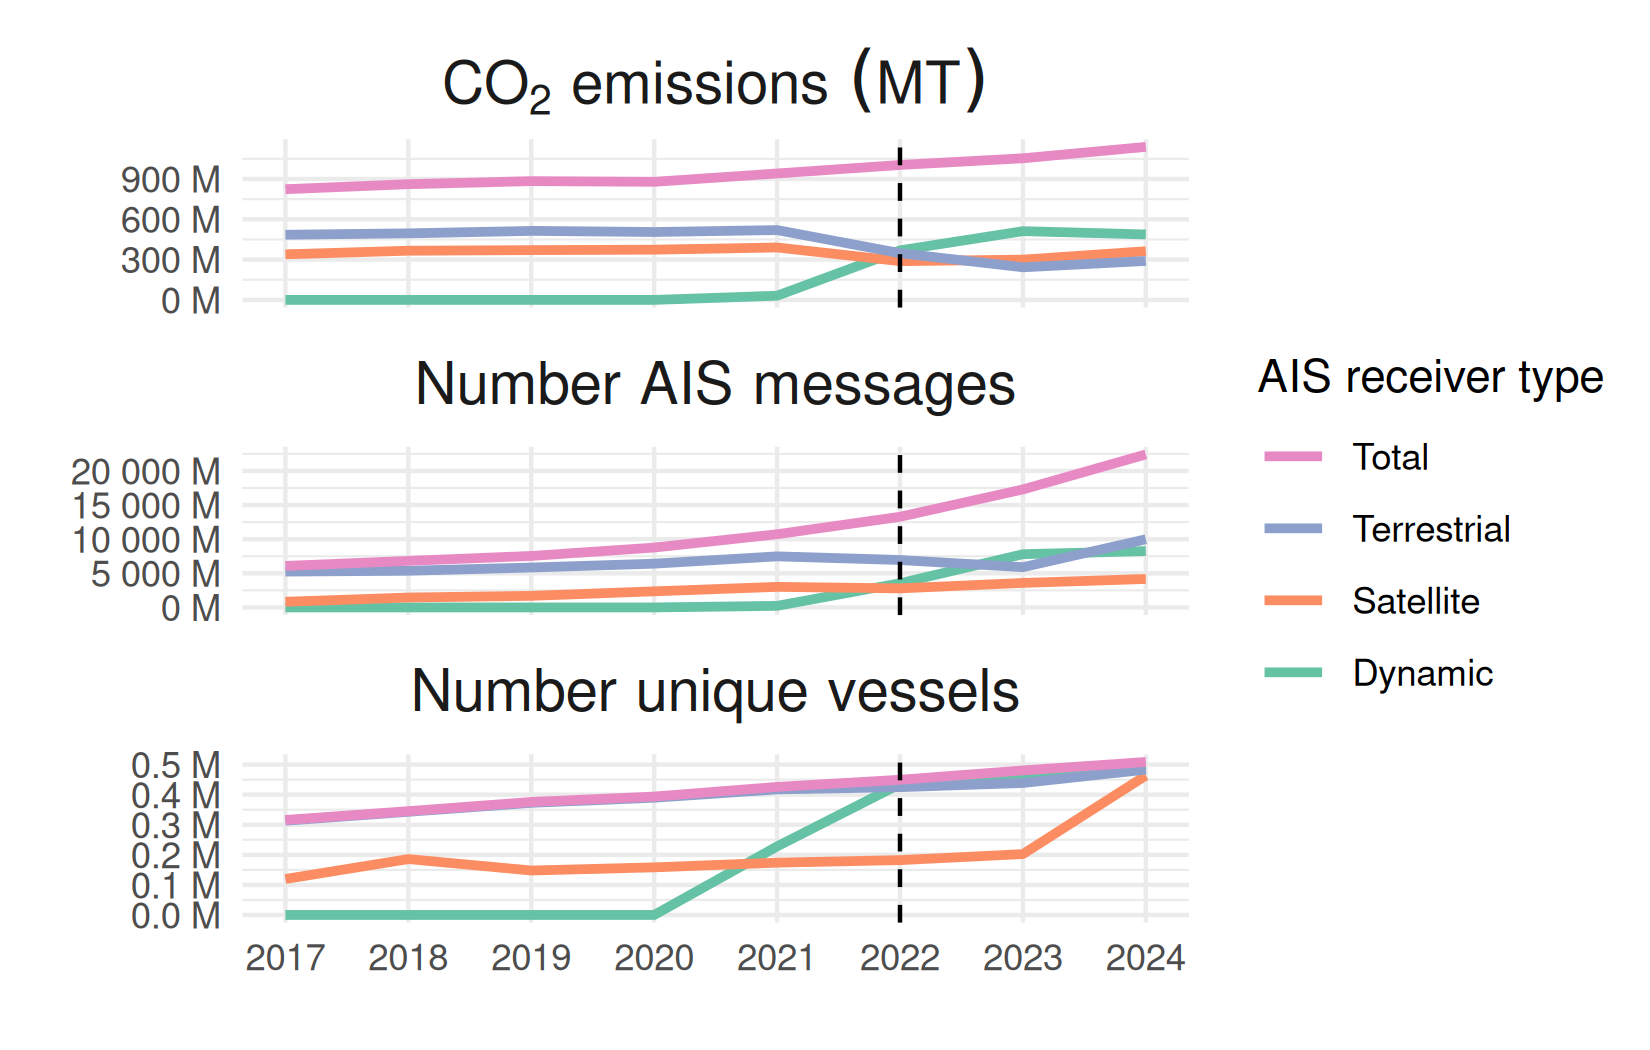
\includegraphics[width=\columnwidth]{figures/fig-annual-emissions-by-ais-receiver-type-1.png}
    \caption{Annual total CO$_{2}$ emissions (metric tonnes) by AIS-broadcasting vessels, AIS pings (i.e., individual vessel timestamped location messages), and number of unique AIS-broadcasting vessels. Trends are disaggregated by AIS receiver type (satellite, terrestrial, and dynamic), and also shown as a total aggregated across receiver types. A dashed vertical line is shown for 2022, the first year in which D-AIS was widely adopted.}
    \label{fig:fig-annual-emissions-by-ais-receiver-type}
\end{figure}

In Supplementary Fig. \ref{fig:fig-annual-emissions-by-ais-receiver-type-top-flags}, we see the amount of quantified emissions for the top 10 vessel flags broken apart by AIS receiver type. The trends are similar to those seen on aggregate ( Supplementary Fig. \ref{fig:fig-annual-emissions-by-ais-receiver-type}), although there is variation in terms of the increase in D-AIS detections across different flags. This is likely driven by whether or not each flag travels through regions where D-AIS was widely adopted. It is important to note that towards the end of 2021, China experience a blackout of terrestrial AIS signals due to new privacy laws that were being implemented \cite{benefits_dynamic_ais}.

\begin{figure}[H]
    \centering
    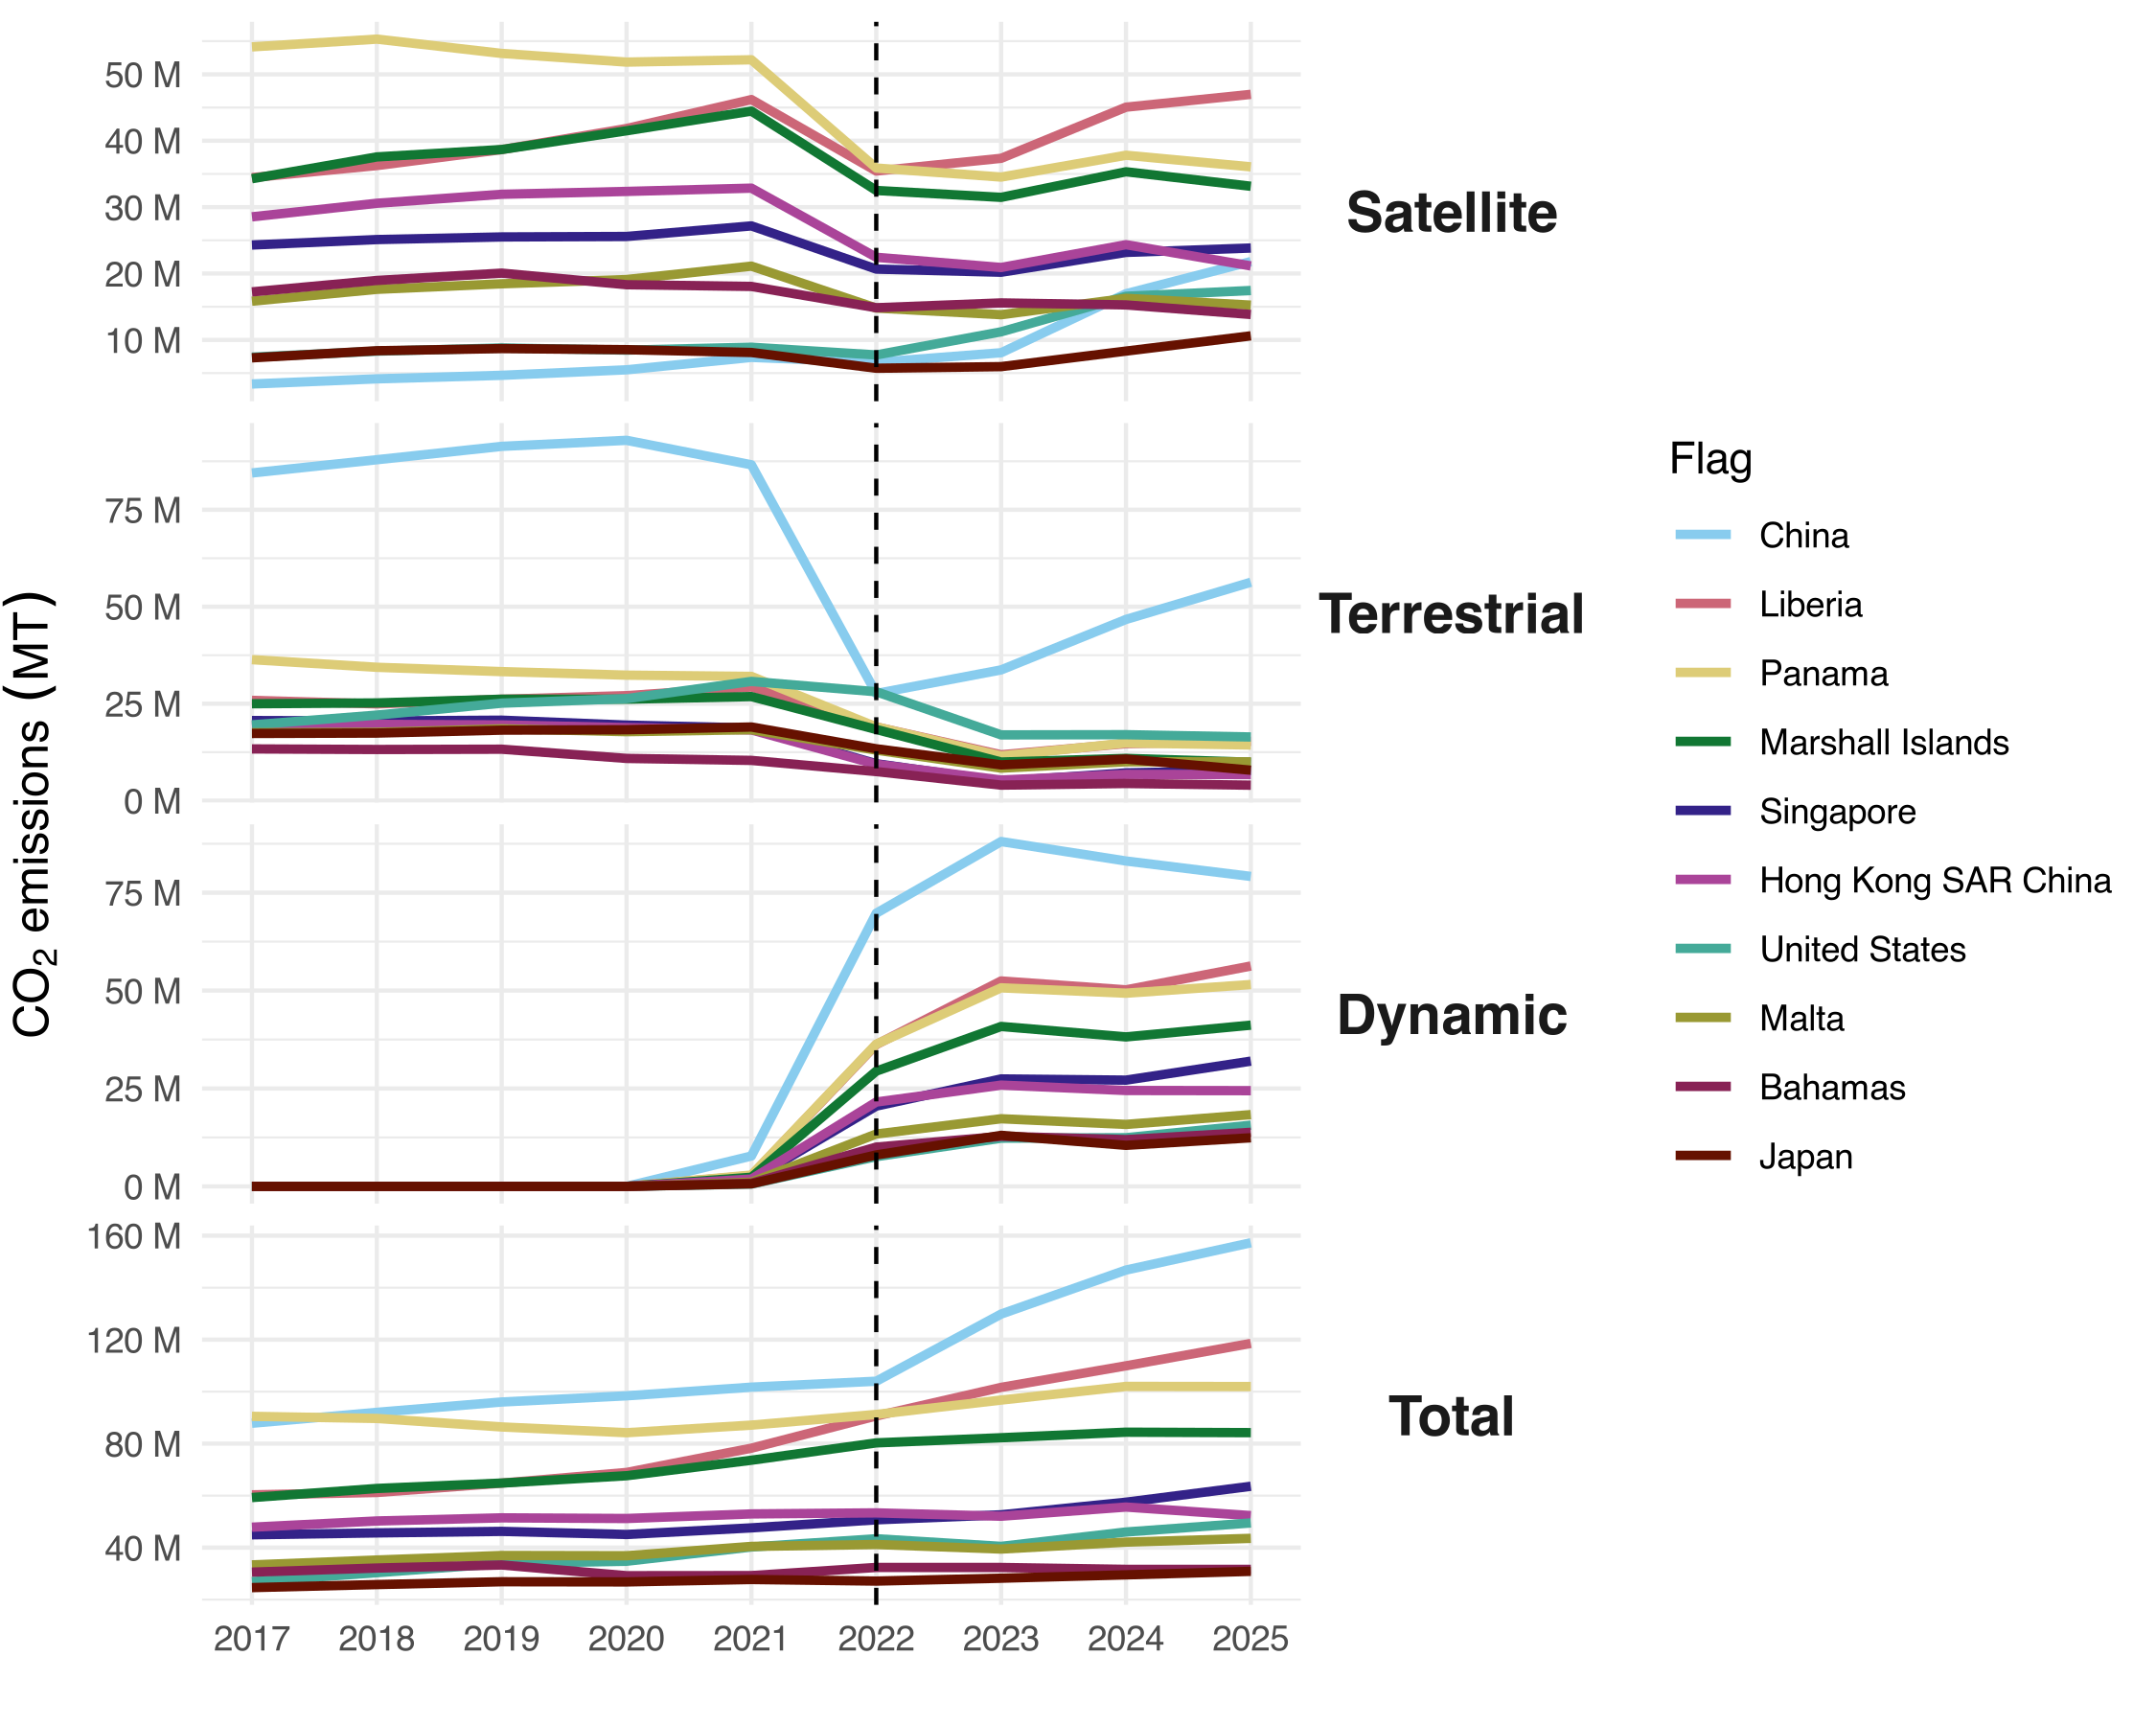
\includegraphics[width=\columnwidth]{figures/fig-annual-emissions-by-ais-receiver-type-top-flags-1.png}
    \caption{Annual total CO$_{2}$ emissions (metric tonnes) by AIS-broadcasting vessels, disaggregated by AIS receiver type (satellite, terrestrial, and dynamic) and total aggregated across receiver types, for the top 10 flags with the most emissions in 2025. A dashed vertical line is shown for 2022, the first year in which D-AIS was widely adopted.}
    \label{fig:fig-annual-emissions-by-ais-receiver-type-top-flags}
\end{figure}

Finally, in Supplementary Fig. \ref{fig:fig-co2-emissions-change-map-by-receiver-type}, we see how the use of the three AIS receiver types has changed spatially over time between 2017 and 2025. D-AIS was mostly implemented in busy shipping lanes, with clear concentration in areas including the South China Sea, Europe, and the Gulf of Mexico. These regions also generally correspond to decreasing use of satellite and terrestrial receivers. Overall, the largest total change in emissions is generally concentrated in the same regions that saw the largest uptake of D-AIS.

\begin{figure}[H]
    \centering
    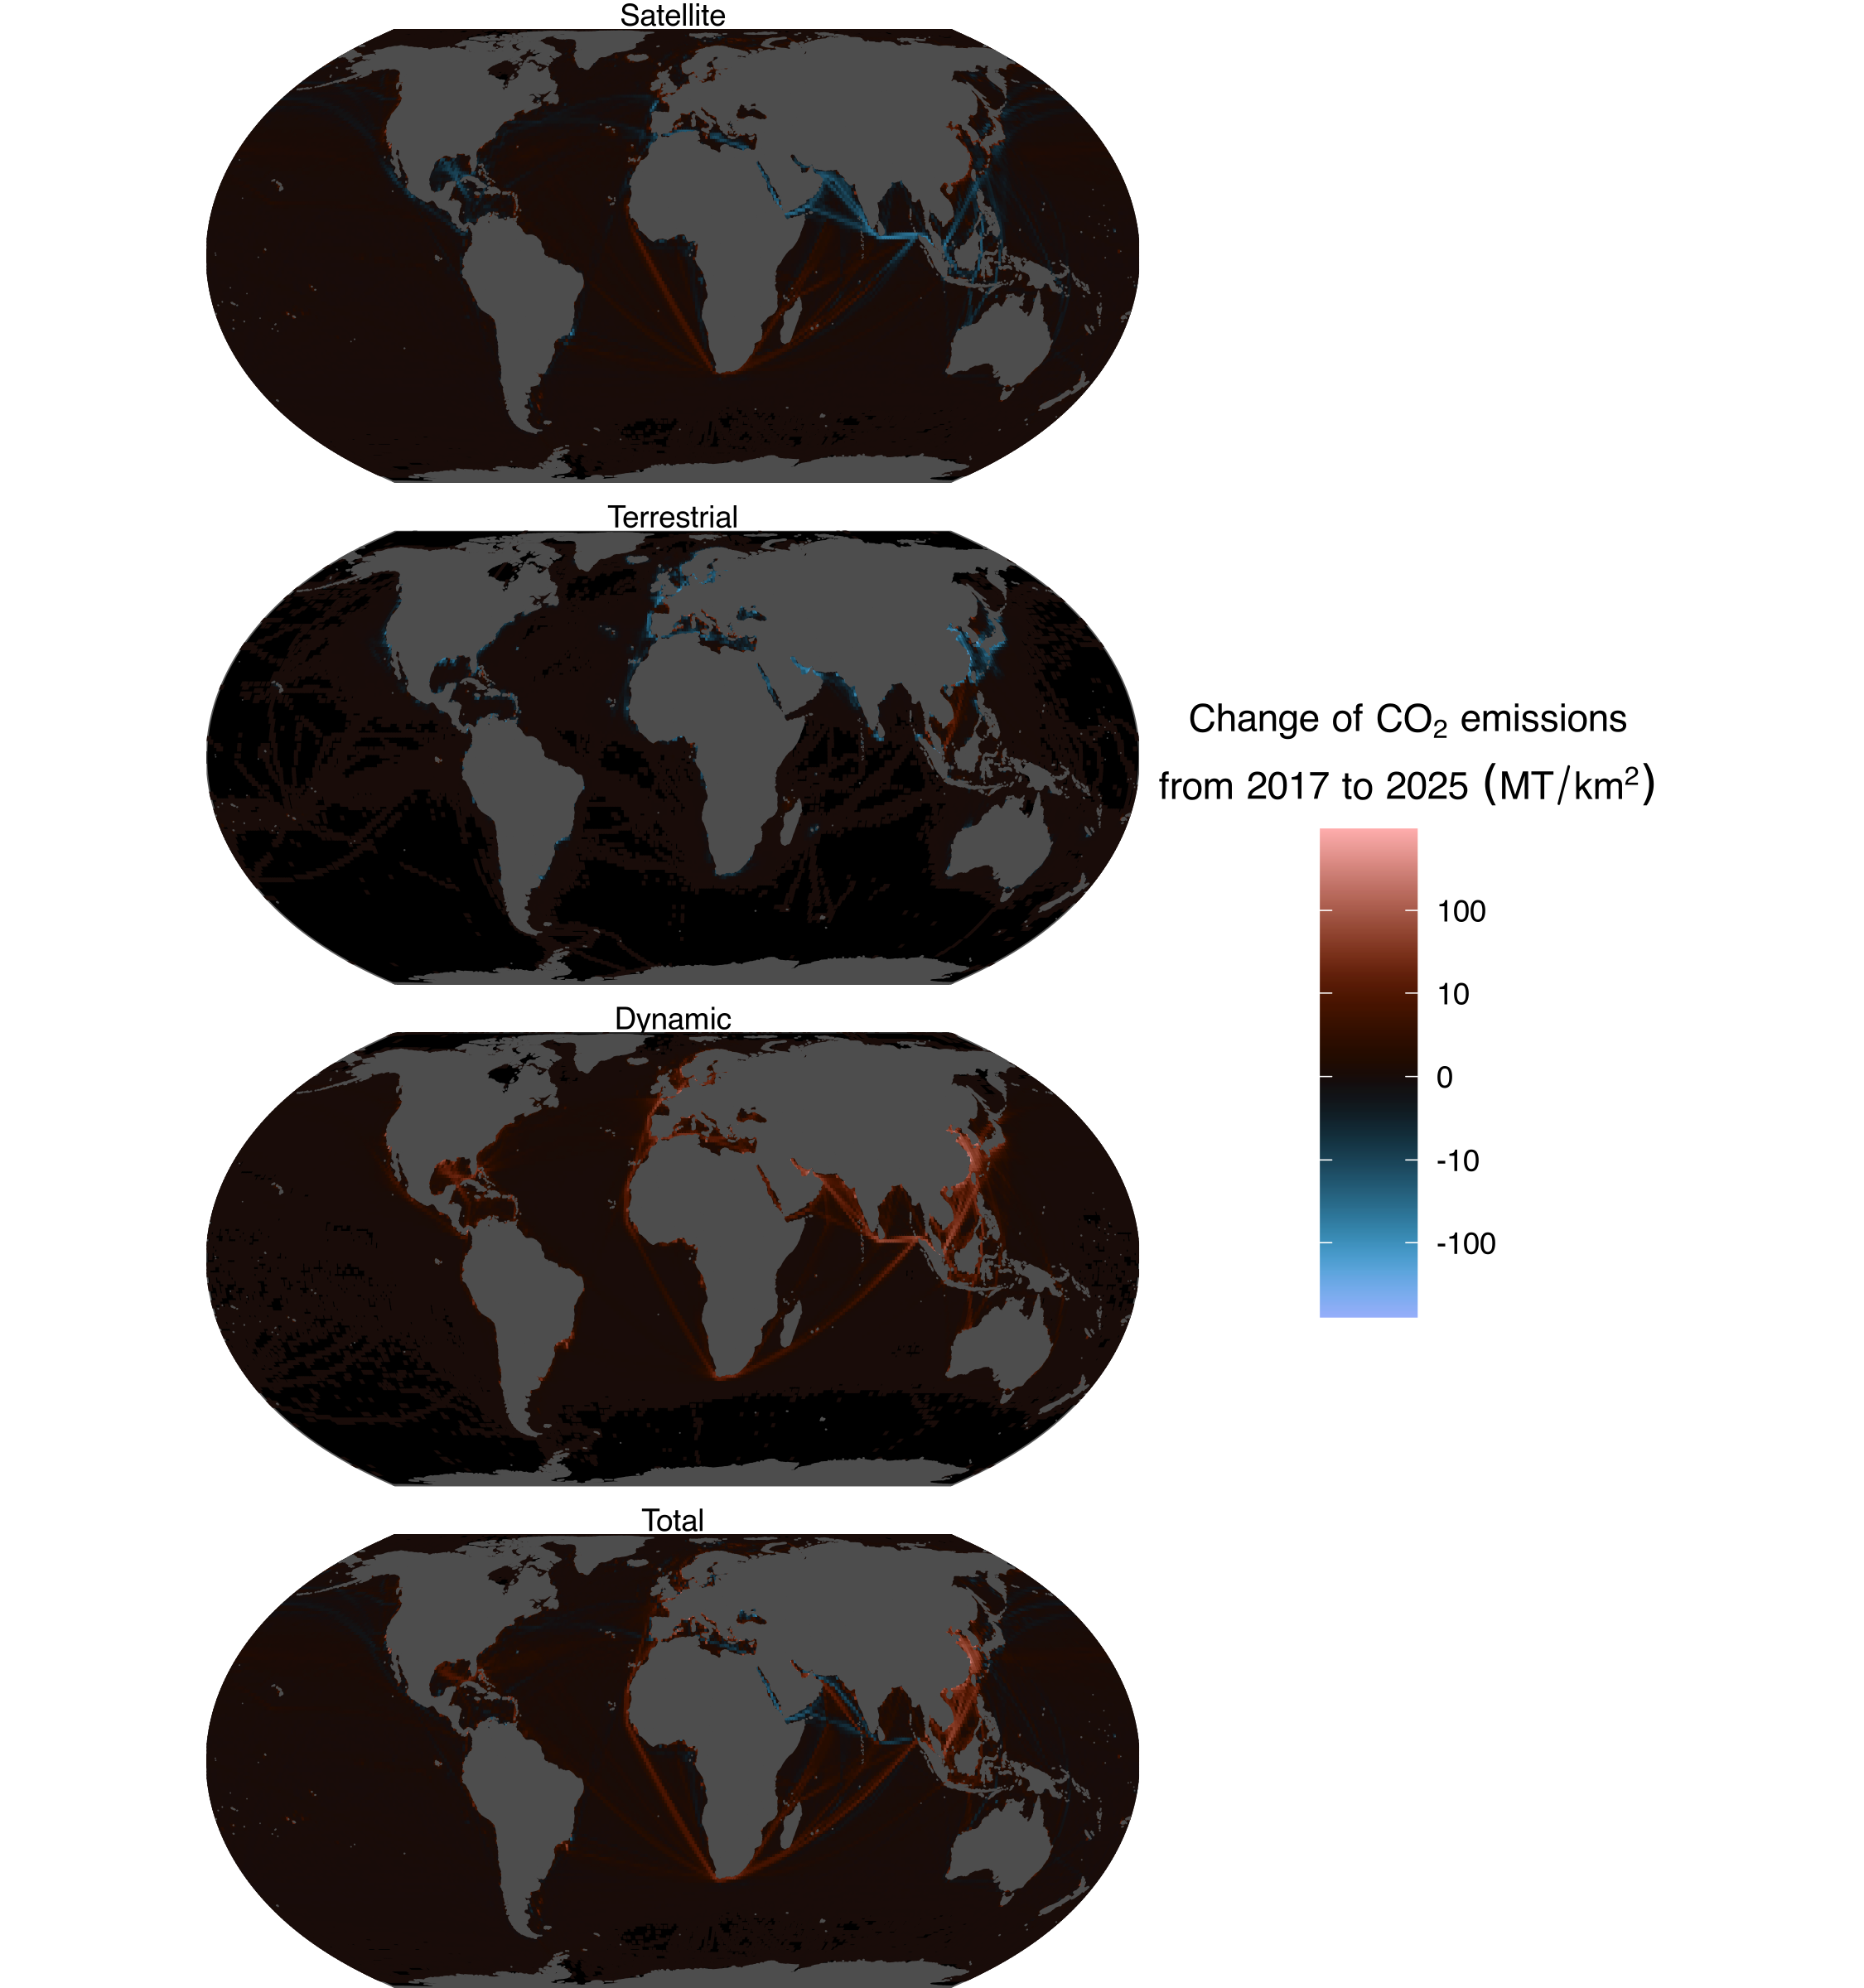
\includegraphics[width=\columnwidth]{figures/fig-co2-emissions-change-map-by-receiver-type-1.png}
    \caption{Spatial change in CO$_{2}$ emissions by AIS-broadcasting vessels between 2017 and 2025 (metric tonnes) by receiver type (satellite, terrestrial, and dynamic) and total across receiver types, at a 1x1 degree spatial resolution; emissions are area-normalized for each pixel (metric tonnes per square kilometer, shown on a pseudolog-10 scale).}
    \label{fig:fig-co2-emissions-change-map-by-receiver-type}
\end{figure}


\supnote{Systematic comparison of our AIS-based emissions modeling methodology to other AIS-based inventories}{sec:methods-comparison}

\subsubsection*{Scope of the comparison and modeling approaches}

Global vessel emission estimates fall into two methodological families, distinguished by whether emissions are derived from aggregate country-level fuel use statistics (i.e., `top-down') or from the observed activity of individual vessels (i.e., `bottom-up'). Top-down, fuel-based inventories combine reported marine fuel sales with fleet-wide emissions factors, without using data on individual vessels. They are unable to estimate vessel-level emissions or assign emissions with high spatiotemporal precision, and are known to underestimate emissions relative to activity-based inventories \cite{miolaEstimatingAirEmissions2011}. Bottom-up, activity-based approaches instead derive emissions mechanistically from the observed movement of individual vessels, calculating the pollutants emitted by each vessel in a specific spatial context and aggregating over time and fleet \cite{nunesActivitybasedMethodologyAssess2017}. 

Since the widespread adoption of AIS, which resolves vessel activity and operational mode at high spatial and temporal resolution, bottom-up AIS-based models have become the reference methodology for global inventories and the approach adopted by the IMO \cite{fourth2020greenhouse}. We therefore build on an extensive body of work and literature that has been developed over the last several decades. The most recent and representative global bottom-up inventories include:

\begin{itemize}
    \item Ship Traffic Emissions Assessment Model (STEAM) \cite{jalkanen2009modelling, jalkanenExtensionAssessmentModel2012, bergShipEmissionsSO22012, johanssonGlobalAssessmentShipping2017, majamaki2025improving}
    \item Shipping Emission Inventory Model (SEIM) \cite{wangShipEmissionsChina2021, yiHighresolutionGlobalShipping2025}
    \item Maritime Transport Environmental Assessment Model (MariTEAM) \cite{kramelGlobalShippingEmissions2021}
    \item the OECD's latest bottom-up model update (hereafter `OECD') \cite{clarke2023co2, oecdMaritimeTransportCO2Methodology2025}
    \item the SAVE model developed by the ICCT (hereafter `SAVE') \cite{olmer2017greenhouse, documentationV2025031Documentation, mao2025greenhouse}, and
    \item the model used for the Fourth IMO GHG Study (`IMO' in figures and tables) \cite{fourth2020greenhouse}.

\end{itemize}

In the following sections, we will compare our AIS-based emissions model to each of these existing inventories. Any AIS-based inventory is assembled from four components, and the differences between these components affect the scope, resolution, and accuracy of each inventory. First, the AIS record itself, which determines which vessels and which movements are observed at all. Second, a vessel-characteristics dataset supplying the parameters the model requires. Third, an engine model converting observed speed into instantaneous main engine load, plus assumptions on auxiliary engine and boiler demand. Fourth, fuel consumption and pollutant specific emission factors, conditioned on engine type, fuel type and the regulation in force at the time and place of the emission. Supplementary Data 1, 2 and 3 compare our methods, input data, and outputs, respectively, against each of the inventories listed above. We end with a comparison of how each inventory is validated against external data sources, and what this tells us about the accuracy of each inventory.

\subsubsection*{Activity and vessel-characteristics data}

All seven inventories are global in spatial extent, so the differences lie in AIS coverage, fleet size, and temporal coverage rather than in geographic scope (Supplementary Data 2). The inventories diverge substantially in the number of vessels represented. Restricting the comparison to vessels explicitly modeled from observed AIS activity, we model 864,738 unique vessels, an average of 396,221 vessels per year rising from 249,732 in 2015 to 529,848 in 2025. This exceeds the AIS-modeled fleet of the Fourth IMO GHG Study, OECD, SAVE, MariTEAM and SEIM. Our fleet size is only comparable to the STEAM inventory, which reported 376,219 vessels in 2015, exceeding our fleet size for the same year. However, STEAM does not report fleet sizes in subsequent updates, preventing a direct comparison for the later years in which our fleet is larger.

The difference with STEAM is also reflected in the underlying AIS data, which used approximately 7.8 billion AIS positions in 2015, compared with approximately 2.3 billion in our 2015 dataset after data cleaning. Our own message volume increases to approximately 26.5 billion positions by 2025, totaling approximately 125 billion positions over the study period (an average of 11.4 billion per year), reflecting the expansion of terrestrial and satellite AIS. Among the remaining inventories, SEIM and MariTEAM report lower AIS message volumes, and the others do not indicate message counts. The increase in AIS messages also reflects the differences in the AIS data types available to us. Terrestrial and satellite AIS constitute the core AIS data types. In addition, GFW obtains a data add-on for both class A and class B D-AIS (also marketed as shipborne AIS), released by the data provider Spire since 2022, which further increases the density and coverage of our AIS record. To our knowledge, D-AIS is generally not included in base AIS data products from most providers, and the inventories covering 2022 onward report conventional AIS data types without indicating whether D-AIS is included, so we cannot determine whether the differences arise from the input data or from a lack of reporting. Of the inventories compared, only OECD (2019 onward) and SAVE (2016-2023) extend into the D-AIS era at all; STEAM's update ends in 2021, SEIM in 2021, the Fourth IMO GHG Study in 2018, and MariTEAM is a single-year 2017 inventory. The question of whether D-AIS inflates our recent trend relative to the others therefore applies to two of the six comparisons. 

Temporal coverage differs in extent. STEAM and MariTEAM are single-year inventories (2015 and 2017 respectively), with STEAM subsequently updated through 2021 to account for ambient conditions \cite{majamaki2025improving}. SEIM covers 2013 and 2016--2021, the Fourth IMO GHG Study 2012--2018, SAVE 2016--2023, and OECD from 2019 onward. Our use of consistent GFW AIS products, though input density evolves, enables a continuous AIS-based inventory from 2015, and an AIS-based plus S1-unmatched inventory from 2017, to the present without methodological discontinuities.

Every inventory uses official registries as the primary source of vessel characteristics and applies gap-filling where information is unavailable. The differences are in how far the registry is extended and how the remainder is inferred. The simplest filling approaches substitute central tendencies. The OECD restricts to vessels matching between commercial and public registries and imputes from vessel class and size group means \cite{oecdMaritimeTransportCO2Methodology2025}, while SAVE fills missing characteristics from average values \cite{documentationV2025031Documentation}. STEAM retains some of the within-class variation by replicating the characteristics of a similar vessel already listed in its database \cite{johanssonGlobalAssessmentShipping2017}. MariTEAM fills gaps with regression models, though its modeled fleet is restricted to the registered fleet \cite{kramelGlobalShippingEmissions2021}, while the Fourth IMO GHG Study applies similar regressions as its primary method and falls back to class and size medians, on a dataset expanded with registered and public datasets \cite{fourth2020greenhouse}. Of the published inventories, SEIM is the only one besides ours to describe a more involved machine-learning approach to infer missing vessel characteristics, applied after extending commercial registries with open data \cite{yiHighresolutionGlobalShipping2025}. In our vessel information dataset, characteristics are taken from data purchased from S\&P Global, from publicly available official registries consolidated through extensive prior scraping work \cite{park2023tracking}, and where neither is available, from inferred characteristics. Building on \cite{kroodsma2018tracking}, these are inferred with new random-forest models trained on commercial registry data (Section \ref{sec:vessel-characteristics-models}). This enables the inclusion of a substantially larger number of vessels than most previous studies, reaching a fleet dominated by small domestic and fishing vessels that the more registry-anchored inventories cannot represent.

Finally, the inventories differ in how they treat vessels absent from the AIS feed. STEAM, SEIM and MariTEAM rely exclusively on AIS or port-call data and make no allowance for unobserved activity. OECD, SAVE and the Fourth IMO GHG Study impute activity and emissions for small registered vessels missing from AIS, scaling from explicitly modeled vessels of the same type and size. Both approaches are bounded by the registry, where imputation can only recover a vessel that some registry lists. We instead estimate S1-unmatched emissions, from vessels detected in S1 SAR imagery that cannot be matched to an AIS broadcast, using machine learning and data fusion (Section \ref{sec:non-broadcasting-vessels}), which recovers vessel activity that does not appear in AIS, both for vessels that simply do not carry AIS transponders at all, and also for vessels that carry AIS transponders but whose signal is not received. To our knowledge this is the first global shipping inventory to do so.

\subsubsection*{Engine and emissions model}

Every AIS-based inventory estimates the propulsion energy required by the main engine to overcome hull resistance at the observed vessel speed, and the models differ in the resolution at which the components of that resistance are resolved. The literature defines two main modeling approaches: load-based (i.e., SEIM, SAVE, OECD, the Fourth IMO GHG Study, and our study) and resistance-based (i.e., STEAM and MariTEAM). While load-based models are regarded as adequate approximations of more complex methods, resistance-based models are often avoided because of the number of inputs needed. Resistance models require hull parameters, which restricts their applicability to vessels with such documented information in the registries. Imputing class-average hull parameters may be acceptable for fleet-level aggregates and well-defined classes with limited variation in hull design, but performance declines for underrepresented and heterogeneous classes and can substantially alter single-vessel estimates \cite{brownPowerModelsAverage2019}. This limitation is particularly relevant because we model a broader fleet dominated by small domestic and fishing vessels, for which hull geometry is often absent or incomplete, and report emissions at a finer resolution, by trip and by vessel. The resistance model's advantage in physical realism would therefore be offset by uncertainty in its inputs. The load-based formulation, by contrast, requires only installed main engine power, design speed, observed speed and a small number of further characteristics that are readily available in registries and can be modeled with confidence where they are not. As in the other load-based models, correction factors are then applied to main engine load. Draft corrections are applied at a lower resolution than in \cite{fourth2020greenhouse}, \cite{documentationV2025031Documentation} and \cite{oecdMaritimeTransportCO2Methodology2025}, as draft is not reliably reported in our AIS records; weather and fouling corrections follow comparable approaches to the other load-based models; and a new correction is introduced to account for fishing activity.

For engine and fuel parameterization, we adapted the methods of the Fourth IMO GHG Study \cite{fourth2020greenhouse}, which established the standard assumptions now adopted by most shipping emissions models. Building an expanded activity dataset around a community reference also allows us to attribute differences from existing inventories to fleet coverage and activity representation, the claim this paper makes. Deviations from those methods depended on data availability or the quality of inferred values, but remain in line with other load-based models \cite{yiHighresolutionGlobalShipping2025, oecdMaritimeTransportCO2Methodology2025, documentationV2025031Documentation}. Specific fuel oil consumption (SFOC) and the decomposition of emissions into main engine, auxiliary engine and boiler components follow the general consensus across models \cite{fourth2020greenhouse, yiHighresolutionGlobalShipping2025, oecdMaritimeTransportCO2Methodology2025, documentationV2025031Documentation}, including the resistance-based ones \cite{johanssonGlobalAssessmentShipping2017, kramelGlobalShippingEmissions2021} (Supplementary Data 1). Our approach is more limited in its treatment of fuel types, which are not explicitly modeled because vessel-level fuel type data are unavailable. For a given engine type, SFOC values and emission factors are therefore calculated as the average across the fuel types associated with that engine type. LNG was not included as a fuel type, given the very limited number of vessels that currently use it and the vastly different emission factors it produces. Our treatment of policy instruments is also narrower than that of comparable models, which apply fuel-sulfur and NOx limits geographically within Emission Control Areas (ECAs) \cite{johanssonGlobalAssessmentShipping2017, yiHighresolutionGlobalShipping2025, fourth2020greenhouse, documentationV2025031Documentation}; STEAM and SAVE additionally account for technologies such as scrubbers and dual-fuel operation. Our NOx limits are assigned by engine Tier from build year and engine speed but are not resolved spatially by NOx ECA boundaries, and SOx and PM estimates are expected to be biased upward within ECAs, an effect concentrated before 2020, when the difference between ECA and global sulfur limits was largest.

\subsubsection*{Differences in validation}

Validation of existing inventories has rested largely on aggregate benchmarking against independent statistics, top-down approaches and against other bottom-up inventories. Our global totals were cross-compared against all six inventories discussed here, and against the multisector EDGAR and CEDS inventories \cite{guizzardiGlobalUptoDate2025, hoeslyHistorical17502014Anthropogenic2018}. As for the other models, STEAM benchmarked global fuel use against IEA statistics and the Third IMO GHG Study, modeled maritime transport work against UNCTAD seaborne-trade statistics and regional results against the EMEP inventory. SEIM, which rests entirely on this class of evidence, compares global totals and trends against EDGAR, CEDS and the Fourth IMO GHG Study, with an activity and fleet benchmark against UNCTAD. MariTEAM cross-compares against the Fourth IMO GHG Study for the same year and STEAM3 for a different year. OECD is the most extensive in this respect, benchmarking global totals against IEA and the Fourth IMO GHG Study, fleet activity against UNCTAD, average efficiencies by class and size against IMO for 2018, and country-level results against national Air Emission Accounts for more than 35 countries. SAVE benchmarks aggregated fuel consumption against IMO DCS for vessels of 5,000 GT and above, and the Fourth IMO GHG Study against the Third IMO GHG Study, their own top-down estimates, the ICCT inventory, and global fuel sales reported by the IEA and UNSD.

Although comparing aggregate emissions totals against other inventories can be illustrative, it does not provide information on how well a model can estimate emissions for a particular vessel; this requires comparison against independent \textit{vessel-level} emissions or fuel use data. We validate against two such datasets: vessel-specific measured fuel consumption for 15,679 unique vessels from a proprietary vessel registry dataset, and EU MRV records covering 20,432 vessel-years. To our knowledge, this is the largest vessel-level validation of a global bottom-up shipping inventory. Other validations using in situ measurements include that of the Fourth IMO GHG Study, which compares yearly estimates against 9,739 vessel records in the 2018 EU MRV dataset and additionally draws on engine power and fuel consumption measurements from 94 vessels' Continuous Monitoring Dataset \cite{fourth2020greenhouse}. SAVE also validates per-vessel-year carbon intensity against EU MRV \cite{documentationV2025031Documentation}. OECD likewise draws on EU MRV, but compares totals aggregated by vessel class rather than by individual vessel \cite{oecdMaritimeTransportCO2Methodology2025}. MariTEAM validates modeled engine power against in situ measurements for a single vessel \cite{kramelGlobalShippingEmissions2021}. STEAM was validated in earlier versions against a limited sample of in situ measurements \cite{bergShipEmissionsSO22012}, and its recent ambient-conditions update validates modeled fuel consumption against 6,445 vessel-year records in the EU MRV data \cite{majamaki2025improving}. This last comparison bears directly on the choice of propulsion formulation (i.e., load-based and resistance-based). Applied to an identical fleet and AIS record, resistance-based methods have been reported to yield lower fleet-level CO$_{2}$ than their load-based equivalents \cite{brownPowerModelsAverage2019}, but that offset has so far been established only between models, or against limited samples of in situ measurements \cite{bergShipEmissionsSO22012, kramelGlobalShippingEmissions2021}. Here the two families, represented by STEAM and our model, are each tested against the same independent benchmark dataset (i.e., EU MRV) and perform comparably, both achieving an R$^{2}$ of approximately 0.8 \cite{majamaki2025improving}, supporting our methodological choices and indicating that the load-based formulation as implemented here does not exhibit the systematic upward bias reported by \cite{brownPowerModelsAverage2019}.


\supnote{Systematic comparison of our emissions magnitude and trend estimates to other inventories}{sec:inventory-comparison}

Validation against the registered and EU MRV datasets tests the emissions model vessel by vessel, but says nothing about whether the modeled fleet is complete. Benchmarking against independent inventories tests that. Below we compare the magnitude and the trend of our estimates against the activity-based inventories introduced in Section \ref{sec:methods-comparison}, and then against the fuel-statistics-derived inventories EDGAR and CEDS. Each comparison is limited to what each inventory reports publicly.

\subsubsection*{Comparing our estimates with other bottom-up inventories}

Our AIS-based estimates agree closely with the other activity-based inventories (STEAM, SEIM, MariTEAM, OECD, SAVE, and the Fourth IMO GHG Study) over the first years of the study period (Fig. \ref{fig:fig-emissions-inventory-comparison}, panel a, tabulated in Supplementary Table \ref{tab:inventory_comparison_all_sources}). This closeness in total emissions coexists with substantial disagreement in fleet scope and AIS coverage, among the other inventories as much as between them and ours, so it does not reflect agreement on fleet extent. Rather, all of these inventories rest on a registry-matched core of roughly 45,000-90,000 large vessels that accounts for most emissions \cite{fourth2020greenhouse, yiHighresolutionGlobalShipping2025, oecdMaritimeTransportCO2Methodology2025, documentationV2025031Documentation, johanssonGlobalAssessmentShipping2017, kramelGlobalShippingEmissions2021}. In our inventory, registry-matched vessels likewise produced 78\% of AIS-based CO$_{2}$ in 2017 while making up 30\% of broadcasting vessels. Differences in totals therefore reflect how much of the low-information tail of smaller and unregistered vessels each inventory includes, together with the methodological choices described in Section \ref{sec:methods-comparison}. Our per-vessel emissions fall within the range of the other models, at 2.3 kt CO$_{2}$ per vessel per year across all broadcasting vessels and 6.08 kt across registry-matched vessels alone, against 2.33 to 7.90 kt for the other inventories (MariTEAM aside, at 20.6 kt), so the differences are in fleet scope rather than in emissions per vessel.

\begin{figure}[H]
    \centering
    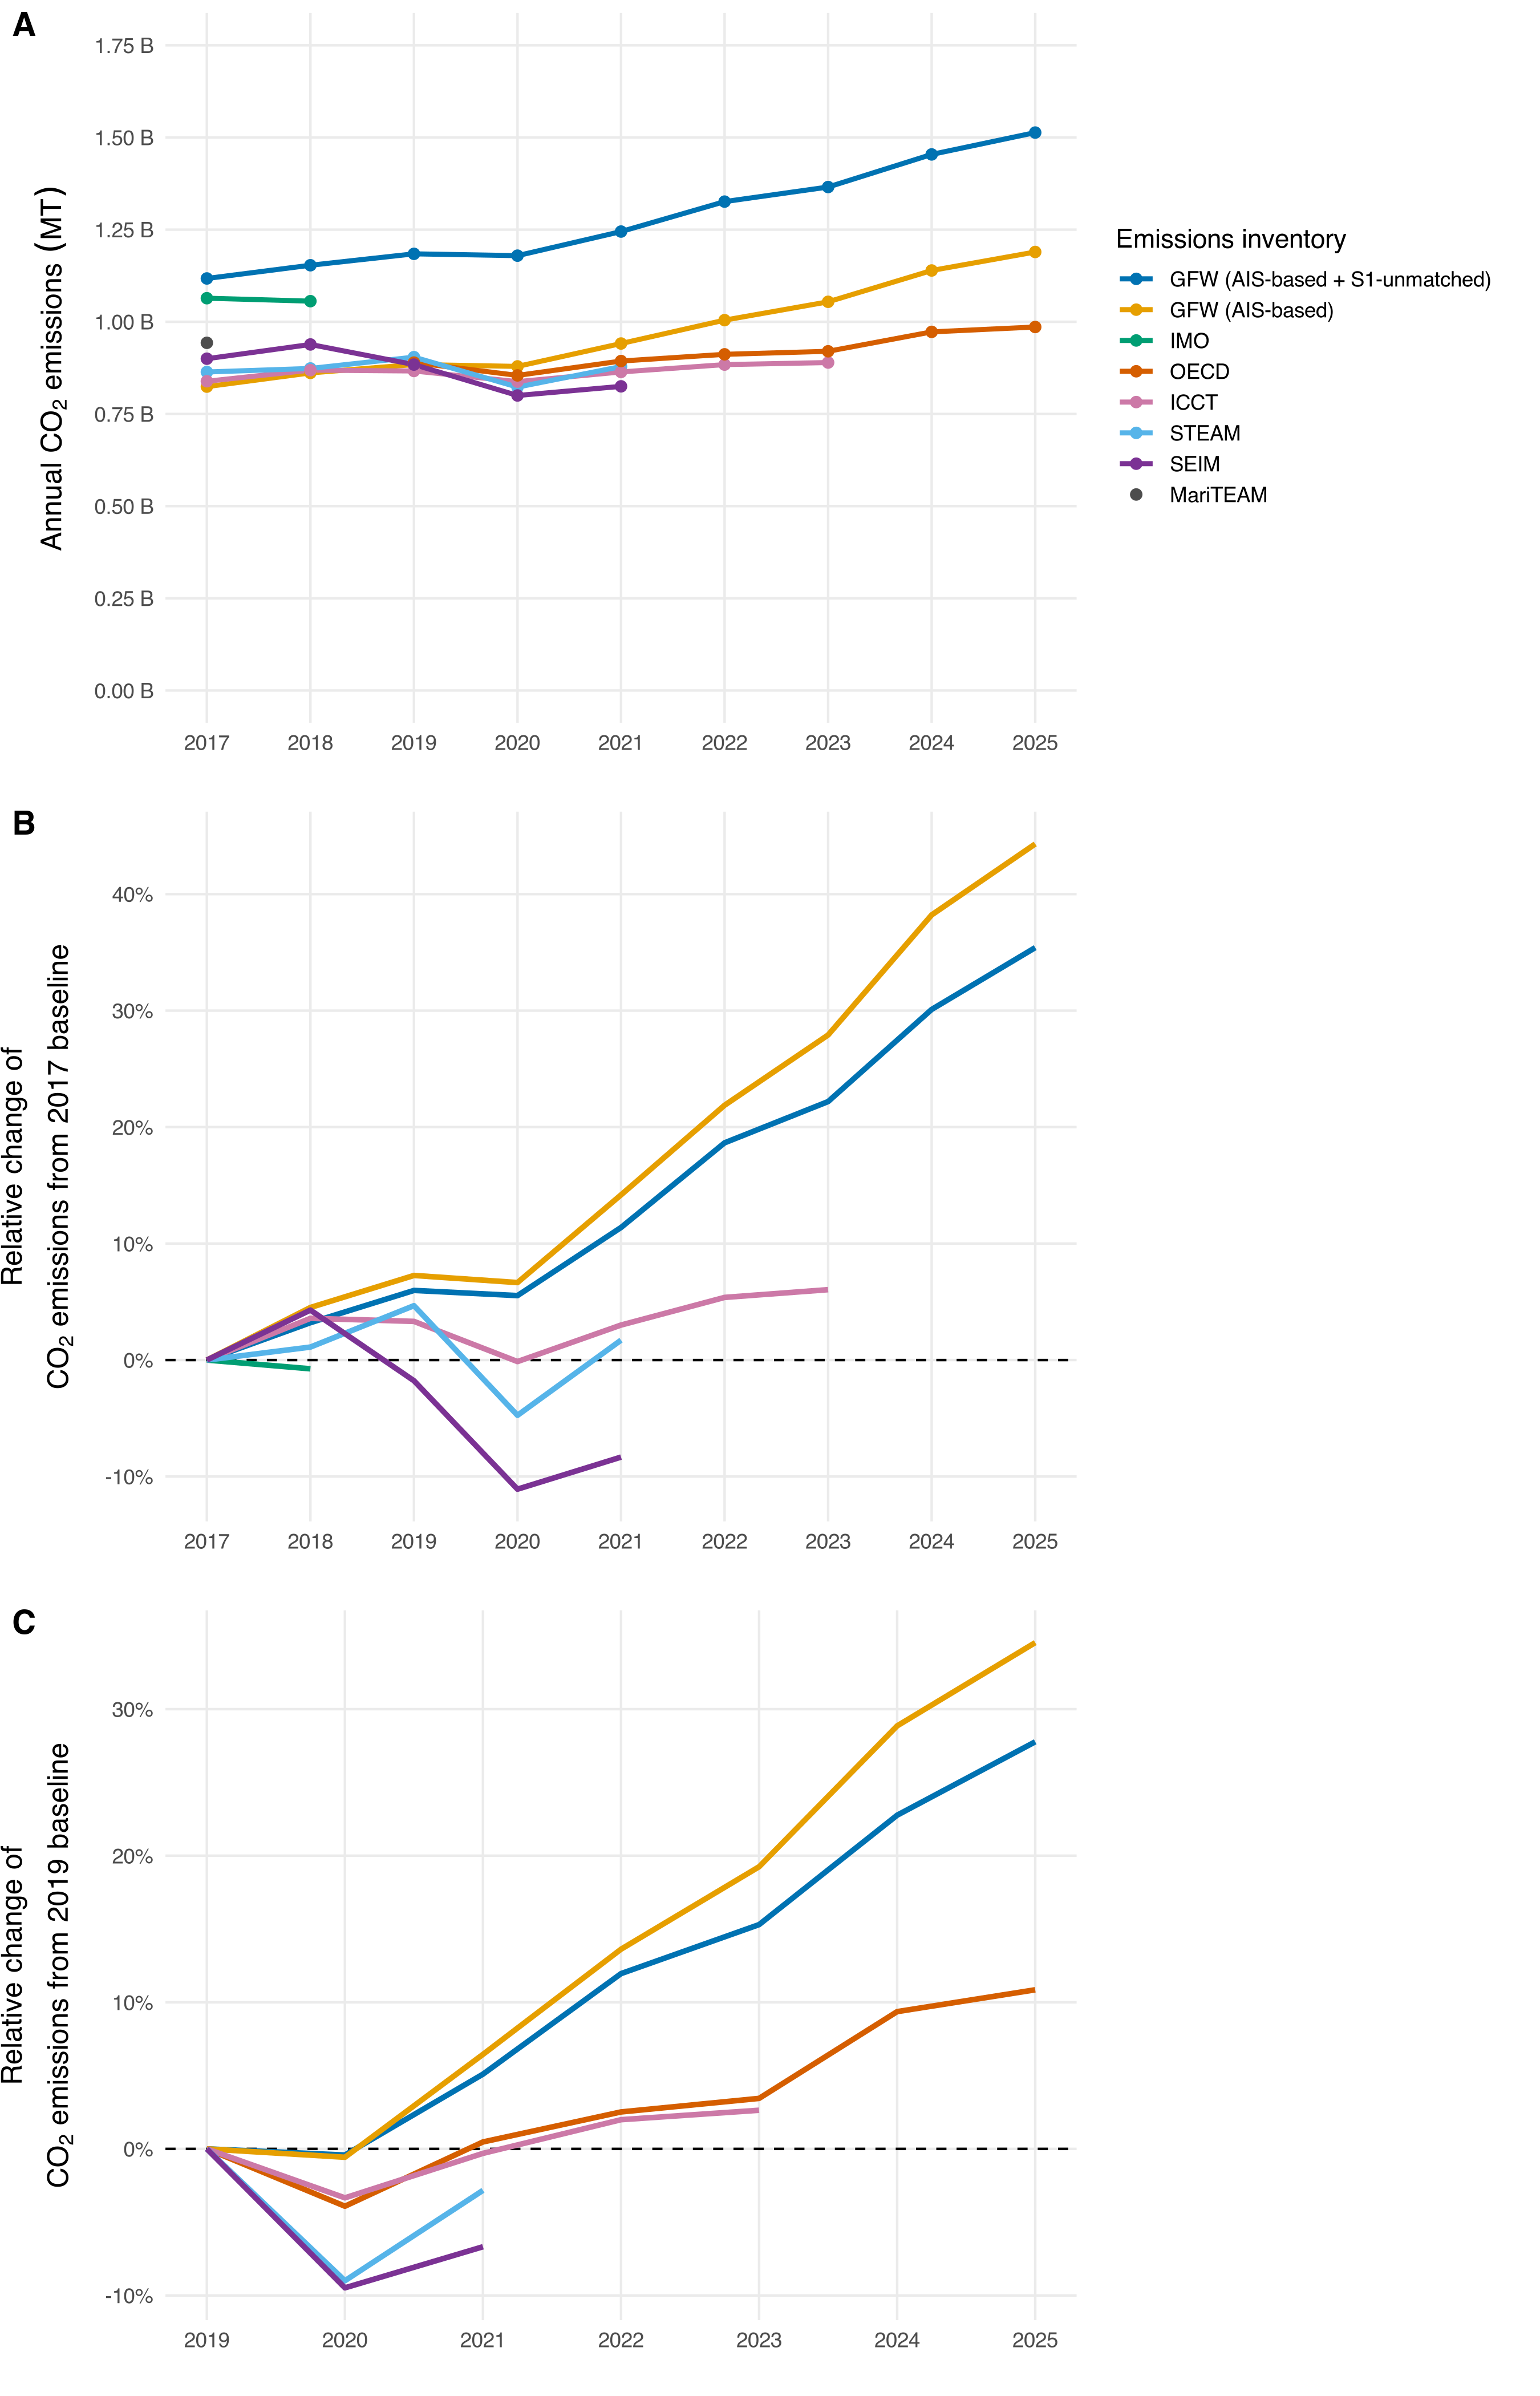
\includegraphics[width=\columnwidth]{figures/figS-inventory-comparison-all-sources-1.png}
    \caption{Trends in our AIS-based and fused estimates against other inventories. (a, b) Change relative to 2017 and to 2019, respectively, against the published bottom-up inventories; the later baseline admits OECD, whose series begins in 2019. (c) Change relative to 2017 against the top-down EDGAR and CEDS inventories, for shipping, all other transportation modes, and all sectors. (d) Our AIS-based series split into registry-matched and unmatched vessels, relative to 2017, with the fragment of vessels 150 m and above for comparison.}
    \label{fig:figS-inventory-comparison-all-sources}
\end{figure}

% Nine columns overflow the text block at the default column padding
\begingroup
\setlength{\tabcolsep}{2.5pt}
\begin{table}[!h]
\centering
\caption{\label{tab:inventory_comparison_all_sources}Annual marine vessel CO$_{2}$ emissions (billions of metric tonnes) for our AIS-based and fused (AIS-based + S1-unmatched) estimates and for the published bottom-up, activity-based inventories. A dash marks a year for which an inventory publishes no estimate.}
\centering
\fontsize{7}{9}\selectfont
\setlength{\tabcolsep}{3pt}
\begin{tabular}[t]{r|l|l|l|l|l|l|l|l}
\hline
Year & \shortstack{GFW\\(AIS-based +\\S1-unmatched)} & \shortstack{GFW\\(AIS-based)} & IMO & OECD & SAVE & STEAM & SEIM & MariTEAM\\
\hline
2017 & 1.065 & 0.824 & 1.064 & - & 0.839 & 0.864 & 0.900 & 0.943\\
\hline
2018 & 1.098 & 0.861 & 1.056 & - & 0.869 & 0.874 & 0.939 & -\\
\hline
2019 & 1.128 & 0.884 & - & 0.889 & 0.867 & 0.904 & 0.884 & -\\
\hline
2020 & 1.122 & 0.879 & - & 0.855 & 0.838 & 0.823 & 0.800 & -\\
\hline
2021 & 1.187 & 0.941 & - & 0.894 & 0.864 & 0.879 & 0.825 & -\\
\hline
2022 & 1.259 & 1.005 & - & 0.912 & 0.884 & - & - & -\\
\hline
2023 & 1.299 & 1.054 & - & 0.920 & 0.890 & - & - & -\\
\hline
2024 & 1.384 & 1.139 & - & 0.973 & - & - & - & -\\
\hline
2025 & 1.443 & 1.189 & - & 0.986 & - & - & - & -\\
\hline
\end{tabular}
\end{table}

\endgroup
\FloatBarrier

In the most recent years our AIS-based series grows faster than every other inventory (Supplementary Fig. \ref{fig:figS-inventory-comparison-all-sources}, panels a and b). The difference lies in how the fleets are defined. Inventories constrained by commercial registries change primarily at the pace of registry updates and activity of vessels within the registry, whereas our fleet is defined by AIS observation and grows with AIS carriage. Our broadcasting fleet accordingly grows faster than the OECD and SAVE fleets, the only inventories publishing vessel counts over the recent period, and the growth is carried entirely by vessels that cannot be matched to a registry: their AIS-based emissions nearly quadrupled between 2017 and 2025 while emissions from registry-matched vessels fell by 27\% (Supplementary Fig. \ref{fig:figS-inventory-comparison-all-sources}, panel d), so that unmatched vessels went from 22\% to 60\% of our AIS-based CO$_{2}$. S1 detections show the mechanism directly. Among detected large non-fishing vessels, the segment where AIS carriage is mandated and registry coverage is strongest, the share with no matching AIS broadcast is essentially unchanged since 2017, whereas it falls steeply among small non-fishing and fishing vessels as AIS carriage and reception expand (Supplementary Fig. \ref{fig:figS-ais-carriage-saturation-by-size}). Consistently, the largest emissions growth in our AIS-based series comes from small passenger vessels and from fishing vessels (Supplementary Fig. \ref{fig:figS-passenger-size-panels} and Supplementary Fig. \ref{fig:figS-fleet-sankey-with-series-2025}), fleets of numerous small, largely coastal vessels that registries cover poorly and that enter the model only as they begin to broadcast. The phase-in of D-AIS (Section \ref{sec:ais-receiver-types}) adds a second, smaller effect: AIS positions received more than doubled between 2021 and 2025 while observed distance traveled and AIS-based emissions rose together by only $\sim$27\%, so D-AIS mostly densified trajectories that were already observed rather than adding new activity. The divergence from the other inventories therefore does not indicate that our totals are inflated. It indicates that the other inventories, and our own early years, miss part of the fleet, and that any AIS-based trend partly measures the expansion of AIS carriage rather than of activity at sea. We return to this second point below.

\begin{figure}[H]
    \centering
    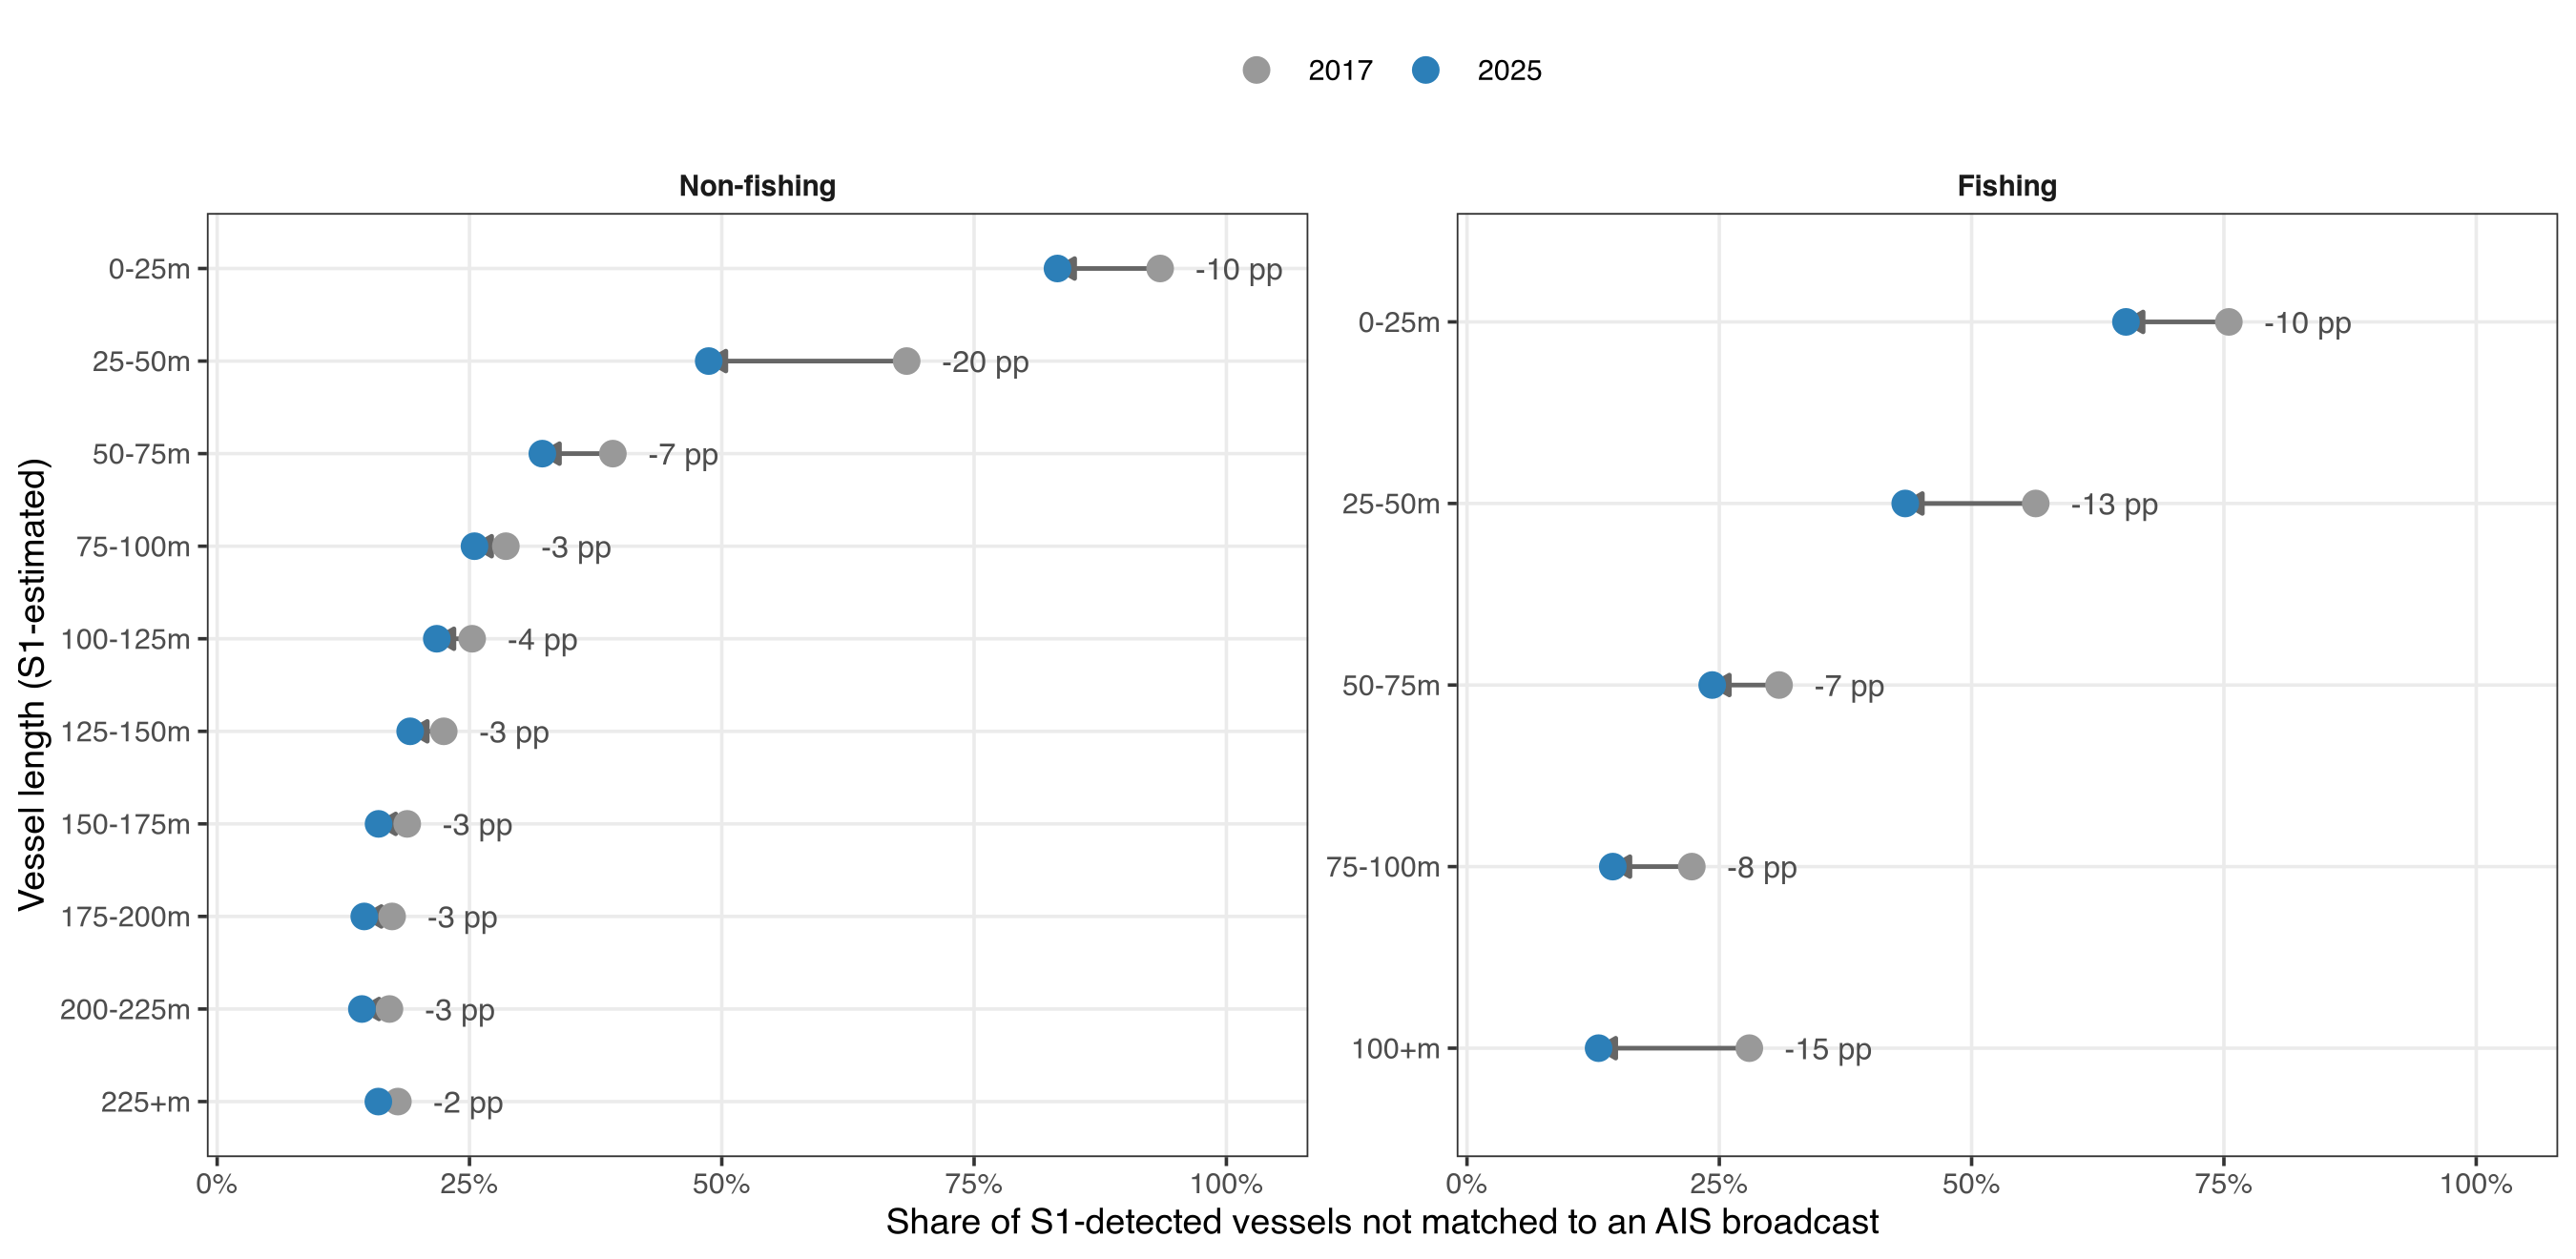
\includegraphics[width=\columnwidth]{figures/figS-ais-carriage-saturation-by-size-1.png}
    \caption{AIS carriage saturation by vessel size: share of S1 detections with no matching AIS broadcast, by length bin, 2017 against 2025. The unmatched share is flat for the largest vessels and falls steeply for the smallest.}
    \label{fig:figS-ais-carriage-saturation-by-size}
\end{figure}

Our fused total (AIS-based plus S1-unmatched) sits above every other inventory across the whole period (Fig. \ref{fig:fig-emissions-inventory-comparison}, panel a) because it extends the fleet through satellite imagery-based detections to vessels that appear in neither registries nor AIS. The Fourth IMO GHG Study, OECD, and SAVE also attempt to account for non-broadcasting vessels by assigning small registered vessels without AIS signals the activity profiles of explicitly modeled vessels, yet only the IMO study approaches our total: an inventory anchored to a registry can reach no further than the registry itself.

\subsubsection*{Comparing our estimates with top-down inventories}

We also compared our fused estimates against two inventories derived from fuel statistics, the Emissions Database for Global Atmospheric Research (EDGAR) and the Community Emissions Data System (CEDS). EDGAR builds its shipping estimate from reported fuel sales, representing international shipping from international marine bunkers and domestic activity from domestic navigation fuel statistics, with recent years extrapolated from Energy Institute fuel oil trends \cite{guizzardiGlobalUptoDate2025}; it can therefore only count fuel that was sold and reported. CEDS starts from the same fuel statistics but treats them as systematically under-reported and scales its global shipping total to bottom-up estimates, mainly the IMO GHG Studies \cite{hoeslyHistorical17502014Anthropogenic2018, ceds_data_and_assumptions}, so it also inherits the fleet-scope limits described above. Our fused total exceeds both (Fig. \ref{fig:fig-emissions-inventory-comparison}, panel b, tabulated in Supplementary Table \ref{tab:multisector_shipping_comparison}). The gap in magnitude and the gap in trend have different causes.

\begin{table}[!h]
\centering
\caption{\label{tab:multisector_shipping_comparison}Annual marine vessel CO$_{2}$ emissions (billions of metric tonnes) for our AIS-based and fused (AIS + S1) estimates against the shipping sector of the top-down EDGAR and CEDS inventories, whose shipping scope combines international and domestic navigation. A dash marks a year for which an inventory publishes no estimate.}
\centering
\fontsize{8}{10}\selectfont
\begin{tabular}[t]{r|l|l|l|l}
\hline
Year & GFW (AIS + S1) & GFW (AIS) & EDGAR - Shipping & CEDS - Shipping\\
\hline
2017 & 1.107 & 0.824 & 0.881 & 1.040\\
\hline
2018 & 1.143 & 0.861 & 0.887 & 1.031\\
\hline
2019 & 1.174 & 0.884 & 0.875 & 1.030\\
\hline
2020 & 1.198 & 0.879 & 0.798 & 0.937\\
\hline
2021 & 1.270 & 0.941 & 0.833 & 0.979\\
\hline
2022 & 1.341 & 1.005 & 0.837 & 0.975\\
\hline
2023 & 1.377 & 1.054 & 0.890 & 1.014\\
\hline
2024 & 1.467 & 1.139 & 0.860 & -\\
\hline
2025 & 1.533 & 1.189 & - & -\\
\hline
\end{tabular}
\end{table}

\FloatBarrier

\begin{table}[!h]
\centering
\caption{\label{tab:inventory_growth_comparison}Growth in CO$_2$ emissions for our estimates and for every inventory compared in Supplementary Note \ref{sec:inventory-comparison}. All series are anchored at 2017 where they extend that far back, and because the inventories end in different years each is summarized to its own end year. Growth is reported two ways: the total percent change between the first and last year, and the compound annual growth rate (CAGR). The Fourth IMO GHG Study ends in 2018 and is therefore reported over its native 2015-2018 window, since anchoring it at 2017 would leave a single year-on-year change. MariTEAM is a single-year inventory and admits no growth rate. EDGAR and CEDS changes are shown for All sectors, Other transportation and Shipping scopes.}
\centering
\fontsize{8}{10}\selectfont
\begin{tabular}[t]{l|c|r|r}
\hline
Series & Time window & Total \% change & CAGR (\%/yr)\\
\hline
\multicolumn{4}{l}{\textbf{Ours}}\\
\hline
\hspace{1em}GFW (AIS-based + S1-unmatched) & 2017--2025 & +35.52 & +3.87\\
\hline
\hspace{1em}GFW (AIS-based) & 2017--2025 & +44.31 & +4.69\\
\hline
\hspace{1em}GFW (AIS-based, $\geq$150 m) & 2017--2025 & +28.62 & +3.20\\
\hline
\multicolumn{4}{l}{\textbf{Bottom-up}}\\
\hline
\hspace{1em}IMO & 2015--2018 & +6.56 & +2.14\\
\hline
\hspace{1em}OECD & 2019--2025 & +10.85 & +1.73\\
\hline
\hspace{1em}SAVE & 2017--2023 & +6.04 & +0.98\\
\hline
\hspace{1em}STEAM & 2017--2021 & +1.71 & +0.42\\
\hline
\hspace{1em}SEIM & 2017--2021 & -8.33 & -2.15\\
\hline
\hspace{1em}MariTEAM & 2017 & --- & ---\\
\hline
\multicolumn{4}{l}{\textbf{EDGAR}}\\
\hline
\hspace{1em}All sectors & 2017--2024 & +7.06 & +0.98\\
\hline
\hspace{1em}Other transportation & 2017--2024 & +3.35 & +0.47\\
\hline
\hspace{1em}Shipping & 2017--2024 & -2.38 & -0.34\\
\hline
\multicolumn{4}{l}{\textbf{CEDS}}\\
\hline
\hspace{1em}All sectors & 2017--2023 & +5.60 & +0.91\\
\hline
\hspace{1em}Other transportation & 2017--2023 & +3.27 & +0.54\\
\hline
\hspace{1em}Shipping & 2017--2023 & -2.46 & -0.41\\
\hline
\end{tabular}
\end{table}

\FloatBarrier

The magnitude gap arises from three differences in the fleets these inventories can account for. First, fishing largely falls outside the shipping sector in both. They report fishing fuel combined with agriculture and forestry, so EDGAR's shipping estimate contains no fishing vessels at all, while in CEDS only some unreported fishing fuel is absorbed into global shipping through the bottom-up anchor. Second, small coastal and inland vessels are only partly covered: domestic navigation fuel is intended to capture this traffic, but the sector is inconsistently defined across reporting countries \cite{kuenen2014tno}. Third, neither inventory can capture fuel that never passes through reported channels, affecting vessels supplied informally or illegally. Each of these mechanisms adds emissions the top-down inventories cannot see, and our own detection limits can only mean we understate the total further, so the magnitude gap rests on firm ground.

The trend gap is different in kind. Growth in our AIS-based series partly reflects expanding AIS carriage and coverage, as shown above. The fused total should be less sensitive to that: a vessel that adopts AIS and begins to broadcast moves from the S1-unmatched component to the AIS-based one, reallocating emissions between them rather than adding to the sum. S1 detections, which depend on neither AIS broadcasting nor registration, offer a partial independent check. Detected activity per unit of observing effort stayed roughly flat overall, but its composition shifted, growing among small non-fishing vessels and, most strongly, among the largest, while mid-size classes were flat and fishing declined (Supplementary Fig. \ref{fig:figS-density-by-match-status}, panel a). For the largest vessels, AIS carriage is already near-universal and the unmatched share has barely changed since 2017 (Supplementary Fig. \ref{fig:figS-ais-carriage-saturation-by-size}), so their growth must largely reflect new activity; because a large ship emits on the order of a hundred times what a small one does, that compositional shift matters for emissions even if the total number of vessels did not change.

\begin{figure}[H]
    \centering
    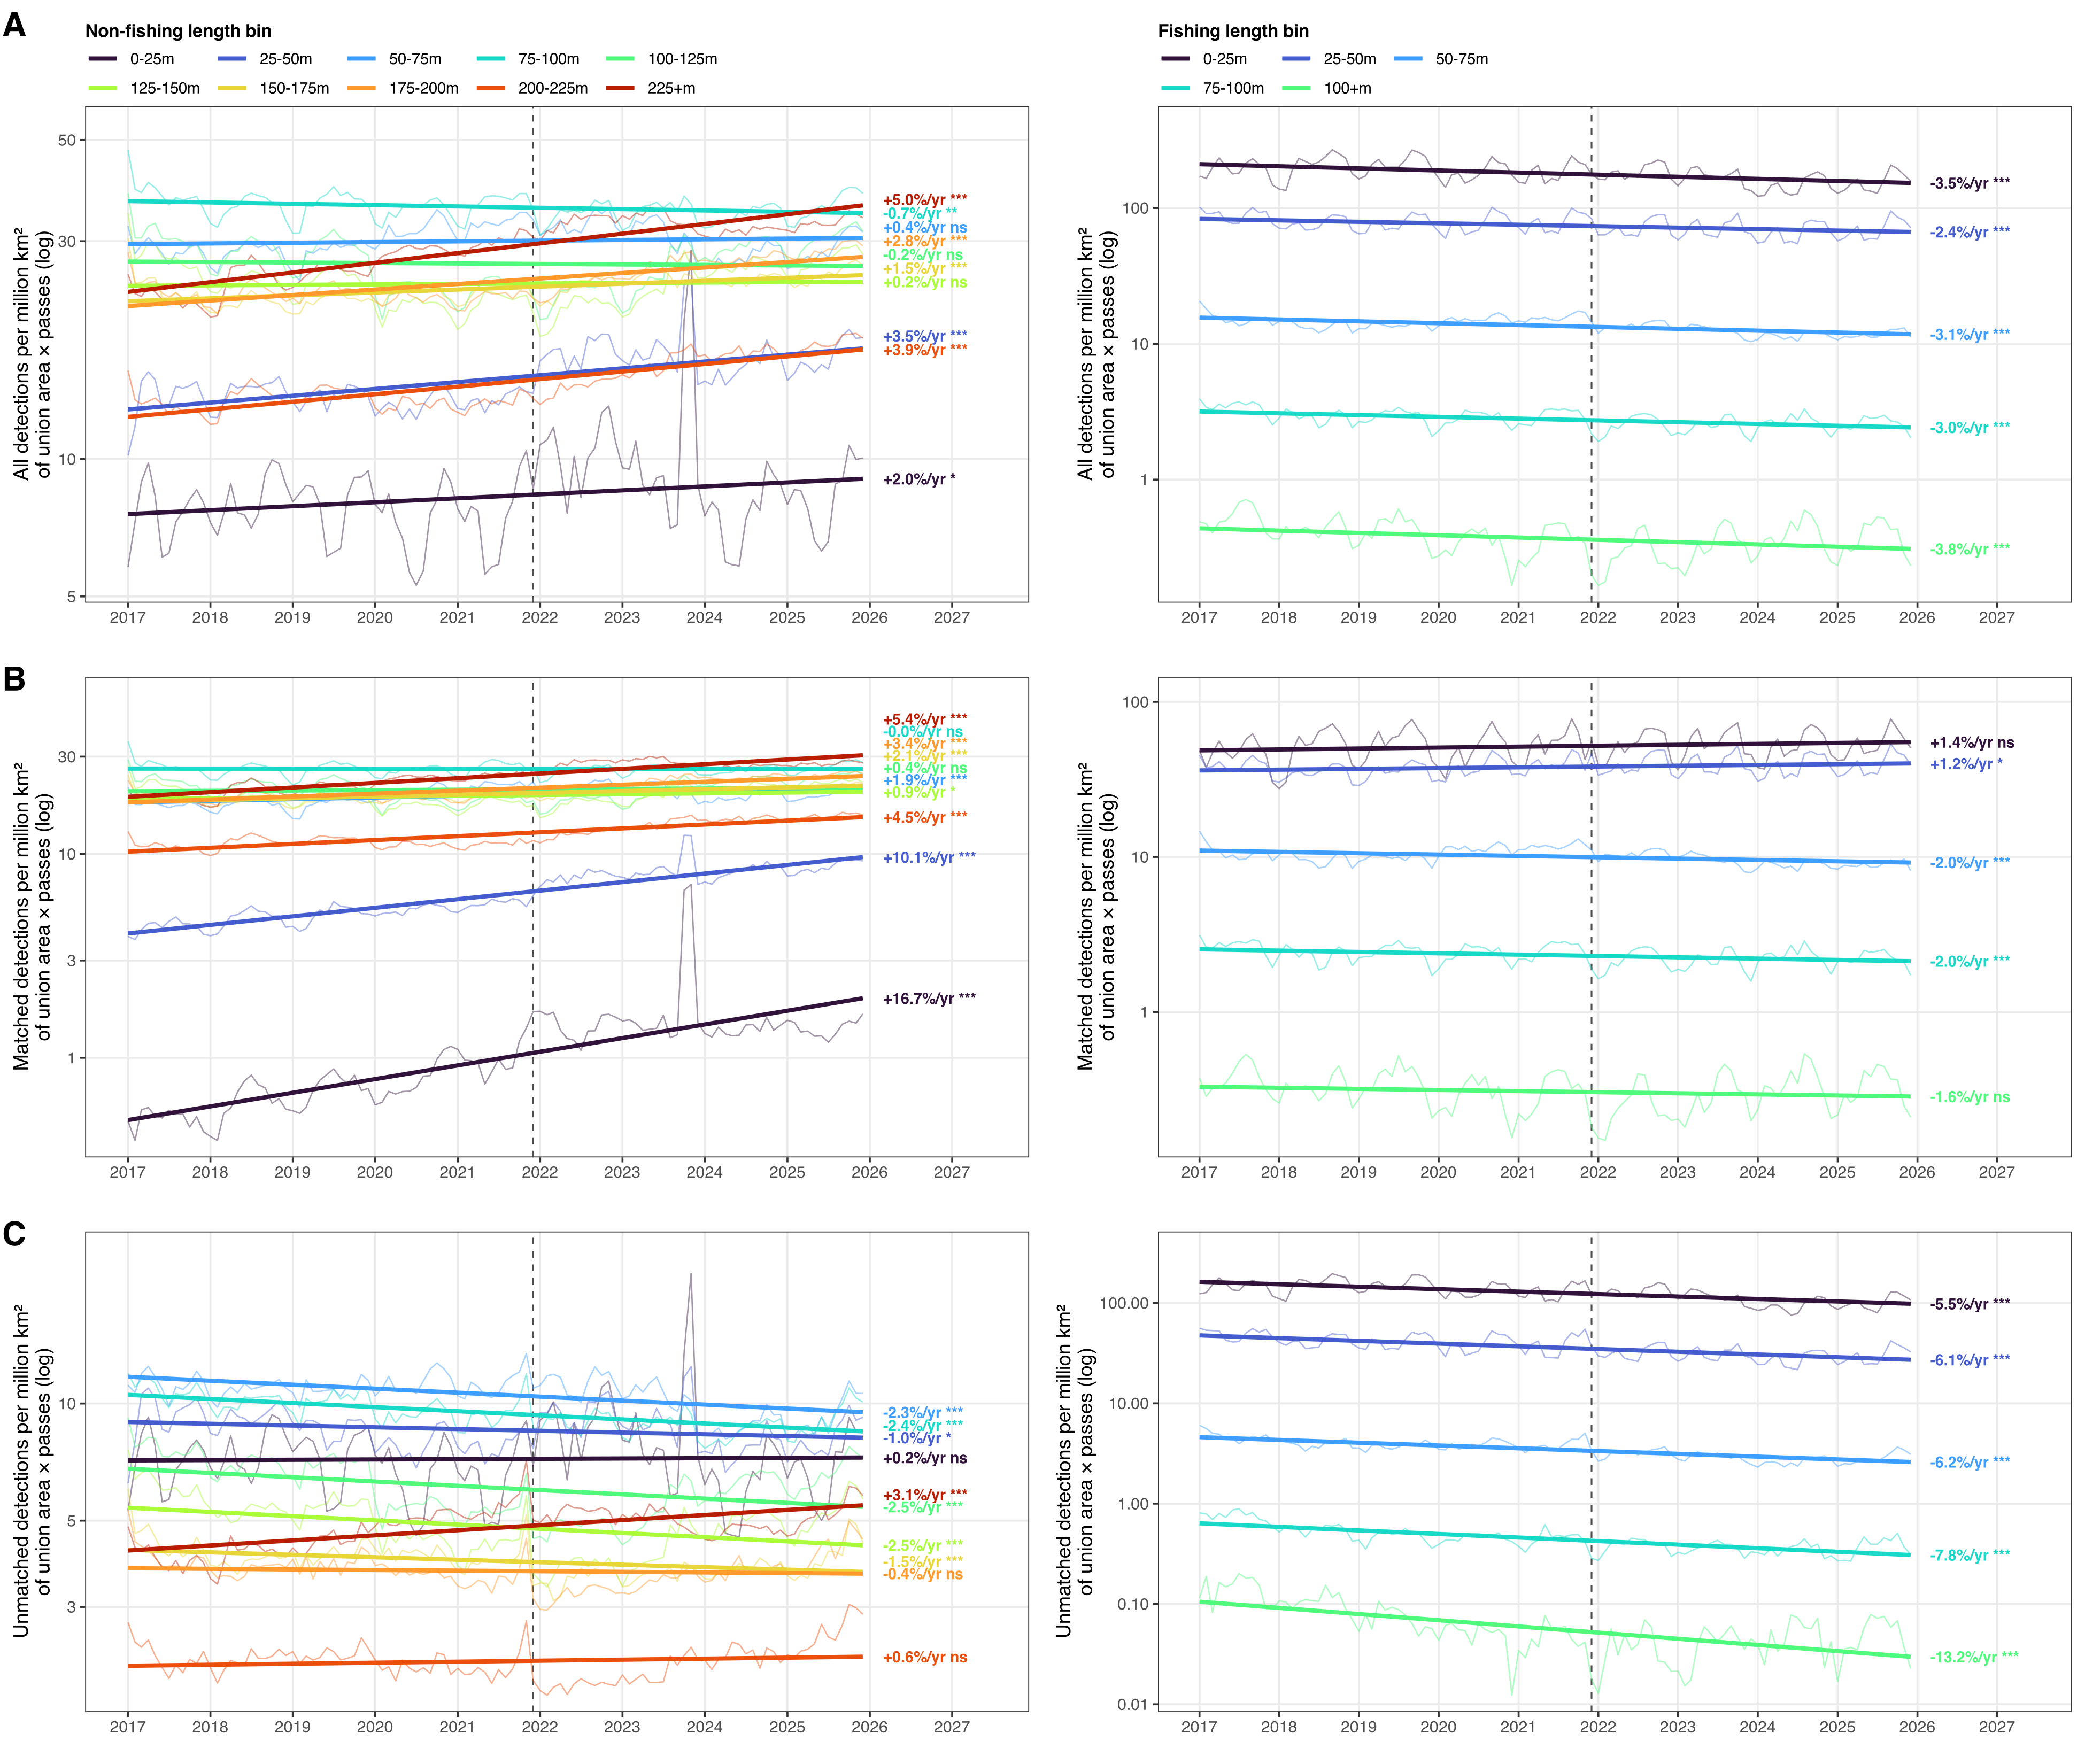
\includegraphics[width=\columnwidth]{figures/figS-density-by-match-status-1.png}
    \caption{S1 detection density by length bin, split into total, AIS-matched and unmatched detections, for fishing and non-fishing fleets, 2017--2025. Density is expressed per unit of S1 sampling effort on the same measure our emissions models use to normalize their detection features (detections per 10\textsuperscript{6} km² of per-scene imaged area summed across scenes), so the three series share a denominator and are additive. Axes are log scaled. Thin lines are monthly values; thick lines are ordinary least squares fits of log density on time over the full period, labeled with the fitted trend in percent change per year and its significance from the slope's two-sided $t$ test (*** $p<0.001$, ** $p<0.01$, * $p<0.05$, ns otherwise).}
    \label{fig:figS-density-by-match-status}
\end{figure}

Reallocation between our components, however, holds only where S1 had already detected the vessel. Vessels too small or too close to shore to be reliably detected, or operating outside the imaged footprint, which accounts for a fifth of our AIS-based emissions, contribute nothing to the S1-unmatched component and enter the fused total for the first time when they begin broadcasting. Because AIS carriage and reception expanded over the study period, that unobserved fraction was larger at the start of the series than at the end, so part of the measured growth in the fused total is that gap closing rather than activity rising. Supplementary Fig. \ref{fig:figS-density-by-match-status} (panels b and c) shows this happening: among non-fishing vessels under 25 m, matched detections per unit of observing effort rise at 16\% per year while unmatched detections stay flat, so the growth there is added to the fused total rather than transferred within it. A 150\% increase in passenger vessels under 25 m over eight years in our AIS record (Supplementary Fig. \ref{fig:figS-passenger-size-panels}) is difficult to reconcile with new construction; most of these vessels were more likely already at sea, unobserved by S1, and became visible as AIS carriage and reception expanded. That our fused trend closely tracks the AIS-only trend, only slightly shallower at 35\% against 44\% growth between 2017 and 2025, is consistent with this: some genuine reallocation occurs, but much of the measured growth enters directly through AIS.

Our fused trend is therefore better read as an upper estimate of the underlying growth than as a measurement of it. This does not make the near-flat trends of the other inventories correct. The reconciliation comes from the part of the fleet our approach captures without ambiguity: non-fishing vessels of 150 m and above, where AIS carriage was already saturated at the start of our series (Supplementary Fig. \ref{fig:figS-ais-carriage-saturation-by-size}). AIS-based emissions from this segment rose 29\% between 2017 and 2025 (Supplementary Fig. \ref{fig:figS-inventory-comparison-all-sources}, panel d). S1-unmatched emissions are not disaggregated by vessel size, so we cannot give a fused figure for this segment separately. The growth that remains once observational expansion is set aside is thus lower than our headline figure, but nowhere near the stability the other inventories describe: even confined to this segment, AIS-based emissions grew at a compound annual rate of 3.20\%, nearly twice that of the fastest-growing bottom-up inventories, more than three times that of global emissions across all sectors, and about six to seven times that of all other transportation modes combined (Supplementary Fig. \ref{fig:figS-inventory-comparison-all-sources}, Supplementary Table \ref{tab:inventory_growth_comparison}).


\end{document}
